%%
%% Copyright (C) 2010 by Andreas Dräger
%% ... (license header) ...
%%
\documentclass[ % MUST BE THE VERY FIRST COMMAND
  a4paper,                % Paper size
  12pt,                   % Base font size
  headsepline,            % Line under header
  numbers=noenddot,       % Chapter/section numbers without trailing dot
  captions=oneline,       % One-line captions if they fit
  captions=tableheading,  % Table captions above table (KOMA style)
  BCOR=12mm,              % Binding correction
  headinclude,            % Header part of type area calculation
  chapterprefix,          % Use "Chapter X" prefix
  appendixprefix,         % Use "Appendix X" prefix
  index=totoc,            % Add index to table of contents
  bibliography=totoc      % Add bibliography to table of contents
]{scrbook}

% --- Essential Setup ---
\usepackage[utf8]{inputenc} % Input encoding. CRITICAL.
\usepackage[T1]{fontenc}    % Output font encoding. CRITICAL.
\usepackage[ngerman, english]{babel} % Language support. CRITICAL, load ONCE here.


\usepackage{amsmath} % <--- Needed for \textsubscript
\usepackage{booktabs}
\usepackage{multirow}
\usepackage{rotating}
\usepackage{graphicx}
\usepackage{subcaption}
\usepackage{caption}
\usepackage{tocbasic} % Added to resolve \sf@counterlist issue
\usepackage{geometry} % Optional, for margins
\usepackage{hyperref} % For \href if used elsewhere, though not in table notes now
\usepackage{scrhack}
\usepackage{natbib}

% --- Custom Dissertation Style ---
% Loads most packages as defined in dissertation.sty
\usepackage{dissertation}

% --- Packages NOT loaded by dissertation.sty ---
\usepackage{siunitx}        % REQUIRED. Load explicitly.
\usepackage{svg}            % REQUIRED. Load explicitly.
\usepackage{ragged2e}       % REQUIRED. Load explicitly.
\usepackage{enumitem}       % REQUIRED. Load explicitly.
\usepackage{threeparttable} % REQUIRED. Load explicitly for tables with notes (\tnote).
\usepackage{makecell}       % REQUIRED. Load explicitly for multi-line cells.

\usepackage{cleveref} % For smarter referencing like \cref{}
\usepackage[version=4]{mhchem}
\usepackage{float}

% --- SIunitx Configuration ---
\DeclareSIUnit{\year}{yr}
\DeclareSIUnit{\hour}{h}
\DeclareSIUnit{\liter}{L}
\sisetup{
  separate-uncertainty = true,
  table-align-uncertainty = true,
  table-align-exponent = false,
}

% --- Robustify Commands ---
% \robustify{\pm} % <<<--- COMMENTED OUT FOR NOW to avoid 'not a macro' error.

% --- Hyperref Setup ---
% Apply detailed settings AFTER hyperref has been loaded by dissertation.sty
\hypersetup{ % <<<--- THIS BLOCK BELONGS HERE
    bookmarksopen={true},
    bookmarksopenlevel={0},
    bookmarksnumbered={true},
    breaklinks={true},
    colorlinks={false},
    pdfborder={0 0 0},
    linkcolor={blue},
    citecolor={blue},
    urlcolor={blue},
    pdfpagemode={UseOutlines},
    pdftitle={\thethesis},
    pdfauthor={\thename},
    pdfsubject={Dissertation},
    pdfkeywords={\thekeywordlist},
    pdfview={FitV},
    pdffitwindow={true},
    pdfstartview={FitV},
    pdfnewwindow={false},
    pdfdisplaydoctitle={true},
    plainpages={false},
    unicode={true}
}

% --- KOMA-Script Compatibility ---
% Load scrhack late. MUST be loaded explicitly.
\usepackage{scrhack}

% --- Metadata Setup ---
% CALL the commands defined in dissertation.sty to set document specifics.
% <<<--- THIS BLOCK BELONGS HERE
\degree{M.Sc.}
\name{Nicolás Riveras Muñoz}
\thesis{Biological soil crust and climate effects on soil stabilization, erosion, and nutrient dynamics across the Chilean Coastal Range}
\keywordlist{list, of, comma, separated, keywords}
\hometown{Puente Alto}
\dean{Prof.~Dr.~Thilo Stehle}
\reviewerone{Prof.~Dr.~Thomas Scholten}
\reviewertwo{Dr.~Peter Kühn}

% \doublespacing

% --- Hyphenation ---
\selectlanguage{english}
\hyphenation{
con-cen-tra-ti-ons
Bio-crusts
bio-crusts
}

% --- Title Page Setup ---
\title{\thethesis}
\author{\Large Dissertation\\ % Content for the author field
\normalsize der Mathematisch-Naturwissenschaftlichen Fakult\"at\\
\normalsize der Eberhard Karls Universit\"at T\"ubingen\\
\normalsize zur Erlangung des Grades eines\\
\normalsize Doktors der Naturwissenschaften\\
\normalsize (Dr.~rer.~nat.)}
\date{\ \\[2ex]\normalsize vorgelegt von\\ % Content for the date field
\thedegree~\thename\\
\normalsize aus \thehometown}
\publishers{\normalsize T\"ubingen\\\normalsize 2025} % Content for the publishers field
\lowertitleback{ % Content for the back of the title page
    Gedruckt mit Genehmigung der Mathematisch-Naturwissenschaftlichen Fakult\"at der
    Eberhard Karls Universit\"at T\"ubingen. \\ \\ \\
    \begin{tabular}{@{}lp{.8\textwidth}@{}}
    Tag der m\"undlichen Qualifikation:& XX.XX.2025\\
    Dekan:                             & \thedean\\
    1.~Berichterstatter:               & \thereviewerone\\
    2.~Berichterstatter:               & \thereviewertwo\\
\end{tabular}}

% --- Selective Compilation ---
% \includeonly{tex/Introduction, tex/Methodology}

% ==============================================================================
\begin{document} % <<<--- MARKS THE START OF THE ACTUAL DOCUMENT CONTENT
% ==============================================================================

\frontmatter
% \selectlanguage{ngerman} % Usually not needed here unless \maketitle uses language-specific terms
\maketitle
\selectlanguage{english} % Ensure English is active for main content

% --- Front Matter Sections ---
\chapter*{Abstract}
\markboth{Abstract}{Abstract}

Biological soil crusts (biocrusts) and climate effects profoundly shape soil stabilization, erosion, and nutrient dynamics, especially across diverse environmental gradients like the Chilean Coastal Range (arid to humid). This research explored these intricate interactions by integrating field observations, rainfall simulations, laboratory experiments, and advanced analytical techniques. The focus was on the interplay between biocrusts, microbial communities, plant roots, and fundamental soil properties.

Key findings reveal that biocrusts significantly enhance soil aggregate stability, particularly in drier regions, thereby reducing surface runoff and erosion. Their stabilizing influence, however, lessens in humid climates where dense vegetation becomes the dominant factor. Biocrusts modify hydrological pathways, typically decreasing surface flow while sometimes increasing percolation. They also modulate carbon (C) and nitrogen (N) fluxes in climate-dependent ways, influencing both sediment-bound and dissolved nutrient transport.

The critical role of microbial communities in soil aggregation and development was confirmed, with their activity and resilience strongly linked to climate legacy and moisture patterns (e.g., wetting-drying cycles). Plant roots emerged as powerful drivers of macroaggregation, exerting distinct influences during their living (rhizosphere) and decaying (detritusphere) phases, which in turn affects microbial succession and organic matter protection. Overall, this work highlights the interconnected, context-dependent nature of these biotic and abiotic factors in governing soil structure and function.


\selectlanguage{ngerman}
\chapter*{Kurzfassung}
\markboth{Kurzfassung}{Kurzfassung}

\begin{justify}
Biologische Bodenkrusten (Biokrusten) und Klimaeffekte prägen maßgeblich die Bodenstabilisierung, Erosion und Nährstoffdynamik, insbesondere entlang diverser Umweltgradienten wie der chilenischen Küstenkordillere (arid bis humid). Diese Forschung untersuchte diese komplexen Wechselwirkungen durch die Integration von Feldbeobachtungen, Regensimulationen, Laborexperimenten und fortschrittlichen Analysetechniken. Der Fokus lag auf dem Zusammenspiel zwischen Biokrusten, mikrobiellen Gemeinschaften, Pflanzenwurzeln und grundlegenden Bodeneigenschaften.

Wichtige Ergebnisse zeigen, dass Biokrusten die Aggregatstabilität des Bodens signifikant erhöhen, besonders in trockeneren Regionen, wodurch Oberflächenabfluss und Erosion reduziert werden. Ihr stabilisierender Einfluss nimmt jedoch in humiden Klimazonen ab, wo dichte Vegetation zum dominierenden Faktor wird. Biokrusten modifizieren hydrologische Pfade, indem sie typischerweise den Oberflächenabfluss verringern, während sie manchmal die Perkolation erhöhen. Sie modulieren auch Kohlenstoff- (C) und Stickstoff- (N) Flüsse auf klimaabhängige Weise und beeinflussen sowohl den sedimentgebundenen als auch den gelösten Nährstofftransport.

Die entscheidende Rolle mikrobieller Gemeinschaften bei der Bodenaggregation und -entwicklung wurde bestätigt, wobei ihre Aktivität und Resilienz stark mit Klima-Legacy-Effekten und Feuchtemustern (z.B. Benetzungs-Trocknungs-Zyklen) verknüpft sind. Pflanzenwurzeln erwiesen sich als starke Treiber der Makroaggregation, die während ihrer lebenden (Rhizosphäre) und zerfallenden (Detritussphäre) Phasen unterschiedliche Einflüsse ausüben, was wiederum die mikrobielle Sukzession und den Schutz organischer Substanz beeinflusst. Insgesamt hebt diese Arbeit die vernetzte, kontextabhängige Natur dieser biotischen und abiotischen Faktoren bei der Steuerung von Bodenstruktur und -funktion hervor.
\end{justify}
\selectlanguage{english}
\include{tex/Acknowledgments}

% --- Tables of Contents, Figures, Tables ---
\tableofcontents
\listoftables
\listoffigures

\mainmatter
\chapter{Introduction}
\section{Biological soil crusts and soil aggregate stability along a climatic gradient}
\label{sec:BiocrustAndStabilityInCLimate}

Life has deeply shaped the surface of Earth over billions of years, actively modifying its environment within the Critical Zone--Earth's living skin--which forms the dynamic interface between the lithosphere, atmosphere, hydrosphere, and biosphere \citep{Amundson2007,Brantley2017,Dietrich2006}. The soil, a central component of this zone, mediates essential biogeochemical processes and supports terrestrial ecosystems. Although soil is subject to constant reshaping by erosion, weathering, and tectonic activity \citep{Scholten2017}, organisms, particularly biological soil crusts (biocrusts), significantly influence its structural integrity and stabilization.

Biocrusts are formed from complex interactions among diverse organisms, including photoautotrophs such as cyanobacteria, algae, lichens, and bryophytes, and heterotrophs such as bacteria, fungi, and archaea, which intertwine with soil particles through their own filamentous structures and polysaccharide-based adhesives \citep{Belnap2016,Gao2017,Weber2022,Xiao2022}. This intricate biological network establishes a cohesive, mesh-like layer that firmly binds the uppermost soil surface, functioning as a protective, living skin on Earth's surface. Biocrust enhance soil aggregate stability by physically protecting soil aggregates, sheltering organic matter, and facilitating microbial colonization.

The stabilizing role of biocrusts is especially crucial in arid environments, where their drought tolerance and low water requirements make them the predominant biological cover \citep{Chen2020,Oliver2005}. This resilience comes from their ability to remain dormant during extended dry periods, reviving rapidly upon rewetting, even after complete desiccation, a capability attributed to the lack of specialized desiccation control structures like stomata or impermeable cuticles \citep{Maegdefrau1951,Proctor2007,Thielen2021}. Consequently, biocrust water content directly reflects the humidity of the surrounding environment, making them uniquely adapted to arid and semi-arid regions \citep{Colesie2016, Grote2010}. Under these conditions, biocrust-induced soil stability achieves its maximum impact, significantly reducing erosion susceptibility and facilitating soil formation processes.

However, as climate humidity increases along a gradient towards more temperate conditions, vegetation competes more effectively and biocrusts are often relegated to resource-limited niches \citep{Budel2016}. In temperate regions, biocrusts stablishes on bare soils or soils with minimal plant development, where conditions such as high salinity, low nutrient availability, and limited water availability mirror the limiting conditions of arid landscapes \citep{Corbin2020}. Thus, the interplay between biocrusts, microbial communities, and plant roots shifts along this climatic gradient, diminishing, but not eliminating, the protagonism of biocrusts on soil stability, structure and size distribution of soil aggregates.

\section{Microbial communities as drivers of aggregate structure}
\label{sec:MicrobialCommunitiesAggregateStructure}

Soil, far from being an inert substrate, is a dynamic and living entity teeming with a vast, often underappreciated, majority: microbial communities. These microscopic organisms, including bacteria, archaea, fungi, and protists, are the main drivers of soil development and functioning, influencing almost every aspect of terrestrial ecosystems \citep{Bardgett2014}. Their ubiquity and sheer abundance, with cell counts often reaching billions per gram of soil, underscore their significance in biogeochemical processes \citep{Nunan2001}. Microorganisms mediate complex nutrient cycles that involve carbon, nitrogen, and phosphorus, transforming organic matter and making essential elements accessible for plant uptake \citep{Schimel2012}. Furthermore, they actively participate in the weathering of minerals, contributing to soil development and releasing nutrients into the environment \citep{Barkay2001,Burford2003}. Their metabolic activities influence soil pH, redox conditions, and the overall chemical environment, thus creating diverse microhabitats that sustain a wide variety of life forms \citep{Brehm2005}.

The resilience and adaptability of microbial communities is perhaps most strikingly demonstrated in extreme environments. Arid climates, characterized by drastic temperature fluctuations, minimal precipitation, and limited nutrient availability, provide compelling examples of how microbial life thrives under harsh conditions. Research in these arid ecosystems has revealed unexpectedly high abundances of diverse microorganisms, even in extremely dry desert environments \citep{Bernhard2018,Newsham2016}. This ability to withstand environmental stress makes desert soils particularly valuable for understanding the potential effects of climate change on microbial communities \citep{Pearce2012}. Studying these environments offers valuable insights into the limits of life and the adaptive strategies microorganisms employ when confronted with adversity. Such knowledge is invaluable for understanding the potential responses of microbial communities to ongoing and future environmental changes.

The connection between microbes and the development of soil structure is profound. Microorganisms colonize raw mineral substrates such as saprolite or newly formed desert soils, initiating a complex successional process that transforms bare rock into fertile soil \citep{Lazaro2008,Stradling2002}. They contribute to mineral weathering through the production of organic acids and other metabolites that dissolve rock surfaces \citep{Bajerski2013,Mavris2010,Styriakova2012}. Along the Chilean Coastal Range, climate distinctly shapes microbial community composition, driving shifts in microbial functions, including their capability to stabilize soil aggregates \citep{Bernhard2018}. Microbes decompose organic matter derived from plant and animal residues, releasing nutrients and contributing to the formation of soil organic matter, a critical component of soil structure and fertility \citep{Oades1993}. Furthermore, microbial communities actively participate in the formation of soil aggregates by exuding substances like polysaccharides, which act as a glue, binding soil particles together and creating a stable soil structure \citep{Martens1992,SchlechtPietsch1994}. Consequently, climatic-driven microbial succession directly influences soil aggregation, which is essential for maintaining soil stability, enhancing water infiltration, reducing soil erodibility, and ultimately fostering ecosystem development.

\section{Climate as a driver of soil and microbial dynamics}
\label{sec:ClimateMicrobialDynamics}

Climate stands as a primary architect of soil, profoundly influencing its formation, structure, and function \citep{Jenny1941}. Temperature and precipitation regimes, along with evapotranspiration rates, dictate the weathering of parent material, the accumulation and decomposition of organic matter, and the development of distinct soil horizons \citep{Scholten2017}. These climatic factors also exert a strong influence on the soil water balance, which in turn affects nutrient availability and the overall biogeochemical cycling within the soil ecosystem \citep{Eldridge2020,Thielen2021}.

The influence of climate extends beyond the purely abiotic realm, shaping the composition and activity of microbial communities that inhabit the soil \citep{Nemergut2005}. Different climatic conditions select for distinct microbial populations, influencing their functional capabilities and the biogeochemical processes they mediate \citep{Newsham2016}. For instance, arid environments, characterized by low precipitation and high temperatures, harbor specialized microbial communities adapted to these extreme conditions \citep{Pearce2012}. These microbial communities play a vital role in initial soil formation and nutrient cycling, even in the face of resource scarcity \citep{Bernhard2018}. Our own studies in the Chilean Coastal Range revealed distinct patterns in soil properties and microbial communities along a climate gradient \citep{Bernhard2018}. Interestingly, these trends often followed specific, rather than homogeneous, patterns, indicating the presence of threshold processes and buffering mechanisms in soil ecosystems \citep{Bernhard2018}.

The development and distribution of biological soil crusts (BSCs) are also intricately linked to climate. Water availability, driven by precipitation and evapotranspiration, is a major determinant of biocrust cover and composition \citep{Bowker2016}. Arid regions tend to favor biocrust dominance due to the scarcity of vascular plant cover \citep{Colesie2016,Grote2010}, while more humid climates support greater plant diversity, leading to a mosaic of biocrusts interspersed with plants \citep{Issa1999}. The protective effects of BSCs against erosion and their influence on soil hydrology also vary depending on climate, with potential trade-offs between runoff reduction and water infiltration \citep{Thielen2021}. These findings demonstrate the importance of considering climate not only as a driver of soil properties but also as a key factor shaping microbial communities and the distribution and functionality of biocrusts. The Chilean Coastal Range, with its dramatic gradient from arid to humid conditions, provides a natural laboratory for investigating these complex interactions. This gradient allows us to explore how the interplay of climate, soil, microbes, and biocrusts shapes the Earth’s surface across varying environmental conditions. Furthermore, understanding how climate influences these components individually and in combination is crucial for predicting how soil ecosystems will respond to future environmental changes. The non-linear nature of some of these climate-driven changes, coupled with the potential existence of thresholds in soil processes across environmental gradients, highlights the need for comprehensive research in diverse climatic settings \citep{Bernhard2018}.

\section{Influence of plant roots and interactions with biocrusts along the climate gradient}
\label{sec:PlantRootsBiocrust}

Soil, far from being a simple mixture of minerals and organic matter, is a dynamic and intricate web of interactions between diverse biotic and abiotic components. Central to this web are plant roots, which exert a profound influence on the surrounding soil environment, driving structural changes, altering nutrient availability, and shaping microbial communities \citep{Hinsinger2009}. These complex interactions among roots, microbes, and soil particles constitute a fundamental axis supporting soil development and ecosystem functioning.

Roots physically restructure the soil matrix through growth and penetration, creating channels and pores, thereby enhancing aeration and water infiltration \citep{Bruand1996}. This process of bioturbation is particularly relevant in developed soils, where root systems establish intricate networks of interactions with the surrounding environment. Moreover, roots release a variety of compounds, known as rhizodeposits, including sugars, amino acids, and organic acids, which serve as primary substrates for soil microorganisms \citep{Hinsinger2009,Rasse2005}. This concentrated release of labile carbon in the rhizosphere fuels microbial activity, creating a "hotspot" of biological processes \citep{Hinsinger2009}.

The impact of roots, however, extends beyond the immediate vicinity of the living root. As roots senesce and decompose, they enter the detritusphere, a zone characterized by the breakdown of plant-derived organic matter \citep{Vidal2018}. In this zone, the legacy of roots persists as decomposed root material contributes to soil organic matter formation and influences the structure and stability of soil aggregates \citep{Six2004}. The transition from rhizosphere to detritusphere marks a shift in the microbial community, as the readily available carbon from rhizodeposits is replaced by more complex organic compounds derived from decaying root tissues \citep{Vidal2018}. This shift in resource availability triggers microbial succession, favoring microorganisms capable of degrading these more recalcitrant substances.

Importantly, the interactions between biocrusts and vascular plants form a dynamic feedback loop in soil ecosystems. Biocrusts, as early colonizers of bare ground, contribute to the initial stabilization of the soil surface, creating microhabitats that facilitate subsequent plant establishment \citep{BelnapBudel2016,Bowker2006}. As plants colonize and their root systems develop, they further enhance soil structure formation, promoting the accumulation of organic matter, and creating conditions for diverse microbial communities to thrive \citep{Schweizer2018,Six2004}. This positive feedback loop between biocrusts and plants drives the development from initial, unstable soil environments towards more mature and resilient soil ecosystems. Thus, along environmental gradients, plant roots progressively become primary agents of aggregate stability, influenced indirectly but significantly by earlier biocrust colonization and microbial activity.

\section{Biocrusts, hydrological processes, and nutrient fluxes influencing soil erosion}
\label{sec:BiocrustFluxes}

Climatic conditions strongly shape biocrust composition, morphological characteristics, and ecological functions, thus influencing hydrological processes, nutrient cycling, and susceptibility to soil erosion \citep{Belnap2003,ConcostrinaZubiri2014}. In arid environments, biocrusts dominated by cyanobacteria and lichens typically form smooth, compact surfaces enriched with microbial biomass and extracellular polysaccharides (EPS), profoundly affecting surface hydrology \citep{RodriguezCaballero2018,Weber2022}. Such biocrust structures frequently lead to surface pore clogging, potentially increasing runoff initiation but simultaneously reducing sediment loss by enhancing aggregate stability and protecting soil organic matter \citep{Kidron2021}. Conversely, in humid climates, biocrusts with higher proportions of bryophytes and fungi possess rougher surfaces that promote water retention, facilitate infiltration, and reduce runoff, thereby strongly influencing sediment transport and nutrient dynamics \citep{RiverasMunoz2022,Seitz2017}.

These functional differences across climate conditions emphasize the critical role biocrusts play in regulating carbon (C) and nitrogen (N) fluxes, erosion dynamics, and soil fertility. Biocrusts act as initial stabilizers of soil organic matter, even preceding plant colonization, thus shaping early nutrient cycling pathways \citep{Belnap2007,Young2022}. Furthermore, by physically absorbing raindrop energy, trapping sediment, and promoting microbial-driven aggregate formation, biocrusts provide a protective barrier against erosion, influencing water and sediment fluxes \citep{Costa2018,Xiao2022}.

However, the way in which biocrust-mediated hydrological processes, nutrient cycling, and erosion control shift across gradients of temperature and humidity remains uncertain. These functional patterns are complex and nonlinear, reflecting intricate interactions between biocrust structure, microbial activity, vegetation competition, and climatic variability rather than a simple linear climatic transition \citep{Bernhard2018,RiverasMunoz2025}.

\section{Understanding biocrusts across a climatic gradient}
\label{sec:BiocrustClimate}

Soil represents an intricate web of interactions among diverse organisms, where biocrusts play a pivotal climate-dependent role in stabilizing aggregates, regulating erosion, and controlling water and nutrient fluxes. This biocrust-mediated stabilization effect is most pronounced in arid regions due to minimal vegetation, decreasing in relative importance but persisting as climates become more humid. Along the Chilean Coastal Range, this dynamic illustrates how biocrusts, microbial communities, and plant roots co-evolve, shaping soil structure, erosion resistance, and nutrient cycling.

Addressing these complex interactions and feedbacks is crucial for predicting how soils and associated ecosystems will respond to ongoing climate changes, especially considering the non-linear and threshold-driven nature of soil processes across environmental gradients \citep{Bernhard2018,Wang2014}. Future research should deepen understanding of these interactions, exploring quantitative relationships to inform conservation strategies and enhance ecosystem resilience in a rapidly changing world.

Understanding how biocrust functions shift across climatic gradients is critical for predicting soil ecosystem responses to environmental changes. The interactions among biocrusts, microbial communities, and plant roots along these gradients exemplify the inherent complexity and nonlinearity of soil processes \citep{Wang2014}. Biocrusts exert differing influences on soil aggregate stability, soil erodibility, water and nutrient flows, reflecting adaptive responses to variations in moisture availability, temperature, and vegetation cover \citep{Belnap2003,Weber2022}. In arid climates, biocrusts typically dominate soil surfaces, forming protective layers that significantly modulate hydrological processes, sediment transport, and microbial activity, thereby strongly influencing soil structure and organic matter dynamics \citep{Kidron2021,RodriguezCaballero2018}. However, as climatic humidity increases, the interplay between biocrusts and plant roots becomes more intricate, with intensified competition from vegetation altering microbial community composition and reshaping nutrient pathways \citep{RiverasMunoz2022,Seitz2017}. Rather than transitioning gradually, these interactions likely exhibit thresholds and complex feedback loops \citep{Wang2014}, implying that even subtle climatic shifts can substantially modify ecosystem functions \citep{Bernhard2018}. Recognizing these nonlinear responses is critical for predicting how soils—and the ecosystems they sustain—will adapt to current and future climatic changes. Addressing these knowledge gaps through quantitative assessments of biocrust-driven processes is therefore essential for developing effective conservation strategies, promoting soil health, and enhancing ecosystem resilience \citep{BelnapBudel2016,Weber2022}.

\section{Objectives and hypothesis}
\label{sec:ObjectivesHypothesis}

This research forms part of the DFG Priority Program: EarthShape: Earth Surface Shaping by Biota (DFG-SPP 1803), specifically within the subproject Microbial Engineers - Drivers of Earth Surface Development and Stabilization. The subproject aims to understand microbial processes that shape Earth's surface, focusing on the roles microorganisms play and providing a quantitative understanding of the mechanisms and microbial taxa involved under various climate conditions. It addresses these questions by: (i) experimentally investigating how microorganisms alone control the formation and transition of initial soils into resilient ecosystems; and (ii) analyzing the combined influence of microorganisms, biocrusts, and plant roots on soil surface stability and erosion under natural and controlled conditions along climatic gradients.

It is hypothesized that biocrusts enhance soil aggregate stability by physically protecting the soil surface, sheltering organic matter, altering microbial community structures, and modifying water infiltration patterns (Manuscripts 1 and 2). This stabilizing effect is expected to be most pronounced in arid climates, where biocrusts represent the primary soil cover due to minimal vegetation and limited organic matter inputs. With increasing humidity, however, the influence of biocrusts on soil stabilization is predicted to diminish, though it will not disappear entirely, due to greater water availability and competition from vegetation (Manuscript 1).

Furthermore, soil microbial communities are hypothesized to accelerate soil formation processes in arid environments when moisture and temperature conditions are favorable. Responses to simulated climate change are expected to be mediated by soil legacy effects, shaping microbial community structure and interactions over time. Bacterial diversity and adaptation processes likely reflect climatic shifts, providing insight into long-term soil developmental dynamics (Manuscript 3). Microbial communities are also expected to be crucial for soil aggregation by influencing soil structure and stability across different climates and stages of soil development. Specific microbial taxa may differentially influence aggregation processes, with their contributions being modulated by biotic and abiotic factors, including wetting-drying cycles and moisture fluctuations (Manuscript 4).

Roots are hypothesized to promote water-stable macroaggregate formation in topsoil and subsoil, with legacy effects persisting after plant death within the detritusphere (Manuscript 5). Microbial abundance near roots is expected to increase due to labile carbon availability, especially in carbon-poor subsoils. The transition from rhizosphere to detritusphere likely triggers microbial succession, favoring gram-positive bacteria as readily available carbon compounds are replaced by more complex materials. Root-derived organic matter, including rhizodeposits and litter, is presumed to significantly influence organic matter dynamics by facilitating the formation of particulate and mineral-associated organic matter, thereby shaping aggregate formation and biogeochemical processes (Manuscript 5).

Lastly, biocrusts are hypothesized to regulate hydrological processes such as runoff, sediment discharge, and percolation flows, along with associated carbon and nitrogen fluxes, thereby reducing soil erosion irrespective of climatic conditions. However, climate-specific feedbacks among these hydrological processes likely mediate carbon and nitrogen transport within biocrust-dominated ecosystems (Manuscript 2).
To test these hypotheses, the objectives of this thesis were to:
\begin{itemize}
  \item Evaluate the role of biocrusts in soil aggregate stabilization and their regulation of erosion, water, and nutrient fluxes across a climatic gradient in the Chilean Coastal Range, examining how variations in biocrust properties correlate with changes in climate and vegetation cover (Manuscripts 1 and 2).
  \item Examine how soil microbial communities influence aggregate formation and stability under different climatic and moisture regimes, as well as their responses to simulated climate-change scenarios (Manuscripts 3 and 4).
  \item Determine the influence of plant roots on soil structure development, microbial succession, and organic matter dynamics during transitions from rhizosphere to detritusphere, emphasizing their role in soil aggregate formation (Manuscript 5).
\end{itemize}
\chapter{Methodology}

\section{Study sites and experimental setting}
\label{sec:StudysitesAndExperimentalSetting}

In order to assess the climatic effect on soil and its interactions with biocrusts, five study sites distributed between latitudes from \ang{26;6}~S to \ang{37;48}~S and over \SI{1315}{\kilo\meter} were established in the Chilean Coastal Range (Figure \ref{fig:location-map}): Pan de Azúcar National Park (PdA), Santa Gracia Natural Reserve (SG), Quebrada de Talca Private Reserve (QdT), La Campana National Park (LC) and Nahuelbuta National Park (NA), corresponding to arid, coastal semi-arid, inland semi-arid, Mediterranean and humid climates, respectively \citep{Bernhard2018}.

\begin{figure}[H]
	\centering
	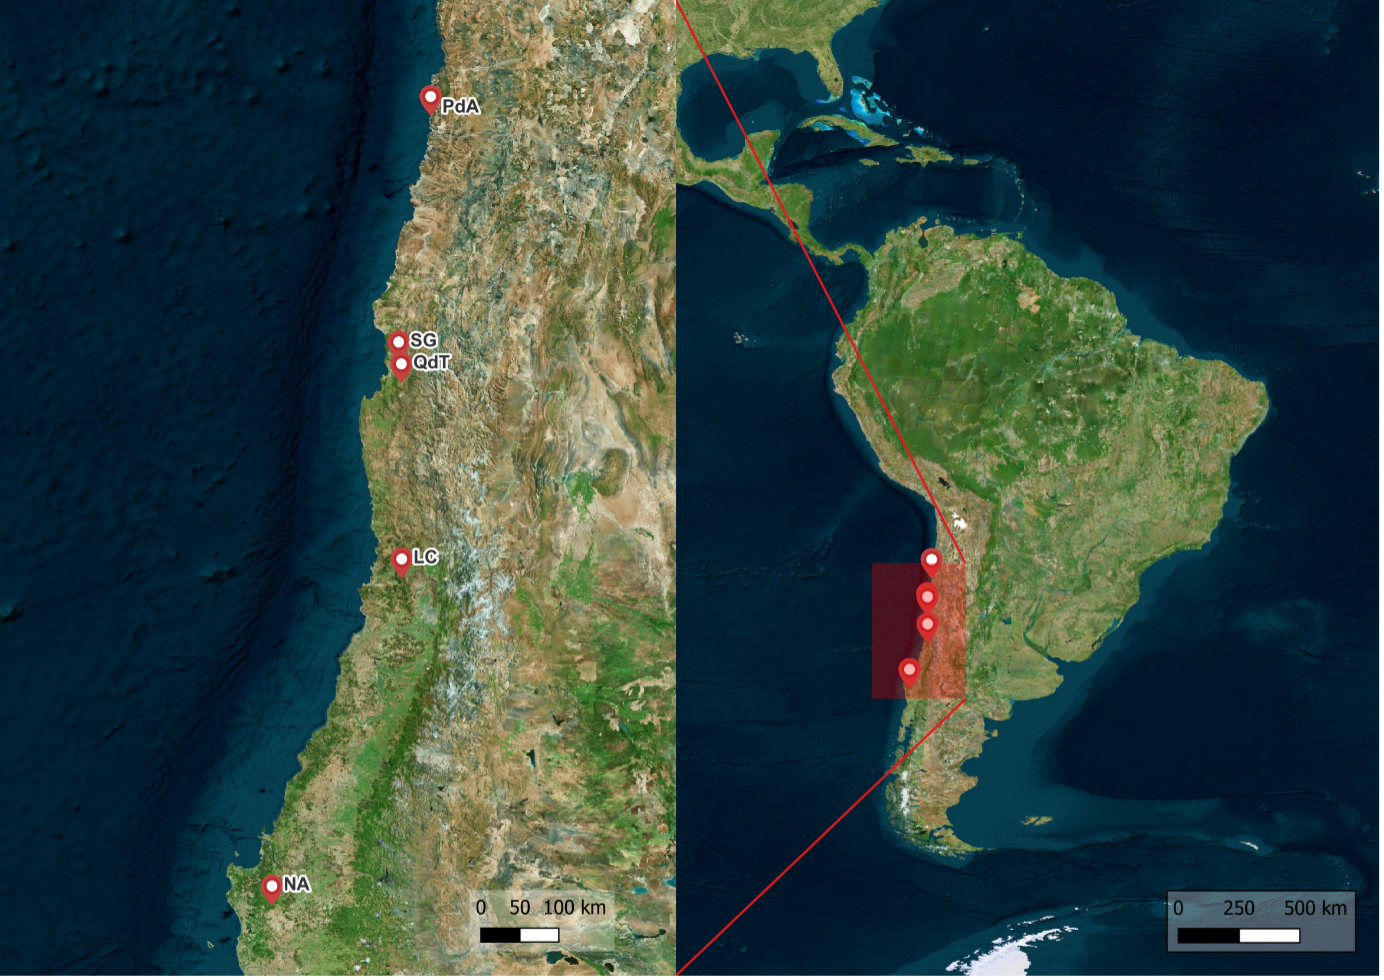
\includegraphics[width=1\textwidth]{img/location-map.png}
	\caption{Location of study sites relative to South America. From north to south: Pan de Azúcar (PdA), Santa Gracia (SG), Quebrada de Talca (QdT), La Campana (LC), and Nahuelbuta (NA).}
	\label{fig:location-map}
\end{figure}

The study sites are comparable in geology, geomorphology, land use, and influence of glaciers and volcanoes \citep{Bernhard2018}. The parent material in all the study sites is granitoid \citep{Bernhard2018}. The dominant topography is generally fluvial valleys, and the sites had no glacial influence during the last glaciation \citep{Hulton2002}. The sites are located within nature protection areas, with limited anthropogenic influence compared to the surrounding areas. Despite this, cattle occasionally enter these locations, and goats, mules, and donkeys have been reported to SG \citep{Armesto2007}.

The mean annual temperature (MAT) decreases from north to south (PdA: \SI{16.8}{\celsius}, SG: \SI{13.7}{\celsius}, QdT: \SI{14.3}{\celsius}, LC: \SI{14.1}{\celsius}, NA: \SI{6.6}{\celsius}). The mean annual precipitation (MAP) in the study sites increases from north to south (PdA: \SI{12}{\milli\metre\,\year^{-1}}, SG: \SI{66}{\milli\metre\,\year^{-1}}, QdT: \SI{109}{\milli\metre\,\year^{-1}}, LC: \SI{367}{\milli\metre\,\year^{-1}}, NA: \SI{1469}{\milli\metre\,\year^{-1}}) with similar rainfall distribution mostly concentrated in winter months (May to August) \citep{Bernhard2018,Santibnez2017}. The elevation of the sites increases from north to south (PdA: \SIrange{329}{351}{\meter}, SG: \SIrange{642}{720}{\meter}, QdT: \SIrange{565}{611}{\meter}, LC: \SIrange{708}{732}{\meter}, NA: \SIrange{1200}{1270}{\meter}). Paleoclimate modeling studies \citep{Mutz2018} indicate that these climate patterns have been persistent since the late Pliocene; thus, the study sites represent the long-term impact of climate on the soil \citep{Ewing2006}. \citet{Bernhard2018} classified soils in the study sites as Regosols in PdA, Cambisols for SG and LC, and Umbrisols in NA. In general, pedogenic properties such as soil depth, clay content, organic matter accumulation, porosity, and activity ratio are positively correlated with site humidity \citep{Bernhard2018}.

For each of the 5 study sites (Figure \ref{fig:location-panel}), 5 plots of \SI{1}{\meter}~$\times$~\SI{1}{\meter} were set up as replicates (P1 to P5). Each plot was assigned in the top-slope position with a south-facing exposition, considering a high presence of site-typical biocrust communities, similar slope and aspect, lack of anthropogenic disturbance, and a maximum distance of \SI{30}{\meter} between each plot. Within each plot, patches with the highest available biocrust cover were included as treatment BSC+, and nearby bare soil without biocrust cover was defined as control (BSC-). \newline

\begin{figure}[h!]
	\centering
	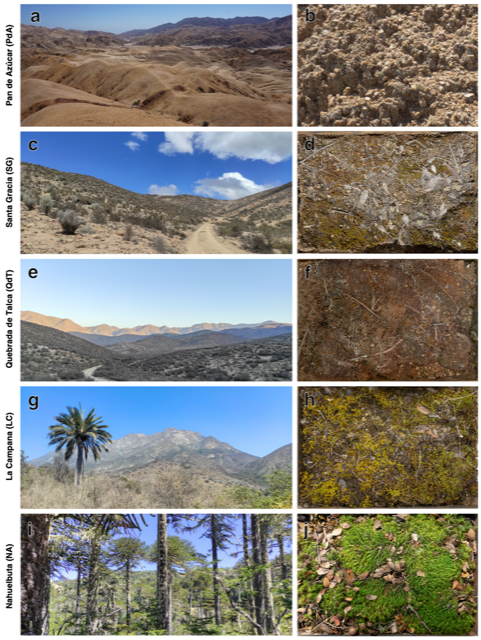
\includegraphics[width=1\textwidth]{img/location-panel.png}
	\caption{General view (a, c, d, g, and i) and sampled biocrust (b, d, f, h, and j) of PdA, SG, QdT, LC, and NA.}
	\label{fig:location-panel}
\end{figure}

\FloatBarrier

\section{Field methods}
\label{sec:FieldMethods}
\subsection{Biocrust sampling and characterization}

In a first field campaign during March 2019, biocrust patches of approximately \SI{100}{\centi\metre^{2}} were collected in PdA, SG, LC and NA and identified according to \citet{Lange2016}. The patches were collected in the field by carefully detaching the biocrust layer, removing the loose soil, and storing it in paper envelopes after air-drying for every research plot. \citet{Samolov2020} describes a biocrusts dominance in PdA with cover of up to 40\%. The other study sites are dominated by higher vegetation that limits the cover of biocrust up to 15\% in SG and 5\% in LC and NA. Sampled communities showed all typical biocrust classes from cyanobacteria, algae, fungi, lichens, liverworts, and mosses. The species composition further showed a graduating change from lichen-dominating biocrusts in the northernmost site to bryophyte-dominating biocrusts in the southernmost site. Biocrusts in NA were specifically found in zones of forest soil disturbance. Bryophyte-dominated biocrusts were sampled with rhizoids down to \SI{5}{\milli\metre} depth; all other communities were down to \SI{2}{\milli\metre}. Dominant macroscopic biocrust species were determined for each of the four sites to the genus level by morphological characteristics using a stereomicroscope (Leitz TS, Wetzlar, Germany), a transmitted-light microscope (Leitz Laborlux S, Wetzlar, Germany), and ultraviolet light. Species groups were separated into bryophytes \citep{Ardiles2014,BednarekOchyra2001,Cuvertino2012,He1998,Lightowlers2013} and lichens \citep{Galloway2007} and assigned to the different regions (Table \ref{tab:taxonomical_composition}). \citet{Bernhard2018}, based on morphological identification of enrichment cultures, reported that the biocrusts of the four studied sites were composed of 18 to 15 species of algae and cyanobacteria; where the richness of green algae increased, while the richness of cyanobacteria decreased with increasing humidity and decreasing mean annual temperature. While \citet{Samolov2020}, based on morphological and molecular traits, reported 18 species in PdA, 26 species in SG, 40 species in LC, and 27 species in NA.

\begin{table}[h!]
\centering
\caption{Taxonomical composition of mosses and lichens in the biological soil crust for the study sites along the climatic gradient.}
\resizebox{\textwidth}{!}{%
\begin{tabular}{lllc}
\hline
\textbf{Site / Division} & \textbf{Family} & \textbf{Genus} & \textbf{No. species} \\
\hline
\textbf{PdA} & & & \\
Lichens & Cladoniaceae & \textit{Cladonia} sp. & 2 \\
        & Verrucariaceae & \textit{Placidium} sp. & 2 \\
        & Lecanoraceae & \textit{Lecidella} sp. & 1 \\
        & Rhizocarpaceae & \textit{Rhizocarpon} sp. & 1 \\
\hline
\textbf{SG} & & & \\
Mosses & Pottiaceae & \textit{Syntrichia} sp. & 2 \\
       & Pottiaceae & \textit{Tortella} sp. & 2 \\
Unidentified lichens & & & 2 \\
\hline
\textbf{LC} & & & \\
Mosses & Bartramiaceae & \textit{Philonotis} sp. & 1 \\
       & Bryaceae & \textit{Bryum} sp. & 1 \\
       & Pottiaceae & \textit{Syntrichia} sp. & 2 \\
       & Pottiaceae & \textit{Tortella} sp. & 2 \\
Unidentified mosses and lichens & & & 2 + 1 \\
\hline
\textbf{NA} & & & \\
Mosses & Amblystegiaceae & \textit{Acrocladium} sp. & 1 \\
       & Amblystegiaceae & \textit{Amblystegium} sp. & 1 \\
       & Bartramiaceae & \textit{Bartramia} sp. & 1 \\
       & Bryaceae & \textit{Bryum} sp. & 1 \\
       & Dicranaceae & \textit{Campylopus} sp. & 2 \\
       & Pterigynandraceae & \textit{Myurella} sp. & 1 \\
Unidentified liverworts, lichens, fungi & & & 2 + 2 + 1 \\
\hline
\end{tabular}}
\label{tab:taxonomical_composition}
\end{table}

\FloatBarrier

\subsection{Soil sampling}

Soil sampling campaigns were primarily conducted during the austral dry season (typically January-April) to capture baseline soil conditions prior to the onset of winter precipitation. Specific sampling approaches were adapted based on the objectives of individual studies. For investigations concerning aggregate stability, moisture regime effects, and general baseline characterization across the full gradient (PdA, SG, LC, NA), bulk topsoil samples (\SIrange{0}{5}{\centi\metre} depth) were collected from each plot on mid-slope, south-facing locations using metal-core augers or by sampling from shallow soil pits (Manuscripts 1 and 4). These samples were processed in the field by sieving ($<$\SI{2}{\milli\metre}), another batch of samples was sieved and sterilized with ethanol, before being homogenized per site or kept discrete per plot depending on the experimental design and subsequently stored at \SI{4}{\celsius} pending laboratory analysis. For studies focusing on initial soil formation and rhizosphere/detritusphere dynamics (PdA, SG), distinct soil horizons (A horizon: \SIrange{0}{2}{\centi\meter}/\SIrange{0}{3}{\centi\meter}; B horizon: \SIrange{2}{3}{\centi\meter}/\SIrange{25}{40}{\centi\meter}) where sampled from excavated soil pits (Manuscripts 3 and 5). Processing involved similar steps: sieving ($<$\SI{2}{\milli\metre}), homogenization per horizon and site, and storage at \SI{4}{\celsius}.

\subsection{Rainfall simulations}

Following observations of limited soil stabilization at PdA, further rainfall simulation experiments were conducted during subsequent expeditions in 2020 and 2022 at SG, Quebrada de Talca (QdT), LC, and NA. Five \SI{1}{\meter}~$\times$~\SI{1}{\meter} plots were established as replicates at each of the four sites, consistently located on south-facing top slopes. Plot selection considered the presence of representative biocrust communities, similar slope and aspect, minimal anthropogenic disturbance, and a maximum inter-plot distance of \SI{30}{\meter}. Within each plot, runoff plots (ROPs) were established in areas with maximum biocrust cover for biocrust-present (BSC+) treatments, and adjacent biocrust-free (BSC-) locations served as controls. The experimental design was a factorial completely randomized design, incorporating four sites (SG, QdT, LC, and NA) (Figure \ref{fig:location-panel}), two biocrust conditions (BSC+ and BSC-), five replicate plots (P1-P5), and three technical replicate ROPs (R1-R3) per plot. This resulted in a total of eight treatments (site × biocrust) with 15 samples per treatment (plot $\times$ technical replicate), yielding a total sample size of n = 60.

Undisturbed soil samples for rainfall simulation were collected (Figures \ref{fig:sampling-panel}b and \ref{fig:sampling-panel}c), using piercing frames (\SI{20}{\meter}~$\times$~\SI{30}{\meter}~$\times$~\SI{7}{\meter}) (Figure \ref{fig:sampling-panel}a) and carefully installed into infiltration boxes to minimize surface and subsurface disturbance (Figure \ref{fig:sampling-panel}d). These steel boxes, designed with a triangular surface runoff gutter and a bottom outlet, captured both runoff and percolated water. Soil water content was measured using a TDR probe (Delta-T Devices Ltd. Cambridge, UK), averaging three measurements adjacent to each ROP. Biocrust cover in BSC+ ROPs was assessed using perpendicular photographs taken with a digital camera (Sony ILCE-6000, SELP1650 lens; Tokyo, Japan). Photographs were analyzed using the grid-quadrat method with a 100-subdivision grid, and biocrusts were identified visually \citep{Belnap2001}.

\begin{figure}[h!]
	\centering
	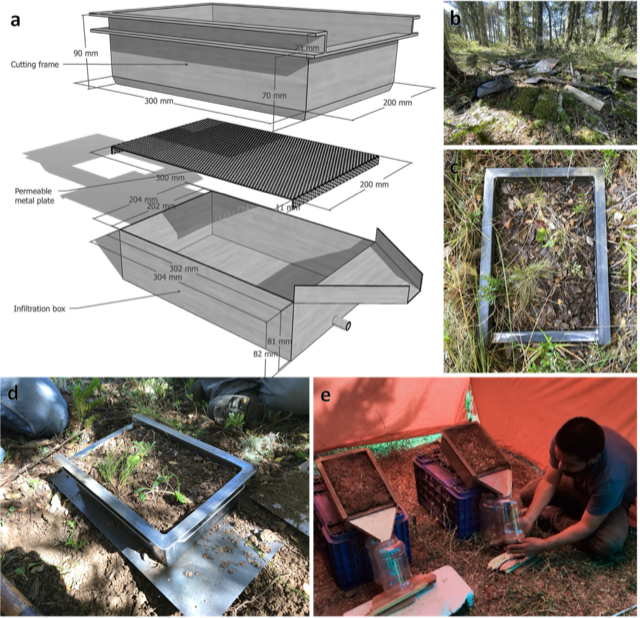
\includegraphics[width=1\textwidth]{img/sampling-panel.png}
	\caption{Construction diagram of the soil erosion flux box used in the experiment (a), general view of a plot with the presence of biocrust prior to sampling (b). (c, d) shows an installed cutting frame and the cleared and prepared soil. (e) demonstrates the setting for rainfall simulations at the Nahuelbuta (NA) study site.}
	\label{fig:sampling-panel}
\end{figure}

\FloatBarrier

Rainfall simulations were conducted near the sampling locations using the T\"ubingen rainfall simulator \citep{Iserloh2013,Seitz2015} equipped with a Lechler 460.788.30 nozzle and set to a falling height of \SI{3.5}{\meter}. Infiltration boxes were placed inside the simulator on a \ang{10} slope (Figure \ref{fig:sampling-panel}e). A rainfall event was simulated using an intensity of \SI{45}{\milli\metre\,\hour^{-1}} sustained over a 30‐minute period. According to regional intensity-duration-frequency analyses for central Chile \citep{PizarroTapia2020}, such an intensity falls within the extreme rainfall category, well above the heavy precipitation threshold even for relatively wet climates. This extreme intensity was selected to exceed the soil infiltration capacities and reliably generate surface runoff at all study sites. The time to initial runoff and percolation was recorded. Runoff and sediment-laden water samples were collected separately. Runoff volume was measured using a graduated beaker. Samples were allowed to settle by gravity for 12 hours, after which a water sample was extracted from the supernatant via siphoning, frozen at \SI{-4}{\celsius} and transported to the University of T\"ubingen for DOC and DON analysis. The remaining sediment was oven-dried at \SI{105}{\celsius} for 48 hours after all visible moisture was removed, then weighed. Sediment load was determined by dividing the dry sediment weight by the corresponding runoff volume and transported to the University of T\"ubingen for total C and N analyses. 

\section{Laboratory methods}
\subsection{Baseline soil characterization}

Before commencing experimental manipulations, a suite of baseline soil properties was determined on the sieved ($<$\SI{2}{\milli\metre}), air-dried field samples. Physical properties measured included bulk density (BD), determined gravimetrically, and particle size distribution (PSD). PSD was analyzed following the method of \citet{Köhn1929}, which combines sieving for fractions larger than \SI{20}{\micro\metre} with pipetting for fractions smaller than \SI{20}{\micro\metre} (Manuscript 1). Soil texture classes were subsequently interpreted based on World Reference Base (WRB) guidelines \citep{Jahn2006}. Chemical properties assessed included soil pH and electrical conductivity (EC), measured in soil:water suspensions (1:2.5 or 1:5 ratios) using calibrated meters (Manuscripts 1, 3 and 5). Total carbon (C\textsubscript{T}) and total nitrogen (N\textsubscript{T}) contents were quantified via oxidative heat combustion at high temperatures (\SI{1150}{\degreeCelsius}) using an elemental analyzer (Vario EL III, Euro EA) (Manuscripts 1, 3, 4 and 5). Soil organic carbon (SOC) was typically calculated by subtracting the inorganic carbon (SIC) content from the C\textsubscript{T} content. SIC was measured using a calcimeter (Scheibler method) or determined through acid digestion, particularly for soils with pH values exceeding 6.7--7.0 (Manuscripts 1, 3 and 4). Additionally, concentrations of various inorganic ions (Cl$^{-}$, NO$_{3}^{-}$, PO$_{4}^{3-}$, SO$_{4}^{2-}$, Na$^{+}$, Ca$^{2+}$) were measured in soil leachates prepared from the samples, utilizing ion chromatography (IC) (Manuscript 3).

\subsection{Aggregate stability}

Various methods were utilized to evaluate soil aggregate stability and to physically separate soil into different fractions based on aggregate size or density, tailored to the specific research objectives of each study. To assess overall aggregate stability across the climate gradient (Manuscript 1), a large-sample (\SI{200}{\gram}, homogenized $<$\SI{30}{\milli\meter}) two-stage sieving method based on \citet{Hartge2009} and \citet{Six2000} was employed. Samples underwent initial dry sieving through a nested stack of sieves (ranging from \SI{19.0}{\milli\meter} down to \SI{2.0}{\milli\meter}), followed by a repetition of the sieving process underwater. Water-stable aggregates (WSA\textsubscript{\SI{2.0}{\milli\meter}}) were determined, and several stability indices were calculated from the dry and wet sieving results. The difference in mean weight diameter (MWD), representing the average size of aggregates weighted by their mass proportion, was calculated as:

\begin{itemize}
  \item Difference in mean weight diameter ($\Delta$MWD)
    $$\Delta MWD = \frac{\sum_{i=1}^{n} X_i*W_i}{\sum_{i=1}^{n} W_i}$$
    were:
    \begin{itemize}
        \item $X_i$: The mean diameter of the stable aggregate fraction $i$.
        \item $W_i$: The corrected mass proportion of the stable aggregate fraction $i$ within the total considered range (e.g., 2-30 mm).
        \item $n$: The total number of aggregate size fractions being analyzed.
    \end{itemize}
  \item Difference in geometric mean diameter ($\Delta$GMD):
    $$\Delta GMD = exp \left[\frac{\sum_{i=1}^{n} X_i\lg W_i}{\sum_{i=1}^{n} W_i}\right]$$
    were:
    \begin{itemize}
        \item $X_i$: The mean diameter of the stable aggregate fraction $i$.
        \item $W_i$: The corrected mass proportion of the stable aggregate fraction $i$ within the total considered range (e.g., 2-30 mm).
        \item $n$: The total number of aggregate size fractions being analyzed.
    \end{itemize}
  \item Water stability aggregate ratio (WSAR):
    $$WSAR = \frac{WSA}{A}*100$$
    were:
    \begin{itemize}
        \item $WSA$: The content (mass or weight) of water-stable aggregates larger than 2 mm after a stability test.
        \item $A$: The content (mass or weight) of dry aggregates larger than 2 mm before the stability test.
    \end{itemize}
  \item Proportion of soil macroaggregate of a diameter less than 2 mm (R$_{<2mm}$)
    $$R_{<2mm}=\frac{W_{r>2}}{W_T}*100 = \left(1-\frac{W_{r<2}}{W_T}\right)$$
    were:
    \begin{itemize}
        \item $W_{r>2}$: The content (mass or weight) of water-stable aggregates larger than 2 mm after a stability test.
        \item $W_T$: The content (mass or weight) of dry aggregates larger than 2 mm before the stability test.
        \item $W_{r<2}$: The weight of microaggregates and primary particles with a diameter less than 2 mm.
    \end{itemize}
\end{itemize}

For other investigations focusing on aggregate turnover dynamics and the association of microbial communities or organic matter with specific aggregate sizes (Manuscripts 3, 4 and 5), wet sieving techniques were applied to smaller soil samples (\SIrange{5}{10}{\gram}). One approach utilized a modified Casagrande apparatus, shaking \SI{5}{\gram} of soil on stacked sieves (\SIrange{250}{53}{\micro\metre}) through 1000 cycles at \SI{2}{\hertz}. This yielded fractions defined as macroaggregates ($>$\SI{250}{\micro\metre}), large microaggregates (\SIrange[range-phrase=--,range-units=single]{250}{53}{\micro\metre}), and a combined fraction of small microaggregates and primary particles ($<$\SI{53}{\micro\metre}) (Manuscript 3). Another frequently used method, adapted from \citet{Elliott1986}, involved pre-wetting \SI{10}{\gram} of soil, followed by manual immersion sieving. This typically involved moving a stack of sieves ($>$\SI{500}{\micro\metre}, \SIrange[range-phrase=--]{500}{250}{\micro\metre}, \SIrange[range-phrase=--,range-units=single]{250}{53}{\micro\metre}, \SIrange[range-phrase=--,range-units=single]{53}{20}{\micro\metre}) gently up and down in water for a set number of repetitions (30 strokes over 5 minutes), with the finest fraction ($<$\SI{20}{\micro\metre}) captured on a filter paper (Manuscript 4). Following separation by either method, the recovered aggregate fractions were carefully oven-dried (at \SI{40}{\degreeCelsius} or \SI{105}{\degreeCelsius}) and weighed. The MWD was often calculated from the resulting mass distribution across the obtained size classes.

To isolate soil organic matter (SOM) pools based on their physical protection and association with minerals (Manuscript 5), density fractionation was performed. This procedure typically used sodium polytungstate (SPT) solution at an adjusted density of \SI{1.8}{\gram\,\centi\metre^{-3}}. Bulk soil or pre-defined aggregate fractions were suspended in the SPT solution, allowing the lighter, free particulate OM (fPOM) to float and be separated. Subsequently, ultrasonic dispersion (using an energy input of \SI{440}{\joule\,\milli\litre^{-1}}) was applied to break apart remaining aggregates and release occluded POM (oPOM). This oPOM was then further separated by wet sieving into 3 different size classes ($>$\SI{63}{\micro\metre}, 63-\SI{20}{\micro\metre}, $<$\SI{20}{\micro\metre}). The dense mineral material remaining after these separation steps constituted the mineral-associated OM (MAOM). All physically separated SOM fractions were thoroughly rinsed to remove the SPT, dried, and weighed. The SOC, C\textsubscript{T} and N\textsubscript{T} contents of these individual aggregate size or density fractions were then determined using elemental analysis, providing crucial information on carbon and nitrogen storage and distribution within the soil's physical structure (Manuscripts 3, 4 and 5). In addition, stable isotope analysis ($\delta^{13}\mathrm{C}$, $\delta^{15}\mathrm{N}$) was conducted on density fractions to elucidate the sources and transformation pathways of the organic matter (Manuscript 5).

\subsection{Incubation experiments}

Controlled laboratory incubations were central to simulating specific environmental scenarios or distinct stages of soil succession. To mimic a climate change scenario involving a shift to more humid conditions for arid and semi-arid soils (Manuscript 3), soil microcosms were established using sterilized PVC columns filled with \SI{130}{\gram} of sieved soil. These were incubated under controlled diurnal temperature fluctuations, a 14/\SI{10}{\hour} day/night photoperiod, and a defined moisture regime involving rewetting to 65\% water-filled pore space (WFPS) three times per week, reflecting conditions of the humid Nahuelbuta (NA) site. Experimental treatments encompassed sterile controls, native soil containing indigenous microorganisms (\textit{in situ}), native soil where biocrusts were allowed to develop (BSC), and native soil cultivated with a pioneer plant species (\textit{Helenium aromaticum}). Destructive sampling of microcosms occurred at baseline (T0) and after 2, 12, and 16 weeks of incubation. To specifically assess the impact of differing moisture regimes on soil properties and microbial communities (Manuscript 4), native and sterilized soils (\SI{60}{\gram}) were incubated in Tübingen cups (T-cups) for a total of six weeks. Treatments included repeated wetting-drying (WD) cycles and a constant moisture (CM) condition. WD cycles involved saturating the soil to field capacity (pF 1.8), allowing it to air-dry (\SI{25}{\degreeCelsius}, 1-2 days), and then re-saturating it by placing the T-cup on a sterile sand bed. CM samples remained continuously saturated on the sand bed. Sampling points included the initial state (R0) and after one, three, and six WD cycles (R1, R3, R6), as well as after six weeks under constant moisture (CM). For studying the transition from a living root system to a decomposing one (Manuscript 5), an experiment focusing on rhizosphere and detritusphere dynamics was conducted. Semi-arid topsoil and subsoil were incubated in pots, either with or without the pioneer plant \textit{Helenium aromaticum}, under greenhouse conditions for 70 days (representing the rhizosphere phase). Following this, the aboveground plant biomass was clipped at the soil surface, and the pots were moved to darkness at room temperature for an additional 100 days, allowing the roots and shoots to decompose in situ (representing the detritusphere phase). Soil samples were collected at the conclusion of both the rhizosphere and detritusphere phases, carefully separating root-adhering soil from bulk rhizosphere/detritusphere soil where feasible.

\subsection{Molecular analyses}

The abundance and composition of microbial communities were investigated using quantitative PCR (qPCR) and high-throughput amplicon sequencing. Total genomic DNA was extracted from soil samples (typically \SIrange[range-phrase=--,range-units=single]{0.25}{0.5}{\gram} per extraction), often in duplicate or triplicate, using commercially available kits like the DNeasy PowerSoil Kit (Qiagen), adhering to the manufacturer's protocols (Manuscripts 3 and 4). The abundance of major microbial groups – bacteria, archaea, and fungi – was quantified by qPCR targeting specific ribosomal RNA gene fragments. Commonly used primer pairs included Eub341F/Eub534R for bacterial 16S rRNA genes, 340F/1000R for archaeal 16S rRNA genes, and NL1F/LS2R for fungal 28S rRNA genes or ITS region primers. qPCR assays were performed using SYBR Green-based detection on real-time PCR platforms (Bio-Rad CFX96). Quantification relied on standard curves generated from serial dilutions of plasmids containing known copy numbers of the target gene. Rigorous quality control included monitoring reaction efficiencies and analyzing melt curves to ensure amplification specificity (Manuscripts 3 and 4). For detailed community composition analysis, the V4 hypervariable region of the 16S rRNA gene was typically amplified using universal primers (515F/806R) tagged with unique barcodes for sample multiplexing. Sequencing was performed using the Illumina MiSeq platform, generating paired-end reads (2x300bp) (Manuscripts 3 and 4). The resulting raw sequence data underwent a standardized bioinformatics pipeline. This involved demultiplexing reads based on barcodes (eusing cutadapt), performing quality filtering and trimming, merging paired-end reads (where applicable), identifying and removing chimeric sequences, and generating Amplicon Sequence Variants (ASVs) using algorithms like DADA2. Taxonomic classification of ASVs was achieved by comparison against established reference databases, primarily SILVA. Sequences identified as originating from chloroplasts, mitochondria, or represented by only a single read (singletons) were typically removed from the final dataset (Manuscripts 3 and 4). In some cases, potential ecological functions of the identified prokaryotic taxa were inferred using predictive tools such as FAPROTAX (Manuscript 4).

\subsection{Organic matter and microbial biomarker characterization}

To gain deeper insights into the composition of soil organic matter (SOM) and the structure of microbial communities, advanced analytical techniques were employed. The chemical composition of bulk plant material and specific SOM pools isolated via density fractionation (POM fractions) was characterized using solid-state $^{13}$C Cross-Polarization Magic Angle Spinning (CP-MAS) Nuclear Magnetic Resonance (NMR) spectroscopy. The resulting spectra were quantified based on established chemical shift regions corresponding to major biochemical classes, including alkyl C, O-alkyl C, aromatic C, and carbonyl C. Diagnostic indices, such as the alkyl C/O-alkyl C ratio, were calculated to infer OM composition and degradation state. Additionally, a Molecular Mixing Model (MMM) was sometimes applied to estimate the relative contributions of broader biochemical categories like carbohydrates, proteins, lipids, and lignin to the overall OM (Manuscript 5).

The composition of lignin within plant and root biomass was specifically investigated through cupric oxide (CuO) oxidation. This method breaks down the lignin polymer into characteristic phenolic monomers (vanillyl (V), syringyl (S), and cinnamyl (C) units), which were then quantified using Gas Chromatography-Mass Spectrometry (GC-MS). Total lignin content was estimated based on the sum of these units (VSC), and diagnostic ratios, such as S/V, C/V, and acid-to-aldehyde ratios within each phenol group (e.g., (Ac/Al)$_\mathrm{V}$), were calculated to assess lignin source and degradation stage (Manuscript 5).

Phospholipid Fatty Acid (PLFA) analysis was used to characterize the structure and biomass of the active microbial community. Lipids were extracted from soil using methods like a modified Bligh \& Dyer extraction, and PLFAs were separated from neutral and glycolipids, often via solid-phase extraction. The purified PLFAs were then converted into Fatty Acid Methyl Esters (FAMEs) through transesterification and subsequently analyzed using Gas Chromatography coupled with Flame Ionization Detection (GC-FID). Specific FAMEs served as biomarkers for different microbial groups: e.g., 18:2$\omega$6,9 for fungi; iso- and anteiso-branched fatty acids for gram-positive bacteria; and monounsaturated or cyclic fatty acids for gram-negative bacteria. These data allowed for the calculation of total microbial biomass and structural indices such as the fungi:bacteria ratio and the gram$^{+}$:gram$^{-}$ ratio (Manuscript 5).

\section{Statistical analyses}

The statistical analyses across manuscripts 1 to 5 employed a range of methods to investigate the relationships between biocrusts, microbial communities, plant roots, and soil properties. Generalized linear models (GLMs) were commonly used to assess the influence of factors like climate, biocrust presence, and treatments on soil properties and aggregate stability (Manuscripts 1, 2 and 3). Model selection was based on the Akaike Information Criterion (AIC) and data characteristics, utilizing appropriate link functions (Gaussian, Gamma, inverse Gaussian, Tweedie) to account for non-normal distributions \citep{Dunn2017,RCoreTeam2018,Wickam2016}. Tukey’s post-hoc test was used for pairwise comparisons ($p < 0.05$).

Analysis of variance (ANOVA) and analysis of covariance (ANCOVA) were also employed, particularly to assess differences in measured properties between treatments and across sites or horizons. Where applicable, soil baseline variables were used as covariates in ANCOVA (Manuscripts 2 and 5). Non-parametric tests, such as the Kruskal-Wallis test followed by Mann-Whitney post-hoc tests, were used when normality or homoscedasticity assumptions were violated (Manuscript 3). Data transformations were applied when necessary, using the $bestNormalize$ package \citep{Peterson2019,Peterson2021}. The Dunn-Šidák correction was implemented for multiple comparisons \citep{Hothorn2008}.

Microbial community data were analyzed using various multivariate techniques. Non-metric multidimensional scaling (NMDS) was used to visualize community structure and beta diversity \citep{Oksanen2013}. Permutational multivariate analysis of variance (PERMANOVA) assessed the significance of differences between groups (e.g., sites, horizons, time points), often followed by pairwise PERMANOVA for detailed comparisons \citep{MartinezArbizu2020} (Manuscripts 3 and 4). Distance-based redundancy analysis (dbRDA) identified environmental factors influencing community composition (Manuscript 4). Indicator species analysis revealed taxa associated with specific sites or horizons using the $indval$ function \citep{Dufrene1997,Roberts2016} (Manuscript 4).

Co-occurrence networks explored the complex relationships within microbial communities. Network properties, including modularity, connectance, and hub species, were calculated using the $igraph$ package \citep{Csardi2006}, and correlations between ASVs were assessed using Pearson correlation \citep{Harrell2019} (Manuscript 4). Weighted gene co-expression network analysis (WGCNA) grouped highly correlated ASVs into modules to explore their relationships with physicochemical properties \citep{Langfelder2008} (Manuscript 4).

Molecular mixing models were used to quantify the relative contributions of different organic matter components (carbohydrates, proteins, lignin, lipids) based on 13C NMR spectroscopy data \citep{Nelson2005,Prater2020} (Manuscript 5).

\chapter{Results and discussion}

\section[Effect of biocrust on soil aggregate stability]{Effect of biocrust on soil aggregate stability (manuscript 1)}
\label{sec:BiocrustOnAggregateStability }

This study investigated the influence of biological soil crusts (biocrusts) on soil aggregate stability and their interplay with soil properties along a climatic gradient in the Chilean Coastal Range, spanning arid (PdA), semi-arid (SG), Mediterranean (LC), and humid (NA) conditions.

\subsection{Climate-induced changes in soil properties}
\label{sec:ClimateInducedSoil}

Soil properties varied significantly ($p < 0.05$) along the climate gradient (Figure \ref{fig:baseline_site}), reflecting the influence of increasing precipitation and decreasing temperature from north to south on weathering and soil development. Bulk density generally decreased from the drier northern sites (PdA: \SI{1.5}{\gram\per\cubic\centi\meter}, SG: \SI{1.6}{\gram\per\cubic\centi\meter}) to the humid south (NA: \SI{0.6}{\gram\per\cubic\centi\meter}). Conversely, soil organic carbon (SOC) content increased significantly along the gradient, from approximately \SI{0.3}{\percent} in PdA to \SI{12.5}{\percent} in NA, emphasizing the role of climate in organic matter accumulation. Total nitrogen (N\textsubscript{T}) followed a similar pattern, increasing from \SI{0.04}{\percent} in PdA to \SI{0.51}{\percent} in NA. However, the C/N ratio was highest at the climatic extremes (PdA: 33.9, NA: 24.5), potentially indicating nitrogen limitation in both the most arid and most humid environments, as suggested by Brust (2019). Soil pH decreased consistently and significantly along the gradient, from alkaline conditions in PdA (mean pH 7.7) to acidic conditions in NA (mean pH 4.4), likely due to increased leaching of base cations and higher biological acid production in wetter climates. Clay content also increased significantly from north (PdA: \SI{9.6}{\percent}) to south (NA: \SI{24.6}{\percent}).


\begin{sidewaysfigure}
    \centering
    % The \includegraphics command remains the same
    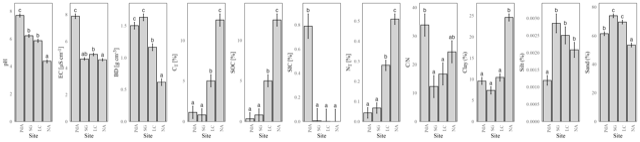
\includegraphics[width=1\textwidth]{img/baseline_by_site.png}
    % The caption remains the same
    \caption{Soil physical and chemical properties across the four study sites (PdA: Pan de Azúcar, SG: Santa Gracia, LC: La Campana, and NA: Nahuelbuta). Letter-based display accompanying soil properties with significant effect for site. Different letters indicate statistically significant differences ($p < 0.05$, Šidák correction).}
    % The label remains the same
    \label{fig:baseline_site}
\end{sidewaysfigure}

\FloatBarrier

\subsection{Biocrust-induced changes in soil properties}
\label{sec:BicorustInducedSoil}

Biocrust presence significantly ($p < 0.05$) influenced several soil properties (Figure \ref{fig:baseline_biocrust_interaction}a), often interacting with the climatic site (Figure \ref{fig:baseline_biocrust_interaction}b). A significant site $\times$ biocrust interaction was observed for bulk density, with biocrusts associated with a decrease in BD in arid PdA but an increase in Mediterranean LC. Biocrust presence significantly affected soil texture overall, associated with a slight decrease in clay and an increase in silt content when averaged across sites. However, the site $\times$ biocrust interaction was significant for clay, showing a notable increase under biocrusts specifically in PdA. Across all sites, biocrust presence led to a small but statistically significant decrease in soil pH, potentially reflecting localized acidification due to respiration \citep{Bachar2010}. C\textsubscript{T} and SOC contents were significantly lower under biocrusts when averaged across all sites. A significant site $\times$ biocrust interaction affected N\textsubscript{T}, showing significantly lower values under biocrusts only in the humid LC and NA sites. The C/N ratio was significantly lower under biocrusts overall, driven partly by changes in PdA. Electrical conductivity (EC) was extremely high in PdA compared to other sites, and the site $\times$ biocrust interaction showed a significant reduction in EC under biocrusts only in PdA.

% I will include it sideways for better visualization
\begin{sidewaysfigure}
    \centering
    % The \includegraphics command remains the same
    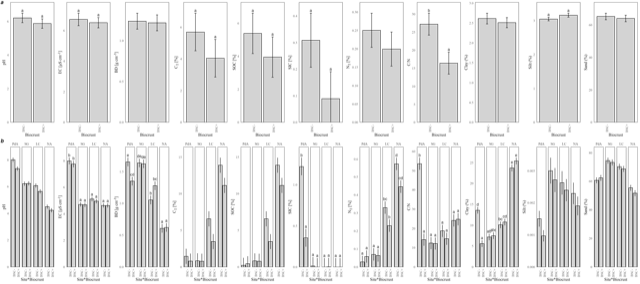
\includegraphics[width=1\textwidth]{img/baseline_by_biocrust_interaction.png}
    % The caption remains the same, clean up the p<0.05 part
    \caption{Biocrust (a) and interaction (b) effects on soil properties. Soil physical and chemical properties across for biocrust (BSC+ vs. BSC-) and the interaction with the site (PdA: Pan de Azúcar, SG: Santa Gracia, LC: La Campana, and NA: Nahuelbuta). Letter-based display accompanying soil properties with significant effect for site or site*biocrust. Different letters indicate statistically significant differences ($p < 0.05$, Šidák correction).} % Use math mode for p < 0.05
    % The label remains the same
    \label{fig:baseline_biocrust_interaction}
\end{sidewaysfigure} % *** End sidewaysfigure environment ***

\FloatBarrier

\subsection{Biocrust and climate interactions on aggregate stability}
\label{sec:BiocrusClimateInducedSoil}

Soil aggregate stability showed clear responses to both the climatic gradient and biocrust cover, particularly when assessed under wet conditions. Overall aggregate stability, indicated by the difference in geometric mean diameter ($\Delta$GMD), significantly increased (lower $\Delta$GMD indicates higher stability) along the climatic gradient from PdA (mean $\Delta$GMD \SI{1.86}{\milli\meter}) to NA (mean $\Delta$GMD \SI{0.83}{\milli\meter}), although SG showed higher stability (mean $\Delta$GMD \SI{1.2}{\milli\meter}) than LC (mean $\Delta$GMD \SI{1.4}{\milli\meter}). The water stability aggregate ratio (WSAR) confirmed this trend, with NA (mean WSAR 81.1\%) being significantly more stable than the other sites (mean WSAR 57.7\% - 73.4\%).

Biocrusts exerted a significant stabilizing effect, particularly on larger aggregates under wet sieving conditions. The presence of biocrusts significantly increased the proportion of water-stable aggregates $>$\SI{2}{\milli\meter} overall. Specifically, the interaction between site and biocrust was significant for wet aggregates in the \SIrange[range-phrase=--,range-units=single]{9.5}{30.0}{\milli\meter} range, showing a stabilizing effect (increase in proportion) in PdA, SG, and LC, but not in the humid NA site. This suggests a threshold effect, where the stabilizing role of biocrusts diminishes as vascular vegetation and associated stabilizing agents become more dominant under humid conditions. Correspondingly, biocrust presence significantly decreased the proportion of water-stable aggregates $<$\SI{2}{\milli\meter} (R\textsubscript{$<$\SI{2}{\milli\meter}}) overall (from mean 63.7\% without biocrusts to 57.5\% with biocrusts) (Figure \ref{fig:aggregate-stability}).

These findings highlight that biocrusts contribute to soil structure by binding particles and microaggregates, likely through mechanisms involving fungal hyphae, cyanobacterial filaments, and the production of extracellular polymeric substances \citep{Six2004,Totsche2018}. While biocrusts influenced bulk C and N contents, the lack of a direct correlation between these bulk changes and stability across all sites suggests that the specific composition and micro-spatial arrangement of organic binding agents within aggregates, rather than just total C or N, are critical for stability \citep{Wagner2007}. The results emphasize the crucial role of biocrusts as primary stabilizing agents in arid and semi-arid ecosystems \citep{BelnapBudel2016}, with their influence gradually yielding to vascular plants and associated soil organic matter dynamics in more humid environments.

\begin{figure}[h!]
	\centering
	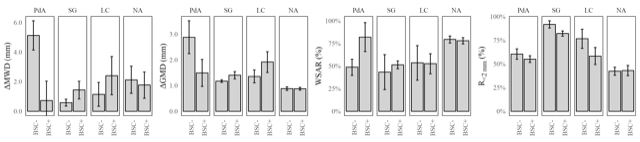
\includegraphics[width=1\textwidth]{img/aggregate stability indexes_se.png}
	\caption{Aggregate stability indexes for Pan de Azúcar (PdA), Santa Gracia (SG), La Campana (LC), and Nahuelbuta (NA) for biocrust (BSC+) and non-biocrust (BSC-) treatments displayes as mean and standard error. $\Delta$MWD: difference in mean weight diameter, $\Delta$GMD: difference in geometric mean diameter, WSAR: water stability aggregate ratio, R$_{<\SI{2}{\milli\meter}}$: ratio of aggregates less than \SI{2}{\milli\meter}.}
	\label{fig:aggregate-stability}
\end{figure}
\FloatBarrier


\section[Effect of biocrust on water flow, erosion and nutrient flow]{Effect of biocrust on water flow, erosion and nutrient flow (manuscript 2)}
\label{sec:BiocrustOnFlows}

This study investigated the role of biological soil crusts (biocrusts) as climate-dependent regulators of erosion, water, and nutrient cycling using rainfall simulation experiments across a 910 km climate gradient in the Coastal Mountain Range of Chile. Four study sites represented coastal semi-arid (SG), inland semi-arid (QdT), Mediterranean (LC), and humid (NA) climates. These sites, characterized by comparable topography and granitic parent material, allowed for assessing biocrust influence under varying climatic conditions by comparing undisturbed soil monoliths with (+) and without (-) biocrust cover. We analyzed surface runoff, percolation flow, sediment transport, and associated carbon (C) and nitrogen (N) fluxes.

Soil properties varied across the climate gradient, reflecting differing weathering intensities and soil development stages relevant to hydrological and erosion responses. Notably, the inland semi-arid site (QdT) exhibited high biocrust cover despite lower water availability compared to the coastal SG site, likely due to protection from disturbance within a fenced area since 2011, fostering biocrust development \citep{Budel2016}. Soil texture across sites was predominantly sandy loam, with clay content increasing southward, influencing water retention and infiltration pathways.

\subsection{Biocrust influence on water flow and sediment transport}
\label{sec:BiocrustOnWaterSesimentsFlows}

Biocrusts significantly modulated water flow and erosion dynamics, though their effects varied with climate and the specific pathway (runoff vs. percolation). Regarding runoff dynamics (Table \ref{tab:runoff_fluxes}), biocrusts delayed runoff initiation across all sites, with a mean delay of 97.7\%. This effect was particularly noticeable at the humid NA site, where dense bryophyte cover increased surface roughness and water storage \citep{Kidron2022}. Overall, biocrusts reduced total runoff volume by an average of 28.0\%, although this was site-specific, ranging from a 72.4\% reduction in NA to an unexpected 36.4\% increase in LC. Despite these impacts on surface flow, biocrusts did not measurably affect the time required for percolation to commence (Table \ref{tab:percolation_fluxes}). The reduction in runoff volume (Table \ref{tab:runoff_fluxes}) coupled with unchanged percolation timing (Table \ref{tab:percolation_fluxes}) indicated enhanced cumulative infiltration and saturated hydraulic conductivity in the presence of biocrusts compared to bare soil. In terms of erosion and sediment flux, biocrusts proved highly effective at reducing soil erosion via surface runoff, decreasing total sediment transport by an average of 69.9\% and sediment concentration in runoff by 60.9\% (Table \ref{tab:runoff_fluxes}). The most significant reduction occurred at the inland semi-arid QdT site, highlighting the protective role of biocrusts  \citep{RodriguezCaballero2018}. Conversely, sediment mobilization via percolation increased by 28.3\%, and sediment concentration in percolation rose by 58.3\% when biocrusts were present. This demonstrates a clear shift in sediment transport dynamics, moving from predominantly surface erosion on bare soil to increased subsurface transport under biocrust cover.

\begin{sidewaystable} % Using sidewaystable instead of table
    % \centering % Centering is often implicit/less relevant for full-page sideways tables
    \begin{threeparttable}
        \caption{Surface runoff fluxes on the study sites (SG: Santa Gracia, QdT: Quebrada de Talca, LC: La Campana, NA: Nahuelbuta) with (+) and without (-) biocrust (BSC) cover. Values correspond to mean $\pm$ standard deviation (SD) of five field replicates. Different letters indicate statistically significant different values based on Šidák correction post-hoc test results.}
        \label{tab:runoff_fluxes}

        % Define column widths/types. S columns align numbers. 'l' for text.
        % Determine table-format based on max digits before/after decimal, plus uncertainty.
        \begin{tabular}{@{} ll S[table-format=3.1(3.1)] l % Time
                             S[table-format=2.0(2.0)] l % Runoff
                             S[table-format=3.0(3.0)] l % Sediment
                             S[table-format=2.1(2.1)] l % Sed. Load
                       @{}}
            \toprule
            % --- Headers ---
            % Using \makecell for multi-line headers with units
            \multicolumn{2}{@{}l}{\textbf{Factor}} % Span first two columns for header alignment
            & \multicolumn{2}{c}{\makecell{\textbf{Time to start runoff}\tnote{a}\\ {[\si{\second}]}}}
            & \multicolumn{2}{c}{\makecell{\textbf{Runoff}\tnote{a}\\ {[\si{\liter\per\hour}]}}}
            & \multicolumn{2}{c}{\makecell{\textbf{Sediment in runoff}\tnote{a}\\ {[\si{\gram\per\meter\squared\per\hour}]}}}
            & \multicolumn{2}{c}{\makecell{\textbf{Sediment load of runoff}\tnote{a}\\ {[\si{\gram\per\liter\per\meter\squared}]}}} \\
            \cmidrule(lr){3-4} \cmidrule(lr){5-6} \cmidrule(lr){7-8} \cmidrule(lr){9-10} % Rules under spanned headers

            % --- Data Rows ---
            % Mean Site Effects
            Mean $\pm$ SD & SG   & 65.1 \pm 20.7  & (a) & 49 \pm 18  & (b) & 617 \pm 473 & (c) & 12.1 \pm 7.9  & (a) \\
                          & QdT  & 78.7 \pm 30.4  & (a) & 40 \pm 16  & (a) & 398 \pm 459 & (b) & 9.6 \pm 9.6   & (a) \\
                          & LC   & 83.5 \pm 56.0  & (a) & 39 \pm 22  & (a) & 241 \pm 293 & (b) & 7.3 \pm 8.8   & (a) \\
                          & NA   & 236.7 \pm 273.0& (b) & 44 \pm 43  & (a) & 28 \pm 44   & (a) & 3.0 \pm 14.0  & (a) \\
            \midrule
            % Mean Biocrust Effects
            Biocrust      & BSC+ & 154.0 \pm 211.5& (b) & 36 \pm 21  & (a) & 149 \pm 222 & (a) & 4.5 \pm 10.4  & (a) \\
                          & BSC- & 77.9 \pm 33.8  & (a) & 50 \pm 31  & (b) & 495 \pm 492 & (b) & 11.5 \pm 10.0 & (b) \\
            \midrule
            % Interaction Effects
            Site*Biocrust & SG BSC+ & 62.7 \pm 21.2 & (ab) & 44 \pm 16 & (ab) & 340 \pm 340 & (bc)  & 7.5 \pm 5.7  & (abc)  \\
                          & SG BSC- & 67.5 \pm 20.6 & (ab) & 54 \pm 18 & (ab) & 873 \pm 456 & (d)   & 16.7 \pm 7.1 & (de)   \\ \addlinespace
                          & QdT BSC+& 87.3 \pm 37.5 & (ab) & 38 \pm 15 & (ab) & 131 \pm 96  & (ab)  & 3.3 \pm 2.0  & (abd)  \\
                          & QdT BSC-& 70.1 \pm 18.7 & (ab) & 42 \pm 18 & (ab) & 665 \pm 524 & (cd)  & 15.8 \pm 10.2& (ce)   \\ \addlinespace
                          & LC BSC+ & 85.8 \pm 67.1 & (ab) & 45 \pm 20 & (ab) & 87 \pm 94   & (a)   & 2.1 \pm 1.9  & (a)    \\
                          & LC BSC- & 81.2 \pm 44.6 & (ab) & 33 \pm 23 & (ab) & 395 \pm 344 & (bc)  & 12.6 \pm 9.9 & (bcde) \\ \addlinespace
                          & NA BSC+ & 380.4 \pm 329.5& (b) & 19 \pm 23 & (a)  & 16 \pm 49   & (a)   & 5.2 \pm 19.9 & (abcde)\\
                          & NA BSC- & 93.0 \pm 40.2 & (a) & 69 \pm 45 & (b)  & 40 \pm 36   & (a)   & 0.9 \pm 1.2  & (abcde)\\
            \bottomrule
        \end{tabular}

        % --- Table Notes ---
        \begin{tablenotes}[para,flushleft] % para puts notes on one line if space, flushleft aligns note markers
           \item[a] Letter-based display accompanying surface runoff parameters. Different letters within a column section (Mean, Biocrust, or Site*Biocrust interaction) indicate statistically significant differences ($p < 0.05$, Šidák correction).
        \end{tablenotes}

    \end{threeparttable}
\end{sidewaystable} % *** End the sidewaystable environment ***


\begin{sidewaystable} % Using sidewaystable for landscape orientation
    \begin{threeparttable}
        \caption{Percolating water fluxes on the study sites (SG: Santa Gracia, QdT: Quebrada de Talca, LC: La Campana, NA: Nahuelbuta) with (+) and without (-) biocrust (BSC) cover. Values correspond to mean $\pm$ standard deviation (SD) of five field replicates. Different letters indicate statistically significant different values based on Šidák correction post-hoc test results.}
        \label{tab:percolation_fluxes} % Unique label for this table

        % Use tabular* to fill the linewidth.
        % Column structure MUST match Table 2: ll Sl Sl Sl Sl
        % Add 'l' columns even where no letters exist in Table 3.
        \begin{tabular*}{\linewidth}{@{\extracolsep{\fill}} % Distribute extra space
                             ll % Factor Column 1 & 2 (left aligned)
                             @{\extracolsep{\fill}} % Space after Factor columns
                             S[table-format=3.0(3.1)] l % Time Column 3 (S) + EMPTY Letter Column 4 (l)
                             @{\extracolsep{\fill}} % Space after Time group
                             S[table-format=2.1(2.0)] l % Percolation Column 5 (S) + Letter Column 6 (l)
                             @{\extracolsep{\fill}} % Space after Percolation group
                             S[table-format=2.0(2.0)] l % Sediments Column 7 (S) + Letter Column 8 (l)
                             @{\extracolsep{\fill}} % Space after Sediments group
                             S[table-format=1.1(2.1)] l % Sed. Load Column 9 (S) + EMPTY Letter Column 10 (l)
                             @{} % No padding at the end
                             }
            \toprule
            % --- Headers ---
            % Span 2 columns (S+l) for EACH parameter header for consistent layout
            \multicolumn{2}{@{}l}{\textbf{Factor}}
            & \multicolumn{2}{c}{\makecell{\textbf{Time to start}\\\textbf{percolation flow}\\ {[\si{\second}]}}}
            & \multicolumn{2}{c}{\makecell{\textbf{Percolation}\tnote{a}\\ {[\si{\liter\per\hour}]}}}
            & \multicolumn{2}{c}{\makecell{\textbf{Sediments in}\\\textbf{percolation flow}\tnote{a}\\ {[\si{\gram\per\meter\squared\per\hour}]}}}
            & \multicolumn{2}{c}{\makecell{\textbf{Sediment load in}\\\textbf{percolation}\\ {[\si{\gram\per\liter\per\meter\squared}]}}} \\
            % cmidrules span 2 cols each, matching headers
             \cmidrule(lr){3-4} \cmidrule(lr){5-6} \cmidrule(lr){7-8} \cmidrule(lr){9-10}

            % --- Data Rows ---
            Mean $\pm$ SD & SG   & \num{223 \pm 190}   &     & \num{18.0 \pm 14}  & (a) & \num{19 \pm 34} &     & \num{4.2 \pm 19.7} &   \\
                          & QdT  & \num{175.0 \pm 94.5}&     & \num{22.8 \pm 15}  & (a) & \num{7 \pm 10}  &     & \num{0.2 \pm 0.3}  &   \\
                          & LC   & \num{234 \pm 183}   &     & \num{22.4 \pm 13}  & (a) & \num{13 \pm 15} &     & \num{0.5 \pm 0.5}  &   \\
                          & NA   & \num{145 \pm 169}   &     & \num{65.0 \pm 39}  & (b) & \num{23 \pm 25} &     & \num{0.4 \pm 0.4}  &   \\
            \midrule
            Biocrust      & BSC+ & \num{171 \pm 133}   &     & \num{42.6 \pm 34}  & (b) & \num{19 \pm 22} & (b) & \num{0.5 \pm 0.5}  &   \\
                          & BSC- & \num{218 \pm 190}   &     & \num{21.5 \pm 21}  & (a) & \num{12 \pm 24} & (a) & \num{2.1 \pm 13.7} &   \\
            \midrule
            Site*Biocrust & SG BSC+  & \num{202 \pm 103}   &     & \num{24.8 \pm 15}  & (ab) & \num{19 \pm 18} &     & \num{0.7 \pm 0.5}  &   \\
                          & SG BSC-  & \num{244 \pm 251}   &     & \num{11.1 \pm 10}  & (a)  & \num{18 \pm 46} &     & \num{7.5 \pm 27.5} &   \\ \addlinespace
                          & QdT BSC+ & \num{148.0 \pm 63.9}&     & \num{30.5 \pm 13}  & (b)  & \num{9 \pm 13}  &     & \num{0.3 \pm 0.3}  &   \\
                          & QdT BSC-& \num{202 \pm 113}   &     & \num{15.1 \pm 13}  & (ab) & \num{5 \pm 6}   &     & \num{0.2 \pm 0.2}  &   \\ \addlinespace
                          & LC BSC+  & \num{226 \pm 223}   &     & \num{23.5 \pm 14}  & (ab) & \num{17 \pm 19} &     & \num{0.6 \pm 0.5}  &   \\
                          & LC BSC-  & \num{241 \pm 139}   &     & \num{21.3 \pm 14}  & (ab) & \num{9 \pm 9}   &     & \num{0.4 \pm 0.3}  &   \\ \addlinespace
                          & NA BSC+  & \num{107.0 \pm 35.6}&     & \num{91.5 \pm 28}  & (c)  & \num{30 \pm 32} &     & \num{0.4 \pm 0.4}  &   \\
                          & NA BSC-  & \num{183 \pm 234}   &     & \num{38.5 \pm 30}  & (b)  & \num{16 \pm 15} &     & \num{0.4 \pm 0.3}  &   \\

            \bottomrule
        \end{tabular*} % End tabular*

        % --- Table Notes ---
        \begin{tablenotes}[para,flushleft]
           \item[a] Letter-based display accompanying parameters where shown. Different letters within a column section (Mean, Biocrust, or Site*Biocrust interaction) indicate statistically significant differences ($p < 0.05$, Šidák correction).
        \end{tablenotes}

    \end{threeparttable}
\end{sidewaystable} % End the sidewaystable environment

\FloatBarrier

\FloatBarrier

\subsection{Biocrust modulation of carbon and nitrogen fluxes}
\label{sec:BiocrustOnNutrientFlows}

Biocrusts significantly altered the transport pathways and amounts of C and N in both sediment-bound and dissolved forms, with effects dependent on climate and site conditions (Figure \ref{fig:nutrient-flow}). For carbon fluxes, sediment-associated C loss via runoff generally increased with climatic humidity. Biocrusts significantly reduced this sediment C loss, by up to a factor of four compared to bare soil. In percolation flow, biocrusts also reduced the C content in mobilized sediments, an effect most pronounced in drier climates where reductions reached 20-40\%. Furthermore, biocrusts consistently increased dissolved organic carbon (DOC) concentrations in runoff across all sites, suggesting an alteration of C cycling pathways towards leaching rather than just physical erosion \citep{Baumert2021}. Similar patterns, though moderated by site*biocrust interactions, were observed for DOC transported via percolation. Regarding nitrogen fluxes, sediment-associated N loss via runoff also increased with humidity. The biocrust effect on this sediment N was strongly site-specific, causing an increase in SG but a decrease in NA, and explaining 48.8\% of the observed variability. Dissolved organic nitrogen (DON) fluxes in runoff showed trends analogous to DOC, generally increasing with biocrust presence, especially in northern sites like SG (increasing from 1.3$\pm$1.0 ppm in BSC- to 2.2$\pm$2.0 ppm in BSC+). However, a contrasting effect was observed at the humid NA site, where biocrusts decreased DON in runoff (from 0.6$\pm$0.7 ppm in BSC- to 0.3$\pm$0.8 ppm in BSC+), potentially indicating enhanced N immobilization or uptake in this N-richer ecosystem. DON fluxes transported via percolation followed similar site-dependent trends influenced by biocrust interactions.

\begin{figure}[h!]
	\centering
	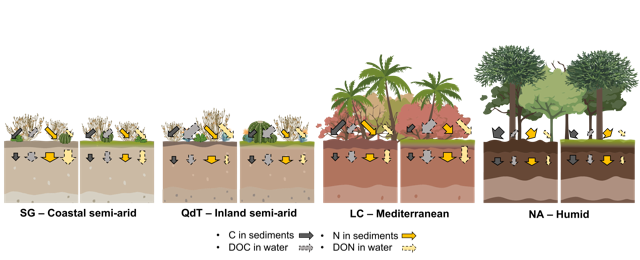
\includegraphics[width=1\textwidth]{img/nutrient-flow-diagram.png}
	\caption{Representation of total carbon in sediments and DOC in water fluxes for the four study sites. The diagrams at the right side with slightly green surface represents the BSC+ treatments and the one at the left the BSC-. Grey-filled arrows correspond to C fluxes, and yellowish arrows to N. At the same time, arrows with solid borders correspond to the flow attached to the sediments, and dashed arrows dissolved in water. Each type of arrow is proportional inside each group in width to the concentration of nutrients and in length to the mass of it.}
	\label{fig:nutrient-flow}
\end{figure}

\FloatBarrier

Overall, biocrusts play a crucial, climate-dependent role in regulating water flow, significantly reducing surface runoff erosion, but potentially increasing subsurface sediment transport. They profoundly influence C and N cycling, generally reducing C losses via runoff while altering dissolved nutrient pathways, with specific effects on N mobilization varying strongly between arid and humid environments.

\section[Microbial, plant and moisture controls on soil structure and functionality]{Microbial, plant and moisture controls on soil structure and functionality (manuscripts 3, 4 and 5)}
\label{sec:MicrobesPlantsMoistureStructure}

Beyond the direct impacts of biological soil crusts (BSCs) and the broad climatic gradient, further investigations using subsets of the study sites (primarily arid Pan de Azúcar (PdA) and semi-arid Santa Gracia (SG), but also including mediterranean La Campana (LC) and humid Nahuelbuta (NA) in Manuscript 4) provided deeper insights into the roles of the indigenous microbial community, plant roots, and moisture dynamics in shaping soil aggregation, organic matter turnover, and nutrient cycling. These studies employed controlled laboratory incubations simulating specific scenarios: a shift to humid conditions for arid/semi-arid soils (Manuscript 3), repeated wetting-drying (W-D) versus constant moisture (CM) regimes across the climate gradient (Manuscript 4), and the natural transition from a living rhizosphere to a decomposing detritusphere in semi-arid soil (Manuscript 5).

A central finding emerging from these experiments is that the impact of microbial activity on soil aggregation and related properties is highly dependent on the origin of the soil and the prevailing environmental conditions. This was clearly demonstrated in the moisture regime experiment (Manuscript 4), where the responses of native, microbially active soils to repeated wetting-drying (W-D) cycles were compared against sterilized controls across the climate gradient. Principal Component Analysis visually distinguished the trajectories of native versus sterile soils under W-D stress, directly highlighting the significant contribution of microbial activity to changes in soil edaphic properties (Figure \ref{fig:PCA-microbes}). Crucially, the nature of this microbial influence differed markedly between climate zones. In arid soils, the microbially-influenced samples were primarily characterized by changes in aggregate C/N ratios, suggesting accelerated turnover of labile organic matter (OM) fueled by the Birch effect (Figure \ref{fig:PCA-microbes}A). In contrast, microbially-influenced semi-arid and mediterranean soils under W-D were distinguished from controls mainly by shifts in aggregate size distribution, particularly an increase in microaggregates (MIC) relative to macroaggregates (MAC) (Figure \ref{fig:PCA-microbes}B-C). This direct comparison underscores that while microbes actively mediate soil structural changes during moisture fluctuations, the specific mechanisms and outcomes (OM turnover vs. aggregate reorganization) are strongly dictated by the climate legacy imprinted on the soil and its microbial community.

\begin{figure}[h!]
	\centering
	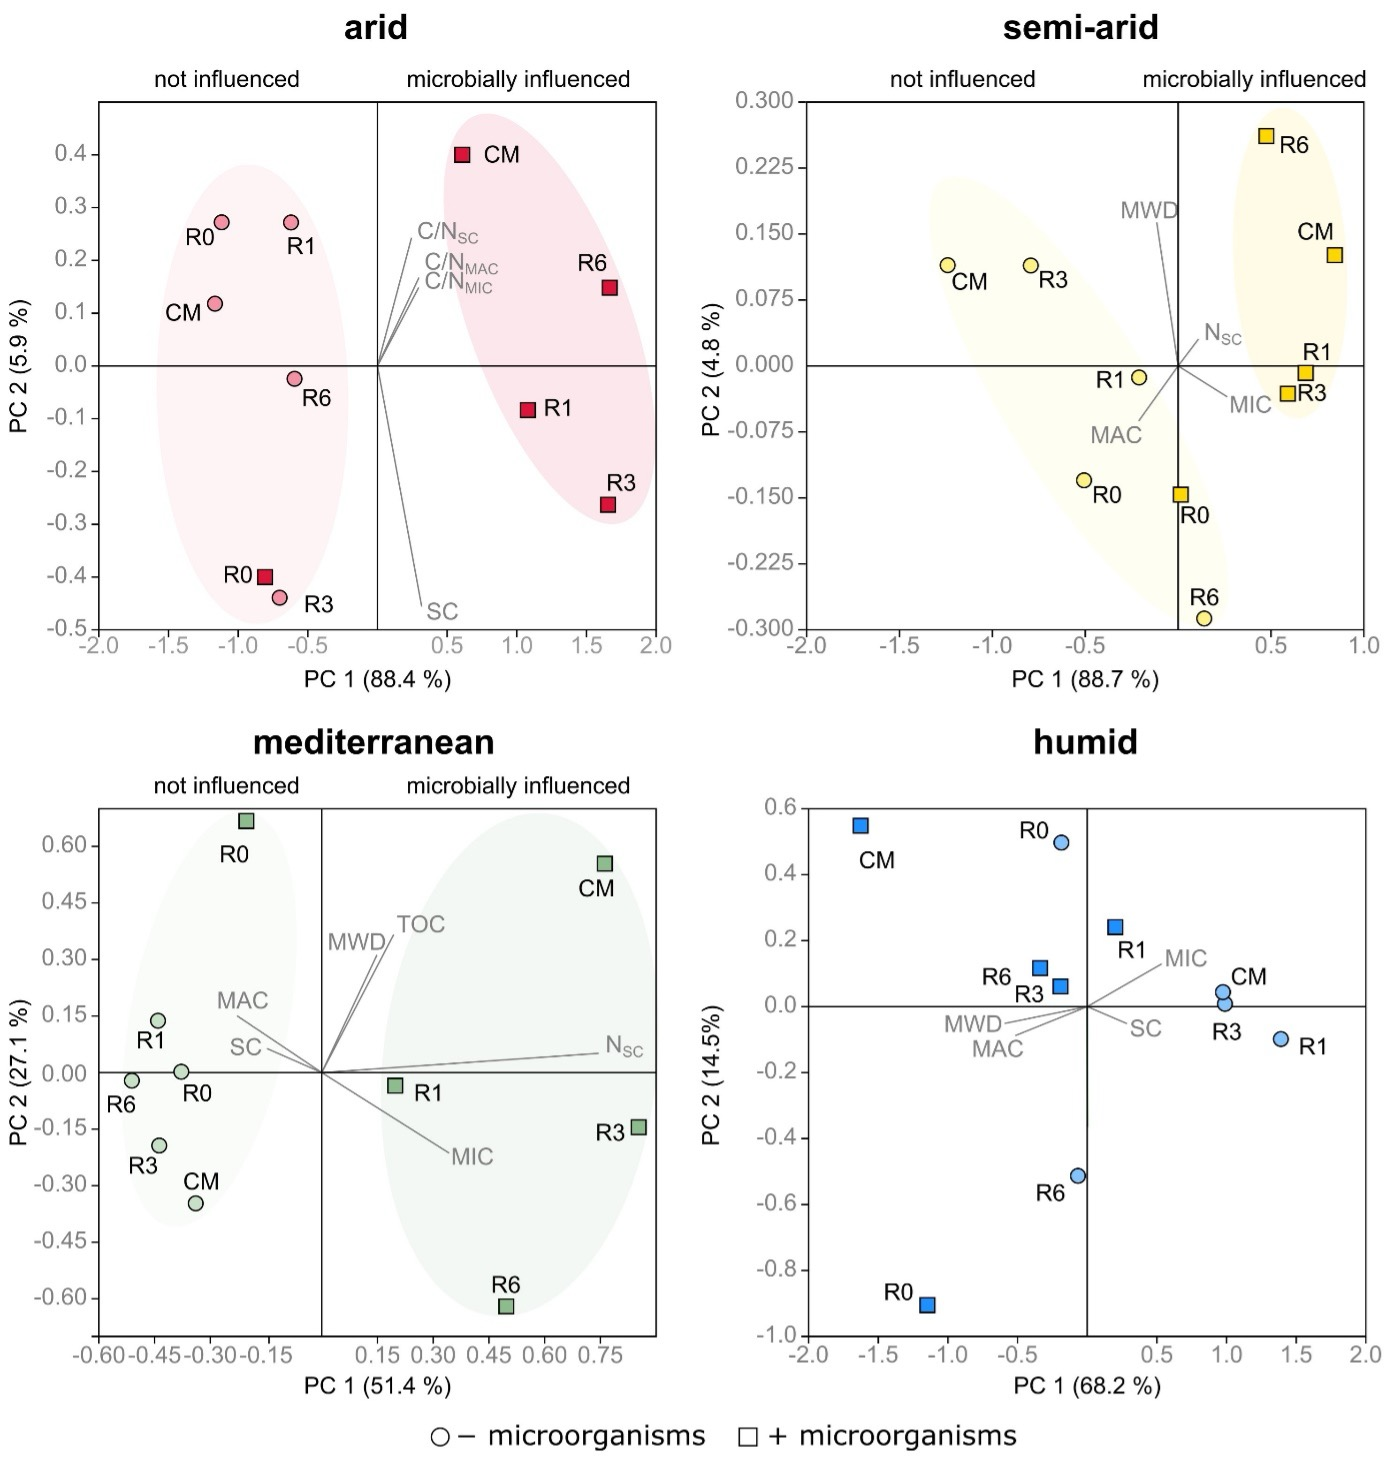
\includegraphics[width=1\textwidth]{img/PCA-microbes-structure.jpg}
	\caption{Principal Component Analyses of soil properties in native soils (squares) and sterilized soils (circles) including significant soil properties. A) arid, B) semi-arid, C) mediterranean and D) humid site. Microbial influence is indicated by sample separation along the x-axis.}
	\label{fig:PCA-microbes}
\end{figure}

\FloatBarrier

Further results support this picture of context-dependent microbial influence and climate legacy effects. The observed increase in aggregate C/N ratios in microbially active arid soils (Figure \ref{fig:bacterial-abundance}A) aligns with findings of stimulated microbial abundance under W-D but also a net breakdown of MAC and only a slight decrease in overall aggregate stability (MWD) (Manuscript 4), consistent with rapid consumption of labile OM released from decomposing larger aggregates. The microaggregate formation observed in microbially influenced semi-arid and mediterranean soils (Figure \ref{fig:PCA-microbes}B-C) corresponds with outcomes where overall stability either slightly decreased (semi-arid) or increased (mediterranean) (Manuscript 4), suggesting different stabilization pathways potentially involving OM redistribution or transformation.

\begin{figure}[h!]
	\centering
	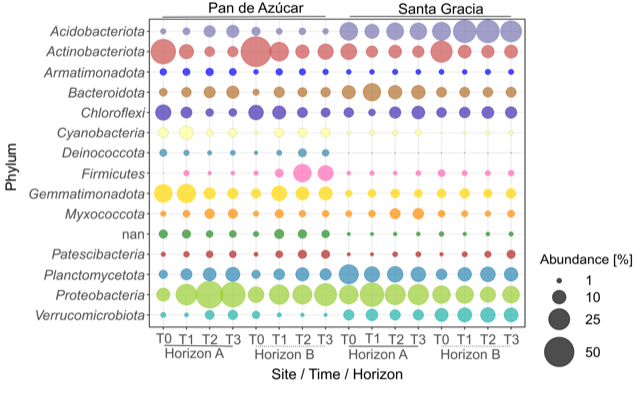
\includegraphics[width=1\textwidth]{img/bacterial-abundance.png}
	\caption{Relative abundance of top 15 bacterial phyla for Pan de Azúcar and Santa Gracia and the different time points. Time is represented as T0 (original), T1 (2 weeks), T2 (12 weeks) and T3 (16 weeks). Each bubble is the mean of the different treatments (in situ, BSCs and plants) and technical triplicates.}
	\label{fig:bacterial-abundance}
\end{figure}

\FloatBarrier

The importance of climate legacy was also evident in the differential resilience of microbial communities themselves. The arid PdA community, adapted to stable hyperaridity, showed significant structural changes and diversity loss under simulated humid conditions (Manuscript 3), while the semi-arid SG community, from a more variable climate, demonstrated greater stability (Figure \ref{fig:bacterial-abundance}), mirroring the patterns observed in the PCA analysis (Figure \ref{fig:PCA-microbes}).

Beyond the intrinsic microbial community and moisture effects, the powerful role of plants was confirmed (Manuscript 5). Living roots acted as potent drivers of macroaggregation in both topsoil and subsoil of semi-arid origin. However, a distinct root legacy effect was apparent, as this enhanced aggregation only persisted after plant death in the topsoil, indicating a requirement for continuous C input or greater inherent stability factors in the subsoil. This transition from rhizosphere to detritusphere also drove a microbial succession from fungal to Gram-positive bacterial dominance and altered OM protection mechanisms, notably increasing occluded POM in the topsoil detritusphere.

\chapter{Conclusion \& Outlook}

This research investigated the multifaceted role of biological soil crusts (biocrusts) and microbial communities in shaping soil development, stability, and nutrient cycling across a climate gradient in the Chilean Coastal Range. By combining field observations, laboratory experiments, and advanced analytical techniques, this work provides valuable insights into the complex interactions between biota, climate, and soil processes.

A key focus of this research was to understand the influence of biocrusts on soil aggregate stability and their interplay with soil properties along a climate gradient. Four sites representing arid, semi-arid, Mediterranean, and humid conditions were selected, allowing for a comparative analysis of biocrust effects under contrasting environmental conditions. The results revealed significant variations in soil properties along the gradient, with bulk density decreasing and soil organic carbon (SOC), total nitrogen (N\textsubscript{T}), and clay content increasing with humidity. These variations reflect the influence of climate on weathering processes, organic matter accumulation, and soil development \cite{Jenny1941}. Biocrust cover significantly influenced soil properties, particularly in arid and semi-arid sites, where it increased SOC and N\textsubscript{T} content and altered soil texture, indicating its role in trapping organic matter and modifying soil structure \citep{Belnap2003,Bowker2006}. Aggregate stability, a key indicator of soil resilience to erosion, was enhanced by the presence of biocrusts across all climates, with the most pronounced effect observed in the arid site. This finding underscores the crucial role of biocrusts in protecting vulnerable soils in dryland environments \citep{Chamizo2012}. The difference in geometric mean diameter of aggregates further emphasized the stabilizing effect of biocrusts, particularly in the arid site, where they significantly increased aggregate size.

Extending the investigation of biocrusts beyond their impact on soil structure, this research also explored their role as climate-dependent regulators of erosion, water, and nutrient cycling. Utilizing rainfall simulation experiments across the same climate gradient, the study assessed the effects of biocrusts on surface runoff, percolation flow, and sediment and nutrient fluxes. Biocrusts significantly delayed the initiation of runoff and reduced overall runoff volume in all climates, highlighting their capacity to retain water and mitigate erosion \citep{Kidron2022}. The influence of biocrusts on sediment discharge was equally pronounced, with significant reductions observed across all sites, particularly in the inland semi-arid environment. Furthermore, biocrusts influenced both sediment-bound and dissolved carbon and nitrogen dynamics, with contrasting effects observed across the climate gradient. While biocrusts increased carbon content in sediments mobilized by runoff at drier sites, they also enhanced dissolved organic carbon (DOC) concentrations, indicating alterations in carbon cycling pathways. Similarly, biocrusts influenced nitrogen fluxes, increasing dissolved organic nitrogen (DON) concentrations, but with varying effects across the climatic gradient. These findings underscore the complex and context-dependent role of biocrusts in regulating both hydrological and biogeochemical processes in soil ecosystems.

Complementing the field and rainfall simulation studies, laboratory experiments explored the microbial drivers of soil aggregate turnover across different climates and moisture regimes. By subjecting soils from the same climate gradient sites to controlled wetting-drying (W-D) cycles, this research aimed to dissect the relative contributions of abiotic and biotic factors in shaping soil structure. The results revealed distinct patterns in aggregate size distribution and stability across climates and in response to W-D cycles. Sterilization significantly altered aggregate dynamics, highlighting the crucial role of microbial communities in soil structure formation and stabilization \citep{Six2004}. Microbial abundance, diversity, and community composition also exhibited climate-specific responses to W-D cycles, reflecting the adaptive strategies of soil microorganisms to fluctuating moisture conditions. W-D cycles also impacted predicted microbial functions, influencing the decomposition of organic matter and nutrient cycling processes.

Building upon the findings related to microbial influence on soil aggregate dynamics, the research further explored the role of microbial communities in initial soil formation under simulated climate change scenarios. Using soil samples from arid and semi-arid sites, the study simulated increased humidity conditions, reflecting potential climate change projections for these regions. The results revealed significant shifts in microbial community structure and function in response to the simulated climate change, with certain microbial groups, notably Sphingomonas, exhibiting increased abundance and potential for nitrogen fixation. These findings underscore the importance of soil legacy effects and the potential for microbial communities to adapt and mediate soil processes under changing environmental conditions.

Lastly, the research delved into the specific role of roots in regulating soil aggregation and organic matter dynamics, focusing on the transition from rhizosphere to detritusphere. Microcosm experiments with living and decaying cereal roots revealed significant differences in soil aggregate formation, microbial community composition, and organic matter characteristics. Living roots promoted the development of macroaggregates, particularly in the subsoil, while decaying roots stimulated microbial activity and altered organic matter decomposition pathways. These findings emphasize the dynamic interplay between living and decaying roots and their influence on soil structure, microbial communities, and organic matter cycling. The transition from rhizosphere to detritusphere represents a shift from root-driven soil formation to decomposition-dominated processes, highlighting the interconnectedness of plant and microbial contributions to soil ecosystem functioning.

In summary, this body of research demonstrates the complex and interconnected roles of biocrusts, microbial communities, and plant roots in shaping soil development, stability, and nutrient cycling across a climate gradient. Biocrusts act as key regulators of surface processes, enhancing soil aggregate stability, reducing erosion, and modulating water and nutrient fluxes. Microbial communities, as the engines of biogeochemical processes, drive soil aggregation, organic matter decomposition, and respond dynamically to changes in moisture availability and climate conditions. Plant roots, both living and decaying, influence soil structure formation, microbial communities, and organic matter dynamics, with distinct effects observed in rhizosphere and detritusphere environments.

Future research should focus on further disentangling the complex interactions between biocrusts, microbial communities, and plants. This includes investigating the specific mechanisms driving biocrust formation and their influence on different soil types, exploring the functional diversity of microbial communities involved in soil aggregate formation, and examining the long-term legacy effects of plant-soil interactions on soil carbon sequestration. Moreover, considering the projected impacts of climate change, future studies should assess the resilience of biocrusts and microbial communities to altered precipitation patterns, temperature regimes, and increased atmospheric $CO_2$ concentrations. By deepening our understanding of these complex interactions, we can develop more effective strategies for soil conservation, ecosystem management, and promoting the sustainable use of soil resources in the face of global environmental change.


% --- Main Bibliography ---

\bibliographystyle{natbib} % Consider changing to a style compatible with KOMA/natbib if issues arise
\bibliography{literatur_all_clean}

\appendix % Start the appendix environment

% --- Code to Suppress Appendix Chapter Titles on First Page ---
\makeatletter % Need access to internal KOMA commands

% Store the original definitions
\let\originalchapterlinesformat\chapterlinesformat
\let\originalchapterlineswithprefixformat\chapterlineswithprefixformat

% Redefine the commands to do nothing *only for chapters*
% This prevents the "Appendix A: Title" text from being printed on the page
\renewcommand{\chapterlinesformat}[3]{%
    \ifstr{#1}{chapter}{% Check if the sectioning level is 'chapter'
        % If it IS a chapter, do nothing to suppress the heading on the page
        \@afterindentfalse % Standard KOMA internal setting
        \@afterheading     % Standard KOMA internal command
    }{% If it's NOT a chapter (e.g., part), use the original command
        \originalchapterlinesformat{#1}{#2}{#3}%
    }%
}
\renewcommand{\chapterlineswithprefixformat}[4]{%
     \ifstr{#1}{chapter}{% Check if the sectioning level is 'chapter'
        % If it IS a chapter, do nothing to suppress the heading on the page
        \@afterindentfalse % Standard KOMA internal setting
        \@afterheading     % Standard KOMA internal command
     }{% If it's NOT a chapter (e.g., part), use the original command
        \originalchapterlineswithprefixformat{#1}{#2}{#3}{#4}%
     }%
}
\makeatother
% --- End of Suppression Code ---

% REMOVE the general "Appendix" ToC entry if you don't want it,
% as each \chapter inside the included files will add its own entry like "Appendix A Title".
% \addcontentsline{toc}{chapter}{Appendix} % <<< Consider removing this line

% --- Appendices ---
% INCLUDE each manuscript file DIRECTLY
% These files should contain their own \chapter{Manuscript Title} command.
% That command will now correctly number (A, B, ...), add to ToC, and set headers,
% but the redefinition above prevents the title from printing on the first page.
% NOTE: NO \documentclass, NO \begin{document}, NO \end{document} in this file!
\usepackage{subcaption} % Add this package for subfigure support

\chapter{Biocrust-linked changes in soil aggregate stability along a climatic gradient in the Chilean Coastal Range}
\label{chap:manuscript1} % Label for potential cross-referencing (start page)

\section*{Abstract} % Use \section* for unnumbered sections if needed
Biological soil crusts (biocrusts) composed of cyanobacteria, bacteria, algae, fungi, lichens, and bryophytes stabilize the soil surface. This effect has mainly been studied in arid climates, where biocrusts constitute the main biological agent to stabilize and connect soil aggregates. Besides, biocrusts are an integral part of the soil surface under mediterranean and humid climate conditions, mainly covering open spaces in forests and on denudated lands. They often develop after vegetation disturbances, when their ability to compete with vascular plants increases, acting as pioneer communities and affecting the stability of soil aggregates. To better understand how biocrusts mediate changes in soil aggregate stability under different climate conditions, we analyzed soil aggregate samples collected under biocrust communities from four national parks in Chile along a large climatic gradient ranging from (north to south) arid (Pan de Azúcar), semi-arid (Santa Gracia), mediterranean (La Campana) to humid (Nahuelbuta). Biocrust communities showed a stabilizing effect on the soil aggregates in dry fractions for the three northern and the wet aggregates for the southernmost sites. Here, permanent vascular plants and higher contents of organic carbon and nitrogen in the soil control aggregate stability more than biocrusts, which are in intense competition with higher plant communities. Moreover, we found an increase in stability for aggregate size classes $<$\SI{2.0}{\milli\meter} and \SIrange[range-phrase=--,range-units=single]{9.5}{30.0}{\milli\meter}. The geometric mean diameter of the soil aggregates showed a clear effect due to the climatic gradient, indicating that the aggregate stability presents a log-normal instead of a normal distribution, with a trend of low change between aggregate size fractions. Based on our results, we assume that biocrusts affect the soil structure in all climates. Their role in aggregate stability is masked under humid conditions by higher vegetation and organic matter contents in the topsoil.

\section{Introduction}
In recent years, biological soil crusts (biocrusts) have gained particular interest as stabilizers of soil aggregates. Such biocrusts are highly variable communities of microscopic (cyanobacteria, algae, fungi, and bacteria) and macroscopic (lichens, bryophytes) organisms found on the surface and in the upper centimeters of the soil \citep{Gao2017}. They stabilize the soil surface \citep{GarciaPichel2016}, especially in arid climates, where biocrusts are the main biological agents for consolidating and connecting soil aggregates \citep{BelnapBudel2016}. However, biocrusts are also present in more mesic regions (e.g., pine barrens, serpentine soils, temperate steppe) \citep{Belnap2016}, but due to their limited ability to compete for light, they are mainly relegated to open spaces or interspaces between vascular plants where sunlight reaches the soil surface \citep{Issa1999}.

Because of their simple structure, biocrusts are present in a wide variety of climatic conditions. Biocrust organisms lack specialized desiccation control structures, such as stomata or impermeable cuticles, so their water content depends on the humidity in the surrounding environment \citep{Thielen2021}. However, low water demand, high drought tolerance \citep{Chen2020}, the ability to grow actively only when water is available, and to recover without physiological damage even after completely drying out for an extended period \citep{Oliver2005} compensate the lack of dedicated structures. For this reason, biocrusts form an almost continuous layer in arid regions where water availability limits vascular plant cover \citep{Grote2010}\citep{Colesie2014}. By slightly increasing the water availability, areas covered by plants and biocrusts increase in self-organized patterns where both coexist. However, when water demand is no longer restrained, vascular plants have an advantage in using light due to their canopy development, which leads to a decline of biocrusts \citep{Chen2018}.

The cover and composition of biocrusts strongly depend on water availability \citep{Bowker2016}. Under dry conditions, with high potential evapotranspiration, biocrusts are dominated by cyanobacteria, bacteria, and micro-fungi, with few bryophytes or lichens present. However, the occurrence of lichens is not restricted to more humid locations, but lichens were also found in arid regions like Pan de Azucar in northern Chile \citep{Jung2020a,Jung2020b}. It implies that the external morphology of the biocrusts ranges from smooth to rugose \citep{Chamizo2016}. In terms of soil conditions, the water-holding capacity determines how much water can be stored in the soil. Typical sources of soil water are precipitation in general and, more specifically, at valley bottoms with close connection to the groundwater table, also groundwater. Further, available water for lichen growth can be provided by fog and dew \citep{Jung2019}. Pore space and pore size and following water-holding capacity of a soil largely depends on the parent material and its degree of weathering. Thus, soil formation indirectly controls the distribution and composition of biocrusts at ecoregional and local scales \citep{Bowker2016}. For instance, \citet{Steven2013} showed that the composition of biocrust communities differed at vertical scales of a few centimeters in soils with different parent material origins, while \citet{Bowker2016} concluded that heterogeneous distributions in parent materials result in abrupt transitions in biocrust distribution and cover.

Biocrusts can be understood as an organic-sedimentary system within the topsoil where the inorganic and the organic part play dynamic roles in determining the architecture, evolution, and properties of the system, including structure and aggregate stability. On a small spatial scale, biocrusts interact with the soil system in nitrogen and carbon cycling (Barger et al., 2016). Globally, \citet{Elbert2012} pointed out that cryptogamic covers take up \SI{3.9}{\peta\gram} C per year. The main processes of nitrogen enrichment are biological fixation and dust capture, while nitrogen losses typically appear via dissolution, volatilization, and erosional loss \citep{Barger2016}. Photosynthesis is the most crucial carbon fixation process \citep{Elbert2012,Porada2014}, and soil erosion and biological decomposition are the primary loss source of carbon and other nutrients \citep{Li2008}.

Biocrusts affect soil erosion by acting as a physical barrier that shields the soil from direct exposition to water and wind \citep{Seitz2016}, protecting it from the effect of raindrops and, thus, splash erosion \citep{Seitz2017,Goebes2015} and modulating the abrasive effect of wind and surface runoff \citep{BelnapBudel2016}. At the same time, biocrusts control water flow across the landscape and through the soil matrix \citep{Thielen2021,Eldridge2020}. \citet{Eldridge2020} described a decrease in surface runoff and an increase in water infiltration in the presence of biocrusts under semi-arid conditions, related to a reduction in sediment discharge. The influence of biocrusts on the composition of the soil porosity is variable and depends on its stage of development and composition. In some cases, this structuration generates discontinuities that hinder the flow of water in the soil, while in others, it generates a decrease in the tortuosity that is reflected in rapid infiltration \citep{Fischer2013}. Water infiltration usually is inversely related to surface runoff \citep{Lichner2012}. The successional stage of biocrusts affects water repellency compared to bare soil \citep{Drahorad2013}. It has been observed that with the development of biocrusts, the water repellency increased, and the sorptivity and conductivity decreased \citep{Fischer2012,Lichner2012}. Therefore, biocrusts affect soil erosion and hydrology through a wide variety of processes \citep{BelnapBudel2016}.

In regards to the stability of the soil surface, biocrusts further have a binding effect on aggregates and can form coherent structures \citep{BelnapBudel2016}. Typically, the organic carbon in the form of exo-polysaccharides or structural filaments of the different organisms present within biocrust communities causes soil stabilization  \citep{GarciaPichel2016}. Other structure-forming processes due to biocrusts, although to a lesser extent, are the compressive and drying action on the soil matrix and the pH-dependent dissolution of cementing salts \citep{Bowker2016}. The biocrusts-induced soil aggradation results in the formation of a defined layer, increasing the soil resistance and resilience to wind and water \citep{Rosentreter2016}.

Biocrusts stabilize individual aggregate units through different mechanisms depending on their species composition \citep{GarciaPichel2016}. For instance, bacteria, cyanobacteria, and also green-algae play a crucial role in forming and stabilizing aggregates by extracellular polymeric substances that glue soil particles together \citep{Six2004,Lewin1956}. Vegetal debris serves as aggregation cores where the soil microorganisms use it as an energy source, but rapid decomposition is limited by the interaction with the inorganic matrix \citep{Oades1991}. On the other hand, fungi are important in forming soil aggregates due to their hyphal structure, which physically enmeshes microaggregates and soil particles \citep{Totsche2018}. In summary, soil aggregate stabilization processes are dynamic and occur at different temporal and spatial scales, where an aggregate of soil particles is built up of structural units of various sizes held together by various binding agents.

In this study, we investigate how and to what extent biocrusts under different climatic conditions stabilize the soil surface. Therefore, we compare the stability of macroaggregates and varying soil properties in topsoil with or without biocrust cover along a climatic gradient from arid to humid climate conditions along the Chilean Coastal Range. We test the following hypotheses:

\begin{enumerate}[label=(\roman*)] % Use lowercase Roman numerals in parentheses
    \item if biocrusts cover the soil surface, soil aggregates show higher stability because the biocrusts protect the soil surface physically, shelter soil organic matter within aggregates, modify the structure of microbial communities, and change water flow into the soil,

    \item if the climate is arid, the effect of biocrusts on the soil surface is most pronounced because other sources of organic matter are at minimum, and biocrusts represent the main soil cover, and

    \item if the humidity of the climate increases, the stabilizing effects of biocrust are reduced, although without disappearing entirely, because water availability increases and higher vegetation hinder the growth of biocrusts.
\end{enumerate}

\section{Materials and methods}
\subsection{Study sites and experimental settings}

In order to assess the climatic effect on soil and its interactions with biocrusts, four study sites distributed between latitudes from \ang{26;06}S to \ang{37;48}S and over \SI{1300}{\kilo\meter} were established in the Chilean Coastal Range: Pan de Azúcar National Park (PA), Santa Gracia Natural Reserve (SG), La Campana National Park (LC), and Nahuelbuta National Park (NA), corresponding to arid, semi-arid, mediterranean, and humid climates, respectively \citep{Bernhard2018}.

The study sites are comparable in geology, geomorphology, land use, and glacial and volcanic influence \citep{Bernhard2018}. The parent material in all the study sites is granitoid, keeping this factor of soil formation nearly constant along the studied gradient \citep{Oeser2018}. The dominant topography is generally fluvial valleys, and the sites had no glacial influence during the last glaciation \citep{Hulton2002}. The sites are located within nature protection areas, with limited anthropogenic influence compared to the surrounding areas. Despite this, the occasional entry of cows to LC \citep{Rundel1975} and goats to SG \citep{Armesto2007} has been reported. These conditions allow us to focus on the environmental effect on two other soil-forming factors, i.e., climate and vegetation.

The mean annual temperature (MAT) decreases from north to south (PA: \SI{16.8}{\degreeCelsius}, SG: \SI{13.7}{\degreeCelsius}, LC: \SI{14.1}{\degreeCelsius}, NA: \SI{6.6}{\degreeCelsius}). The mean annual precipitation (MAP) in the study sites increases from north to south (PA: \SI{12}{\milli\meter\per\year}, SG: \SI{66}{\milli\meter\per\year}, LC: \SI{367}{\milli\meter\per\year}, NA: \SI{1469}{\milli\meter\per\year}), with similar rainfall distribution mostly concentrated in winter months (May to August) \citep{Bernhard2018}. The elevation of the sites increases from north to south (PA: \SIrange{329}{351}{\meter}~a.s.l., SG: \SIrange{642}{720}{\meter}~a.s.l., LC: \SIrange{708}{732}{\meter}~a.s.l., NA: \SIrange{1200}{1270}{\meter}~a.s.l.). Paleoclimate modeling studies \citep{Mutz2018} indicate that these climate patterns have been persistent since the late Pliocene; thus, the study sites represent the long-term impact of climate on the soil \citep{Ewing2006}. \citet{Bernhard2018} classified soils in the study sites as Regosols in PA, Cambisols for SG and LC, and Umbrisols in NA. In general, pedogenic processes such as soil depth, clay contents, organic matter accumulation, porosity, and activity ratio are correlated with the humidity of the site.

For each of the four study sites, five plots of 1$x$\SI{1}{\meter} were established as replicates. Each plot was located in the top-slope position with south-facing exposition, considering the presence of site-typical biological soil crust communities, similar slope and aspect, lack of anthropogenic disturbance, and a maximum distance of \SI{30}{\meter} between each plot. Each plot included patches with at least the size of the samples with \SI{100}{\percent} biocrust cover (BSC+), and additionally, a nearby point without biocrust cover (BSC$-$) was defined as control.


\subsection{Biocrust sampling and classification}

Biocrust patches of approximately \SI{100}{\square\centi\meter} were identified according to \citet{Lange2016} and collected in the field by carefully detaching the biocrust layer, removing the loose soil, and storing it in paper envelopes after air-drying for every research plot. \citet{Samolov2020} describes the a biocrusts dominance in PA with cover of up to 40\%. The other study sites are dominated by higher vegetation that limits the cover of biocrust up to 15\% in SG and 5\% in LC and NA. Sampled communities showed all typical biocrust classes from cyanobacteria, algae, fungi, lichens, liverworts, and mosses. The species composition further showed a graduating change from lichen-dominating biocrusts in the northernmost site to bryophyte-dominating biocrusts in the southernmost site. Biocrusts in NA were specifically found in zones of forest soil disturbance. Bryophytes were sampled with rhizoids down to \SI{5}{\milli\meter} depth; all other species were down to \SI{2}{\milli\meter}. Dominant macroscopic biocrust species were determined for each of the four sites to the genus level by morphological characteristics using a stereomicroscope (Leitz TS, Wetzlar, Germany), a transmitted-light microscope (Leitz Laborlux S, Wetzlar, Germany), and ultraviolet light. Species groups were separated into bryophytes \citep{Lightowlers1985,He1998,Ochyra2001,Cuvertino2012,Farina2014} and lichens \citep{Galloway2009} and assigned to the different regions (Table \ref{fig:M1-F1-Sampled_biocrust}). \citet{Baumann2018}, based on morphological identification of enrichment cultures, reported that the biocrusts of all studied areas were composed of 18 to 15 species of algae and cyanobacteria; where the richness of green algae increased, while the richness of cyanobacteria decreased with increasing humidity and decreasing mean annual temperature. While \citet{Samolov2020}, based on morphological and molecular traits, reported 18 species in PA, 26 species in SG, 40 species in LC, and 27 species in NA. A more detailed survey and classification of individual species, including algae and cyanobacteria, will be sought for further studies.

\begin{figure}[H]
	\centering
	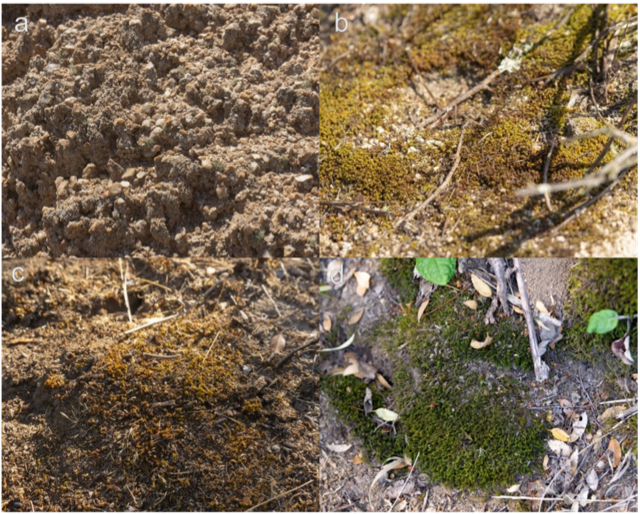
\includegraphics[width=1\textwidth]{img/M1-Figure_1.png}
	\caption{Sampled biological soil crust for PA (a), SG (b), LC (c), and NA (d).}
	\label{fig:M1-F1-Sampled_biocrust}
\end{figure}

\FloatBarrier

\begin{table}[h!]
\centering
\caption{Taxonomical composition of mosses and lichens in the biological soil crust for the study sites along the climatic gradient.}
\resizebox{\textwidth}{!}{%
\begin{tabular}{lllc}
\hline
\textbf{Site / Division} & \textbf{Family} & \textbf{Genus} & \textbf{No. species} \\
\hline
\textbf{PdA} & & & \\
Lichens & Cladoniaceae & \textit{Cladonia} sp. & 2 \\
        & Verrucariaceae & \textit{Placidium} sp. & 2 \\
        & Lecanoraceae & \textit{Lecidella} sp. & 1 \\
        & Rhizocarpaceae & \textit{Rhizocarpon} sp. & 1 \\
\hline
\textbf{SG} & & & \\
Mosses & Pottiaceae & \textit{Syntrichia} sp. & 2 \\
       & Pottiaceae & \textit{Tortella} sp. & 2 \\
Unidentified lichens & & & 2 \\
\hline
\textbf{LC} & & & \\
Mosses & Bartramiaceae & \textit{Philonotis} sp. & 1 \\
       & Bryaceae & \textit{Bryum} sp. & 1 \\
       & Pottiaceae & \textit{Syntrichia} sp. & 2 \\
       & Pottiaceae & \textit{Tortella} sp. & 2 \\
Unidentified mosses and lichens & & & 2 + 1 \\
\hline
\textbf{NA} & & & \\
Mosses & Amblystegiaceae & \textit{Acrocladium} sp. & 1 \\
       & Amblystegiaceae & \textit{Amblystegium} sp. & 1 \\
       & Bartramiaceae & \textit{Bartramia} sp. & 1 \\
       & Bryaceae & \textit{Bryum} sp. & 1 \\
       & Dicranaceae & \textit{Campylopus} sp. & 2 \\
       & Pterigynandraceae & \textit{Myurella} sp. & 1 \\
Unidentified liverworts, lichens, fungi & & & 2 + 2 + 1 \\
\hline
\end{tabular}}
\label{tab:taxonomical_composition}
\end{table}

\FloatBarrier

\subsection{Soil sampling and analyses}

For soil characterization, bulk topsoil samples (\SIrange[range-phrase=--,range-units=single]{0}{5}{\centi\meter}) were taken with metal-core sample augers directly under biocrust patches and in comparative zones without biocrust cover and sieved to \SI{2}{\milli\meter} after air drying. Bulk density (BD) and soil water content were determined gravimetrically. The particle size distribution was determined for seven fractions according to \citet{Kohn1929}, combining sieving of fractions $>$\SI{20}{\micro\meter} and pipetting of fractions $<$\SI{20}{\micro\meter}. Soil texture was interpreted according to the WRB soil classification system \citep{Jahn2006}. Soil pH was determined in water by a WTW pH 340 (WTW GmbH, Weilheim, Germany) using a Sentix 81 electrode, and electrical conductivity was measured with a conductivity meter (LE703, Mettler Toledo, USA). Total carbon (C\textsubscript{t}) and nitrogen (N\textsubscript{t}) of the bulk topsoil samples (\SIrange[range-phrase=--,range-units=single]{0}{5}{\centi\meter}) were analyzed using oxidative heat combustion at \SI{1150}{\degreeCelsius} in a Vario EL III elemental analyzer (Elementar Analysensysteme GmbH, Hanau, Germany). Total organic carbon (TOC) was corrected by the carbonate content of samples with pH $>$6.7. The carbonate content was determined from the volumetric titration of the reaction with 10\% HCl using a calcimeter (Eijkelkamp, Giesbeek, Netherlands).

The physical stability of soil aggregates was measured to quantify the destructive effect of water and mechanical forces through two-stage sieving: dry and wet \citep{Hartge2009}. Water-stable aggregates were measured by sieving \SI{200}{\gram} of undisturbed, air-dried soil samples, homogenized to \SI{30.0}{\milli\meter}, through a stack of sieves of decreasing mesh size (19.0, 14.7, 9.8, 6.8, 4.8, 3.3, \SI{2.0}{\milli\meter}, plus that collected the remainder below \SI{2.0}{\milli\meter}) and then repeating the same process underwater \citep{Six2000}. Finally, coarse fragments (stones) were removed, and the values for each size were calculated relative to the weight of the initial sample. With this aggregate stability data, accumulated frequency curves were calculated, and a set of stability indexes were estimated: difference in mean weight diameter of the aggregates ($\Delta$MWD) \citep{Hartge2009,Bavel1950,LoaizaPuerta2018}, difference in geometric mean diameter ($\Delta$GMD) \citep{Mazurak1950,Kemper1986}, water stability aggregate ratio (WSAR) \citep{Liu2014} and the proportion of soil macroaggregates of a diameter less than 2 mm (R<2 mm) \citep{Liang2015} as described below. $\Delta$MWD and $\Delta$GMD indicate how much the average diameter of soil aggregates changes between dry and wet conditions. The main difference between $\Delta$MWD and $\Delta$GMD is that the first considers a linear behavior between the different aggregate size classes, while the $\Delta$GMD considers a logarithmic fitting.

\subsubsection{Difference in mean weight diameter ($\Delta$MWD)}

    $$\Delta MWD = \frac{\sum_{i=1}^{n} X_i*W_i}{\sum_{i=1}^{n} W_i}$$
    where $W_i$ is the corrected mass proportion of stable aggregate fraction $i$ in the total \SIrange[range-phrase=--,range-units=single]{2}{30}{\milli\meter} aggregate fractions, and $X_i$ is the mean diameter of stable aggregate fraction $i$. and $n$ is the number of particle fractions.

\subsubsection{Difference in geometric mean diameter ($\Delta$GMD)}
    $$\Delta GMD = exp \left[\frac{\sum_{i=1}^{n} X_i\lg W_i}{\sum_{i=1}^{n} W_i}\right]$$
    where $X_i$ is the sieve opening size (mm), $W_i$ is the proportion of the total sample mass occurring in the $i$-size fraction, and $n$ is the number of particle fractions.

\subsubsection{Water stability aggregate ratio (WSAR)}

    $$WSAR = \frac{WSA}{A}*100$$
    where $WSA$ is the >2 mm water-stable aggregate content, and  $A$ is the >2 mm dry aggregate content.

\subsubsection{Proportion of soil macroaggregate of a diameter less than 2 mm (R$_{<2mm}$)}
    $$R_{<2mm}=\frac{W_{r>2}}{W_T}*100 = \left(1-\frac{W_{r<2}}{W_T}\right)$$
    where $W_{r>2}$ is the weight of macroaggregates with a diameter less than 2 mm, $W_T$ is the total sample weight, $W_{r<2}$ is the weight of microaggregates with a diameter less than 2 mm.
    
\subsection{Statistical analyses}

The influence of the climatic gradient (study site) and biocrust presence on physicochemical soil parameters and aggregate stability in 40 plots (4 study sites, 2 biocrust treatments, 5 replicates) were assessed by factorial generalized linear models (GLM) because of the lack of normal distribution for most of the variables according to the Shapiro-Wilk test. The link functions used for each model were selected based on the lowest Akaike information criterion (AIC) selection and characteristics of the data (skewness, counts, continuous variables, proportions) between Gaussian, Gamma, inverse Gaussian, and Tweedie distributions. Differences in treatments were tested using Tukey post-hoc-test with $p <0.05$ as significance criteria. The analyses were conducted in R 4.2.0 \citep{RCoreTeam2018}, and the GLM distributions were extended from the base R core with the Tweedie 2.3.3 package \citep{Dunn2017}. All visualizations were made with the package ggplot2 3.3.3 \citep{Wickam2016}.

\section{Results}
\subsection{Soil properties}

Soil pH was significantly affected by the climatic gradient (Figure \ref{fig:M1-F2-soil_properties_panel}), with mean values of 7.7 in PA, 6.2 in SG, 5.9 in LC, and 4.4 in NA, with acidification levels of 6.2 in BSC- to 5.9 in BSC+. In terms of electrical conductivity (EC), a remarkably higher value of \SI{2646.1}{\micro\siemens\per\centi\meter} in PA is outstanding in comparison with the low and homogeneous values of \SI{109.3}{\micro\siemens\per\centi\meter} for SG, \SI{153.8}{\micro\siemens\per\centi\meter} for LC, and \SI{102.3}{\micro\siemens\per\centi\meter} for NA. EC did not differ for the biocrust treatment. Nevertheless, when looking at the site and biocrust in combination, the BSC+ results in a reduction of the EC in PA; meanwhile, in SG, LC, and NA there was no noticeable change.

\begin{figure}[htbp] % Adjust placement specifiers [htbp] as needed
    \centering % Center the entire block of subfigures

    % --- Row 1 (3 figures) ---
    \begin{subfigure}[b]{0.32\textwidth} % Width suitable for 3 across
        \centering
        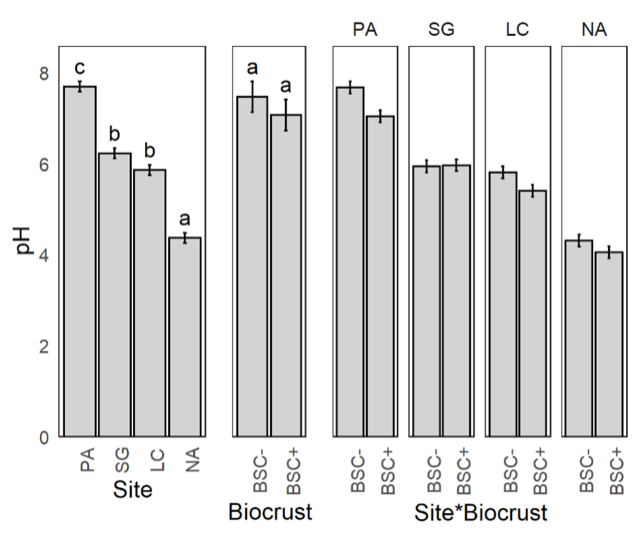
\includegraphics[width=\linewidth]{img/M1-Figure_2-01.png}
        % No caption or label needed here
    \end{subfigure}
    \hfill % Distribute space
    \begin{subfigure}[b]{0.32\textwidth}
        \centering
        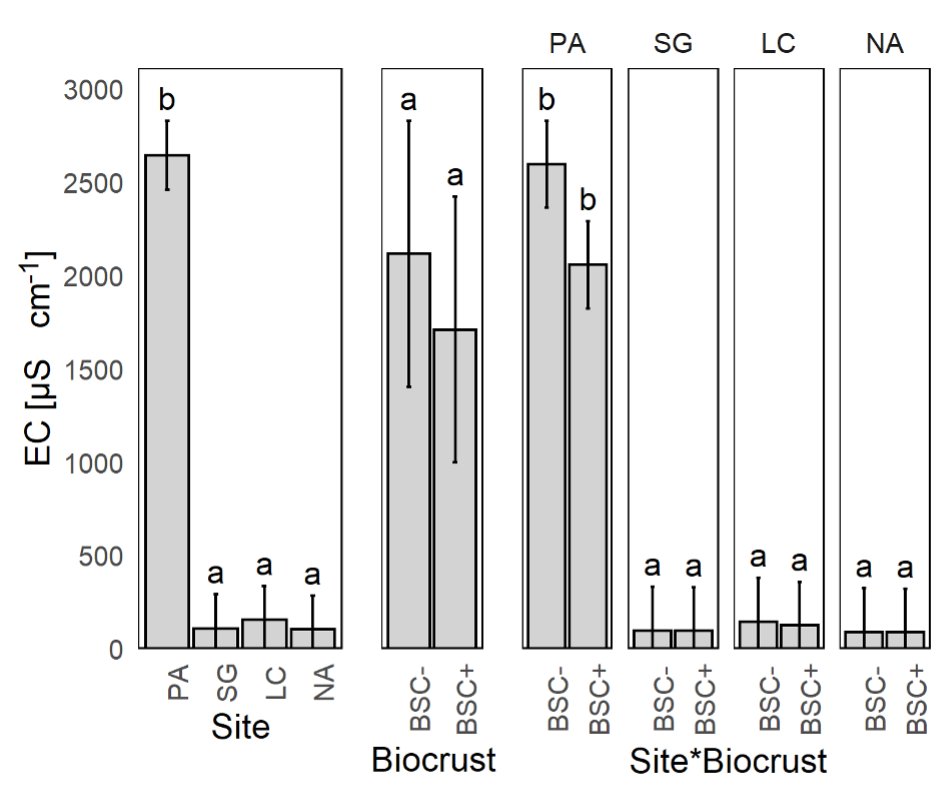
\includegraphics[width=\linewidth]{img/M1-Figure_2-02.png}
    \end{subfigure}
    \hfill
    \begin{subfigure}[b]{0.32\textwidth}
        \centering
        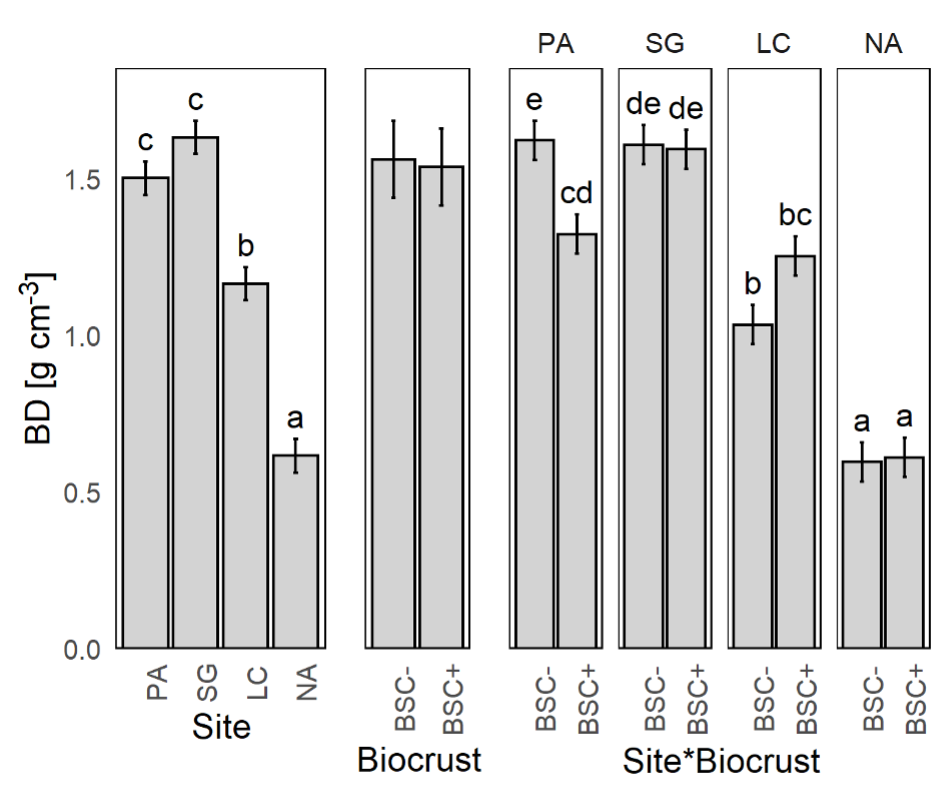
\includegraphics[width=\linewidth]{img/M1-Figure_2-03.png}
    \end{subfigure}

    \vspace{0.3cm} % Adjust vertical space between rows if needed

    % --- Row 2 (3 figures) ---
    \begin{subfigure}[b]{0.32\textwidth}
        \centering
        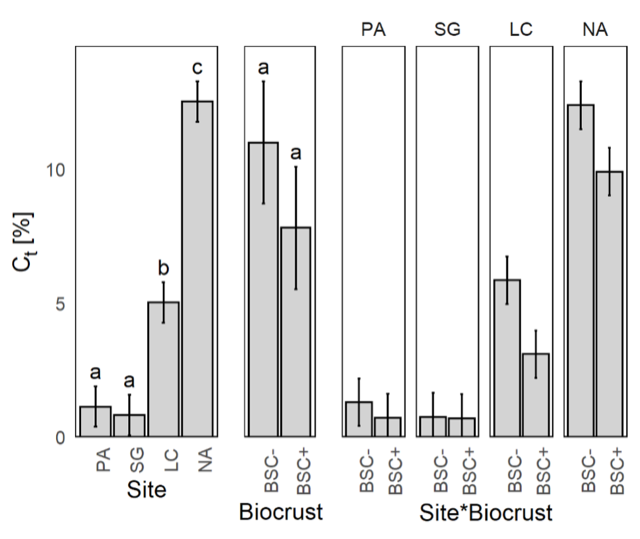
\includegraphics[width=\linewidth]{img/M1-Figure_2-04.png}
    \end{subfigure}
    \hfill
    \begin{subfigure}[b]{0.32\textwidth}
        \centering
        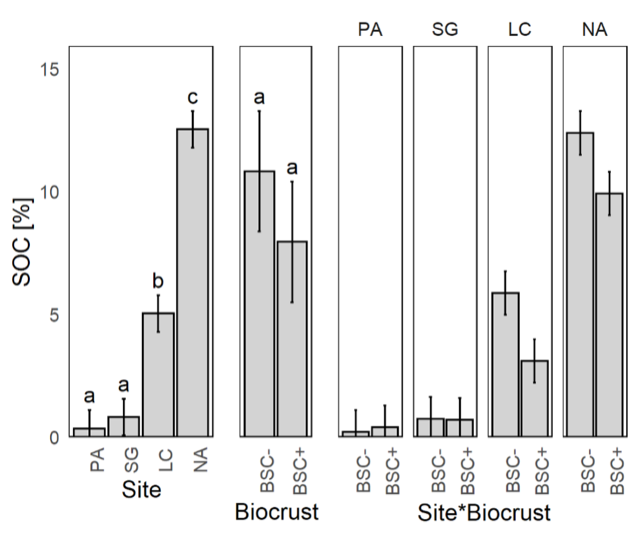
\includegraphics[width=\linewidth]{img/M1-Figure_2-05.png}
    \end{subfigure}
    \hfill
    \begin{subfigure}[b]{0.32\textwidth}
        \centering
        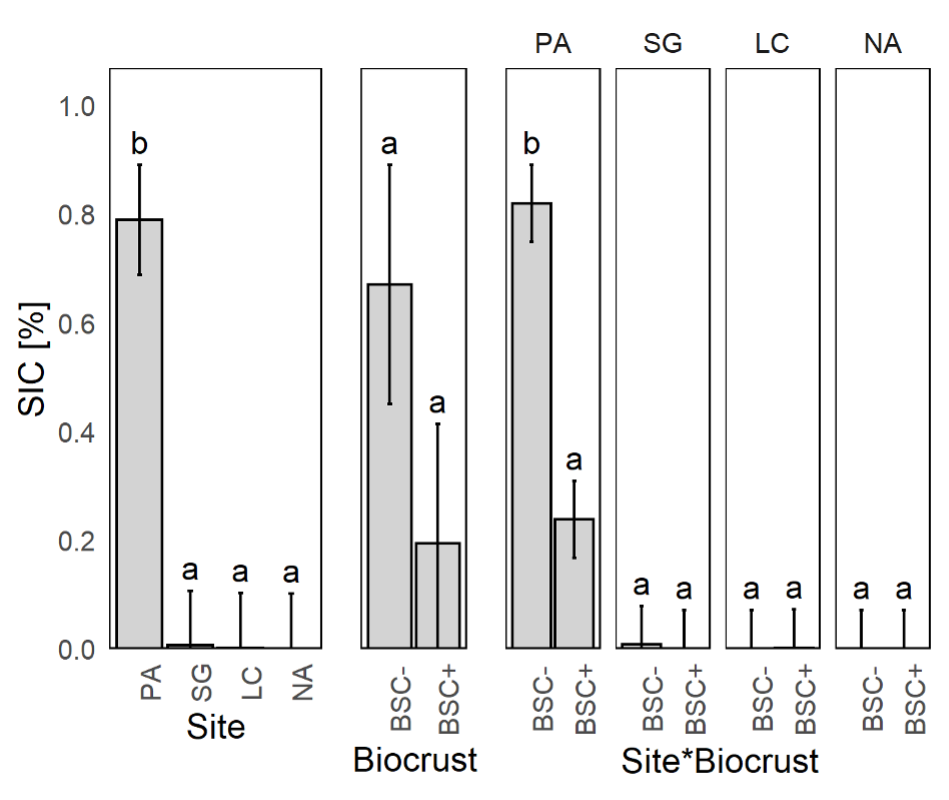
\includegraphics[width=\linewidth]{img/M1-Figure_2-06.png}
    \end{subfigure}

    \vspace{0.3cm}

    % --- Row 3 (3 figures) ---
    \begin{subfigure}[b]{0.32\textwidth}
        \centering
        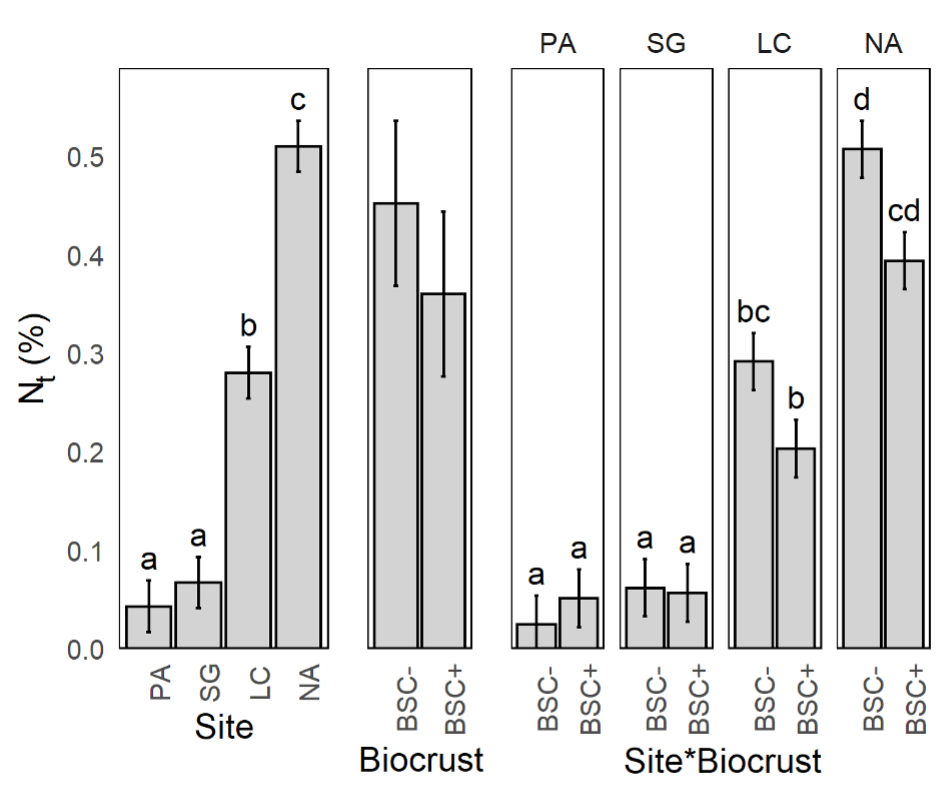
\includegraphics[width=\linewidth]{img/M1-Figure_2-07.png}
    \end{subfigure}
    \hfill
    \begin{subfigure}[b]{0.32\textwidth}
        \centering
        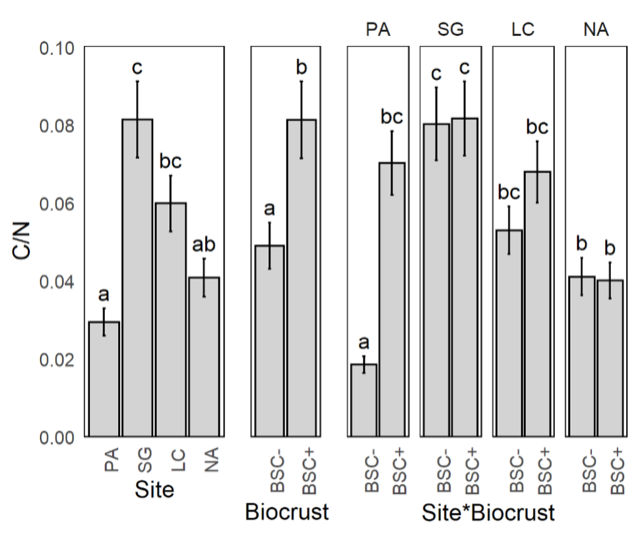
\includegraphics[width=\linewidth]{img/M1-Figure_2-08.png}
    \end{subfigure}
    \hfill
    \begin{subfigure}[b]{0.32\textwidth}
        \centering
        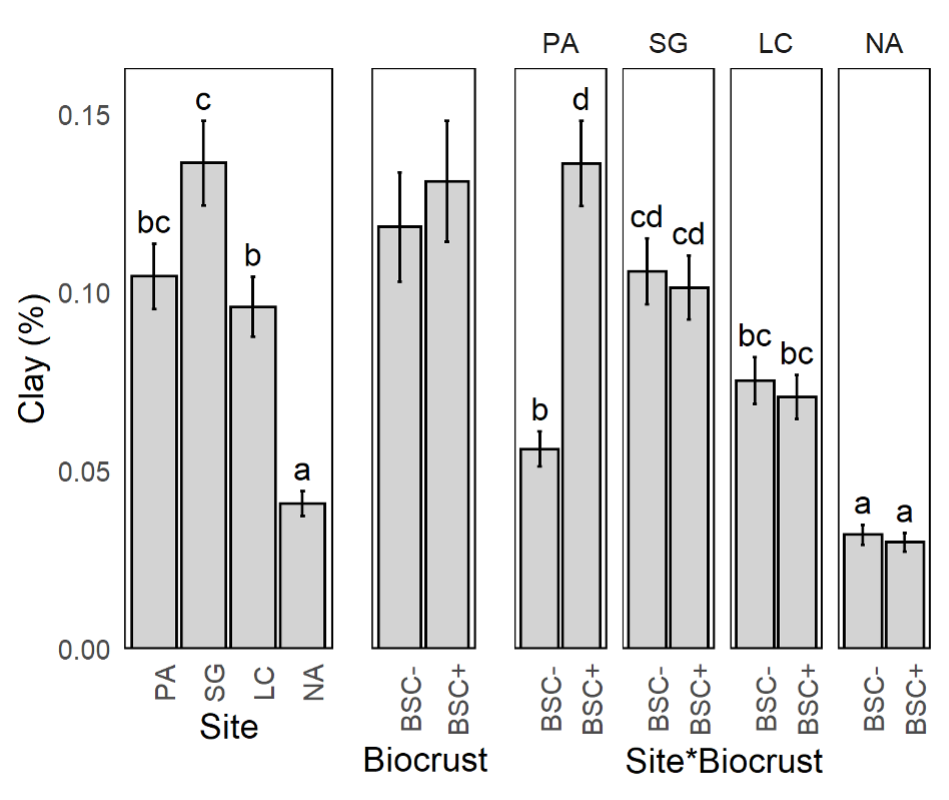
\includegraphics[width=\linewidth]{img/M1-Figure_2-09.png}
    \end{subfigure}

    \vspace{0.3cm}

    % --- Row 4 (2 figures, centered) ---
    % Use slightly wider subfigures here, pushed apart by \hfill
    \begin{subfigure}[b]{0.32\textwidth} % Width suitable for 2 across
        \centering
        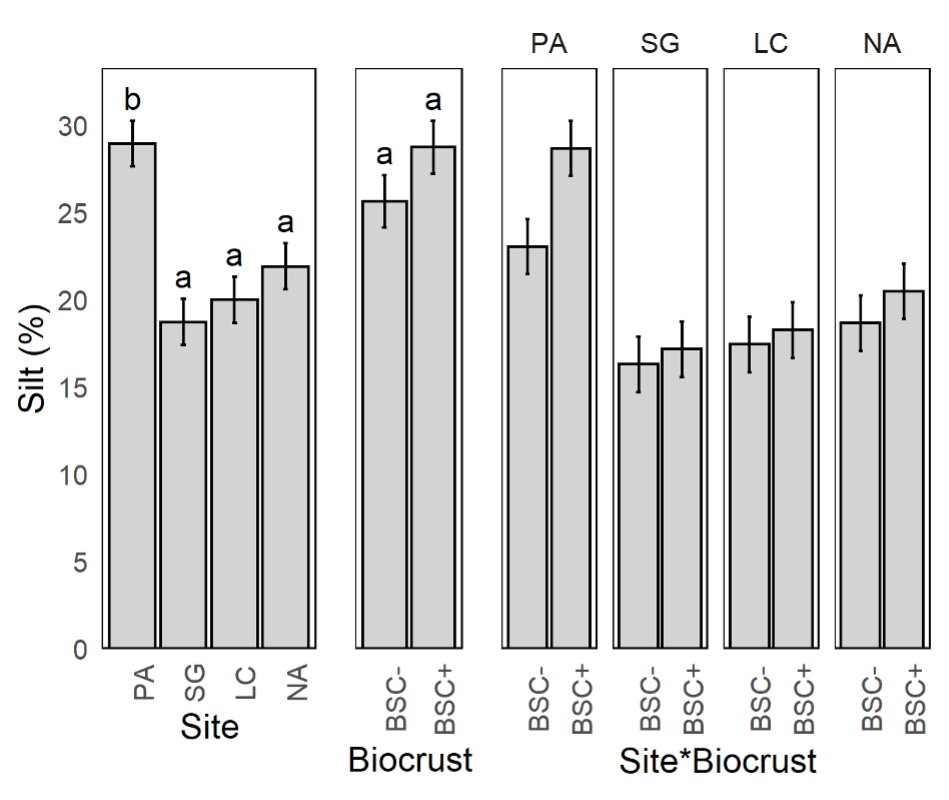
\includegraphics[width=\linewidth]{img/M1-Figure_2-10.png}
    \end{subfigure}
    \begin{subfigure}[b]{0.32\textwidth}
        \centering
        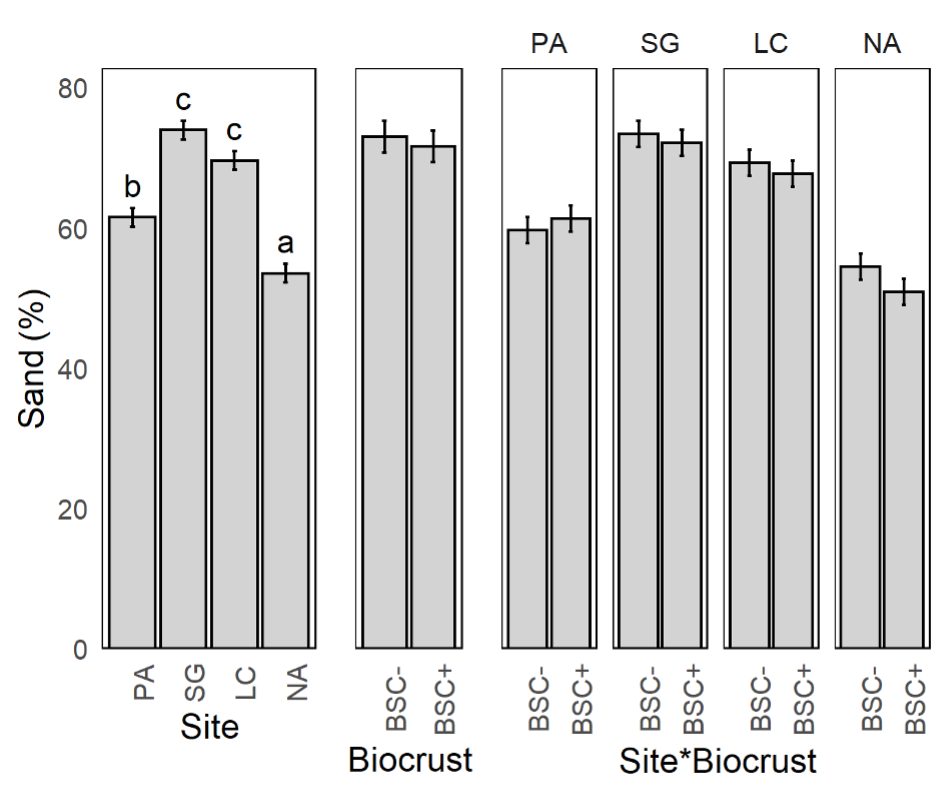
\includegraphics[width=\linewidth]{img/M1-Figure_2-11.png}
    \end{subfigure}

    % --- Main Caption and Label for the entire figure ---
    \caption{Mean and standard error of soil properties for Pan de Azúcar (PA), Santa Gracia (SG), La Campana (LC) and Nahuelbuta (NA), without (BSC-) and with biocrust cover (BSC+), and the interaction of both factors. (EC = electrical conductivity, BD = bulk density, C\textsubscript{t} = total carbon, SOC = soil organic carbon, SIC = soil inorganic carbon, N\textsubscript{t} = total nitrogen, C/N = carbon to nitrogen ratio). Significant factors include Tukey's Post-hoc-Test indicated by letters on the top of the bars. Different letters represent significant differences at $p <0.05$.}
    \label{fig:M1-F2-soil_properties_panel} % Use the same descriptive label

\end{figure}

Bulk density (BD) showed a significant difference between the study sites, with higher values in the two dryer sites, with \SI{1.5}{\gram\per\cubic\centi\meter} in PA, and \SI{1.6}{\gram\per\cubic\centi\meter} in SG, and a decrease in the more humid sites, with \SI{1.2}{\gram\per\cubic\centi\meter} in LC and \SI{0.6}{\gram\per\cubic\centi\meter} in NA. Biocrust showed no changes for BD in SG and NA, but in PA BSC+ resulted in a reduction of the BD of 18.2\%, while in LC BSC+ showed an increase in BD of 21.9\% (Figure \ref{fig:soil_properties_panel}).

Total carbon (C\textsubscript{t}) content was directly proportional to the humidity along the climatic gradient (Figure \ref{fig:soil_properties_panel}), with values of 1.1\% in PA, 0.8\% in SG, 5.0\% in LC, and 12.5\% in NA, but with a significant decrease when the BSC+ is present, from 5.6\% to 4.2\% in average. Soil inorganic carbon (SIC) was significantly higher in PA, with an average of 0.8\% of the mass of the soil, while in SG, LC, and NA, it was not found. When looking at the SIC along the different sites and under biocrust in combination, the BSC+ results in a reduction of 70.1\% in the SIC for PA, while in SG, LC and NA was no change. Soil organic carbon (SOC) showed a similar pattern as C\textsubscript{t}, with a reduction in PA to 0.3\% and the same 0.8\% in SG, 5.0\% in LC, and 12.5\%. Total nitrogen (N\textsubscript{t}) content was directly proportional to the humidity along the climatic gradient, with values of 0.04\% for PA, 0.07\% for SG, 0.28\% for LC and 0.51\% for (Figure \ref{fig:soil_properties_panel}). BSC+ showed a reduction of 30.3\% in LC and 22.3\% in NA, while the N\textsubscript{t} content remained stable in PA and SG under the influence of BSC. The relation between C\textsubscript{t} and N\textsubscript{t}, expressed as C/N, showed significantly different values of 33.9 in PA, 12.3 in SG, 16.7 in LC, and 24.5 in NA on average; and with a significant decrease from 27.0 in BSC- to 16.7 in BSC+ (Figure \ref{fig:soil_properties_panel}). It is important to note that although PA and NA present the highest values, the condition changes diametrically when observed together with the BSC+ treatment, with a large dispersion in PA and stable values in NA.

The distribution of the soil particle size classes did not show clear patterns along the climatic gradient, with PA deviating from it in all cases. Despite this, the observed values were significant, with clay values of 9.6\% for PA, 7.3\% in SG, 10.4\% in LC, and 24.6\% in NA, while when looking at the interaction between site and biocrust, there is an increase of 143.4\% in clay content for the BSC+ condition, while for SG, LC and NA was no difference; silt with 28.9\% in PA, 18.7\% in SG, 20.0\% in LC and 21.9\% in NA; and sand with 61.5\% in PA, 73.9\% in SG, 69.6\% in LC and 53.5\% in NA. When biocrusts were present, a significant decrease from 13.6\% to 12.6\% in clays and an increase from 21.2\% to 23.6\% in silt was observed, with higher dispersion for the arid site (PA) (Figure \ref{fig:soil_properties_panel}).

\subsection{Soil aggregate stability}

Dry sieving showed a significant difference between study sites but not for the biocrust treatment (Figure \ref{fig:M1-F3}). Dry aggregates in the \SIrange[range-phrase=--,range-units=single]{19.5}{30.0}{\milli\meter} range showed significantly different values of 4.4\% in PA, 1.2\% in SG, 5.5\% in LC, and 36.2\% in NA. The fraction \SIrange[range-phrase=--,range-units=single]{9.5}{19.0}{\milli\meter} revealed differences in the interaction between study sites and biocrusts, increasing the proportion of aggregates from 13.2\% in PA to 19.3\% SG and 29.3\% in LC, not in NA with only 2.9\% in the presence of biocrusts. The aggregates between \SIrange[range-phrase=--,range-units=single]{6.7}{9.5}{\milli\meter} showed a significant decrease from 13.3\% in PA, 5.2\% in SG, 6.5\% in LC, and 4.1\% in NA. In interaction with biocrusts, it showed a significant increase in the proportion when it was present. The fraction from \SIrange[range-phrase=--,range-units=single]{4.7}{6.7}{\milli\meter} showed significantly different values of 13.6\% in PA, 3.4\% in SG, 5.0\% in LC, and 5.6\% in NA, while the interaction with biocrusts showed a significant increase when is present (BSC+). Aggregates from \SIrange[range-phrase=--,range-units=single]{3.4}{4.7}{\milli\meter} size showed significance among study sites, with 9.8\% in PA, 3.6\% in SG, 4.4\% in LC, and 7.9\% in NA. Aggregates between \SIrange[range-phrase=--,range-units=single]{2.0}{3.4}{\milli\meter} showed a slightly similar amount of 9.9\% in PA, 5.9\% in LC, and 14.3\% in NA, but with a minor proportion of 4.9\% in LC, while when biocrust is present in LC, it showed a slight decrease. Finally, for the dry sieved aggregates under \SI{2}{\milli\meter}, there was a significant reduction for the study sites, with values of 69.1\% in SG and 47.3\% in LC relative to 30.1\% in PA, but not in NA with 28.9\%; while the biocrust effect in interaction with the site is significant with 60.6\% in SG and 40.8\% in LC, indicating the same proportion of aggregates in this site for SG with 30.0\% and NA with 39.8\%.

In a second stage, aggregate stability under wet conditions was characterized, with a clear difference between sites, while biocrusts had a significant effect only on the aggregate size classes $<$\SI{2.0}{\milli\meter} and \SIrange[range-phrase=--,range-units=single]{19.0}{30.0}{\milli\meter} (Figure \ref{fig:M1-F3}). At the same time, the fraction \SIrange[range-phrase=--,range-units=single]{19.0}{30.0}{\milli\meter} showed an increasing significant pattern in the amount of aggregates, with 2.8\% in NA, 0.8\% in SG, 8.9\% in LC, and 29.9\% in NA, while biocrusts significantly increased the proportion of aggregates by 35.6\%, from 9.0\% for BSC- to 12.2\% for BSC+. For the fraction \SIrange[range-phrase=--,range-units=single]{9.5}{19.0}{\milli\meter}, there were significant differences between the study sites, the biocrust effect, and its interactions, with an increase from 5.4\% to 11.7\% on average when biocrusts were present. The wet sieved aggregates in the range of \SIrange[range-phrase=--,range-units=single]{6.7}{9.5}{\milli\meter} showed significant differences only between the study sites, with 10.6\% in PA, 2.5\% in SG, 4.2\% in LC and 4.3\% in NA. Wet aggregates in the range of \SIrange[range-phrase=--,range-units=single]{4.7}{6.7}{\milli\meter} showed significant differences between the study sites with 10.6\% in PA, 2.3\% in SG, 3.7\% in LC and 5.8 in NA. The fraction between \SIrange[range-phrase=--,range-units=single]{3.4}{4.7}{\milli\meter} showed only significant differences between the study sites, with 6.9\% in PA, 2.2\% in SG, 3.0\% in LC, and 6.1\% in NA. Aggregates ranging from \SIrange[range-phrase=--,range-units=single]{2.0}{3.4}{\milli\meter} showed differences between the study sites, with 5.8\% in PA, 3.2\% in SG, 4.2\% in LC, and 6.8\% in NA. The fractions under \SI{2.0}{\milli\meter} were significantly different for the study sites, with 58.3\% in PA, 79.6\% in SG, 62.4\% in LC, and 41.3\% in NA; and for biocrusts from 63.9\% for BSC+ treatment to 56.9\% for BSC- treatment.

\begin{figure}[H]
	\centering
	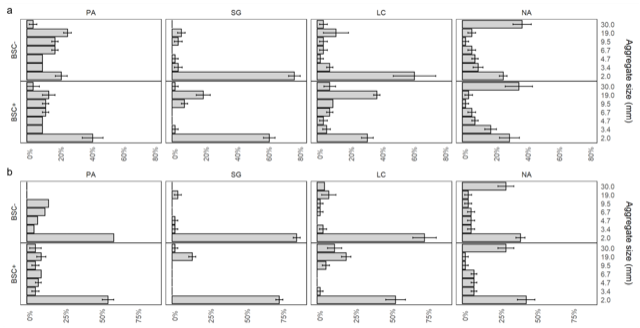
\includegraphics[width=1\textwidth]{img/M1-Figure_3.png}
	\caption{Mean value and standard error of aggregate proportion for dry (a) and wet (b) sieved fractions for Pan de Azúcar (PA), Santa Gracia (SG), La Campana (LC), and Nahuelbuta (NA) for biocrust (BSC+) and non-biocrust (BSC-) treatments. Significant factors and corresponding models for response variables are included in Appendix \ref{tab:appendix_a}.}
	\label{fig:M1-F3}
\end{figure}


When comparing the changes of the aggregate distributions between wet and dry conditions (Figure \ref{fig:M1-F4}), an irregular pattern was observed, with a general decrease in most of the analyzed fractions, except for an increase in the amount of aggregates of \SI{19.0}{\milli\meter} for NA. This was even higher than for the BSC+ treatment. It is important to mention that NA also showed a slight increase in the proportion of \SI{9.5}{\milli\meter} and \SI{6.7}{\milli\meter} aggregates.

\begin{figure}[H]
	\centering
	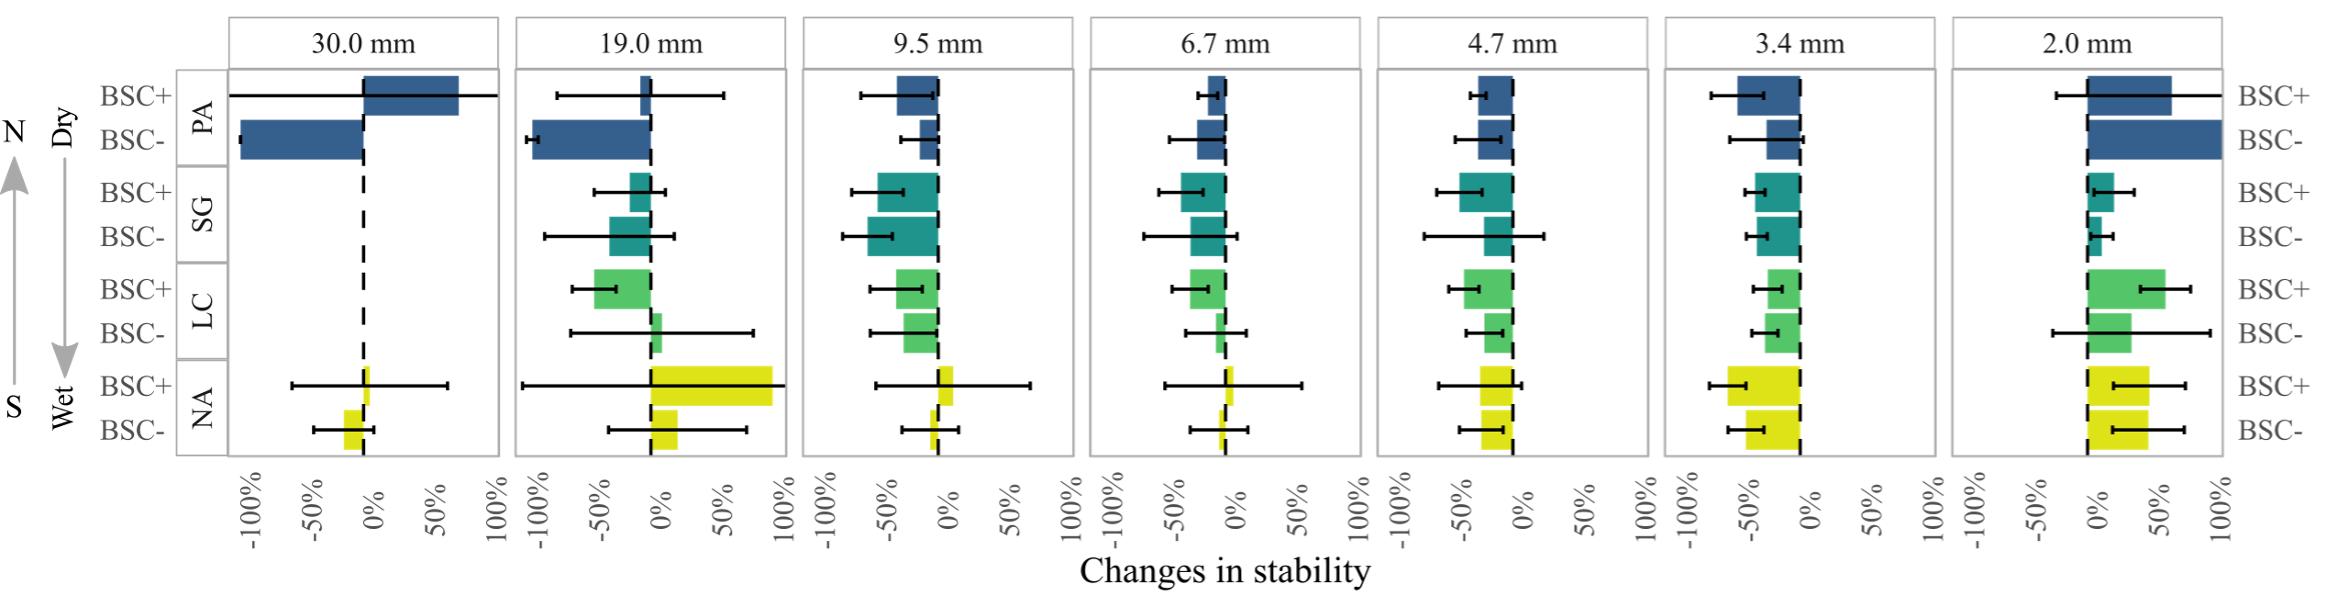
\includegraphics[width=1\textwidth]{img/M1-Figure_4.png}
	\caption{Mean and standard deviation of aggregate size distribution changes between dry and wet sieving for the sites Pan de Azúcar (PA), Santa Gracia (SG), La Campana (LC), and Nahuelbuta (NA) for biocrust (BSC+) and non-biocrust (BSC-) treatments. Error bars were, in some cases, truncated for better visualization.}
	\label{fig:M1-F4}
\end{figure}

Soil aggregate stability was evaluated through different indexes to integrate the different sizes and sieving conditions in a summary value. The difference in mean weight diameter of the aggregates ($\Delta$MWD) showed no significance in any of the conditions (Figure \ref{fig:M1-F5}). However, there was a significant difference in the difference of the geometric mean diameter of the aggregates ($\Delta$GMD) for the study sites, with values of \SI{1.86}{\milli\meter} for PA, \SI{1.2}{\milli\meter} for SG, \SI{1.4}{\milli\meter} for LC, in comparison with the more stable condition of \SI{0.83}{\milli\meter} for NA. The water-stable aggregates ratio was significant for the study sites, showing differences between NA with 81.1\% and the other study sites (57.7\% PA, 66.2\% SG, and 73.4\% LC). The ratio of soil macroaggregates of a diameter less than \SI{2.0}{\milli\meter} (R\textsubscript{$<$\SI{1.4}{\milli\meter}}) presents differences in the study sites and for biocrust treatments. SG showed a value of R\textsubscript{<\SI{2}{\milli\meter}} of 79.6\% and NA of 41.9\%, which was different from PA and LC, with 58.6\% and 62.4\%, respectively. For biocrust treatments, R\textsubscript{$<$\SI{1.4}{\milli\meter}} changed from 63.7\% to 57.5\% with biocrusts, indicating a biocrust-induced decrease in the proportion for this fraction. Finally, according to the analyzed indexes, NA showed the most stable conditions, and alternating PA and SG showed the most unstable conditions.

\begin{figure}[H]
	\centering
	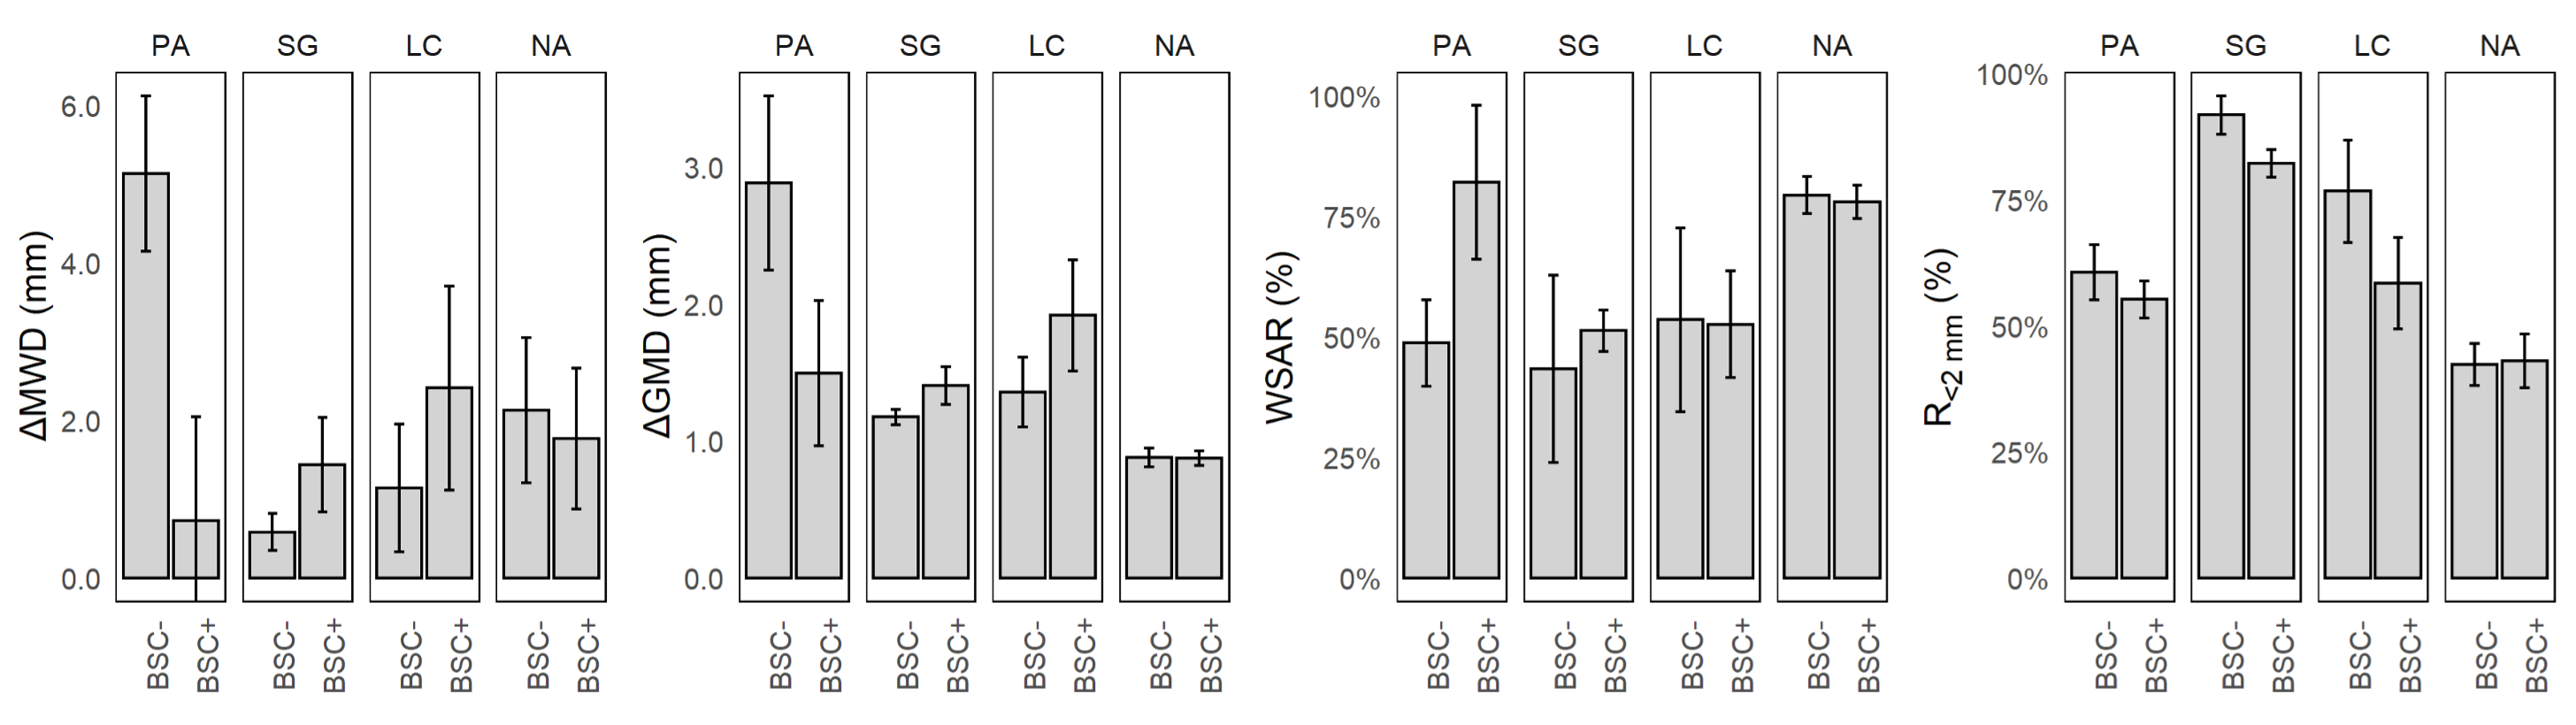
\includegraphics[width=1\textwidth]{img/M1-Figure_5.png}
	\caption{Mean and standard error of aggregate stability indexes for Pan de Azúcar (PA), Santa Gracia (SG), La Campana (LC),
    and Nahuelbuta (NA) for biocrust (BSC+) and non-biocrust (BSC-) treatments. $\Delta$MWD=difference in mean weight diameter,
    $\Delta$GMD=difference in geometric mean diameter, WSAR=water stability aggregate ratio, R\textsubscript{<\SI{2}{\milli\meter}}=ratio of aggregates less than \SI{2}{\milli\meter}. Significant factors and corresponding models for response variables are included in Appendix \ref{tab:appendix_a}.}
	\label{fig:M1-F5}
\end{figure}

As shown in Figure \ref{fig:M1-F2-soil_properties_panel}, the climatic gradient (site) had significant pH, electrical conductivity (EC), bulk density (BD), total carbon (C\textsubscript{t}), soil organic carbon (SOC), soil inorganic carbon (SIC), total nitrogen (N\textsubscript{t}), C/N, clay, silt, sand, dry and wet aggregates under \SI{30}{\milli\meter}, $\Delta$GMD, WSAR, R\textsubscript{<\SI{2}{\milli\meter}}. Biocrust treatments were significant for clay, silt, pH, EC, C\textsubscript{t}, SOC, SIC, N\textsubscript{t}, C/N, and wet aggregates from \SIrange{9.5}{30.0}{\milli\meter} and $>$\SI{2}{\milli\meter}, and R\textsubscript{<\SI{2}{\milli\meter}}. Finally, the interaction of the site and biocrusts was significant for clay, bulk density (BD), total nitrogen (N\textsubscript{t}), dry aggregates from \SIrange{4.7}{19.0}{\milli\meter} and \SIrange{0}{3.4}{\milli\meter}, wet aggregates from \SIrange{9.5}{30.0}{\milli\meter}, and $\Delta$MWD.

\section{Discussion}

\subsection{Aggregate stability and soil properties along the climatic gradient}

The climatic gradient has a significant effect on the stability of soil aggregates. Using the geometric mean diameter ($\Delta$GMD), an index that replaces the linear fitting of $\Delta$MWD with a logarithmic one, significant differences for the study sites along the climatic gradient can be observed ($p-value: <0.001$). When soil aggregate stability was evaluated with the difference in mean weight diameter ($\Delta$MWD), it did not show significant changes along the climatic gradient. WSAR, an index that shows the ratio of aggregates that persist stably after disruption by water, showed a similar behavior as $\Delta$MWD. The main difference between $\Delta$MWD and $\Delta$GMD is that $\Delta$GMD performs better in non-uniform particulate substances \citep{Hatch1929,Gardner1956}, which corresponds to soils equilibrated in the content of sand, silt, and clay \citep{Mazurak1950} and pointing soil texture indirectly as a critical factor in aggregate stability along the climatic gradient. Further, considering the $\Delta$GMD data, an increase in stability was observed as moving along the climatic gradient to higher water availability conditions except for SG. The lower value of $\Delta$GMD for SG indicates comparably higher aggregate stability as it would be expected when we assume a steady trend from arid to humid climate. In PA, in the drier north, the condition proved to be less stable than NA, despite the high content of inorganic carbon. SG presented the highest ratio of unstable aggregates under the studied range of sizes (highest R\textsubscript{<\SI{2}{\milli\meter}}) and NA the lowest, with close to half of it, indicating augmented aggregate stability in the complementary range of sizes.

The effect of the climatic gradient is not only expressed in the stability of soil aggregates, but it is also present with different intensities in a variety of soil properties. The pH decreases continuously from the northern arid to the southern humid study site in accordance with \citet{Bernhard2018}. The high pH in PA can be attributed to the constant input of atmospheric aerosols, e.g., salts, gypsum, and calcium carbonates \citep{Ewing2006} in combination with the arid climate that allows salts to accumulate in the topsoil \citep{Slessarev2016}. Whereas in the southern sites, the forwarding increase of precipitations results in a reduction in the pH due to leaching of soluble salts \citep{Slessarev2016} and an increase in soil respiration \citep{Orchard1983}. The accumulation of soluble salts is well established for the arid site PA, as saline conditions \citep{Allison1954} are indicated by the high electrical conductivity value. These higher amounts of salts have a strong effect in structure degradation dynamics, linked to the destabilizing effect of sodium and stabilizing of carbonates \citep{Corwin2021}. Although C\textsubscript{t} and N\textsubscript{t} follow the climatic gradient, when comparing the C/N, PA and NA have higher values. High values of the C/N indicate a nitrogen limitation of plants and other organisms \citep{Brust2019}, pointing out that this occurs at the two opposite sites along the climatic gradient. This could be explained by the biological activity \citep{Zhang2013}, which may be close to a physiological limitation in the case of NA, while for PA, it may indeed be due to low nitrogen availability \citep{Hooper1999}. However, there was also a high amount of carbonates in PA, which makes PA hardly comparable in terms of C\textsubscript{t}. Despite the properties following the climatic gradient, SG deviates from the other sites in terms of higher bulk density (BD), lower clay, and higher sand content. This can indicate a degraded condition for the semi-arid site caused by the current land use, including grazing \citep{Armesto2007}, compacting the surface and thus activating erosive processes \citep{Scholten2019}, in favor of the accumulation of sand particles \citep{Govers1985}. The aggregate distribution stresses this finding, where SG has a lower proportion of water-stable aggregates $>$\SI{2}{\milli\meter} and a higher water-destabilization of aggregates between \SIrange{9.5}{4.7}{\milli\meter}, indicating that the nature of the structuring agent in that zone is water-soluble.


\subsection{Biocrusts altering soil properties along the climatic gradientt}

Despite these factors beyond the climatic gradient, biocrusts showed effects on clay, silt, pH, C\textsubscript{t}, N\textsubscript{t}, C/N, and wet aggregates from \SIrange{9.5}{30.0}{\milli\meter} and $>$\SI{2}{\milli\meter}. However, as this was an observational study, it only allows establishing associations between factors and not cause-effect relationships \citep{Cox1992,Rosenbaum2005}. It is thus possible that changes in soil characteristics promote the biocrust establishment, as well as that biocrust establishment triggers changes in these properties \citep{Belnap2003}.

The biocrust treatments showed a significant decrease in pH ($p-value: 0.002404$), reflecting the biological activity of its constituent organisms, which acidifies the soil due to the carbon dioxide released by cellular respiration \citep{Bachar2010}. The pH values reported by \citet{Bernhard2018} are in the same range as ours but without differentiating between BSC+ and BSC-, as this factor was not part of their study. The content of C\textsubscript{t} and N\textsubscript{t} were significantly different when biocrusts were present, but it did not affect any aggregate sizes or stability indexes. In this sense, biocrusts play a role in the carbon and nitrogen cycles \citep{Chen2000}, as they are formed mainly by photosynthetic and nitrogen-fixing organisms (Maestre et al., 2013), but it has not had an immediate impact on the soil aggregate stability and points out that the primary stabilizing agent is of organic origin \citep{Wagner2007,Six2004}.

Considering the stabilizing effect of biocrusts on wet sieved aggregates between 9.5 and \SI{30}{\milli\meter}, we could show that it occurs prominently at the three northern sites, whereas in NA there was no difference with and without biocrusts. This points to a threshold in the biocrust-induced stabilization of the soil aggregates between LC and NA and partially confirms our initial assumption that biocrusts have the greatest effect in arid conditions. However, the effect on aggregate stability for the wet condition varies according to the variable used, being specific for limited aggregate sizes in terms of mechanical disturbances (dry sieving) but without a substantial improvement concerning water stability (wet sieving). This lack of difference in wet sieved aggregate point to a non-soluble nature of the stabilizing agents, which can be attributed to stabilization due to organic structures and exudates \citep{Rillig2004}, and stress the idea that NA differs to the other sites in the mechanisms of aggregate stabilization as a local adaptation, where due to the higher proportion of precipitation, is conducted by water stable mechanisms.

Soil aggregate stability showed clear differences along the climatic gradient. However, when considering the effect of biocrusts, differences were limited to the smallest aggregate size class (R\textsubscript{$<$\SI{1.4}{\milli\meter}) referring to changes in microaggregates size distribution as described by \citet{Totsche2018}. Further, a difference for wet sieved aggregates with and without biocrusts between 9.5 and \SI{30.0}{\milli\meter} point to biocrust-induced stabilization of soil aggregates.

The results indicate that soil aggregate stabilization mechanisms are different in PA than at the other sites. With that in mind, it was found that in PA, biocrusts grow in areas with a lower content of clay and higher content of silt, which implies increased nutrient availability and water-holding capacity \citep{Chen2020}, while the sand fraction was not related. However, the method used can amplify that difference since the determination of particle size distribution does not consider coarse fragments \citep{Kohn1929}, which were abundant at PA. In addition, the soil covered with biocrusts showed a lower value for bulk density (BD) only for PA, while in the other sites, this property was not affected. This can be interpreted as a biocrust-induced decrease in soil density due to increased intra- and extra-aggregate porosity and organic matter \citep{Whitney2017} or that biocrusts grow under the least limiting condition \citep{Bowker2014}. Soils with biocrust cover showed a trend of lower electrical conductivity, which can be explained by the inhibition of biocrusts by toxicity due to the accumulation of salts in the soil, or to the consumption of salts as a source of nutrients by the organisms in the biocrusts \citep{Abed2019}.

Biocrust plays a role along the climatic gradient affecting different properties, i.e., clay, silt, pH, C\textsubscript{t}, N\textsubscript{t}, C/N, and wet aggregates from \SIrange[range-units=single]{9.5}{30.0}{\milli\meter} and $>$\SI{2}{\milli\meter}. Nevertheless, the way that each property change responds to local conditions: In the arid northernmost site, there is a strong influence of the salts in terms of stabilization and establishment of biocrusts, while at the southernmost site, there is no stabilization of the aggregates, but a contribution to the carbon and nitrogen contents. The most consistent property along the climatic gradient was pH, an indicator of biological activity. However, at the scale of the climatic gradient it is not possible to distinguish the origin of biological activity between plants, microorganisms, fungi, bacteria, etc. Finally, considering the largest size of the persistent wet aggregates match the characteristics attributed to fungi and bryophytes, capable of retaining micro-aggregates and soil particles between their hyphae and rhizoids, respectively \citep{Kleber2007,Six2004,Totsche2018} and points to this as the most significant mechanism of soil aggregate stabilization of biocrusts.

\section{Conclusions}

This study aimed to investigate how and to what extent biocrusts stabilize soil aggregates along an arid to humid climatic gradient in Chile. We show that biocrusts play a role in soil aggregate stability along the climatic gradient by increasing the stability for wet aggregates from \SIrange[range-units=single]{9.5}{30.0}{\milli\meter} and $>$\SI{2}{\milli\meter}. Bicorusts also modify other soil properties such as C\textsubscript{t}, N\textsubscript{t}, C/N, clay, and sand, indicating an initial accumulation of organic matter that then give place to aggregation processes. The biocrusts effect on aggregates stability was lower under humid climate conditions, which indicates a transition in the main biotic agents driving the aggregation of the soil surface, moving from biocrust communities in arid regions to vascular plants in humid conditions.
Finally, we conclude that the biocrusts in our study area showed to be a valuable agent in stabilizing the upper topsoil layer, but for a narrow spectrum of conditions and mostly under arid conditions. Therefore, the effect could be considered a transition in ecological succession toward a stable ecosystem. In this process, biocrusts improve conditions for other more demanding species, such as vascular plants, initially improving the availability of carbon and nitrogen in the soil.

\section*{Appendices}

\begin{table}[htbp] % [htbp] placement specifier (Here, Top, Bottom, Page)
\centering % Center the table on the page
\caption{Appendix A. Significant factors for response variables based on generalized linear models. Models with significant interaction also include the predictors as simple parameters based on marginality principle. \\ % Line break in caption
\textit{(p-value $\le$ 0: "***"; p-value $\le$ 0.001: "**"; p-value $\le$ 0.01: "*")}} % Significance key (using <= for clarity)
\label{tab:appendix_a} % Label for cross-referencing
\begin{tabular}{@{}lllll@{}} % Left-aligned columns, @{} removes extra space at edges
\toprule
Dependent variable & Distribution & \multicolumn{3}{c}{Significance for independent variable} \\
\cmidrule(lr){3-5} % Rule under the multicolumn header only (trimmed left and right)
 & (link-function for GLM) & Site & Biocrust & Site $\times$ Biocrust \\ % Use $\times$ for multiplication
\midrule
Clay	& Gaussian	& ***	& *	& \\
Silt	& Inverse Gaussian	& ***	& *	& \\
Sand	& Gaussian	& ***	& 	& \\
Fine Silt	& Tweedie	& ***	& 	& * \\
Medium silt	& Tweedie	& ***	& ***	& * \\
Coarse silt	& Tweedie	& ***	& 	&  \\
Very fine sand	& Gaussian	& ***	& 	&  \\
Fine sand	& Tweedie	& ***	& 	&  \\
Medium sand	& Gaussian	& ***	& 	&  \\
Coarse sand	& Tweedie	& ***	& 	&  \\
pH	& Gaussian	& ***	& **	&  \\
EC	& Tweedie	& ***	& 	&  \\
BD	& Gaussian	& ***	& 	& ** \\
N\textsubscript{t}	& Gamma	& ***	& 	& ** \\ % For Nt subscript
C\textsubscript{t}	& Tweedie	& ***	& **	&  \\ % For Ct subscript
C/N	& Tweedie	& ***	& **	&  \\
19.0-30.0 mm Dry	& Tweedie	& ***	& 	&  \\
9.5-19.0 mm Dry	& Tweedie	& ***	& 	& ** \\
6.7-9.5 mm Dry	& Tweedie	& ***	& 	& ** \\
4.7-6.7 mm Dry	& Tweedie	& ***	& 	& * \\
3.4-4.7 mm Dry	& Tweedie	& ***	& 	&  \\
2.0-3.4 mm Dry	& Tweedie	& ***	& 	& * \\
\textless2.0 mm Dry	& Tweedie	& ***	& 	& *** \\ % Use \textless for less than symbol
19.0-30.0 mm Wet	& Tweedie	& ***	& *	& ** \\
9.5-19.0 mm Wet	& Tweedie	& *	& **	& * \\
6.7-9.5 mm Wet	& Tweedie	& ***	& 	&  \\
4.7-6.7 mm Wet	& Tweedie	& ***	& 	&  \\
3.4-4.7 mm Wet	& Tweedie	& ***	& 	&  \\
2.0-3.4 mm Wet	& Tweedie	& ***	& 	&  \\
\textless2.0 mm Wet	& Tweedie	& ***	& *	&  \\ % Use \textless for less than symbol
$\Delta$MWD	& Gaussian	& 	& 	&  \\ % Use \Delta for Greek Delta
$\Delta$GMD	& Tweedie	& ***	& 	&  \\ % Use \Delta for Greek Delta
WSAR	& Gaussian	& 	& 	&  \\
R\textless2 mm	& Gaussian	& ***	& *	&  \\ % Use \textless for less than symbol
\bottomrule
\end{tabular}
\end{table}

\FloatBarrier

\section*{Data availability}

The data that support the findings of this study are available from the corresponding author upon request.

\section*{Code availability}

The code that supports the findings of this study are available from the corresponding author upon request.

\section*{Author contribution}

TS, DW, CWM, OS, and StS conceptualized the study. OS, KW, and NRM collected the soil samples. StS collected and analyzed the biocrust samples, and NRM analyzed the soil samples. NRM performed the analyses and prepared the manuscript.

\section*{Competing interests}


The authors declare that they have no conflict of interest.

\section*{Acknowledgments}

We are deeply grateful to the students, technical assistants, and colleagues who helped in the field and laboratory phases. A special thanks to Martin Nebel and Sonja Thielen for their help in classifying bryophytes and lichens. Oliver Burkhardt (GFZ German Research Centre for Geosciences) and Franziska Steiner (Technical University of Munich) for their support in the field. Hugo Pérez for his help and experience in the soil physics laboratory of the Universidad de Chile. We are grateful to the Chilean National Forest Corporation (CONAF) and Sucesión Gálvez Muñoz, who provided access to the study sites. The study was funded by the German Science Foundation DFGSPP 1803 (EarthShape; www.earthshape.net). We acknowledge support by Open Access Publishing Fund of University of Tübingen.


\chapter{Biocrusts as climate-dependent regulators of erosion, water and nutrient cycling}
\label{chap:manuscript2} % Label for potential cross-referencing (start page)

\section*{Abstract} % Use \section* for unnumbered sections if needed

Biocrusts, complex communities of organisms, significantly alter surface and sub-surface processes, including water infiltration, and the cycling of carbon (C) and nitrogen (N). While their importance is recognized, studies across broad climatic gradients are scarce. We conducted rainfall simulation experiments at four sites along a 910 km Chilean Coastal Range transect, representing coastal and inland semi-arid, mediterranean, and humid climates. We quantified overland flow, sediment discharge, and fluxes of C and N in percolating water, comparing paired biocrust-covered and bare soil surfaces. Our findings reveal that biocrusts, compared to bare soil, significantly increased cumulative infiltration rates across all climates, indicating enhanced saturated hydraulic conductivity. Biocrust presence reduced runoff by 73\% in humid climates and sediment flux by 80\% in inland semi-arid climates. On average, soil erosion was reduced by up to 69\%. Additionally, biocrusts significantly reduced C loss via erosion. Dissolved organic carbon and nitrogen fluxes were also strongly influenced by the presence of biocrusts. Overall, our study demonstrates that, though the presence of biocrust significantly reduced erosion, water and nutrient dynamic are strongly influence by its presence and the climates, showing that biocrusts act as climate-dependent regulators of crucial surface and sub-surface transport processes.

\section*{Keywords}

Biocrusts, Erosion, Infiltration, Climate gradient, Carbon, Nitrogen, Runoff

\section{Introduction}

Biological soil crusts (BSC) are formed by a close association between soil particles and various proportions of photoautotrophic organisms, such as cyanobacteria, algae, lichens, and bryophytes, along with heterotrophic organisms like bacteria, fungi, and archaea that live within or immediately above the top millimeters of the soil (Weber et al., 2022). They are a primary soil cover in arid environments, where the scarce availability of water limits the establishment of higher plants (Ding and Eldridge, 2020; Weber et al., 2022). However, biocrusts are also present in mesic environments without water limitation, where vascular plants and litter reduce their ability to compete (Corbin and Thiet, 2020; Gall et al., 2022b). Nevertheless, biocrusts can be abundant in such areas when disturbance and the subsequent ecological succession provide favorable conditions for their establishment (Büdel and Colesie, 2014; Gall et al., 2022a).

Biocrust composition, growth, and survival depend on climatic factors such as temperature, moisture availability, and rainfall characteristics (Belnap, 2003). Moreover, climatic diversity shapes the morphological, chemical and physiological characteristics of the different biocrusts (Concostrina-Zubiri et al., 2014). In arid environments, biocrusts typically dominated by algae, cyanobacteria, and lichens, form smooth and flat surfaces that concentrate a large amount of microbial biomass and serve as nutrient sources within these ecosystems (Weber et al., 2022). In these settings, cyanobacteria can fix large amounts of nitrogen and produce reserve exopolysaccharides (EPS) that support other organisms (Rodríguez‐Caballero et al., 2018; Samolov et al., 2020).

In addition, under humid conditions, biocrusts have a higher proportion of fungi and bryophytes, resulting in rough surfaces with a remarkable capacity to store capillary water, increased pore space in their structure and enhanced carbon fixation (Riveras-Muñoz et al., 2022; Weber et al., 2022). These changes in surface roughness affect the surface hydrology of the soil by modifying the residence time of water on the surface (Kidron et al., 2022). Changes in water residence time, in turn, affect the distribution of infiltration and runoff, alter surface redox conditions, modify soil erodibility, and regulate the release of solutes into water (Kalnejais et al., 2010). This emphasizes the ability of biocrusts to modify water and sediment fluxes. In particular, lichen-dominated dryland biocrusts can enhance surface runoff and reduce sediment yield by surface clogging and subsequently surface saturation, and runoff initiation (Kidron et al., 2021). They can also dramatically alter albedo, soil temperature dynamics and thus consequently the potential evapotranspiration (Liu and She, 2020; Rutherford et al., 2017; Whitney et al., 2017; Xiao et al., 2019). Moss-dominated biocrusts with a rough morphology have a high water-holding potential and can decrease both runoff and sediment yield (Juan et al., 2023; Seitz et al., 2017; Silva et al., 2019; Zeng et al., 2025). Other effects of biocrusts that also include near-surface infiltration within the biocrust cover and its effect on percolation report enhanced infiltration and percolation in semi-arid ecosystems (Chamizo et al., 2016) and reclaimed soils (Gypser et al., 2016), alteration rainwater flow in drylands (Li et al., 2022), and reduced infiltration while increasing erosion resistance in disturbed forests (Szyja et al., 2023). Moreover, comparative experimental studies focusing on soil water movement through different types of biocrust remain limited.

Along with their ability to modify water and sediment fluxes, biocrust communities significantly shape carbon (C) and nitrogen (N) cycles. Many researchers point biocrusts as one of the most important factors that initially influence soil organic carbon (SOC) in the uppermost soil horizon before higher plants appear (Belnap et al., 2007). Furthermore, Young et al. (2022) demonstrated that biocrusts facilitate the vertical movement of soluble carbon and nutrients from the surface to subsurface mineral soils, thereby enhancing overall carbon sequestration. The significance of biocrusts in the carbon cycle extends beyond their local role in building SOC (Witzgall et al., 2024) , with these communities estimated to account for 7\% of total net carbon uptake and 50\% of terrestrial nitrogen fixation (Elbert et al., 2012). They further enhance C fixation through photosynthetic sequestration (Belnap et al., 2016; Grote et al., 2010). An increase in soil aggregate stability hinders C discharge by erosion (Riveras-Muñoz et al., 2022; Xiao et al., 2022), enhances soil fertility (Kheirfam et al., 2017), and fosters the establishment of other vascular and non-vascular organisms, further increasing C storage potential (Molina-Montenegro et al., 2016). In disturbed temperate forests, Gall et al. (2024) found that mosses significantly influence the relocation of SOC and total N via soil erosion and percolation, further highlighting biocrusts’ impact on nutrient redistribution. Additionally, biocrusts play an active role in the N cycle as they are responsible for approximately 40 to 85\% of N fixation worldwide, mainly through the activity of cyanobacteria , enhances soil fertility (Kheirfam et al., 2017), and foster the establishment of other vascular and non-vascular organisms, further increasing C storage potential (Molina-Montenegro et al., 2016). Additionally, biocrusts play an active role in the N cycle as they are responsible for approximately 40 to 85\% of N fixation worldwide, mainly through the activity of cyanobacteria (Rodríguez‐Caballero et al., 2018; Samolov et al., 2020). As for C, biocrusts immobilize N by incorporating it into their biomass, thereby reducing losses by leaching or volatilization (Nevins et al., 2020; Pan et al., 2021). Furthermore, biocrusts can mineralize N from SOC, making it available to other organisms in the soil ecosystem (Weber et al., 2015).

All these properties of biocrusts impact soil erosion, a central process that shapes the Earth’s surface (Luetzenburg et al., 2020; Scholten and Seitz, 2019). Water-induced erosion occurs in humid and semi-humid regions (Gholzom and Gholami, 2012; Khaleghi and Varvani, 2018) but also occurs in arid environments due to rare extreme rainfall events (Hu et al., 2022). Biocrusts not only influence infiltration and overland flow, but also form a physical barrier against erosive agents, partially absorbing the kinetic energy of running water and falling raindrops. A reduction of runoff by 25.6\% and sediment discharge by 75.5\% was observed when comparing runoff plots with biocrust cover below 10\% and above 50\% in early successional subtropical forests (Seitz et al., 2017). Similar effects of biocrusts on soil erosion have been reported in arid (Bowker et al., 2018; Eldridge et al., 2021), temperate (Gall et al., 2022a) and humid environments (Guo et al., 2022; Zhao et al., 2014). Another process of land surface stabilisation by biocrusts is the formation of aggregates from organic and mineral particles through the secretion of bacterial metabolites such as exo- and lipopolysaccharides (Costa et al., 2018; Tourney and Ngwenya, 2014; Xiao et al., 2022). Further, the trapping of soil particles within the structures of biocrusts helps prevent soil erosion (Riveras-Muñoz et al., 2022; Rodriguez et al., 2024; Xiao et al., 2022).

Biocrusts are increasingly observed and described outside their classical dryland habitats—hyper-arid, arid, semi-arid, and dry sub-humid habitats (Gall et al., 2022b; Weber et al., 2022). Furthermore, investigations into climate variability have covered multiple scales. For example, Munoz-Martin et al. (2019) studied cyanobacterial biocrust diversity along an aridity gradient in Mediterranean semi-arid soils and found that temperature and precipitation determine biocrust composition, with a greater prevalence of extremotolerant in harsher climates. Regarding topography, Castillo-Monroy et al. (2016) reported that species composition and richness of biocrusts increase with elevation in tropical shrublands. Additionally, Ding and Eldridge (2020) observed that, on smaller spatial scales in Australia, microsite differences correlate with an increase in biocrust cover as aridity rises, while Riveras-Muñoz et al. (2022) demonstrated that soil aggregate stabilization by biocrust improved from arid to humid climates in Chile. Both studies reveal that the dominant structuring mechanisms of biocrusts shift with climate: under dry conditions, biocrusts stabilize the soil surface through exopolysaccharide production that promotes aggregate formation and structural stability, evidenced by the development of water-stable aggregates; whereas under humid conditions, biocrust structures further entangle and stabilize the soil surface, resulting in a more defined crust (Riveras-Muñoz et al., 2022). Although studies investigating the role of biocrusts in regulating water, sediment, and C and N fluxes in different climates are limited, the interactions and feedback mechanisms between the underlying processes are not yet fully understood.

To enhance our understanding of the interrelation between climate and the multifunctional roles of biocrusts in regulating water, sediment, and matter fluxes at the soil surface and within the topsoil, we conducted a field experiment comparing land surfaces with and without biocrusts. We quantified changes in C and N fluxes, both in particulate and water-dissolved forms influenced by the presence of biocrusts. Additionally, we examined how biocrusts modulated the interactions between water, sediment, and nutrient fluxes along a gradient ranging from arid to humid climates. We introduced a new measuring device capable of simultaneously sampling runoff, sediment and seepage flow in an undisturbed soil monolith during simulated rainfall events. This study focused on four sites within the Coastal Mountain Range of Chile, representing a climate gradient that includes coastal and inland semi-arid, Mediterranean and humid climates. All study sites (Figure 1) have a comparable topography and almost the same parent materials. Our experimental approach utilizing undisturbed soil monoliths subjected to standardized rainfall simulations allows us to assess biocrusts' effects on various fluxes. Our main hypotheses are that (i) biocrusts modify runoff, sediment discharge and percolation flow, including liquid and solid C and N fluxes and reduce soil erosion irrespective of climatic conditions, but (ii) feedbacks between overland flow, percolation flow, sediment and liquid and solid C and N fluxes are climate specific

\section{Materials and methods}
\subsection{Study sites}
\subsection{Rainfall simulation experiment}

At the research sites, one-square-meter plots were established for the actual rainfall simulation experiments. Each plot was located at top slope with a south-facing orientation. The setups considered the presence of site-typical biocrust communities, similar slope and aspect, and a lack of anthropogenic disturbance and ensured that the distance between each plot did not exceed 30 meters. Rainfall simulation was designed as a factorial, completely randomized experiment with eight treatments (four sites, each with and without biocrust). Five field replicates and three soil samples as technical replicates were taken, resulting in a sample size of n = 120 rainfall simulations.

Infiltration boxes (Figure 3) were developed as part of a rainfall simulation experiment to measure runoff and percolation flow, including their matter content. Undisturbed soil samples were collected using cutting frames (20 cm × 30 cm × 7 cm, Figure 3a), carefully installed with minimal surface and subsurface disturbances (Figure 3c, Seitz (2015)). Cutting frames are made from 1 mm metal plates, sharpened in the bottom sides, and include an upper border to transfer the strength to them without direct contact with the soil and a lower one to stop the frame from burying beyond the desired height of the sample (Figure 3a). Subsequently, the cutting frames were excavated around, and a metal plate was inserted underneath it (Figure 3d). The cutting frames with the soil samples were covered with metal plates, wrapped in plastic foil, and carefully transported to a flat area with water available. Then, the wrappings were removed, and the frames with the soil samples were stacked on a permeable metal plate and placed inside the soil erosion flux box (Figure 3a) designed as steel containers with a triangular surface runoff gutter and an outlet at the bottom to capture the percolation flow (Figure 3a). Soil depth within the boxes is 7 cm. In the case of the presence of small plants, they were cut flush with the surface using a scissor and paying attention to not pull them and avoid surface disturbances. The water content of each sample was measured by a TDR probe (Delta-T Devices Ltd. Cambridge, UK) when sampling, using the average of 3 measurements directly next to the sampling area. Perpendicular photographs were taken on each sample with a digital camera (Sony ILCE-6000 equipped with a lens SELP1650, Tokyo, Japan) and processed with the grid quadrat method overlying a digital grid of 100 subdivisions and separating biocrusts by visual inspection (Belnap et al., 2001) to assess the biocrust ground cover.

Rainfall simulations were conducted near the sampling site with the Tübingen rainfall simulator (Iserloh et al., 2013; Seitz, 2015), equipped with a Lechler 460.788.30 nozzle and adjusted to a falling height of 3.5 m. The stack with the sample was placed inside the rainfall simulator and set to a 10° slope (Figure 3e). A rainfall event was simulated using an intensity of 45 mm h⁻¹ sustained over a 30‐minute period. According to regional intensity-duration-frequency analyses for central Chile (Pizarro-Tapia et al., 2020), such an intensity falls within the extreme rainfall category, well above the heavy precipitation threshold even for relatively wet climates. This extreme intensity was selected to exceed the soil infiltration capacities and reliably generate surface runoff at all study sites. In particular, the four sites represent a pronounced climatic gradient, ensuring that the simulated storm event is sufficiently intense to produce runoff under the diverse hydrological conditions encountered across these regions. The time to start runoff and percolation generation was recorded with a timer. Sediment-water samples were collected in bottles at the runoff gutter and percolation valve. The volume of water was registered with a graduated beaker. The samples were left to sedimentation by gravity, and a water sample was extracted from the supernatant using a siphon and frozen at −4°C. The remaining sample was dried in an oven at 105°C until no water was observed and then for 48 hours. The weight of the sediment was measured using a balance, and the total C and N content of the sediment was subsequently analyzed. The sediment load was calculated by dividing the sediment amount by the water volume. The nutrient load on sediments was measured using an elemental analyzer (Vario EL III, Elementar Analysensysteme GmbH, Hanau, Germany). The water samples were filtered to 0.45 µm and analyzed for DOC and DON using a Multi N/C 2100 S from Analytik Jena (Jena, Germany).

\subsection{Statistical analysis}

The experiment was designed as a factorial combination of site (4 levels) and biocrust (2 levels). Differences in the properties analyzed were proven by ANCOVA, using the soil baseline variables clay, silt, sand, CT, and NT as covariates. When covariates were not significant, analyzes continued using ANOVA. ANCOVA and ANOVA were implemented in R using the package stats 4.2.1 (R Core Team, 2022). In case normality or homoscedasticity were not accomplished, automatic data transformation was applied using the package bestNormalize 1.8.3 (Peterson, 2021; Peterson and Cavanaugh, 2020). We evaluated the normal distribution of the data using Shapiro-Wilk's Normality Test (p> 0.05) implemented in R stats 4.2.1 (R Core Team, 2022) and homoscedasticity by Levene's Test (p<0.05) implemented in the car 3.1-0 package (Fox and Weisberg, 2018). The individual significance of treatments was assessed by the Dunn–Šidák correction implemented in the package multcomp 1.4-20 (Hothorn et al., 2008).

\section{Results}
\subsection{Surface runoff, percolating water fluxes, and their interrelation with biocrust cover along different climatic conditions}

Our findings reveal that biocrusts play a critical role in modulating associated with erosion, runoff, and percolation across varying climatic conditions (Table 1 and 2). Overall, the time required to start runoff was significantly longer in NA, with the shortest time observed in the coastal arid site, SG. Biocrusts significantly delayed runoff initiation by 97.7\%, mainly due to increased surface roughness. This delay was more pronounced in NA, where the combination of enhanced roughness and high infiltration capacity extended the time for runoff initiation by three to four times. However, these effects did not extend to the subsoil, as biocrust had no measurable impact on the time needed for percolation to start.

The total runoff volume was significantly higher in SG compared to the other sites. Biocrust contributed to a significant reduction of the runoff volume, averaging a 28.0\% reduction, corresponding to a significant 50.0\% reduction in percolation. Regarding site-specific effects, biocrusts significantly reduced the runoff volume by 72.4\% in NA. Contrarily, a contrasting trend in LC was observed, with a 36.4\% increase in runoff volume associated with the biocrust presence.

The climatic gradient significantly influenced the total sediment transported by runoff, decreasing sediment mobilization as humidity increased. Biocrusts were pivotal in reducing sediment transport via runoff, resulting in an overall decrease of 69.9\%. However, this reduction in runoff-associated sediment transport was accompanied by a 28.3\% increase in the sediment mobilization via percolation. The interaction between the study site and biocrust presence showed significant sediment reductions across the northern sites, with NA exhibiting a similar trend, albeit without statistical significance.

The sediment load in the runoff, measured as sediment concentration in water, was significantly reduced by an average of 60.9\% in the presence of biocrust. In contrast, sediment concentration in percolation increased significantly by 58.3\%, highlighting a shift in sediment dynamics influenced by biocrust interactions across the study sites.

  % --- Table 1 Code (Runoff Fluxes) ---
\begin{table}[htbp] % Changed from sidewaystable
    \centering
    \footnotesize % Reduced font size for the table
    \sisetup{separate-uncertainty = true, table-align-uncertainty = true}
    \begin{threeparttable}
      \caption{Surface runoff fluxes on the study sites (SG: Santa Gracia, QdT: Quebrada de Talca, LC: La Campana, NA: Nahuelbuta) with (+) and without (-) biocrust (BSC) cover. Values correspond to mean $\pm$ standard deviation (SD) of five field replicates. A letter-based display of Šidák correction accompanies surface runoff parameters\tnote{a}, and the significance of the studied factors is shown as a p-value and list of covariates (C\textsubscript{T}, N\textsubscript{T}: total carbon and nitrogen content). Different letters indicate statistically significant different values based on our data, ns: non-significant.}
      \label{tab:runoff_fluxes}
      \setlength{\tabcolsep}{3pt} % Reduced further slightly
  
      \begin{tabular}{@{} l l S[table-format=3.1, table-figures-uncertainty=4] @{\,} c
                             S[table-format=2.0, table-figures-uncertainty=2] @{\,} c
                             S[table-format=3.0, table-figures-uncertainty=3] @{\,} c
                             S[table-format=2.1, table-figures-uncertainty=3] @{\,} c
                          @{}}
        \toprule
        \multicolumn{2}{@{}l}{\multirow{3}{*}{\textbf{Factor}}} &
        {\makecell{\textbf{Time to}\\\textbf{start}\\\textbf{runoff}}} & & % Added line break for width
        {\makecell{\textbf{Runoff}}} & &
        {\makecell{\textbf{Sediment}\\\textbf{in runoff}}} & & % Added line break
        {\makecell{\textbf{Sediment}\\\textbf{load of}\\\textbf{runoff}}} & \\ % Added line breaks
        \cmidrule(lr){3-3} \cmidrule(lr){5-5} \cmidrule(lr){7-7} \cmidrule(lr){9-9}
        \multicolumn{2}{@{}l}{} & {[\si{\second}]} & & {[\si{L.h^{-1}}]} & & {[\si{g.m^{-2}.h^{-1}}]} & & {[\si{g.L^{-1}.m^{-2}}]} & \\
        \midrule
        \multicolumn{2}{@{}l}{\textbf{Mean} $\pm$ \textbf{SD}} & & & & & & & & \\
        & Site \quad SG  & 65.1 \pm 20.7 & {(a)}  & 49 \pm 18 & {(b)}  & 617 \pm 473 & {(c)}  & 12.1 \pm 7.9 & {(a)} \\
        & \phantom{Site \quad} QdT & 78.7 \pm 30.4 & {(a)}  & 40 \pm 16 & {(a)}  & 398 \pm 459 & {(b)}  & 9.6 \pm 9.6 & {(a)} \\
        & \phantom{Site \quad} LC  & 83.5 \pm 56.0 & {(a)}  & 39 \pm 22 & {(a)}  & 241 \pm 293 & {(b)}  & 7.3 \pm 8.8 & {(a)} \\
        & \phantom{Site \quad} NA  & 236.7 \pm 273.0 & {(b)} & 44 \pm 43 & {(a)}  & 28 \pm 44 & {(a)}   & 3.0 \pm 14.0 & {(a)} \\
        \addlinespace
        & Biocrust \quad BSC+ & 154.0 \pm 211.5 & {(b)} & 36 \pm 21 & {(a)}  & 149 \pm 222 & {(a)}  & 4.5 \pm 10.4 & {(a)} \\
        & \phantom{Biocrust \quad} BSC-- & 77.9 \pm 33.8 & {(a)}  & 50 \pm 31 & {(b)}  & 495 \pm 492 & {(b)}  & 11.5 \pm 10.0 & {(b)} \\
        \midrule
        \multicolumn{2}{@{}l}{\textbf{Site*Biocrust}} & & & & & & & & \\
        & SG \quad BSC+  & 62.7 \pm 21.2 & {(ab)}  & 44 \pm 16 & {(ab)} & 340 \pm 340 & {(bc)} & 7.5 \pm 5.7 & {(abc)} \\
        & SG \quad BSC--  & 67.5 \pm 20.6 & {(ab)}  & 54 \pm 18 & {(ab)} & 873 \pm 456 & {(d)}  & 16.7 \pm 7.1 & {(de)} \\
        & QdT \quad BSC+ & 87.3 \pm 37.5 & {(ab)}  & 38 \pm 15 & {(ab)} & 131 \pm 96 & {(ab)}  & 3.3 \pm 2.0 & {(abd)} \\
        & QdT \quad BSC-- & 70.1 \pm 18.7 & {(ab)}  & 42 \pm 18 & {(ab)} & 665 \pm 524 & {(cd)} & 15.8 \pm 10.2 & {(ce)} \\
        & LC \quad BSC+  & 85.8 \pm 67.1 & {(ab)}  & 45 \pm 20 & {(ab)} & 87 \pm 94 & {(a)}   & 2.1 \pm 1.9 & {(a)} \\
        & LC \quad BSC--  & 81.2 \pm 44.6 & {(ab)}  & 33 \pm 23 & {(ab)} & 395 \pm 344 & {(bc)} & 12.6 \pm 9.9 & {(bcde)} \\
        & NA \quad BSC+  & 380.4 \pm 329.5 & {(b)} & 19 \pm 23 & {(a)}  & 16 \pm 49 & {(a)}   & 5.2 \pm 19.9 & {(abcde)} \\
        & NA \quad BSC--  & 93.0 \pm 40.2 & {(a)}   & 69 \pm 45 & {(b)}  & 40 \pm 36 & {(a)}   & 0.9 \pm 1.2 & {(abcde)} \\
        \midrule
        \multicolumn{2}{@{}l}{\textbf{Significance} ($p$-value)} & & & & & & & & \\
        & Site         & \num{1.03e-05} & \tnote{*} & \num{0.0304} & \tnote{*} & \num{2.21e-14} & \tnote{*} & \num{1.93e-09} & \tnote{*} \\
        & Biocrust     & \num{0.01452} & \tnote{*} & \num{0.0034} & \tnote{*} & \num{4.37e-11} & \tnote{*} & \num{7.57e-10} & \tnote{*} \\
        & Site*Biocrust& \num{0.0166}  & \tnote{*} & \num{1.83e-05} & \tnote{*} & \num{0.00129}  & \tnote{*} & \num{0.000177} & \tnote{*} \\
        \midrule
        \multicolumn{2}{@{}l}{\textbf{Covariates}} &
        \multicolumn{2}{@{}l}{clay + C\textsubscript{T}} &
        \multicolumn{2}{@{}l}{silt + sand + N\textsubscript{T}} &
        \multicolumn{2}{@{}l}{} &
        \multicolumn{2}{@{}l}{\makecell[tl]{clay + sand + C\textsubscript{T} + \\ soil water content}} \\
        \bottomrule
      \end{tabular}
      \begin{tablenotes}[para,flushleft]
        \item[a] Letters indicate significant differences between means according to post-hoc tests with Šidák correction for multiple comparisons. Levels not sharing any letter are significantly different (p < 0.05).
        \item[*] Statistically significant effect (p < 0.05).
        \item[SD] Standard Deviation.
        \item[C\textsubscript{T}] Total Carbon content.
        \item[N\textsubscript{T}] Total Nitrogen content.
      \end{tablenotes}
    \end{threeparttable}
  \end{table}
  
  % ... text between tables ...
  
  % --- Table 2 Code (Percolation Fluxes) ---
  \begin{table}[htbp] % Changed from sidewaystable
    \centering
    \footnotesize % Reduced font size for the table
    \sisetup{separate-uncertainty = true, table-align-uncertainty = true}
    \begin{threeparttable}
      \caption{Percolating water fluxes on the study sites (SG: Santa Gracia, QdT: Quebrada de Talca, LC: La Campana, NA: Nahuelbuta) with (+) and without (-) biocrust (BSC) cover. Values correspond to mean $\pm$ standard deviation (SD) of five field replicates. A letter-based display of Šidák correction accompanies surface runoff parameters\tnote{a}, and the significance of the studied factor is shown as a p-value and list of covariates (C\textsubscript{T}, N\textsubscript{T}: total carbon and nitrogen content). Different letters indicate statistically significant different values based on our data, ns: non-significant.}
      \label{tab:percolation_fluxes}
      \setlength{\tabcolsep}{3pt} % Reduced further slightly
  
      \begin{tabular}{@{} l l S[table-format=3.0, table-figures-uncertainty=3] @{\,} c
                             S[table-format=2.1, table-figures-uncertainty=2] @{\,} c
                             S[table-format=2.0, table-figures-uncertainty=2] @{\,} c
                             S[table-format=1.1, table-figures-uncertainty=2] @{\,} c
                          @{}}
        \toprule
        \multicolumn{2}{@{}l}{\multirow{3}{*}{\textbf{Factor}}} &
        {\makecell{\textbf{Time to start}\\\textbf{percolation}\\\textbf{flow}}} & & % Added line break
        {\makecell{\textbf{Percolation}}} & &
        {\makecell{\textbf{Sediments in}\\\textbf{percolation}\\\textbf{flow}}} & & % Added line breaks
        {\makecell{\textbf{Sediment load}\\\textbf{in percolation}}} & \\ % Added line break
        \cmidrule(lr){3-3} \cmidrule(lr){5-5} \cmidrule(lr){7-7} \cmidrule(lr){9-9}
        \multicolumn{2}{@{}l}{} & {[\si{\second}]} & & {[\si{L.h^{-1}}]} & & {[\si{g.m^{-2}.h^{-1}}]} & & {[\si{g.L^{-1}.m^{-2}}]} & \\
        \midrule
        \multicolumn{2}{@{}l}{\textbf{Mean} $\pm$ \textbf{SD}} & & & & & & & & \\
        & Site \quad SG  & 223 \pm 190   &        & 18.0 \pm 14 & {(a)}  & 19 \pm 34 &        & 4.2 \pm 19.7 &       \\
        & \phantom{Site \quad} QdT & 175 \pm 94.5  &        & 22.8 \pm 15 & {(a)}  & 7 \pm 10  &        & 0.2 \pm 0.3  &       \\
        & \phantom{Site \quad} LC  & 234 \pm 183   &        & 22.4 \pm 13 & {(a)}  & 13 \pm 15 &        & 0.5 \pm 0.5  &       \\
        & \phantom{Site \quad} NA  & 145 \pm 169   &        & 65.0 \pm 39 & {(b)}  & 23 \pm 25 &        & 0.4 \pm 0.4  &       \\
        \addlinespace
        & Biocrust \quad BSC+ & 171 \pm 133   &        & 42.6 \pm 34 & {(b)}  & 19 \pm 22 & {(b)}  & 0.5 \pm 0.5  &       \\
        & \phantom{Biocrust \quad} BSC- & 218 \pm 190   &        & 21.5 \pm 21 & {(a)}  & 12 \pm 24 & {(a)}  & 2.1 \pm 13.7 &       \\
        \midrule
        \multicolumn{2}{@{}l}{\textbf{Site*Biocrust}} & & & & & & & & \\
        & SG \quad BSC+  & 202 \pm 103   &        & 24.8 \pm 15 & {(ab)} & 19 \pm 18 &        & 0.7 \pm 0.5  &       \\
        & SG \quad BSC-  & 244 \pm 251   &        & 11.1 \pm 10 & {(a)}  & 18 \pm 46 &        & 7.5 \pm 27.5 &       \\
        & QdT \quad BSC+ & 148 \pm 63.9  &        & 30.5 \pm 13 & {(b)}  & 9 \pm 13  &        & 0.3 \pm 0.3  &       \\
        & QdT \quad BSC- & 202 \pm 113   &        & 15.1 \pm 13 & {(ab)} & 5 \pm 6   &        & 0.2 \pm 0.2  &       \\
        & LC \quad BSC+  & 226 \pm 223   &        & 23.5 \pm 14 & {(ab)} & 17 \pm 19 &        & 0.6 \pm 0.5  &       \\
        & LC \quad BSC-  & 241 \pm 139   &        & 21.3 \pm 14 & {(ab)} & 9 \pm 9   &        & 0.4 \pm 0.3  &       \\
        & NA \quad BSC+  & 107 \pm 35.6  &        & 91.5 \pm 28 & {(c)}  & 30 \pm 32 &        & 0.4 \pm 0.4  &       \\
        & NA \quad BSC-  & 183 \pm 234   &        & 38.5 \pm 30 & {(b)}  & 16 \pm 15 &        & 0.4 \pm 0.3  &       \\
        \midrule
        \multicolumn{2}{@{}l}{\textbf{Significance} ($p$-value)} & & & & & & & & \\
        & Site         & \multicolumn{2}{c}{(ns)} & \num{1.78e-12} & \tnote{*} & \multicolumn{2}{c}{(ns)} & \multicolumn{2}{c}{(ns)} \\
        & Biocrust     & \multicolumn{2}{c}{(ns)} & \num{8.11e-08} & \tnote{*} & \num{0.00946} & \tnote{*} & \multicolumn{2}{c}{(ns)} \\
        & Site*Biocrust& \multicolumn{2}{c}{(ns)} & \num{0.00164} & \tnote{*} & \multicolumn{2}{c}{(ns)} & \multicolumn{2}{c}{(ns)} \\
        \midrule
        \multicolumn{2}{@{}l}{\textbf{Covariates}} &
        \multicolumn{2}{@{}l}{clay} &
        \multicolumn{2}{@{}l}{} &
        \multicolumn{2}{@{}l}{\makecell[tl]{clay + silt + sand +\\ C\textsubscript{T} + SOC}} &
        \multicolumn{2}{@{}l}{\makecell[tl]{clay + silt + sand\\ + C\textsubscript{T} + SOC}} \\
        \bottomrule
      \end{tabular}
      \begin{tablenotes}[para,flushleft]
        \item[a] Letters indicate significant differences between means according to post-hoc tests with Šidák correction for multiple comparisons. Levels not sharing any letter are significantly different (p < 0.05).
        \item[*] Statistically significant effect (p < 0.05).
        \item[ns] Non-significant (p >= 0.05).
        \item[SD] Standard Deviation.
        \item[C\textsubscript{T}] Total Carbon content.
        \item[N\textsubscript{T}] Total Nitrogen content.
        \item[SOC] Soil Organic Carbon.
      \end{tablenotes}
    \end{threeparttable}
  \end{table}
\chapter{Microbial impact on initial soil formation in arid and semiarid environments under simulated climate change}
\chaptermark{Manuscript 3}

\label{chap:manuscript3} % Label for potential cross-referencing (start page)

\begin{center}
  \textbf{\Large Manuscript 3}
\end{center} 
\vspace{0.1cm}
\begin{center}
  \textbf{\huge Microbial impact on initial soil formation in arid and semiarid environments under simulated climate change}
\end{center} 
\vspace{0.2cm}
\begin{center}
    \textit{Frontiers in Microbiology}\\
    \textit{DOI 10.3389/fmicb.2024.1319997}
\end{center}
    
\vspace{0.5cm}
  
\begin{justify}
  Victoria Rodríguez\textsuperscript{1}, Alexander Bartholomäus\textsuperscript{1}, Kristina Witzgall\textsuperscript{2}, Nicolás Riveras-Muñoz\textsuperscript{3}, Romulo Oses\textsuperscript{4}, Susanne Liebner\textsuperscript{1,5}, Jens Kallmeyer\textsuperscript{1}, Oliver Rach\textsuperscript{6}, Carsten W. Mueller\textsuperscript{7,8}, Oscar Seguel\textsuperscript{9}, Thomas Scholten\textsuperscript{3} and Dirk Wagner\textsuperscript{1,10}
\end{justify}
  
\vspace{0.2cm}
  
\begin{scriptsize}
  \begin{justify}
      \textsuperscript{1}GFZ German Research Centre for Geosciences, Section Geomicrobiology, Potsdam, Germany\\
      \textsuperscript{2}Soil Science, TUM School of Life Sciences, Technical University of Munich, Freising-Weihenstephan, Germany\\
      \textsuperscript{3}Department of Geosciences, Soil Science and Geomorphology, University of T{\"u}bingen, T{\"u}bingen, Germany\\
      \textsuperscript{4}Centro Regional de Investigaci{\'o}n y Desarrollo Sustentable de Atacama (CRIDESAT), Universidad de Atacama, Copiap{\'o}, Chile\\
      \textsuperscript{5}Institute of Biochemistry and Biology, University of Potsdam, Potsdam, Germany\\
      \textsuperscript{6}GFZ German Research Centre for Geosciences, Section Geomorphology, Potsdam, Germany\\
      \textsuperscript{7}Institute for Ecology, Chair of Soil Science, Technische Universit{\"a}t Berlin, Berlin, Germany\\
      \textsuperscript{8}Department of Geosciences and Natural Resource Management, University of Copenhagen, Copenhagen, Denmark\\
      \textsuperscript{9}Facultad de Ciencias Agron{\'o}micas, Universidad de Chile, Santiago, Chile\\
      \textsuperscript{10}Institute of Geosciences, University of Potsdam, Potsdam, Germany
  \end{justify}
\end{scriptsize}

\vspace{0.4cm}
  
\begin{flushleft}
    Received: 11 October 2023\\
    Accepted: 02 January 2024\\
    Published: 17 January 2024
\end{flushleft}
  
\cleardoublepage
  
\section*{Abstract} % Use \section* for unnumbered sections if needed

The microbiota is attributed to be important for initial soil formation under extreme climate conditions, but experimental evidence for its relevance is scarce. To fill this gap, we investigated the impact of in situ microbial communities and their interrelationship with biocrust and plants compared to abiotic controls on soil formation in initial arid and semiarid soils. Additionally, we assessed the response of bacterial communities to climate change. Topsoil and subsoil samples from arid and semiarid sites in the Chilean Coastal Cordillera were incubated for 16 weeks under diurnal temperature and moisture variations to simulate humid climate conditions as part of a climate change scenario. Our findings indicate that microorganism-plant interaction intensified aggregate formation and stabilized soil structure, facilitating initial soil formation Interestingly, microorganisms alone or in conjunction with biocrust showed no discernible patterns compared to abiotic controls, potentially due to water masking effects. Arid soils displayed reduced bacterial diversity and developed a new community structure dominated by Proteobacteria, Actinobacteriota, and Planctomycetota, while semiarid soils maintained a consistently dominant community of Acidobacteriota and Proteobacteria. This highlighted a sensitive and specialized bacterial community in arid soils, while semiarid soils exhibited a more complex and stable community. We conclude that microorganism-plant interaction has measurable impacts on initial soil formation in arid and semiarid regions on short time scales under climate change. Additionally, we propose that soil and climate legacies are decisive for the present soil microbial community structure and interactions, future soil development, and microbial responses 

\section*{Keywords} % Use \section* for unnumbered sections if needed

arid soil, semiarid soil, manipulation experiment, climate change, initial soil formation,
bacterial community.

\section{Introduction}
\label{sec:introduction}

Soil formation occurs at the dynamic interface between the atmosphere, hydrosphere, and lithosphere, playing a vital role in supporting life on Earth and facilitating essential biogeochemical cycles \citep{Amundson2007}. It involves interactions among physical, chemical, and biological processes, encompassing the weathering of parent rock materials and incorporating organic matter produced by biota \citep{Schulz2013}. In the early stages of soil formation, well-adapted microorganisms colonize bare mineral substrates, establishing simple communities that undergo successional changes toward more complex species interactions closely linked to soil formation \citep{Bajerski2013, Schulz2013, Liu2019, Li2021, Yu2022}. Concurrently, the presence of lichens and bryophytes, along with the initial assembly of microbial communities (bacteria, fungi, and algae), leads to the formation of biological soil crusts (BSCs). These BSCs influence the nutrient input through photosynthesis, nitrogen (N) fixation, and dust capture \citep{Elbert2012} while stabilizing the soil structure and protecting against erosion \citep{Seitz2017, RiverasMunoz2022}. As soil complexity and nutrient availability increase, vascular plants establish and promote weathering processes \citep{Calvaruso2009} and aggregate formation, which stabilizes soil structure jointly with roots in the rhizosphere and organic carbon accumulation \citep{Erktan2016, Baumert2018}. Understanding the initial role, assembly, and succession of microbial communities and their intimate associations with BSCs and vascular plants is crucial for comprehending the development of soils.

Research on the role and succession dynamics of microbial communities in arid soils with low nutrient content is limited compared to low biomass soils at volcanic eruption sites or glacier forefields, which have been more extensively studied \citep{Bajerski2013, Kelly2014, Meier2019, Hernandez2020}. Several studies have provided compelling evidence of the role of specific microbial species in soil development through carbon and N-fixation \citep{Schmidt2008, Duc2009}, efficient mineral weathering \citep{Frey2010, Lapanje2012}, and aggregate stabilization \citep{Kohler2006}. Furthermore, the presence of specific taxa and their predicted functions have been linked to these processes during soil development \citep{Zhelezova2019, Krauze2021, Rodriguez2022}, suggesting the significance of microbial communities in soil formation. Nevertheless, experimental evidence on the interplay between the natural microbial community and soil formation processes remains limited. For instance, investigations have shown that microbial inoculum from arable topsoil can enhance soil aggregation in artificial soils facilitated by exopolysaccharides and fungal hyphae \citep{Pronk2012}. Additionally, ubiquitous microorganisms of mediterranean soils with moisture reaching 10\% of the water-holding capacity have resulted in a tenfold increase in aggregation compared to sterile conditions \citep{Blankinship2016}. However, there is a significant gap in experimental evidence regarding the impact of microbial communities in succession from initial bare soils under arid and semiarid climate conditions into soils with a plant-root system.

Such arid and semiarid environments, which cover approximately 30\% of the Earth’s land surface, typically experience slow soil development due to limited soil moisture and water movement for material dissolution and leaching \citep{Abdelfattah2013, Sousa2021}. However, changes in precipitation patterns can have complex effects on vegetation, chemistry, mineralogy, and soil stability \citep{Su2010, Wang2017, Sousa2021}. Consequently, although soil formation is a long-term process over hundreds and thousands of years, it can be largely accelerated under optimal water availability and temperature conditions \citep{Buchan2011, Szalai2021}. Moreover, climate projections for the upcoming decades indicate increased extreme precipitation events in arid regions \citep{Donat2016, Ortega2019}. Therefore, there is a growing interest in investigating how modifications in temperature and precipitation influence soil formation processes in arid soils for predicting the impacts of climate change or improving land management practices \citep{Gelybo2018}.

Moisture and temperature changes notably impact soil microorganisms, particularly in arid and semiarid environments. Increased or decreased water availability affects gene copy numbers \citep{Barnard2013}, respiration and productivity \citep{Armstrong2016}, biomass \citep{Na2019, Ouyang2020}, diversity, and community composition \citep{Maestre2015, StovicekB2017}, due to alterations in soil properties (such as soil organic carbon content) and plant biomass. Key enzymatic activities in the carbon cycle, such as cellobiohydrolase and $\beta$-glucosidase \citep{Ouyang2020}, and in the phosphorous metabolism, such as acid phosphatase \citep{Na2019} also respond to water availability. However, the microbial response depends on the intensity and frequency of water pulses and ambient temperature, highlighting the complexity of bacterial responses \citep{StovicekA2017}. For instance, sudden and substantial water input in hyperarid regions can harm many soil microbial species and decrease diversity \citep{AzuaBustos2018}, while in other studies in the desert, it did not affect diversity \citep{Armstrong2016}. As our understanding of the direction and magnitude of microbial feedback to climate change continues to advance, it becomes increasingly important to investigate their implications for soil formation.

The Chilean Coastal Cordillera offers a unique opportunity to study soil formation across a climate gradient ranging from arid to humid conditions. Specifically, the arid site has drawn significant interest as a natural laboratory due to its extreme climate conditions and unique microbial community adapted to the harsh environment \citep{Genderjahn2018, SchulzeMakuch2018, Aguilera2021, Genderjahn2021, SchulzeMakuch2021}. Moreover, the arid and semiarid sites of the Chilean Coastal Cordillera share similarities in tectonic, lithologic, and pedologic factors, as well as low nutrient content and precipitation levels \citep{Bernhard2018, Oeser2018}. This makes them suitable for investigating the effects of humid conditions on initial soil formation and microorganisms.

This study tests the hypothesis that soil microbial communities, besides abiotic factors, plants, and biological soil crusts, directly speed up short-term soil formation in arid regions, especially when humidity and temperature are favorable. Additionally, we propose that soil microbial communities exhibit distinct responses to simulated climate change, with variations influenced by the soil legacy. We conduct an experimental study simulating humid conditions of the southern Coastal Cordillera and implement four treatments representing a successional gradient of soil development: sterile soil, soil with in situ microorganisms, soil with in situ microorganisms and BSCs, and soil with in situ microorganisms and plants. The impact of microbiota, BSCs, and plants on soil formation dynamics over time was evaluated by quantifying changes in soil physicochemical properties in the different treatments. We also characterize the diversity, structure, and interactions of the bacterial community, providing insights into their response to environmental changes.

\section{Materials and methods}
\subsection{Study sites and sample collection}

We collected soil samples from two protected areas, Pan de Az{\'u}car National Park (PA) and Santa Gracia Natural Reserve (SG), located in the Chilean Coastal Cordillera (\ref{fig:M3-F1}). 
The lithology at both sites is granitoid, ensuring similar parent material for soil formation and a meaningful comparison of the obtained results \citep{Bernhard2018, Oeser2018}. 
The mean annual precipitation and mean annual temperature are \SI{12}{\milli\metre} and \SI{16.8}{\degreeCelsius} in PA and \SI{66}{\milli\metre} and \SI{13.7}{\degreeCelsius} in SG, respectively \citep{Munoz2007}. 
These climatic differences result in distinct soil moisture and temperature regimes. 
PA is arid with almost no precipitation and mostly endorheic water resources. 
In contrast, SG is in a semiarid zone with coastal fog influence, annual rainfall variation, and winter rain \citep{Bernhard2018}.


\begin{figure}[H]
	\centering
	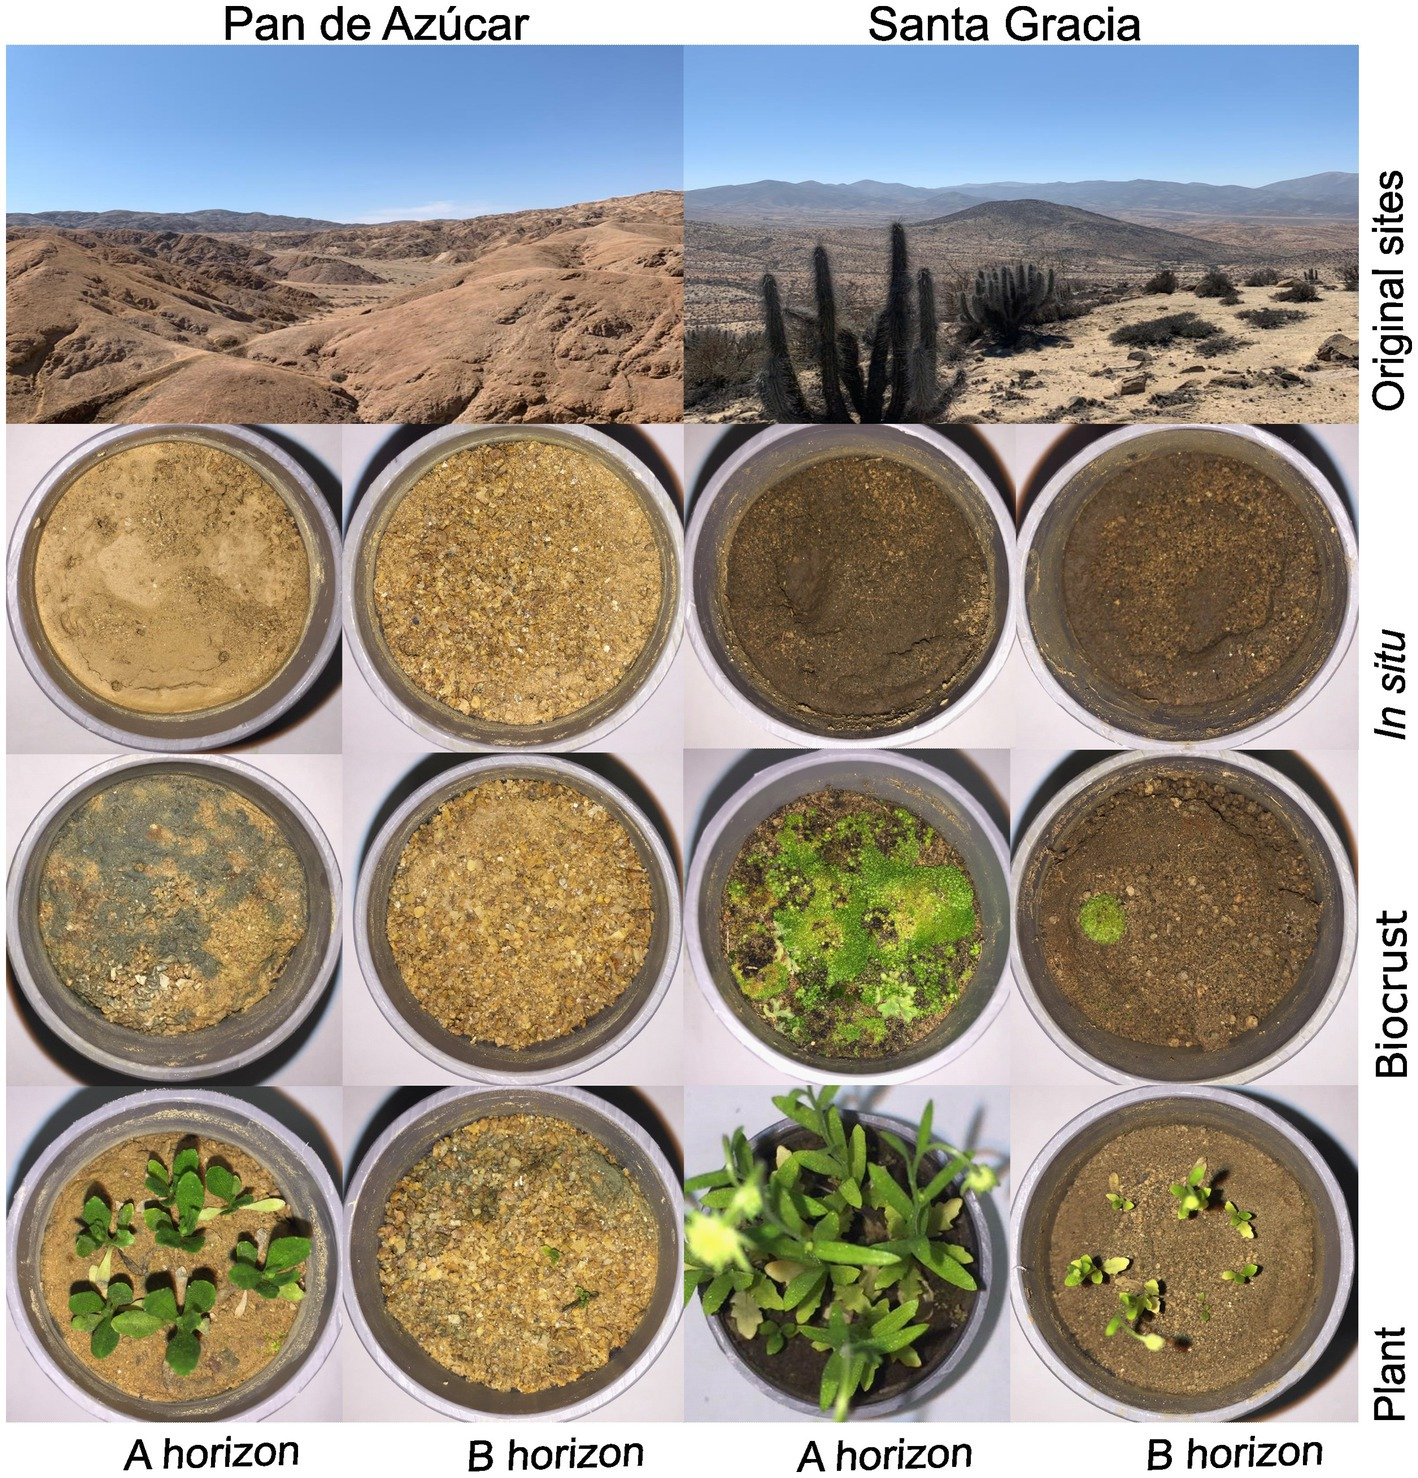
\includegraphics[width=1\textwidth]{img/M3-Figure_1.jpg}
	\caption[Sampling sites and microcosms of Pan de Azúcar and Santa Gracia after 12 weeks of incubation]{Sampling sites and microcosms of Pan de Azúcar and Santa Gracia after 12 weeks of incubation. The different microcosms are separated by horizon and treatment, including in situ, BSC (Biocrust), and plant treatment.}
	\label{fig:M3-F1}
\end{figure}

The field sampling campaign took place in March 2019, at the end of the austral summer season. The coordinates and elevations for PA were \ang{26;06;35}S, \ang{70;32;57}W, and \(\sim\)\SI{336}{\meter} elevation, while for SG, they were \ang{29;45;15}S, \ang{71;10;3}W, and \(\sim\)\SI{720}{\meter} elevation. Soil samples were taken from five plots devoid of vegetation and two soil horizons (A and B) for each site. In PA, the A horizon (PA - Ahor) ranged from \SIrange{0}{2}{\centi\metre}, and the B horizon (PA - Bhor) ranged from \SIrange{2}{25}{\centi\metre}. Similarly, in SG, the A horizon (SG - Ahor) ranged from \SIrange{0}{3}{\centi\metre}, and the B horizon (SG - Bhor) ranged from \SIrange{3}{40}{\centi\metre}. The soil structure characteristics varied between horizons. PA - Ahor exhibited a cemented crust, while PA - Bhor had a few round aggregates between coarse material, single grain dominating in the fine fraction, and gypsum concentrated in one of the plots. SG - Ahor was characterized by weak aggregates, and SG - Bhor ranged from weak to strong and stable aggregates. Fresh samples from each plot and horizon separately were homogenized through a \SI{2}{\milli\metre} sieve and stored at \SI{4}{\degreeCelsius} until use.

\subsection{Soil manipulation experiment}

An experiment was performed to stimulate initial soil formation into developed soil ecosystems by applying humid climate conditions in soil microcosms, mimicking a climate change scenario. The simulated climate change was based on the climate data of Nahuelbuta National Park in the Chilean Coastal Cordillera, where we can find well-developed deep soils with a stable soil structure \citep{Bernhard2018, RiverasMunoz2022}. As in the natural conditions of Nahuelbuta, we applied a photoperiod of \SI{14}{\hour}/\SI{10}{\hour} day/night and the daily temperature fluctuation of January (\SI{18.3}{\degreeCelsius}/\SI{11.2}{\degreeCelsius} day/night) in the soil manipulation experiment. To simulate water availability by precipitation, \SI{25}{\milli\liter} of filtered and autoclaved MiliQ water was gently applied at once three days per week until 65\% water-filled pore space was reached after each application. This value approximates the precipitation in Nahuelbuta (\SI{1469}{\milli\metre\,\year^{-1}}) but is lower due to the water retention capacity of desert soils. The microcosms consisted of \SI{130}{\gram} of field moist soil (sieved $<$\SI{2}{\milli\metre} and previously stored at \SI{4}{\degreeCelsius} for nine months) placed in sterile polyvinyl chloride columns (\SI{70}{\milli\metre} in height and \SI{50}{\milli\metre} in diameter) with a silk fabric underneath to prevent soil scattering. The microcosms were arranged on a grid inside an incubator (Memmert ICP-110, Germany), mimicking the daily temperature fluctuations. The photoperiod was set using LED-SANlight S2W (IMAGRO, Germany) and controlled with a timer coordinated with temperature fluctuations.

For the manipulation experiment setup, soil material from five plots representing top and subsoil was pooled and homogenized. The experiment included 144 microcosms representing two sites (PA and SG), two soil horizons (Ahor and Bhor), four treatments, three sampling times, and three biological replicates for each combination. In addition, three original, untreated samples were collected as baseline measurements for each site and horizon (T0), totaling 156 samples. The treatments consisted of a successional gradient of soil development as follows: (i) in situ samples with indigenous microorganisms but without BSCs or plants, (ii) in situ samples with naturally growing BSCs to assess the impact of microorganisms at a later stage of soil development, (iii) in situ samples with \textit{Helenium aromaticum} (Hook.) L.H. Bailey (pioneer plant, described below) to simulate later stages of soil development and (iv) abiotic controls based on soil sterilized samples with \ce{^{60}Co} as a source of gamma rays and a dose of \SI{50}{\kilo Gy} (BGS Beta–Gamma–Service GmbH and Co. KG, Wiehl, Germany) to exclude the impact of indigenous microorganisms. \textit{H. aromaticum} is a native vascular annual herb widely distributed in Chile, known as a pioneer plant that colonizes disturbed soils, forming seasonal grasslands \citep{GomezGonzalez2011}. For plant preparation, the seeds were sterilized using 20\% v/v sodium hypochlorite and 0.05\% Tween 20, washed three times with autoclaved MiliQ water, and placed in sterile petri dishes with absorbent paper for germination. The germinated seeds were subsequently transferred to the microcosms. BSCs occurred naturally in the soil, whereas in situ samples with microorganisms were covered with a black breathable cloth to inhibit their growth.

Microcosms were sampled at 2 weeks (T1), 12 weeks (T2), and 16 weeks (T3) of incubation. Forty eight samples were sacrificed for each sampling time, covering two sites, two soil horizons, four treatments, and three replicates. In the 12th week of sampling, the plants were harvested, and the soil with the roots was retained until the 16th week of the experiment to assess their effects on the soil. Three microcosms were transferred to a laminar flow chamber for each treatment and time point to ensure sterile conditions during sub-sampling. From the total sample, \SI{80}{\gram} of soil was collected for soil physicochemical analysis and stored in the dark at room temperature. Additionally, \SI{10}{\gram} of soil was taken for DNA extraction and held at \SI{-20}{\degreeCelsius}, while \SI{40}{\gram} was stored at \SI{-80}{\degreeCelsius} for future RNA extraction and subsequent analysis.

\subsection{Soil physicochemical properties}

To determine initial soil formation, the aggregate size distribution, and the content of total carbon (C\textsubscript{t}) and total nitrogen (N\textsubscript{t}) by aggregate size, we collected a total of 104 soil samples from three different sampling points (T0, T1, and T3). For each sample, \SI{5}{\gram} of dry soil was shaken using a modified Casagrande apparatus (Mennerich Geotechnik, Hannover, Germany). The apparatus consisted of two sieves with mesh sizes of \SI{250}{\micro\metre} and \SI{53}{\micro\metre}, placed on top of a collecting vessel. The soil samples were subjected to 1,000 repeated cycles of sieving at a frequency of \SI{2}{\hertz}, resulting in the separation of three aggregate size classes: macroaggregates (\SI{> 250}{\micro\metre}), large microaggregates (\SIrange{53}{250}{\micro\metre}), and small microaggregates and primary particles (\SI{< 53}{\micro\metre}). The data on aggregate size distribution was used to estimate aggregate stability given by the mean weight diameter of the aggregates ($\Delta$MWD) as follows:

    $$\Delta MWD = \frac{\sum_{i=1}^{n} X_i*W_i}{\sum_{i=1}^{n} W_i}$$

\(W_i\) is the corrected mass proportion of stable aggregate fraction \(i\) in the total aggregates (\SI{< 2}{\milli\metre}) and \(X_i\) is the mean diameter of stable aggregate fraction \(i\).

Subsequently, ball milling was conducted before measuring the content of C\textsubscript{t} and N\textsubscript{t} in all aggregate size classes. The process involved milling the samples for \SI{3}{\minute} at an oscillation frequency of \SI{30}{\hertz}. C\textsubscript{t} and N\textsubscript{t} measurements for all fraction samples were performed using a CHNSO elemental analyzer (HEKAtech Euro EA, Wegberg, Germany).

Additionally, we determined the total organic carbon (TOC) and total nitrogen in the bulk soil (N\textsubscript{bulk}) without aggregate size separation. This analysis used \SI{6}{\milli\gram} of bulk soil from the same subset of soil samples (104). The measurements were carried out using a flash HT 2000 Organic elemental analyzer, following a \SI{6}{M} chlorhydric acid digestion of carbonate at \SI{70}{\degreeCelsius}.

Soil pH and electrical conductivity (EC) were determined for all samples using \SI{15}{\gram} of soil. The soil pH was measured using a WTW pH 340 (WTW GmbH, Weilheim, Germany) with a Sentix 81 electrode. EC was measured using a conductivity meter (LE703, Mettler Toledo, United States). For inorganic ion analyses, \SI{5}{\gram} of each soil sample was dried for \SI{12}{\hour} at \SI{50}{\degreeCelsius} and ground to a finer consistency. Then, the leaching method described by \citet{Genderjahn2018} was employed to extract the ions from the soil. Subsequently, the resulting leachate was measured using ion chromatography (IC). The anions investigated included chloride, nitrate, phosphate, and sulfate, while the cations analyzed were sodium and calcium. Ion concentrations were calculated based on standards (Roth, Multi-Element IC-Standard Solution) using ChromStar7 software. All analyses were performed in triplicate.

\subsection{DNA extraction and quantitative PCR analysis}

TTotal genomic DNA was extracted in duplicates from \SI{0.5}{\gram} of soil for PA and \SI{0.25}{\gram} for SG using the Power Soil DNA extraction kit (Qiagen, Hilden, Germany), following the protocol described by the manufacturer. DNA extraction was exclusively performed on samples subjected to treatments involving microorganisms (in situ, biocrust, and plant treatments), resulting in a total of 116 samples. Sterile treatments devoid of biological relevance were excluded from the DNA extraction. The abundance of bacterial subunit 16S rRNA gene copies was determined by quantitative PCR (qPCR), following the procedure of \citet{Bernhard2018}. qPCR assays were performed on a CFX 96 Connect Real-Time System (Bio-rad Laboratories, CA, United States) in 96-well plates. The primers Eub341F (5\('\)-ATT ACC GCG GCT GCT GG-3\('\)) and Eub534R (5\('\)-CCT ACG GGA GGC AGC AG-3\('\)) \citep{Muyzer1993} were used. The qPCR mixture consisted of \SI{10}{\micro\liter} KAPA SYBR Fast qPCR Kit Master Mix (2x) Universal (Kapa Biosystems, Sigma-Aldrich, Germany), \SI{0.4}{\micro\liter} of each forward and reverse primer, \SI{4.2}{\micro\liter} of DNA-free water, and \SI{5}{\micro\liter} of extracted soil DNA template, resulting in a total volume of \SI{20}{\micro\liter}. The PCR conditions were as follows: initial denaturation at \SI{95}{\degreeCelsius} for \SI{3}{\minute}, followed by 40 cycles of denaturation at \SI{95}{\degreeCelsius} for \SI{3}{\second}, annealing at \SI{60}{\degreeCelsius} for \SI{20}{\second}, and elongation at \SI{72}{\degreeCelsius} for \SI{30}{\second}. We performed a melting curve analysis from \SI{65}{\degreeCelsius} to \SI{95}{\degreeCelsius}, with an increment of \SI{0.5}{\degreeCelsius} to ensure the qPCR specificity. We used standard curves from a known number of PCR-amplified target genes of a pure culture of \textit{Escherichia coli} to estimate the unknown bacterial abundance. All the samples were analyzed in three replicate reactions.

\subsection{Sequencing}

For sequencing, DNA extracted from each sample was amplified using the primer pair 515F (5\('\)-\texttt{GTG YCA GCM GCC GCG GTA A}-3\('\)) and 806R (5\('\)-\texttt{GGA CTA CNV GGG TWT CTA AT}-3\('\)), targeting the V4 hypervariable regions of the bacterial 16S rRNA gene \citep{Apprill2015, Parada2016} including additional barcodes. The polymerase chain reactions were performed in triplicate in a total volume of \SI{25}{\micro\liter}, following the conditions described in \citet{Rodriguez2022} with modifications (reducing the number of denaturation cycles to 20 instead of 30). To confirm the amplification success, PCR products were analyzed by electrophoresis in \SI{1.5}{\percent} agarose gels stained with Gelred\textsuperscript{TM} Nucleic acid gel stain (Biotium, United States). The triplicate PCR samples were pooled and then purified using the carboxyl-coated magnetic beads (Agencourt\textsuperscript{\textregistered} AMPure\textsuperscript{\textregistered} XP Kit, Beckman Coulter, Brea, CA, United States). The purified DNA was quantified using the Qubit Fluorometer (Invitrogen\textsuperscript{TM}, Thermo Fisher Scientific, United States). For sequencing, all PCR products were pooled in equal concentrations of \SI{20}{\nano\gram} for Paired-end sequencing ($2\times 300$\,bp) at Eurofins (Eurofins Genomics Europe Shared Services GmbH, Ebersberg, Germany).

\subsection{Processing of 16S rRNA data}

To generate the amplicon sequence variants (ASVs), the sequencing library was first demultiplexed using cutadapt v3.4 \citep{Martin2011} with the following parameters: \texttt{-e 0.2 -q 15,15 -m 150 --discard-untrimmed}. Only read pairs with the correct barcodes at both ends were retained for further analysis. Next, the DADA2 package v1.20 \citep{Callahan2016} in R v4.1 was employed to generate ASVs from the trimmed reads using a pooled approach with the following parameters: \texttt{truncLen = c(240,200), maxN = 0, rm.phix = TRUE, minLen = 200}. Taxonomic assignment was performed using DADA2 and the SILVA database v138 \citep{Quast2012}. To filter out non-target sequences, ASVs representing chloroplasts, mitochondria, and singletons were removed from the dataset. The raw Illumina sequencing data have been deposited at the European Nucleotide Archive under the BioProject ID \texttt{PRJEB60029}.

\subsection{Data analysis}

All statistical analyses were conducted in R Studio v4.0.5. We performed the Kruskal-Wallis test to determine differences in soil properties, the relative abundance of 16S rRNA, and diversity indices. Post-hoc pairwise comparisons were performed using the Mann–Whitney test, with \(p\)-values adjusted using the Bonferroni correction for multiple comparisons.

To minimize bias due to sequencing depth, all samples were rarefied to 12,000 reads per sample using the \texttt{rtk} package \citep{Saary2017}. Alpha diversity indices, including the Shannon index, observed species, and evenness, were calculated using the \texttt{vegan} package \citep{Oksanen2013}. Relative abundances were calculated by transforming absolute read numbers, and soil physicochemical properties were normalized by subtracting the mean and dividing by the standard deviation. Nonmetric multidimensional scaling (NMDS) with Bray-Curtis distance dissimilarity was performed to assess differences in bacterial structure. The significance of differences between sites, horizon, and time was estimated using PERMANOVA (\texttt{adonis} function) and post-hoc pairwise comparisons (\texttt{pairwise.adonis}) from the \texttt{pairwiseAdonis} package \citep{MartinezArbizu2017} with a significance of \(p < 0.05\). Soil properties influencing bacterial composition were determined using distance-based redundancy analysis (dbRDA) with the \texttt{capscale} function in \texttt{vegan}. The multicollinearity of these variables was examined using the variance inflation factor (VIF), and values \(>10\) were removed. Finally, the FAPROTAX database \citep{Louca2016} was used to analyze the whole bacterial community and predict function from taxonomy.

Correlation analyses between molecular analysis and soil properties were performed using Pearson correlation (\(p < 0.05\)). The results were visualized using the \texttt{ggplot2} package \citep{Wickham2011}.

For further analyses, only abundant ASVs with a proportion of total sequences greater than \SI{0.05}{\percent} were retained to reduce underrepresented ASVs and table complexity. Indicator species were identified using the \texttt{indval} function in the \texttt{labdsv} package to find ASVs leading to changes in multivariate patterns \citep{Roberts2016}. Associations were considered significant with an R-value of 0.8 (\(p < 0.05\)). Then, a network analysis was conducted to understand the distribution patterns of bacterial assemblages using a simplified version of the ecological interactions \citep{Barberan2012, Qian2018}. The co-occurrence network was constructed using the \texttt{igraph} package \citep{Csardi2006} and visualized through the Fruchterman-Reingold layout. Pairwise correlations among ASVs were calculated using the \texttt{rcorr} function within the \texttt{Hmisc} package \citep{Harrell2019}. A Pearson correlation coefficient of R-value \(>0.7\) (\(p < 0.01\)) between two ASVs was considered statistically robust. Topological properties of the network, such as the number of nodes and edges, clustering coefficient, average degree, connectance, and modularity, were calculated using the \texttt{igraph} package. Furthermore, clusters of highly correlated ASVs were grouped into modules using the \texttt{WGCNA} package \citep{Langfelder2008}, and their associations with physicochemical properties were explored. Highly connected nodes (hub ASVs) were then identified from each module.

\section{Results}
\subsection{Soil manipulation experiment}

The microcosms represent a successional gradient of soil development divided into three biological treatments (\ref{fig:M3-F1}: soil with \textit{in situ} microorganisms (\textit{in situ}), soil with \textit{in situ} microorganisms and BSCs (BSC), and soil with \textit{in situ} microorganisms and plants (plant). The \textit{in situ} treatment had no plant growth or BSC development, similar to the sterile treatment. In the BSC treatment, varying types and coverage were observed among sites and horizons. Specifically, a leaden BSC developed in PA, while a greenish BSC formed in SG in both horizons. The A horizons of both sites showed nearly complete coverage of the microcosms with BSCs. In contrast, the B horizons showed patchy coverage without forming a compact or extended layer of BSC on the surface. Regarding the plant treatments, similar patterns were observed. In PA, the roots were light brown, and the biomass (both below- and aboveground) and vegetative development were comparatively lower than in SG. In contrast, SG showed dark brown roots, higher biomass, and reached the flowering stage in both horizons. In the PA-Ahor, plants with numerous lateral roots ranged from \SIrange{2}{3}{\centi\metre} in height. Conversely, in PA–Bhor, plants were less than \SI{5}{\milli\metre} tall, had a short taproot with few lateral roots, and experienced a mortality rate of over \SI{50}{\percent} after seven weeks. In SG–Ahor, flowering plants with heights ranging from \SIrange{11}{14}{\centi\metre} were observed. These plants had a \SI{7}{\centi\metre} long taproot and numerous lateral roots covering completely the microcosms. On the other hand, SG–Bhor exhibited plants ranging from \SIrange{1}{3}{\centi\metre} in height, with flower buds and roots reaching \SI{5}{\centi\metre} in length with fewer lateral roots than SG–Ahor. After removing the plants at 12 weeks, no visual differences were observed in the roots between weeks 12 and 16, which remained compact and defined with no signs of degradation. Given the intact nature of the roots during this period, it is considered that these conditions did not impact the short-term degradation of this organic material. Overall, the differences between treatments were less pronounced in the B horizons than in the A horizons, indicating more favorable conditions for BSC and plant development in the A horizons.

\subsection{Soil physical and chemical properties}

Soil samples were analyzed to determine the mass distribution of macro- and microaggregates and the concentrations of C\textsubscript{t} and N\textsubscript{t} in each soil aggregate size. No significant differences in aggregate size distribution were found between the study sites (PA--SG; \(n = 54\)), with average proportions of \SI{67}{\percent} macroaggregates, \SI{27}{\percent} large microaggregates, and \SI{7}{\percent} small microaggregates. However, significant differences existed between horizons within each site (Ahor--Bhor; \(n = 27\), \(p < 0.01\)). In both sites, the proportion of macroaggregates was highest in the B horizon, while microaggregates dominated the A horizon. Specifically, macroaggregates mean values were \SI{54}{\percent} in PA--Ahor, \SI{81}{\percent} in PA--Bhor, \SI{63}{\percent} in SG--Ahor, and \SI{70}{\percent} in SG--Bhor. For microaggregates, the means were \SI{23}{\percent} in PA--Ahor, \SI{9}{\percent} in PA--Bhor, \SI{19}{\percent} in SG--Ahor, and \SI{15}{\percent} in SG--Bhor. Significant differences in the concentration of C\textsubscript{t} and N\textsubscript{t} were observed between sites and horizons (\(p < 0.01\)). C\textsubscript{t} was higher in macro- and large microaggregates of PA (mean \SI{1.2}{\percent}) than in SG (mean \SI{0.7}{\percent}), while N\textsubscript{t} was significantly higher in macro- and microaggregates of SG (mean \SI{0.08}{\percent}) than in PA (mean \SI{0.03}{\percent}). Analysis between horizons showed that macro- and microaggregates of PA--Bhor had a higher C\textsubscript{t} mean of \SI{2}{\percent} than PA--Ahor’s \SI{0.8}{\percent}. Conversely, SG--Ahor’s macro- and large microaggregates had a higher C\textsubscript{t} mean of \SI{1.1}{\percent} than SG--Bhor’s \SI{0.8}{\percent}. In terms of N\textsubscript{t}, higher percentages were observed in SG--Ahor (mean \SI{0.1}{\percent}) and PA--Ahor (mean \SI{0.033}{\percent}) than in SG--Bhor (mean \SI{0.07}{\percent}) and PA--Bhor (mean \SI{0.026}{\percent}).

Over time, we observed changes in aggregate size distribution as well as in C\textsubscript{t} and N\textsubscript{t} concentrations. In PA--Ahor, the C\textsubscript{t} of large microaggregates decreased from \SI{0.93}{\percent} in T0 to \SI{0.83}{\percent} in T3. In PA--Bhor, the proportion of macroaggregates increased from \SI{67}{\percent} to \SI{81}{\percent}, while for large microaggregates decreased from \SI{28}{\percent} to \SI{14}{\percent} between T0 and T3. Consequently, MWD increased from \SI{0.8}{\milli\metre} in T0 to \SI{0.94}{\milli\metre} in T3. In SG--Ahor, no marked contrast was observed from T0 to T3, while in SG--Bhor, the percentage of C\textsubscript{t} in macroaggregates increased from \SI{0.2}{\percent} to \SI{0.3}{\percent} over time. Regarding differences between treatments, microorganism-plant treatments showed a noticeable increase in macroaggregates and, thus, in MWD compared to the sterile treatments at T3 (\ref{fig:M3-F2}). The MWD values for sterile compared to plant treatments were as follows: PA--Ahor (mean \SI{0.7}{mm} vs. \SI{0.78}{\milli\metre}), PA--Bhor (mean \SI{0.91}{mm} vs. \SI{0.95}{\milli\metre}), SG--Ahor (mean \SI{0.75}{mm} vs. \SI{0.87}{\milli\metre}), and SG--Bhor (mean \SI{0.87}{mm} vs. \SI{0.89}{\milli\metre}).

Regarding TOC and N\textsubscript{bulk} (without aggregate size separation) in the bulk soil samples, SG exhibited significantly higher levels (\SI{0.7}{\percent} and \SI{0.06}{\percent}, respectively) than PA (\SI{0.1}{\percent} and \SI{0.02}{\percent}, respectively). When considering the horizons, both N\textsubscript{bulk} and TOC were significantly higher in PA--Ahor (\SI{0.03}{\percent} and \SI{0.14}{\percent}, respectively) and SG--Ahor (\SI{0.08}{\percent} and \SI{0.9}{\percent}, respectively) than PA--Bhor (\SI{0.01}{\percent} and \SI{0.06}{\percent}, respectively) and SG--Bhor (\SI{0.04}{\percent} and \SI{0.46}{\percent}, respectively). Over time, a notable increase in TOC was observed only in SG--Bhor, rising from \SI{0.32}{\percent} in T0 to \SI{0.48}{\percent} in T3. No clear trends were identified for the treatments (\ref{fig:M3-F2}).

\begin{figure}[H]
	\centering
	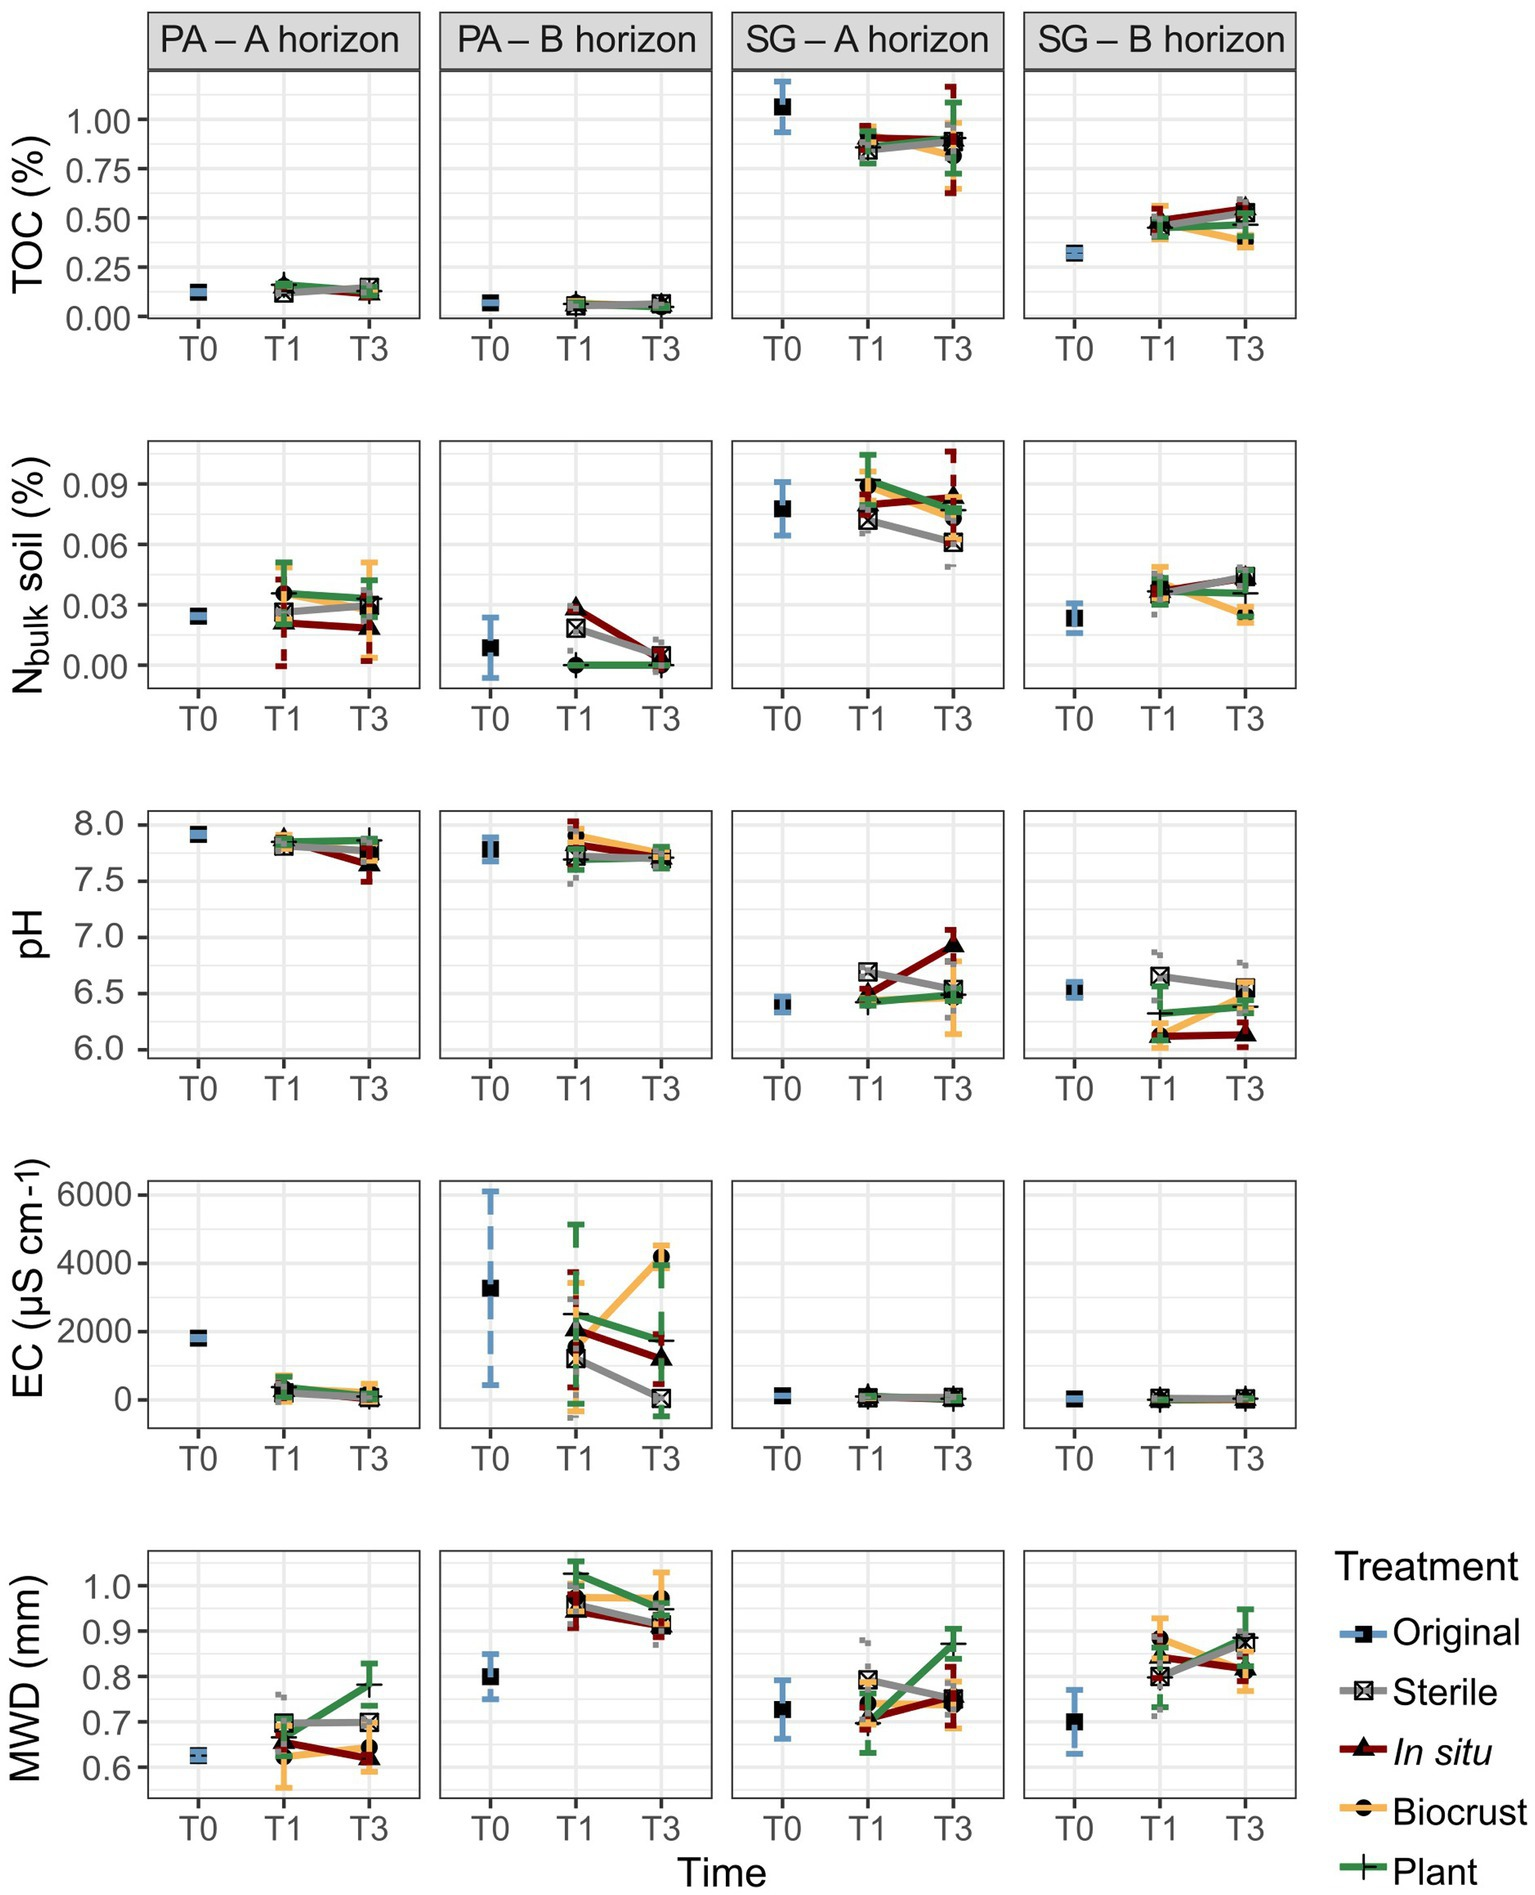
\includegraphics[width=1\textwidth]{img/M3-Figure_2.jpg}
	\caption[Physicochemical properties in Pan de Azúcar and Santa Gracia]{Physicochemical properties in Pan de Azúcar (PA) and Santa Gracia (SG) show total organic carbon (TOC), nitrogen in bulk soil (Nbulk), pH, electrical conductivity (EC), and mean weight diameter (MWD) in three-time points of the soil manipulation experiment. Time is represented by T0 (original soil sample), T1 (2 weeks), and T3 (16 weeks). Different colors represent the different treatments. Each bar is the mean of biological triplicates.}
	\label{fig:M3-F2}
\end{figure}

The results revealed significant differences in soil pH, EC, and ion concentrations among the studied sites and horizons (\(p < 0.01\); \ref{fig:M3-F2}). Specifically, in PA, higher values were observed for pH (mean 7.8), EC (mean \SI{1272}{\micro\siemens\per\centi\metre}), sodium (mean \SI{93.4}{\milli\gram\per\liter}), chloride (mean \SI{160.2}{\milli\gram\per\liter}), and sulfate (mean \SI{783.6}{\milli\gram\per\liter}) compared to SG, where the respective mean values were 6.5, \SI{51.8}{\micro\siemens\per\centi\metre}, \SI{5.5}{\milli\gram\per\liter}, \SI{6.2}{\milli\gram\per\liter}, and \SI{1.4}{\milli\gram\per\liter}. Furthermore, significant differences in soil parameters were found between soil horizons. PA--Bhor exhibited higher EC (mean \SI{2186}{\micro\siemens\per\centi\metre}), sodium (mean \SI{141}{\milli\gram\per\liter}), chloride (mean \SI{246.7}{\milli\gram\per\liter}), calcium (mean \SI{630}{\milli\gram\per\liter}), and sulfate (mean \SI{1532.6}{\milli\gram\per\liter}) concentrations than PA--Ahor, where the respective mean values were \SI{359}{\micro\siemens\per\centi\metre}, \SI{45.8}{\milli\gram\per\liter}, \SI{73.8}{\milli\gram\per\liter}, \SI{12.5}{\milli\gram\per\liter}, and \SI{14.8}{\milli\gram\per\liter}. In SG, higher pH and EC were observed in the A horizon (mean 6.6 and \SI{63}{\micro\siemens\per\centi\metre}, respectively) than in the B horizon (mean 6.4 and \SI{41}{\micro\siemens\per\centi\metre}, respectively). Additionally, changes over time were observed, with substantial decreases of EC (from \num{1809} to \num{103.7}\,\si{\micro\siemens\per\centi\metre}), sodium (from \num{108.8} to \SI{32.7}{\milli\gram\per\liter}), and chloride (from \num{265.3} to \SI{48.2}{\milli\gram\per\liter}) concentrations from T0 to T3 in PA--Ahor. PA--Bhor also showed a marked decrease in sodium and chloride concentration from \num{250.2} and \SI{522.6}{\milli\gram\per\liter} to \num{109} and \SI{164.5}{\milli\gram\per\liter}, respectively. 
No remarkable changes were found for the horizons of SG over time, as well as for treatments in PA or SG.

\subsection{Bacterial abundance}

The bacterial gene copy numbers are shown in \ref{fig:M3-F3}. A significantly higher gene copy number for bacteria was observed in SG, ranging from \num{e7} to \num{e8}~gene copies\,\si{\gram^{-1}} soil, compared to PA, ranging from \num{e5} to \num{e7}~gene copies\,\si{\gram^{-1}} soil. Comparison between soil horizons showed significantly higher gene copy numbers in the A horizon for both sites. The mean of gene copies\,\si{\gram^{-1}} soil for PA--Ahor was \num{4.5e7} and for PA--Bhor \num{1.2e6}, while for SG--Ahor was \num{3.9e8} and for SG--Bhor \num{9.2e7}. Considering the times evaluated, both horizons in PA showed an increase in the gene copy numbers from T0 (mean of gene copies\,\si{\gram^{-1}} soil for Ahor \num{1.9e7} and Bhor \num{8.3e5}) to T3 (mean of gene copies\,\si{\gram^{-1}} soil for Ahor \num{4.7e7} and Bhor \num{1.1e6}). In contrast, SG decreased the gene copy number over time in both horizons. The mean of gene copy\,\si{\gram^{-1}} soil for SG--Ahor decreased from \num{5e8} in T0 to \num{2.9e8} in T3, while SG--Bhor reduced from \num{1.8e8} in T0 to \num{8.2e7} in T3. There were no discernible patterns between treatments. The gene copy numbers correlated positively with N\textsubscript{t} in all aggregate classes, N\textsubscript{bulk} and TOC (\(R > 0.7\)), and negatively with pH (\(R = 0.6\)).

\begin{figure}[H]
	\centering
	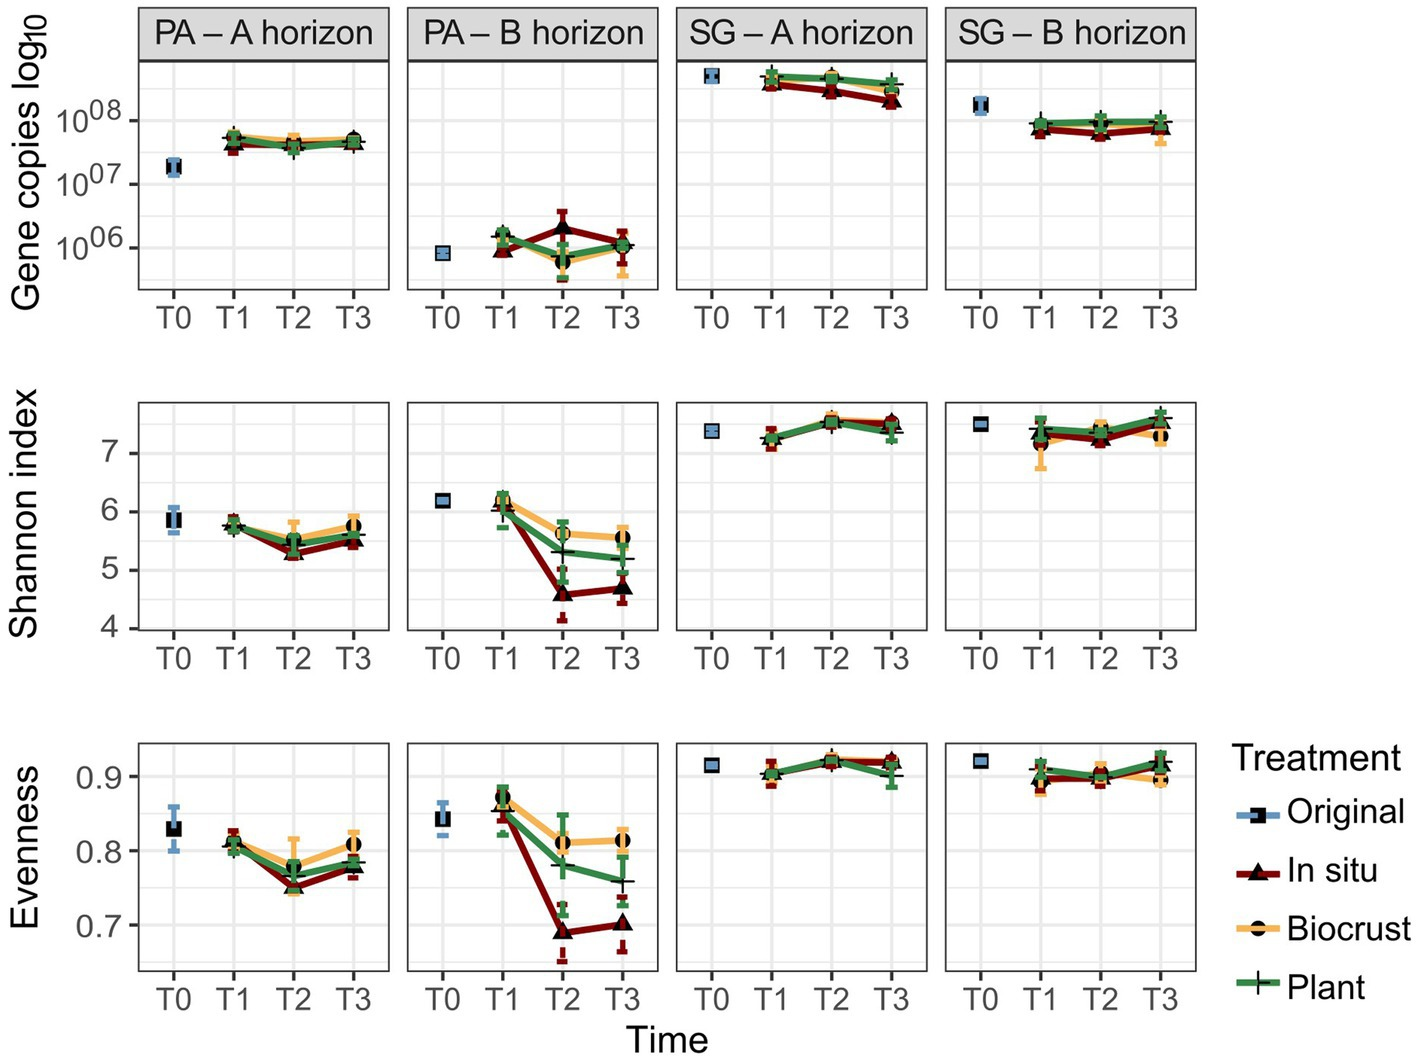
\includegraphics[width=1\textwidth]{img/M3-Figure_3.jpg}
	\caption[Gene copy numbers, Shannon index, and Evenness of bacterial communities in Pan de Azúcar and Santa Gracia in four soil manipulation experiment time points]{Gene copy numbers, Shannon index, and Evenness of bacterial communities in Pan de Azúcar (PA) and Santa Gracia (SG) in four soil manipulation experiment time points. Time is represented by T0 (original), T1 (2 weeks), T2 (12 weeks), and T3 (16 weeks). Different colors represent the different treatments. Each bar is the mean of biological triplicates.}
	\label{fig:M3-F3}
\end{figure}

\subsection{Alpha and beta diversity}

Sequencing analysis of 116 soil samples yielded 4.3 million raw reads, of which 3.1 million (\SI{72.7}{\percent} of the total) were retained after filtering, merging, and removing chimera. These reads were assigned to bacteria (\SI{98.5}{\percent}), archaea (\SI{1.3}{\percent}), or unclassified (\SI{0.2}{\percent}) groups. Since the percentage of archaea was low (with a mean of 594 reads per sample), only bacterial data were analyzed. The number of reads per bacterial sample ranged from \num{12178} to \num{275292}, with a mean of \num{90155} reads per sample. Considering the minimum read number, the samples were rarified to 12,000 reads. The final dataset contained \num{24465} amplicon sequence variants (ASVs) and \num{1108} putative genera.

This study evaluated the alpha-diversity indices, including the Shannon index, observed species, and evenness (\ref{fig:M3-F3}. The results revealed significant differences between PA and SG, with SG exhibiting higher values for all three indices. The Shannon index ranged from 4.1 to 6.3 in PA, while SG showed values ranging from 6.7 to 7.7. A similar trend was noticed for the observed species, with PA ranging from 550 to 1,754 and SG ranging from 2,075 to 4,029. For evenness, values varied between 0.87 to 0.93 in SG and 0.64 to 0.88 in PA. For the soil horizons, only the observed species values showed significant differences. PA--Ahor had a higher mean of 1,215 compared to 1,050 in PA--Bhor, whereas SG--Bhor showed a mean of 3,541 compared to 3,389 in SG--Ahor. Over time, greater changes were observed in both horizons of PA. Samples analyzed at T0 in PA--Ahor showed a marked decrease in the Shannon index and evenness at T2. The mean Shannon index decreased from 5.9 to 5.4, while evenness decreased from a mean of 0.83 to 0.76 in the same period. In PA--Bhor, the Shannon index, evenness, and observed species prominently reduced from T0 to T3. The mean Shannon index decreased from 6.2 to 5.1, evenness from 0.84 to 0.76, and the observed species mean varied from 1,568 in T0 to 892 in T3. No robust differences were observed between time or treatments in SG. However, in PA--Bhor, the Shannon index showed considerable disparities between treatments at T3, with the lowest values observed in the \textit{in situ} treatment (4.7), followed by plants (5.2) and BSC (5.6).

Correlations between alpha diversity indices and soil properties were examined, revealing a positive correlation between the Shannon index and the observed species with N\textsubscript{t} across all aggregate sizes, N\textsubscript{bulk}, and TOC (\(R > 0.6\)). Conversely, a negative correlation was observed with sodium, sulfate (\(R < -0.6\)), and pH (\(R < -0.9\)).

Analysis of NMDS showed the patterns of change in the bacterial community, and PERMANOVA allowed the calculation of the statistical differences associated with these changes. The statistical analysis revealed that bacterial composition was significantly different between the sites (PA vs. SG) and between the horizons (Ahor vs. Bhor; \(p < 0.01\)). In addition, it became visible that climate manipulation had changed the bacterial community over time (\(n=9\), \(p < 0.05\)). For both PA--Ahor and PA--Bhor, T1 was significantly different from T2 and T3. In SG--Ahor, T1 differed significantly from T3, while SG--Bhor showed no change over time. Statistical analysis with T0 was not possible due to the small number of samples (\(n=2\)). PA--Ahor, PA--Bhor, and SG--Ahor treatments showed increasing disparity, transitioning from initial similarity to marked dissimilarity among the treatments as time progressed.

We employed a dbRDA model to assess the influence of soil parameters on the variation in bacterial composition (\ref{fig:M3-F4}). In PA--Ahor, the bacterial composition showed positive correlations with EC at T0, N\textsubscript{t} in microaggregates at T1, and MWD at T3, collectively explaining \SI{38.9}{\percent} of the total variation. At T3, differentiation between treatments became apparent. PA--Bhor exhibited positive associations with sodium at T0, C\textsubscript{t} in macroaggregates at T1, and C\textsubscript{t} in small microaggregates at T3, explaining \SI{40.4}{\percent} of the total variation. In SG--Ahor, higher EC at T0 and T1 displayed a positive association, while treatments began to differentiate at T3. Notably, a distinct positive trend was observed between N\textsubscript{t} in macroaggregates and the plant treatment, while \textit{in situ} and BSC treatments were linked to higher pH. These variables accounted for \SI{22.2}{\percent} of the total variation. In SG--Bhor, the variables explained \SI{17.2}{\percent} of the total variation, and no discernible patterns were found to differentiate between times or treatments regarding N\textsubscript{t} in macroaggregates, TOC, or EC.

\begin{figure}[H]
	\centering
	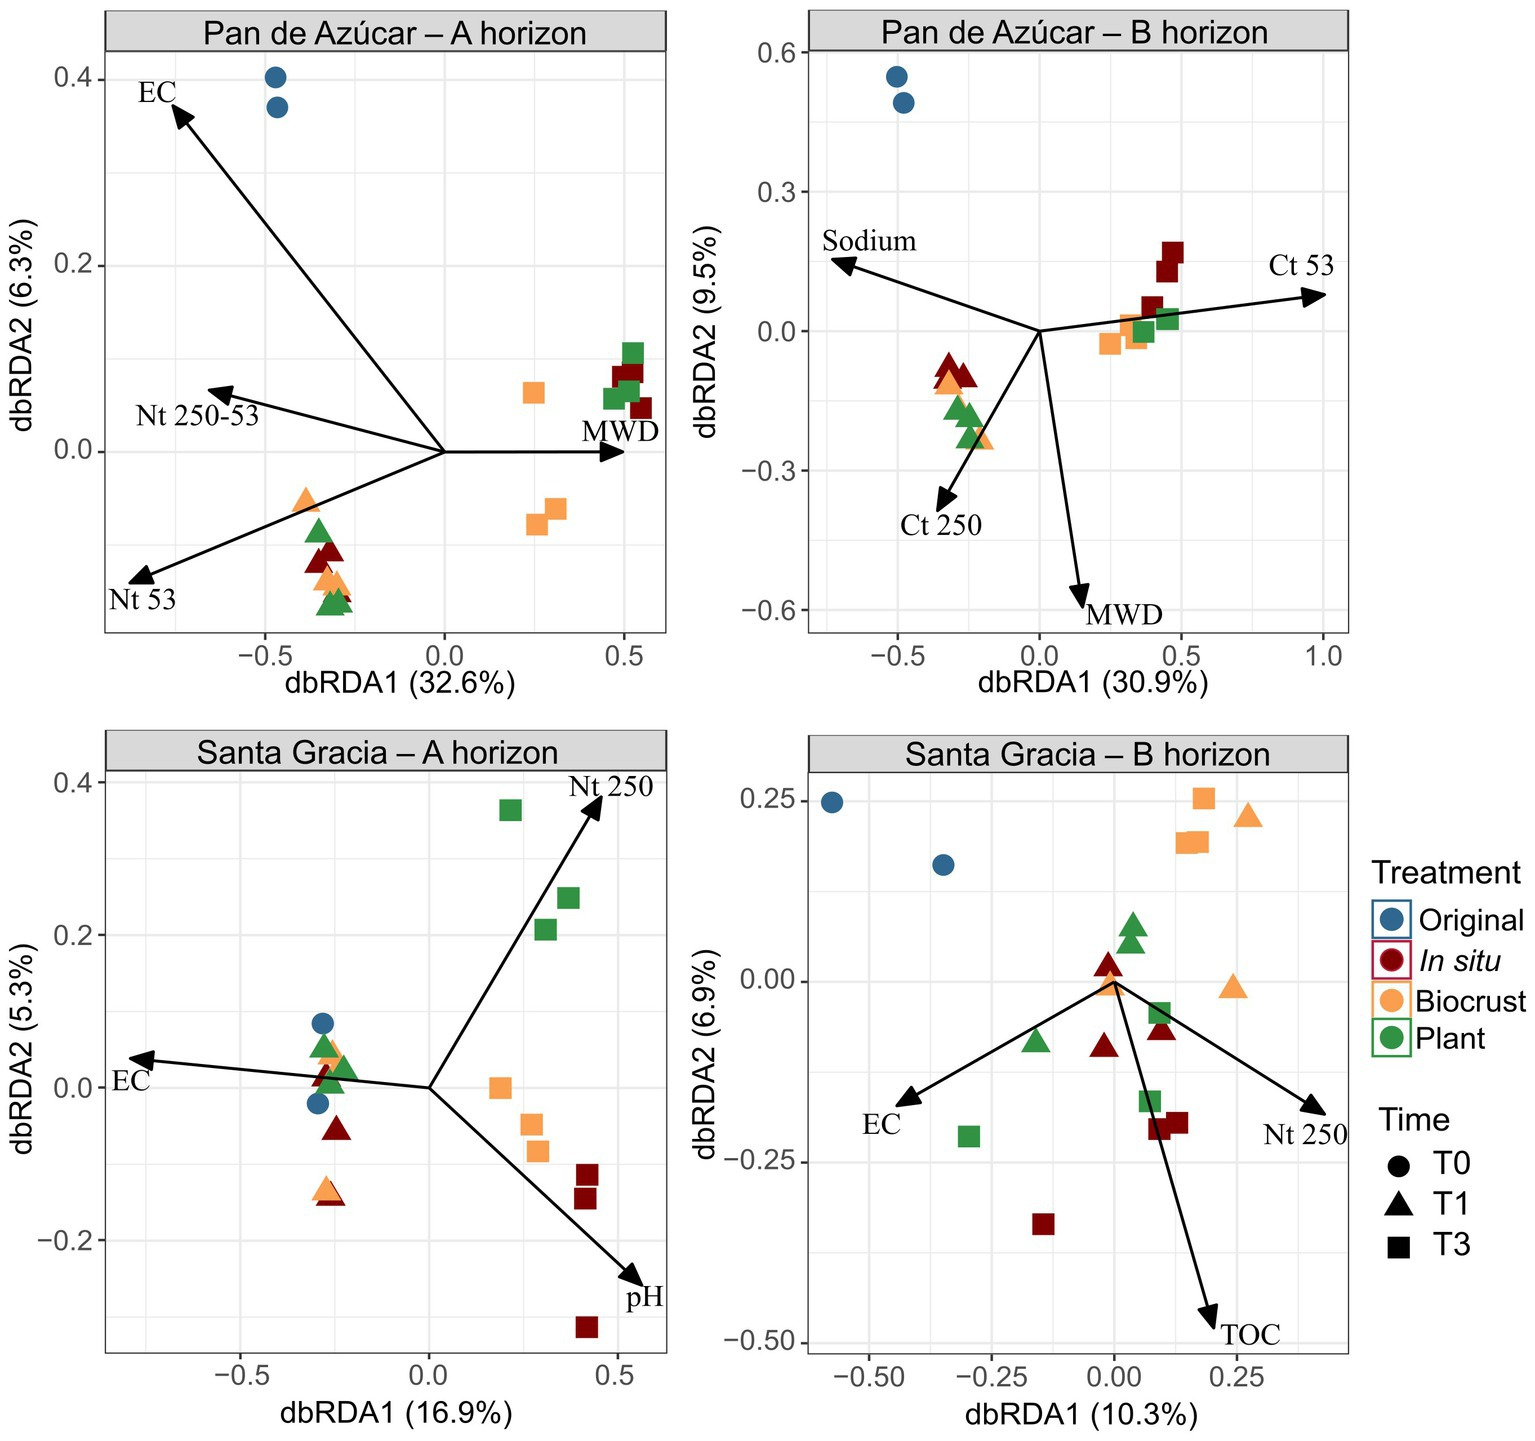
\includegraphics[width=1\textwidth]{img/M3-Figure_4.jpg}
	\caption[Distance-based redundancy analysis (dbRDA) including soil properties for A and B soil horizons in Pan de Azúcar and Santa Gracia]{Distance-based redundancy analysis (dbRDA) including soil properties for Pan de Azúcar - A horizon, Pan de Azúcar - B horizon, Santa Gracia - A horizon, and Santa Gracia - B horizon. Significant physicochemical properties included total organic carbon (TOC), nitrogen in macroaggregates (Nt 250), nitrogen in large microaggregates (Nt 250-53), nitrogen in small microaggregates (Nt 53), pH, electrical conductivity (EC), sodium, mean weight diameter (MWD), total carbon in macroaggregates (Ct 250), total carbon in small microaggregates (Ct 53). Time is represented by T0 (original soil sample), T1 (2 weeks), and T3 (16 weeks). Different color represents different treatments, while shapes represent different sampling times. Each point is the mean of biological triplicates.}
	\label{fig:M3-F4}
\end{figure}

\subsection{Change in bacterial community composition}

The analysis of relative bacterial abundances per site revealed that Proteobacteria (\SI{27.2}{\percent}), Actinobacteriota (\SI{12.9}{\percent}), and Gemmatimonadota (\SI{10.5}{\percent}) were the most abundant phyla in PA, while Acidobacteriota (\SI{20.7}{\percent}), Proteobacteria (\SI{20.5}{\percent}), and Planctomycetota (\SI{11.8}{\percent}) dominated in SG. The phyla distribution varied significantly between horizons in both sites (\ref{fig:M3-F5}). In PA, Acidobacteriota and Proteobacteria were more abundant in PA--Ahor (\SI{5.4}{\percent} and \SI{31.9}{\percent}, respectively) than in PA--Bhor (\SI{1.9}{\percent} and \SI{22.6}{\percent}, respectively), while Actinobacteriota and Firmicutes dominated the PA--Bhor (\SI{16.7}{\percent} and \SI{10.3}{\percent}, respectively) compared to PA--Ahor (\SI{9.1}{\percent} and \SI{0.8}{\percent}, respectively). In SG, Proteobacteria and Bacteroidetes were more abundant in SG--Ahor (\SI{25.8}{\percent} and \SI{12.2}{\percent}, respectively) than in SG--Bhor (\SI{15.3}{\percent} and \SI{5.2}{\percent}, respectively). Acidobacteriota and Verrucomicrobiota were more abundant in SG--Bhor (\SI{27.1}{\percent} and \SI{10.9}{\percent}, respectively) than in SG--Ahor (\SI{14.3}{\percent} and \SI{6.2}{\percent}, respectively). In addition, some taxa became dominant or scarce over time. For instance, a substantial increase was observed in Proteobacteria from T0 to T3, rising from \SI{9.4}{\percent} to \SI{35}{\percent} in the A horizon and from \SI{13.7}{\percent} to \SI{27.7}{\percent} in the B horizon. Moreover, there were increases in Planctomycetota and Bacteroidota in both horizons. In contrast, Actinobacteriota decreased significantly from T0 to T3 in PA--Ahor (\SI{34.5}{\percent} to \SI{5.6}{\percent}) and PA--Bhor (\SI{51.5}{\percent} to \SI{13.1}{\percent}). In contrast to PA, in SG--Ahor, the community exhibited variable changes but remained consistently dominated by the three most abundant taxa, Acidobacteriota (\SI{14.3}{\percent}), Proteobacteria (\SI{25.8}{\percent}), and Planctomycetota (\SI{13.2}{\percent}). SG--Bhor is characterized by the dominance of Acidobacteriota (\SI{27.1}{\percent}) and Proteobacteria (\SI{15.3}{\percent}), which remained stable, while Actinobacteriota exhibited a decrease from \SI{25.9}{\percent} to \SI{9.2}{\percent}, being replaced by Planctomycetota. Finally, no clear trends in bacterial phyla abundance between SG treatments were observed. Still, PA--Ahor showed an increased abundance of Acidobacteriota and Planctomycetota in plant treatment (\SI{12.7}{\percent} and \SI{15.5}{\percent}, respectively) compared to \textit{in situ} treatment (\SI{5.9}{\percent} and \SI{6.8}{\percent}, respectively).

\begin{figure}[H]
	\centering
	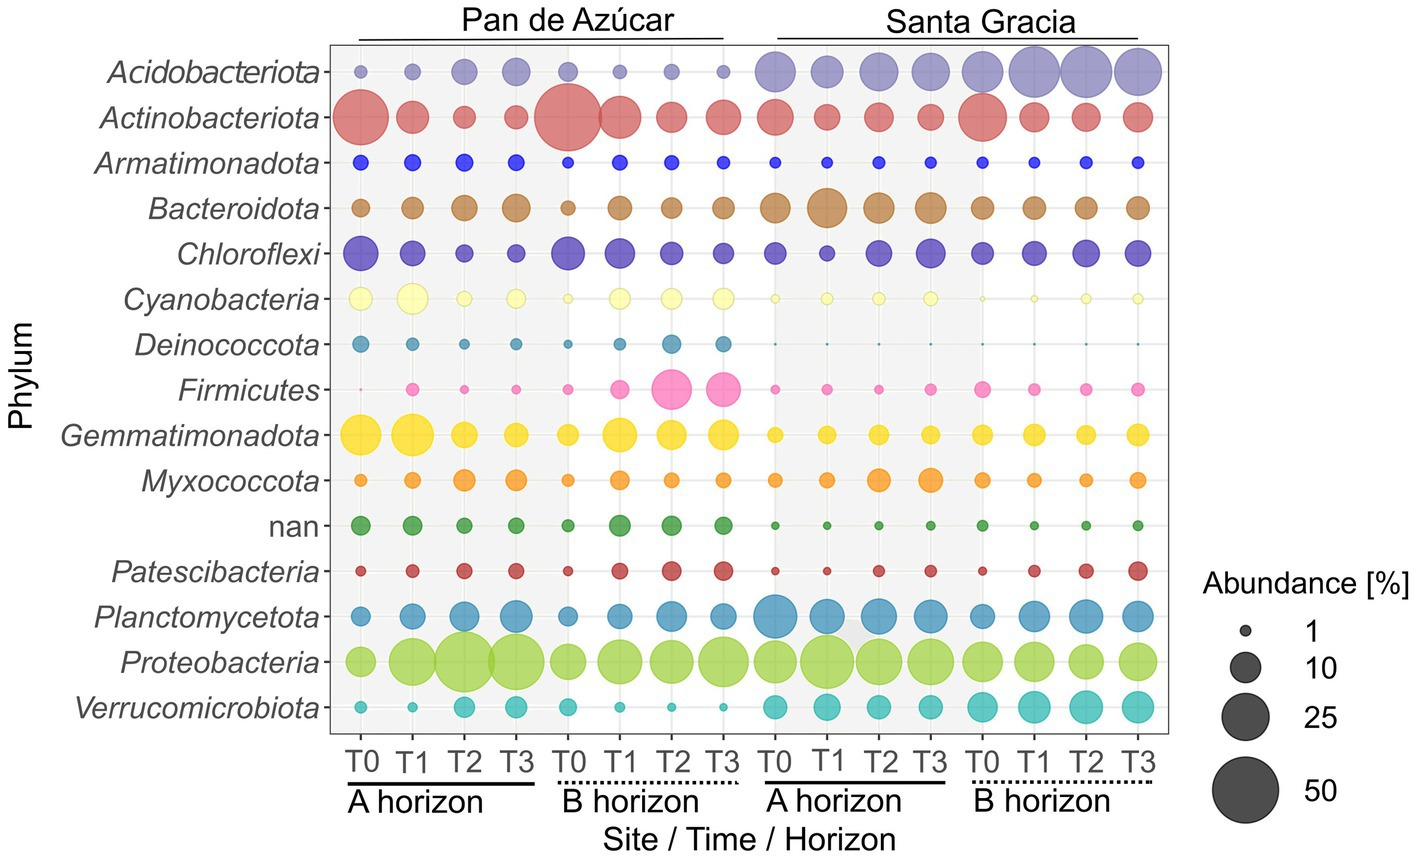
\includegraphics[width=1\textwidth]{img/M3-Figure_5.jpg}
	\caption[Relative abundance of top 15 bacterial phyla for Pan de Azúcar and Santa Gracia in four-time points of the soil manipulation experiment]{Relative abundance of top 15 bacterial phyla for Pan de Azúcar and Santa Gracia in four-time points of the soil manipulation experiment. Time is represented as T0 (original), T1 (2 weeks), T2 (12 weeks), and T3 (16 weeks). Each bubble is the mean of the different treatments (in situ, BSCs, and plants) and biological triplicates.}
	\label{fig:M3-F5}
\end{figure}

Correlations between the most abundant bacterial phyla and soil properties were observed. Acidobacteriota and Verrucomicrobia showed a positive correlation with N\textsubscript{t} in small microaggregates (\(R=0.7\)) and a negative correlation with C\textsubscript{t} in macroaggregates and pH (\(R=-0.8\)), as well as with sodium and sulfate (\(R < -0.6\)). Conversely, Gemmatimonadota showed a positive correlation with C\textsubscript{t} in macroaggregates and pH (\(R=0.5\)) but a negative correlation with N\textsubscript{t} in microaggregates and TOC (\(R < -0.6\)). Actinobacteriota positively correlated with sodium and chloride (\(R=0.6\)), while Bacteroidota correlated with N\textsubscript{t} in large microaggregates, N\textsubscript{bulk}, and TOC (\(R > 0.6\)).

\subsection{Change in potential predicted functions}

Nine thousand two hundred ASVs (\num{9200}) were assigned to 37 ecologically relevant functions described in FAPROTAX. The two most prevalent functions across all microcosms were chemoheterotrophy (electron acceptor is variable) and aerobic chemoheterotrophy (electron acceptor is O\textsubscript{2}), comprising a mean of \SI{48.2}{\percent} and \SI{30.2}{\percent} of the taxonomic abundance in PA and SG, respectively. Additionally, PA showed other abundant functions such as nitrate reduction, phototrophy-associated functions (phototrophy, photoautotrophy, photosynthetic cyanobacteria, and oxygenic photoautotrophy), and functions associated with degradation processes (hydrocarbon degradation, aromatic compound degradation, aromatic hydrocarbon degradation, and aliphatic non-methane hydrocarbon degradation), with a mean of \SI{24}{\percent} of taxonomic abundance. In contrast, SG exhibited nitrate reduction, ureolysis, and fermentation, with a mean taxonomic abundance of \SI{4.5}{\percent}. Regarding soil horizons, functions associated with degradation processes showed higher taxonomic abundance in PA--Bhor (mean \SI{14.8}{\percent}) than in PA--Ahor (mean \SI{1.7}{\percent}). For SG, chemoheterotrophy, aerobic chemoheterotrophy, ureolysis, and fermentation were more abundant in SG--Ahor than SG--Bhor (mean of 43.3 vs. \SI{23.5}{\percent}).

Over time, the abundance of chemoheterotrophy and aerobic chemoheterotrophy increased in both horizons of PA from T0 to T3 (mean \SI{33.1}{\percent} to \SI{55.5}{\percent}), while it decreased in both horizons of SG (mean \SI{34.2}{\percent} to \SI{25.8}{\percent}). Additionally, both horizons of PA showed an increase in the abundance of functions associated with degradation processes from a mean of \SI{0.5}{\percent} in T0 to \SI{10.8}{\percent} in T3. In contrast, nitrate reduction decreased over time in both horizons of PA (mean \SI{6.2}{\percent} to \SI{2.2}{\percent}). Notably, PA--Ahor and PA--Bhor showed different trends for phototrophy-associated functions, decreasing in Ahor and increasing in Bhor from T0 to T3. As for the SG horizons, SG--Ahor showed a slight increase in the abundance of phototrophy-associated functions (mean \SI{0.7}{\percent} to \SI{1.5}{\percent}) and N fixation (mean \SI{0.3}{\percent} to \SI{1.4}{\percent}) from T0 to T3, while SG--Bhor remained stable over time. No substantial disparities were observed between treatments for both PA and SG.

Correlations between predicted functions and bacterial phyla were identified. Proteobacteria showed a positive correlation with aerobic chemoheterotrophy, chemoheterotrophy (\(R=0.9\)), and cellulolysis (\(R=0.6\)), while Actinobacteriota were positively correlated with nitrate reduction (\(R=0.6\)). Cyanobacteria exhibited a strong correlation with phototrophy-associated functions (\(R > 0.8\)).

\subsection{Indicator species}

Two hundred eighty ASVs (\num{280}) showed a mean over \SI{0.05}{\percent} and were analyzed for indicator species and the co-occurrence network. Indicator species are species that, by characterizing a group of samples, provide relevant ecological information about the environmental conditions of the ecosystem in which they are found \citep{Dufrene1997}. Using this approach, we explored the association between taxa and a particular site, focusing on temporal changes. Among the analyzed ASVs (\num{280} in total), 163 ASVs exhibited significant associations with one of the sites, with 99 ASVs belonging to PA and 64 ASVs belonging to SG (\ref{fig:M3-F6}). The indicator species belonged to 15 different taxa, with Proteobacteria (21 ASVs in PA and 21 ASVs in SG), Acidobacteriota (3 ASVs in PA and 26 ASVs in SG), Actinobacteriota (15 ASVs in PA and 5 ASVs in SG), Gemmatimonadota (14 ASVs in PA and 1 ASV in SG), and Chloroflexi (9 ASVs in PA and 1 ASV in SG) being the most abundant, accounting for \SI{71}{\percent} of the total indicators. Notably, the genus RB41 (12 ASVs), family Commamonadaceae (5 ASVs), and order Vicinamibacterales (5 ASVs) showed potential as putative indicator taxa in SG, while the family Longimicrobiaceae (11 ASVs) and the order Thermomicrobiales (6 ASVs) were notable indicators in PA. The family Sphingomonadaceae was well represented as an indicator species in PA (13 ASVs) and SG (5 ASVs). Regarding soil horizons, 102 ASVs were significantly associated with one of the horizons by site. The highest abundance of indicator species was observed in PA--Bhor (\SI{24.5}{\percent}), followed by PA--Ahor (\SI{13.1}{\percent}), SG--Bhor (\SI{11.3}{\percent}), and SG--Ahor (\SI{5.1}{\percent}). Among these, the most abundant ASV were Symbiobacteraceae (mean \SI{7.8}{\percent}) in the PA--Bhor, followed by \textit{Sphingomonas} (mean \SI{3.1}{\percent}) and \textit{Lysobacter} (mean \SI{2.7}{\percent}) in PA--Ahor. The abundance of indicator species remained stable in SG, while PA fluctuated over time. For instance, indicator ASVs belonging to Actinobacteriota (A and B horizons) and Gemmatimonadota (A horizon) decreased in abundance over time, while those belonging to Proteobacteria showed an increasing trend (\ref{fig:M3-F6}). No indicator species were identified based on the treatment.

\begin{figure}[H]
	\centering
	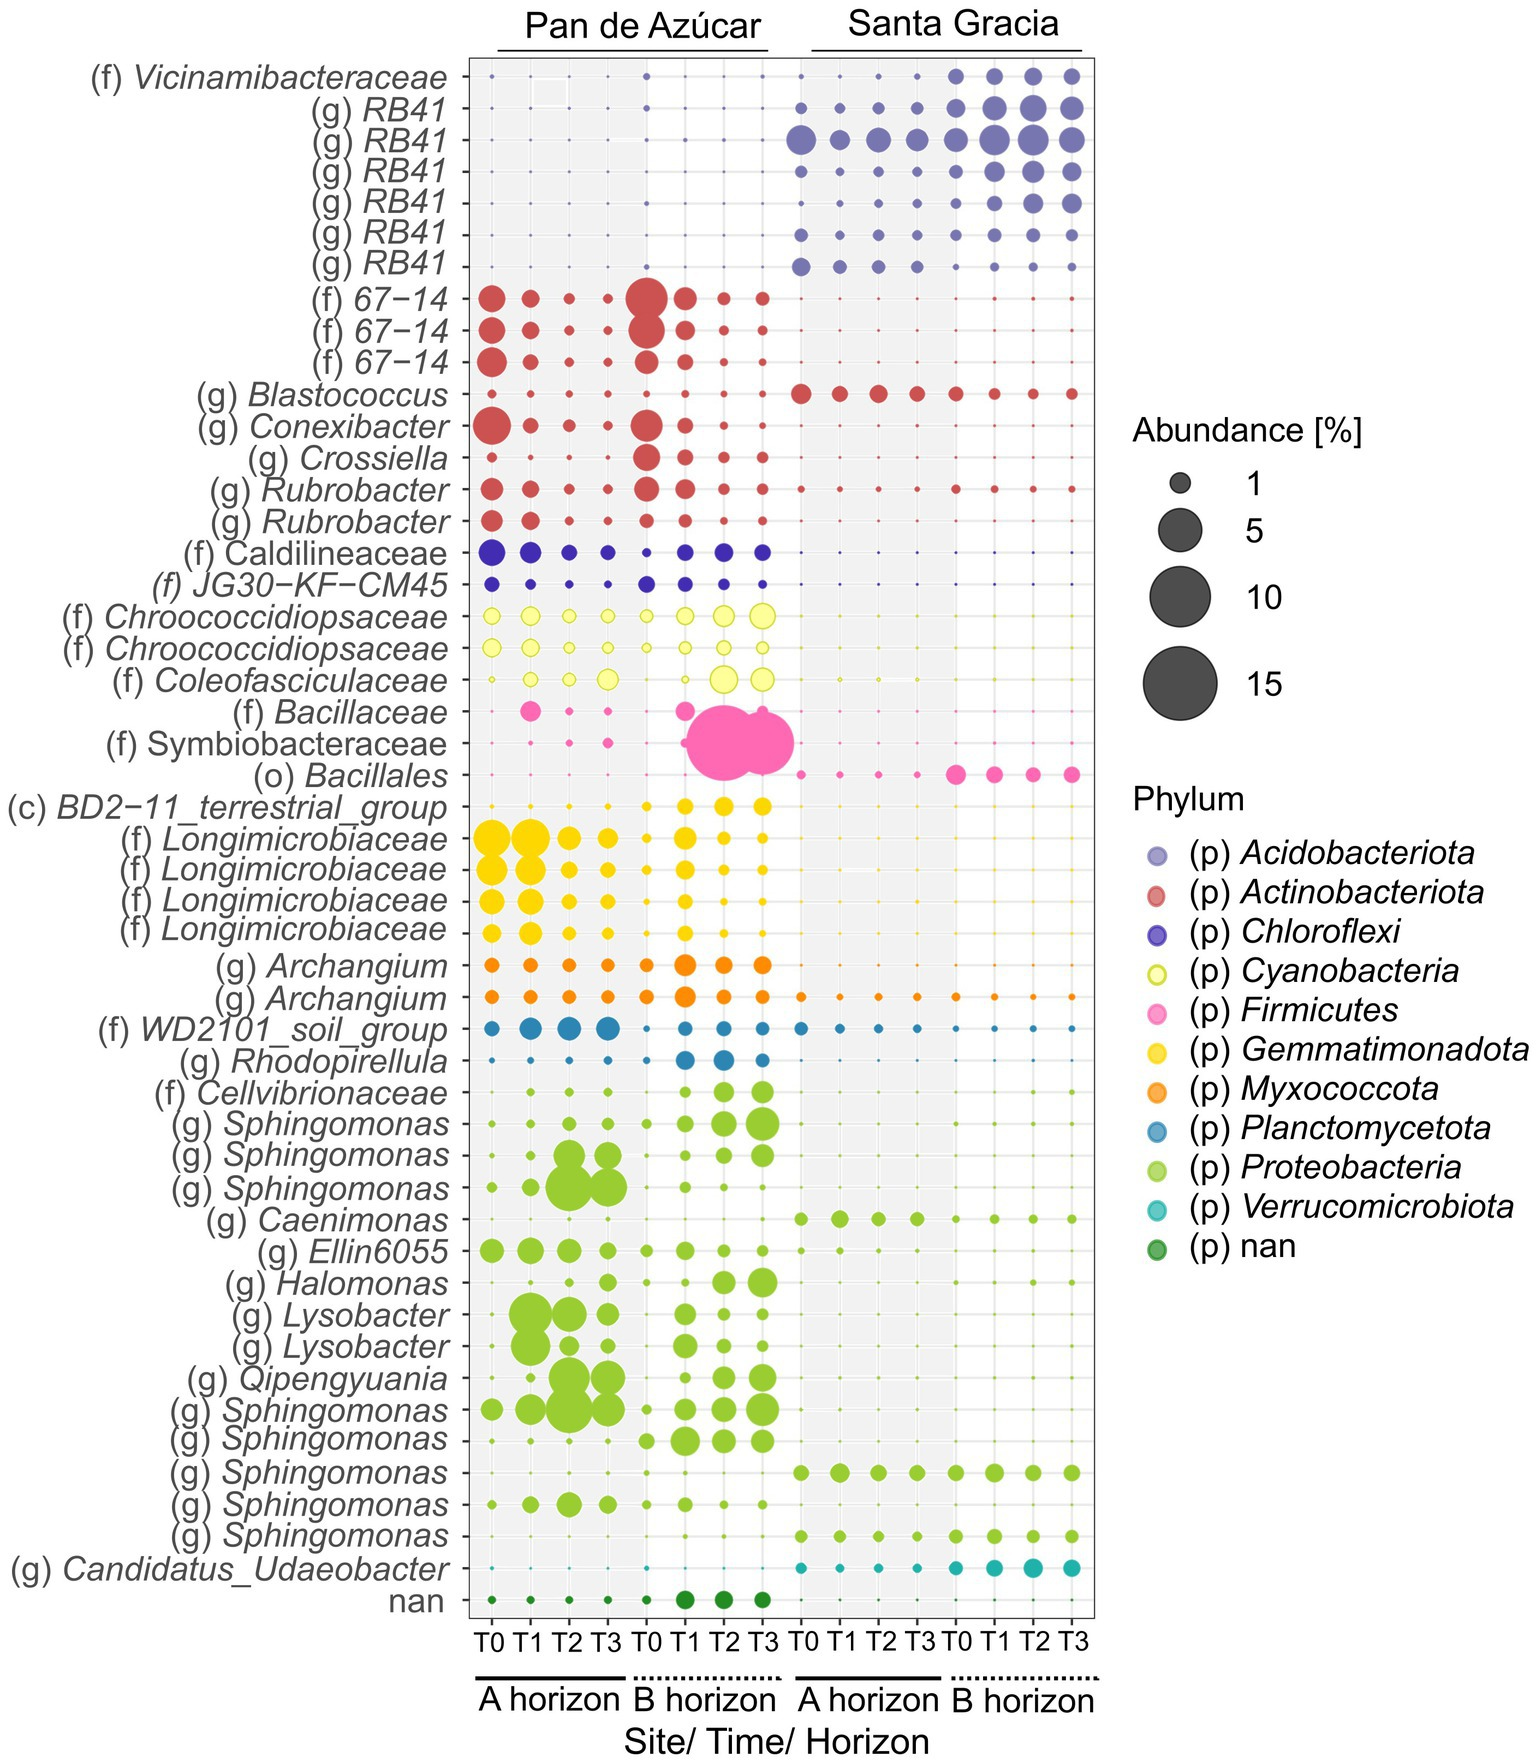
\includegraphics[width=1\textwidth]{img/M3-Figure_6.jpg}
	\caption[Top 50 relative abundance of indicator species for Pan de Azúcar and Santa Gracia in four time points of the soil manipulation experiment]{Top 50 relative abundance of indicator species for Pan de Azúcar and Santa Gracia in four time points of the soil manipulation experiment. Colors represented different phyla. Time is represented as T0 (original), T1 (2 weeks), T2 (12 weeks), and T3 (16 weeks). Each bubble is the mean of the different treatments (in situ, BSCs, and plants) and biological triplicates. Taxa are shown on the level of class (c), order (o), family (f), and genus (g).}
	\label{fig:M3-F6}
\end{figure}

\subsection{Co-occurrence network}

We employed a co-occurrence network to explore the dynamics and relationships within bacterial communities across both sites (PA and SG) sharing the same parent material. 
Among the \num{280} ASVs analyzed, we identified seven modules of highly correlated ASVs represented by different colors (\ref{fig:M3-F7}). 
Based on their correlation patterns, these modules formed two sub-networks: Subnetwork 1 consisted of the brown and turquoise modules, while Subnetwork 2 comprised the green, red, yellow, black, and blue modules. 
Notably, the ASVs within the subnetworks showed different preferences for specific sites. 

\begin{figure}[H]
	\centering
	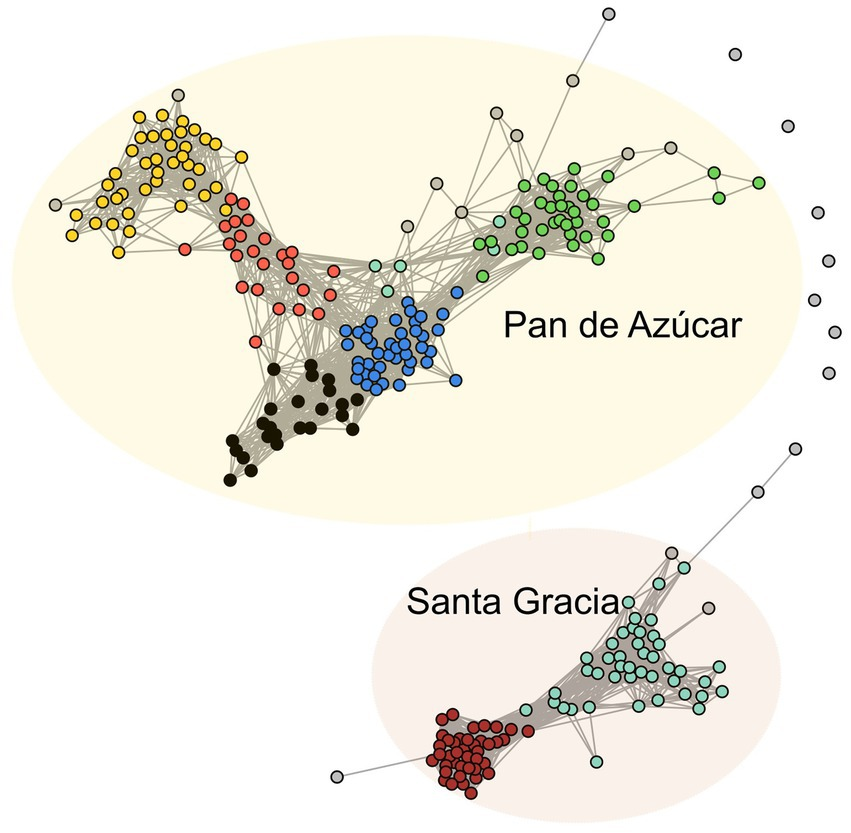
\includegraphics[width=1\textwidth]{img/M3-Figure_7.jpg}
	\caption[Co-occurrence network of bacterial ASVs]{Co-occurrence network of bacterial ASVs. The nodes (ASVs) in the network are colored by modularity. The connections stand for a strong (R > 0.7) and significant (p < 0.01) correlation. The network was subdivided into two subnetworks corresponding to Pan de Azúcar and Santa Gracia.}
	\label{fig:M3-F7}
\end{figure}

\begin{table}[ht]
	\centering
	\caption[Co-occurrence network topological metrics]{Co-occurrence network topological metrics.}
	\label{tab:M3-T1}
	\begin{tabular}{lcc}
	\hline
	\textbf{Network metrics} & \textbf{Pan de Azúcar} & \textbf{Santa Gracia} \\
	\hline
	No. of nodes\textsuperscript{1} & 185 & 88 \\
	No. of edges\textsuperscript{2} & 2,054 & 1,149 \\
	Average degree\textsuperscript{3} & 11.1 & 13.02 \\
	Cluster coefficient\textsuperscript{4} & 0.639 & 0.798 \\
	Modularity\textsuperscript{5} & 0.589 & 0.429 \\
	Connectance\textsuperscript{6} & 0.060 & 0.148 \\
	\hline
	\end{tabular}
	
	\vspace{0.5em}
	\begin{minipage}{0.9\textwidth}
	\footnotesize
	\textsuperscript{1}Number of ASVs with at least one correlation.\\
	\textsuperscript{2}Number of strong and significant correlations between nodes.\\
	\textsuperscript{3}How many connections on average each node has to another unique node in the network.\\
	\textsuperscript{4}Degree to which nodes tend to cluster together.\\
	\textsuperscript{5}Indicate the partition in modules.\\
	\textsuperscript{6}Ratio between the number of realized edges and the number of potential edges within the network \citep{DiniAndreote2014, Karimi2017}.
	\end{minipage}
	\end{table}
	
	

Subnetwork 1 was predominantly found in SG, whereas Subnetwork 2 was more abundant in PA. In subnetwork 1 (SG), Acidobacteriota (34), Proteobacteria (21), and Verrucomicrobiota (14) accounted for \SI{78.4}{\percent} of the total ASVs. In subnetwork 2 (PA), the most abundant taxa were Proteobacteria (47), Actinobacteriota (23), and Gemmatimonadota (21), representing \SI{49}{\percent} of total ASVs.

We proceeded to analyze the topological properties of each subnetwork to understand the interrelationship patterns between nodes, as summarized in \ref{tab:M3-T1}. Initially, the network consisted of 273 nodes (ASVs) and \num{3203} edges (correlations). After subdivision, the subnetwork 2 (PA) exhibited more nodes and edges, accounting for \SI{66}{\percent} of all ASVs. Subnetwork 1 (SG) displayed a higher average degree (node connectivity degree), connectance, and clustering coefficient (degree of nodes tended to cluster together), indicating highly connected and densely clustered modules. On the other hand, subnetwork 2 (PA) showed higher modularity (degree of division into modules), indicating a clear division into modules. Additionally, we observed that the abundance patterns of ASVs within the modules varied depending on the horizon. In PA, the green and blue modules were more abundant in the A horizon, while the yellow and red modules were more abundant in the B horizon. In SG, the ASVs of the brown module were more abundant in the B horizon, while the turquoise module exhibited a slightly higher abundance in the A horizon.

We identified the top hub ASVs per module to gain further insights into the highly connected species within the co-occurrence networks. The hub ASVs in SG belonged to the family Comamonadaceae in the turquoise module and the genus \textit{Candidatus Udaeobacter} in the brown module. On the other hand, in PA, hub ASVs were identified from the family Sphingobacteriaceae (green), Longimicrobiaceae (blue), 67–14 (black), Ardenticatenaceae (red), and WD2101 soil group (yellow).

We utilized the identified modules to correlate them with physicochemical properties and examine their associations (\ref{fig:M3-F8}). The modules representing SG displayed a distinct pattern based on organic matter content. The turquoise module positively correlated with TOC, N\textsubscript{bulk}, and N\textsubscript{t} in different aggregate sizes (\(R > 0.8\)). Conversely, the turquoise and brown modules negatively correlated with pH (\(R < -0.7\)). In PA, the black module demonstrated a strong positive correlation with sodium and chloride, while the blue module was correlated with pH (\(R=0.7\)). The red module displayed associations with C\textsubscript{t} content in macroaggregates, sodium, potassium, sulfate, pH, and EC (\(R > 0.7\)). Additionally, the yellow module exhibited a strong positive correlation with C\textsubscript{t} in microaggregates, sulfate, and EC (\(R > 0.7\)).

\begin{figure}[H]
	\centering
	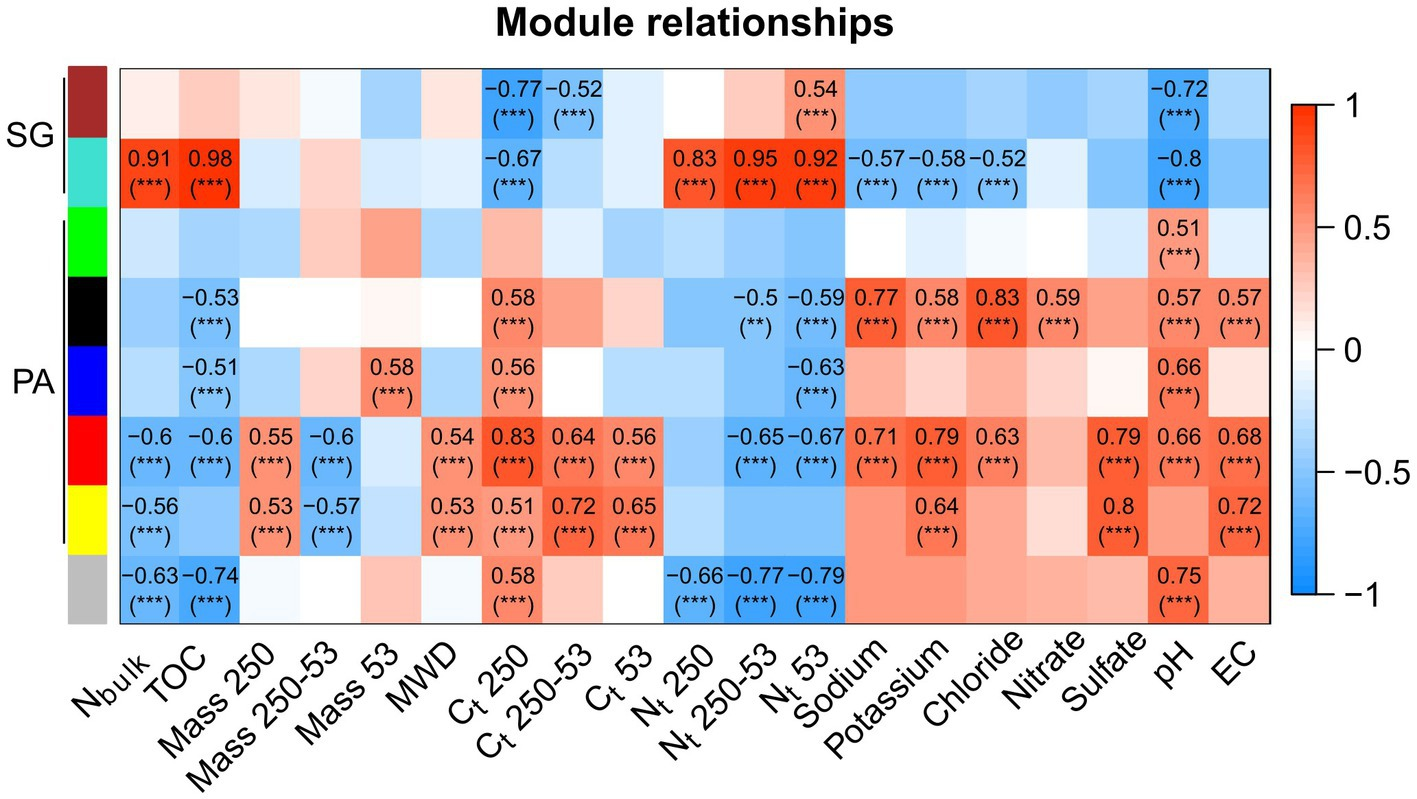
\includegraphics[width=1\textwidth]{img/M3-Figure_8.jpg}
	\caption[Pearson correlation of modules from the co-occurrence network and soil physicochemical properties in Pan de Azúcar and Santa Gracia]{Pearson correlation of modules from the co-occurrence network and soil physicochemical properties in Pan de Azúcar (PA) and Santa Gracia (SG). Only correlations greater than $R = 0.5$ are shown. Significance levels are indicated as follows: ``\textbf{**}'' for $p < 0.01$ and ``\textbf{***}'' for $p < 0.001$.
	The physicochemical properties included nitrogen in the bulk soil (N\textsubscript{bulk}), total organic carbon (TOC), total mass in macroaggregates (Mass 250), total mass in large microaggregates (Mass 250--53), total mass in small microaggregates (Mass 53), mean weight diameter (MWD), total carbon in macroaggregates (Ct 250), total carbon in large microaggregates (Ct 250--53), total carbon in small microaggregates (Ct 53), nitrogen in macroaggregates (Nt 250), nitrogen in large microaggregates (Nt 250--53), nitrogen in small microaggregates (Nt 53), sodium, potassium, chloride, nitrate, sulfate, pH, and electrical conductivity (EC).
	}
	\label{fig:M3-F8}
\end{figure}

\section{Discussion}

This study investigated the interplay between biotic and abiotic factors during soil formation within initial arid and semiarid soils under simulated climate change (humid climate conditions). We focused on exploring the direct impact of microbial communities on the early stages of soil formation and their interactions with BSCs and plants by analyzing changes in soil physicochemical properties along the different treatments. Further, we examined the bacterial community response of arid and semiarid soils to simulated climate change to gain insights into their potential adaption to the changed conditions.

\subsection{Abiotic versus biotic influence on soil formation in arid and semiarid soils under climate change}

A simulated humid climate that mimicked a climate change scenario along the Chilean Coastal Cordillera stimulated the initial soil formation in all treatments. The extent of this ``climate change'' effect on soil formation varied by soil origin and horizon but did not differ from the sterile treatment. This indicates that the abiotic influence on initial soil formation was larger than the biotic influence over the short simulation period. The formation of macroaggregates, the loss of large microaggregates, and the associated increase in MWD in the B horizon of PA were likely influenced by elevated levels of carbonates (e.g., \ce{CaCO3}). The prevalence of inorganic carbon in the form of carbonates is supported by the high C\textsubscript{t} values coupled with low TOC concentrations, as corroborated by prior studies \citep{SchulzeMakuch2018, RiverasMunoz2022}. Water likely facilitated the diffusion of cations, stimulating carbonate precipitation to form secondary carbonate coatings and bind primary soil particles, thus enhancing soil structure \citep{Bronick2005}. Additionally, notable reductions in EC in the A horizon of PA and sodium and chloride concentrations in the B horizon of PA were observed, likely due to the leaching of exchangeable base cations and soluble salts as reported by \citet{Bernhard2018}, consistent with previous findings in saline-alkali soils \citep{Wang2017}. Lastly, the increase in TOC in the B horizon of SG compared to the A horizon indicates a contrasting response in carbon mobility and retention between the two horizons, potentially driven by enhanced mineral adsorption capacity or increased occlusion of organic matter into aggregates \citep{Kramer2018}. These findings highlight the influence of soil origin (site and horizon) and their physicochemical properties on the response to climate change over time.

The microorganisms-plant treatment positively influences arid and semiarid soil stabilization, indicated by increased macroaggregate formation and MWD in SG and the A horizon of PA at 16 weeks relative to the other treatments. In contrast, this beneficial effect was not observed in the B horizon of PA, due to poor root development and premature plant mortality promoted by high salinity and nutrient deficiency during the manipulation experiment. The observed effect can be attributed to the enmeshment and realignment of soil particles by roots and the release of exudates, leading to significant physical, chemical, and biological alterations that influence soil aggregation \citep{Bronick2005}. Prior studies support the role of fine sand and fine roots as co-drivers of aggregate stability in early successional stages of mediterranean soils \citep{Erktan2016} and the promotion of macroaggregate formation through root exudates favoring fungi in carbon-poor forest subsoils \citep{Baumert2018}. Additionally, field experiments have shown that water addition in the presence of plants enhances macroaggregation, probably due to increased root activity, fungal enmeshment, and microbial access to carbon substrates for exopolysaccharide production \citep{Blankinship2016}. While converting desert soil into irrigated cropland with profitable harvest typically requires at least 50 years \citep{Su2010}, and natural soil development processes occur over much longer timescales spanning hundreds to thousands of years \citep{Jenny1994}, our findings reveal the early measurable impact of microorganisms-plant associations on the soil stabilization even in short-time scales of weeks.

Microorganisms alone and in conjunction with BSCs had no discernible impact on the measured physicochemical parameters compared to sterile soils under the experimental settings. The absence of changes can be attributed to the potentially more prominent influence of water, which likely overshadowed the effects of microorganisms, resulting in a water-masking effect. This finding aligns with a previous six-month manipulation experiment on mediterranean soil, highlighting the increased significance of microorganisms in aggregation under drier conditions, where limited water availability restricts abiotic macroaggregate formation but supports active microbial communities \citep{Blankinship2016}. Similarly, a field study proposed that plants and organic matter exert a stronger influence on aggregation than BSCs in wetter conditions along a climate gradient, while BSCs are significant compared to bare soil, including microorganisms in drier environments \citep{RiverasMunoz2022}. Moreover, a previous study in SG reported no significant increase in N-fixation and even a decrease in nitrogen mineralization in SG when soil moisture reached \SI{57}{\percent} of water-filled pore space \citep{Seuss2022}. Based on these findings, our results suggest that the applied water content (\SI{65}{\percent} water-filled pore space) may exceed the threshold required to activate specific biogeochemical processes facilitated by microorganisms. Alternatively, it is plausible that soil properties like organic carbon and acidity exhibit slower changes than the microbial community structure alone, considering their short generation times, allowing them to adapt and respond rapidly to environmental changes \citep{Placella2012}.

On the other hand, our study may have overlooked the initial effects of microorganisms on soil properties when analyzing bulk soil samples taken across an entire soil horizon. This limitation could also dilute the impact of BSCs, which primarily influence the soil properties near the surface, progressively decreasing with depth \citep{Miralles2020}. Microorganisms might influence soil properties at a smaller spatial scale beyond the resolution of our bulk soil analyses. For instance, nanoscale secondary ion mass spectrometry analysis in vertisol and alfisol soils demonstrated the crucial role of microbially metabolized nitrogen in promoting organo-mineral associations, impacting organic matter cycling, immobilization, and storage \citep{Kopittke2018}. However, despite the lack of independent impact detected, microorganisms likely played an important role in improving soil conditions by mitigating abiotic stress factors, such as high pH, salinity, and nutrient limitations for plant-microorganism treatment \citep{Etesami2017}. This beneficial effect is exemplified by the active recruitment of growth-promoting bacteria, including N-fixing bacteria, by plant roots in the Atacama desert \citep{Eshel2021}, which may have influenced the observed differentiation of bacterial communities among treatments by the end of the soil manipulation experiment.

\subsection{Bacterial communities inhabiting arid and semiarid soils respond differently to climate change}

Differential responses of bacterial communities were observed at the two different sites under simulated climate change. Notably, bacterial communities increased in gene copy numbers in PA, the arid site (in contrast to SG, the semiarid site), revealing higher bacterial activity or growth based on higher cellular ribosome contents \citep{Placella2012}. This increase in gene copy numbers can be attributed to the ``Birch effect,'' which is influenced by wetting and promotes the breakdown of aggregates, mineralization of dead microbial cells and osmolytes, and subsequent release of nutrients such as carbon \citep{Jarvis2007}. This phenomenon has been observed in arid and semiarid soils \citep{Armstrong2016, Seuss2022}, where releasing organic compounds potentially enhances bacterial reproduction and growth. This finding could explain the correlation between the bacterial community and nitrogen content in the A horizon of PA after two weeks of the soil manipulation experiment or the enhanced predicted functions related to chemoheterotrophy and organic matter degradation processes. These results evidence alterations in substrate availability and concomitant growth dynamics, which can be linked to the initial activation of soils triggered by nutrient inputs in the system promoted by humid climate conditions \citep{Nemergut2016, ChenLeung2021}.

Contrasting the gene copy numbers, changes in diversity indices over time reveal a decrease in the Shannon index in PA while remaining stable in SG. This is attributed to the degree of bacterial specialization, which is different in both sites. PA exhibits a high degree of bacterial specialization as an evolutionary response to a stable environment in time and space \citep{Rodriguez2022}, while sudden climate shifts can act as stressors that promote a reduction in diversity \citep{Clavel2011}. In contrast, SG represents a heterogeneous and disturbed ecosystem dominated by bacterial generalists \citep{Rodriguez2022}, benefiting from their metabolic flexibility to thrive in highly dynamic environments \citep{Hawkes2020, ChenNeilson2021}. Our findings follow a previous study demonstrating that frequent drying-wetting stress may favor tolerant microbial taxa in SG \citep{Seuss2022}. This also can be illustrated by other studies where in the hyperarid Atacama Desert, diversity decreases when water is rapidly and abundantly applied \citep{AzuaBustos2018}, while a desert steppe with mean annual precipitation of \SI{289}{\milli\metre} showed no response to altered precipitation regimes \citep{Na2019}. Furthermore, \citet{StovicekB2017} found higher diversity in deserts due to disconnected soil niches, but wetter soil conditions reduce diversity through dispersion, connectivity, homogenization, and nutrient fluxes. Given the association between bacterial diversity and enzymatic activities related to nitrogen and phosphorus cycles, as well as plant productivity \citep{DelgadoBaquerizo2016, Luo2018}, the decrease of diversity in PA could negatively affect soil formation due to a smaller number of available metabolic pathways \citep{Shen2023}.

The degree of bacterial specialization is reflected in the shift of taxonomic composition observed at different sites. PA exhibits an early community reassembly from phyla to the ASV level, along with variations in indicator species, indicating a different tolerance threshold compared to SG. In the A horizon of SG, the dominant phyla and indicator species remained steady, but a change occurred at the ASV level after 16 weeks, while the B horizon maintained ASV stability from 2 to 16 weeks. These findings can potentially be attributed to two microbial adaptation strategies \citep{Uritskiy2019}: In PA, new bacteria from the seed bank come in through niche intrusion, while SG adjusts its existing fitness-based community structure to withstand new selective pressures and prevents the dominance of new bacteria. A study on grasslands assessing drought and precipitation extremes based on mean annual precipitation revealed an unchanged soil bacterial composition, suggesting a high level of community and functional resistance in areas with climate variability \citep{Hawkes2020}. Conversely, studies in the Namib and Negev deserts demonstrate changes in bacterial composition following precipitation events \citep{Armstrong2016, StovicekA2017, Ouyang2020}, supporting the notion that more arid ecosystems are more susceptible to precipitation impacts.

The succession dynamic in PA is evident through the shift in taxonomic composition, initially dominated by Actinobacteriota and gradually replaced by Proteobacteria. Actinobacteriota thrive in oligotrophic environments, particularly during early soil succession, and can affect the soil organic matter formation and biogeochemical cycles \citep{Zhang2019, Yu2022}. However, their abundance decreases with increasing water availability as the corresponding species are adapted to dry conditions \citep{Barnard2013, Maestre2015, StovicekA2017}. This shift is exemplified by the reduction in desiccation-resistant species like \textit{Rubrobacter} or Solirubrobacterales (\textit{Conexibacter} and 67–14), which include genes for chemosynthetic \ce{CO2} fixation \citep{SchulzeMakuch2018, Meier2019}. Similarly, Gemmatimonadota, known for its potential roles in carbon fixation and \ce{N2O} reduction and adapted to extreme environments such as saline soils, also showed a decreasing abundance with increased water content \citep{Mujakic2022}. Notably, the Longimicrobiaceae family within this phylum, which could facilitate phosphate solubilization in the soil, showed a marked decline \citep{Korkar2022}. In contrast, while Cyanobacteria overall declined, the Chroococcidiopsaceae genus, a potential primary producer in the Atacama Desert using nitrate and ammonium, remains stable \citep{SchulzeMakuch2021}. Our study aligns with previous research showing the potential ability of PA bacterial communities to fix and accumulate organic matter \citep{Rodriguez2022}, highlighting the potential negative consequences of diminishing these bacterial taxa on soil fertility.

Increased water availability, the release of organic compounds, and the accumulation of elements via long-term weathering and climate processes can create a relatively nutrient-rich habitat, favoring copiotroph groups such as Bacteroidota (correlated with nitrogen and TOC) and Proteobacteria (correlated with chemoheterotrophy) in PA \citep{Na2019, Zhao2019}. Among these, Proteobacteria are widely distributed and preferentially use the labile pool of organic carbon \citep{Fierer2007}. They exhibit metabolic versatility, encompassing functional groups such as phototrophs, chemoorganotrophs, and chemolithotrophs \citep{Kersters2006}, allowing them to utilize multiple energy sources, carbon substrates, and electron acceptors \citep{ChenNeilson2021}. From this phylum, functions such as microaggregate formation through the excretion of extracellular polymeric substances have been associated with the genus \textit{Sphingomonas} and also with the family Sphingobacteraceae (Bacteroidota), which include several indicators and one hub species \citep{CaesarTonthat2007, Pankratov2007, Vuko2020}. Remarkably, their abundance increased over time, potentially influencing the stabilization of soil aggregates and the increased MWD in our manipulation experiment. While the new community displays increased versatility and potential new functions, it is crucial to recognize that the loss of taxa could disrupt soil ecosystem processes, functions, and stability \citep{Bestion2020}.

Proteobacteria, Acidobacteriota, and Planctomycetota steadily dominated the A horizon of SG and the B horizon of SG at 16 weeks. This finding is consistent with previous studies reporting a prevalence of these phyla during the successional development of tundra soils, the desert, and after deglaciation \citep{Zhelezova2019, Yu2022, Shen2023}. Acidobacteriota, known as heterotrophic-oligotrophs, are well-adapted to harsh environmental conditions with limited carbon availability \citep{Fierer2007, Zhao2019}. Genomic analysis of Acidobacteriota has revealed their metabolic flexibility and versatility, with the potential capacity to participate in sulfur metabolism and utilize diverse carbohydrates, as is also indicated by the indicator species RB41 \citep{Eichorst2018, Kalam2020, Stone2021}. Furthermore, Acidobacteriota has numerous genes related to the nitrogen cycle \citep{Eichorst2018}, highlighting their potential role in nitrogen dynamics, further supported by its correlation with N\textsubscript{t}. On the other hand, Planctomycetota exhibits both copiotrophic and oligotrophic features, adapting to varying carbon availability \citep{Lauro2009}. The metabolic versatility of these dominant phyla positions them as potential players in organic matter balance and ecological dynamics.

Our co-occurrence network analysis confirms the distinction between the soil environments of PA and SG. Specifically, the SG subnetwork demonstrates greater complexity than PA, as indicated by a higher average degree, connectance, and lower modularity \citep{Karimi2017, Tu2020}. This finding is in agreement with previous research that has reported a higher average degree in more advanced successional stages within an early chronosequence \citep{Sun2017}, in conjunction with increased nutrient availability \citep{Zhao2019} and with higher diversity \citep{Tu2020}, as found in SG. Furthermore, our findings indicate a higher resilience to environmental perturbations in SG, consistent with previous studies associating higher connectance and complexity to functional redundancy of interactions \citep{Tylianakis2010, Karimi2017, Wu2021}. On the other hand, the PA subnetwork displayed a more modular structure, indicating that bacterial communities within the same module share a similar ecological niche \citep{Tu2020}. These niches are shaped by nutritional preferences, functional distinctiveness, and interaction with physicochemical properties \citep{Banerjee2016}. Specifically, the red and yellow modules, mainly composed of Proteobacteria, showed associations with C\textsubscript{t} in macro- and large microaggregates and EC, suggesting their involvement in carbon sequestration as carbonates in saline-alkali soils \citep{Qu2022}. This, in turn, could link the carbonate content and MWD in these modules. Additionally, the yellow module, positively correlated with sulfate, contained the species MW2101 (phylum Planctomycetota), among others encoding proteins similar to sulfatases, potentially enabling efficient access to the carbon of sulfated compounds as energy and carbon sources \citep{Dedysh2021}. In SG, the turquoise module positively correlated with nitrogen, which could be related to the high number of Acidobacteriota and the N-fixing family Comamonadaceae in this module \citep{Eichorst2018, Vuko2020}. Our results highlight the importance of bacterial clustering within specific modules, providing information about niche partitioning, synergistic relationships, and overall soil functioning \citep{DiniAndreote2014}.

\subsection{Soil and climate legacy play a role in shaping the response of initial soil formation and bacterial communities to climate change}

Under the simulated climate change scenario, the arid soil of PA exhibited a more pronounced response compared to the semiarid soil of SG. The greater shifts in physicochemical properties and soil bacterial communities in arid soils under climate change are attributed to the influence of climate legacies, which have emerged as key drivers shaping the response of bacterial communities to climate disturbances \citep{DelgadoBaquerizo2017a, DelgadoBaquerizo2018}. Evidence from cosmogenic nuclide analysis supports the existence of a stable and hyperarid climate in PA throughout the Pliocene and Pleistocene \citep{Placzek2009}. Even other studies indicated climate stability from the late Jurassic, as inferred from paleomagnetic data \citep{Hartley2005}. In contrast, the region between \ang{30} to \ang{35} S with the study site SG has experienced significant influences from glacial advances, periglacial effects, and climatic changes \citep{Arroyo2012}. The differences between both sites and our findings indicate that SG harbors a more tolerant bacterial community, enabling them to adopt different functional repertoire modes, compete for resources, and maintain taxonomic stability even under changing environmental conditions. In contrast, being sensitive and reactive, the bacterial community in PA has changed toward a more versatile community with potentially new functions, as can be inferred from the new taxa in response to the humid climate of Nahuelbuta that has been applied experimentally to mimic climate change. However, this bacterial replacement, associated with vulnerability to disturbances, can impact the ability of the community to self-sustain its functioning and ecosystem stability \citep{ChenLeung2021}. Therefore, it is necessary to investigate whether taxonomic changes are linked to functional changes using additional tools such as metagenomics and metatranscriptomics to gain insights into the potential roles of bacteria in the initial soil transformation.

We further propose that soil and climate legacy is important not only for the soil bacterial community and its response but also for future soil development under climate change. Soil and climate legacies, which can be understood as the resilience of the system, have influenced less soil development in PA (as indicated by high pH and salinity values (EC) and low TOC, nitrogen, bacterial abundance, and plant development). In contrast, SG has shown a progressive soil formation with organic matter accumulation, increased vegetation cover (\SIrange{30}{40}{\percent} shrubs and cacti), and a pH decrease due to increased precipitation and reduced temperature from PA to SG \citep{Bernhard2018}. This presumably promoted different short-term trajectories of soil formation between sites and horizons, impacting the decomposition rate of organic matter, mineral leaching, and plant development differently. Previous studies support our findings by studying the legacy effects of climate and soil moisture on carbon stocks, nutrients, plant growth, and mycorrhizal responsiveness \citep{Cavagnaro2016, DelgadoBaquerizo2017b}. In turn, the legacy of resource availability modulates microbial resource responses \citep{Yuan2022}. Therefore, the soil and climatic legacy shapes soil formation by influencing microbial communities, physicochemical properties, biogeochemical cycles, nutrient availability, and carbon dynamics, providing crucial insights for managing soil sustainability in different soil environments.

\section{Conclusion}

Soil formation is crucial for life on Earth and biogeochemical cycles; therefore, understanding the role of microorganisms in this process is vital for gaining insights into ecosystem dynamics. Our findings demonstrate that microorganism-plant interaction drives short-term soil development and stabilization in arid soils exposed to humid climate conditions, even on short time scales of weeks. Interestingly, microorganisms alone and in conjunction with BSCs did not play a measurable role in soil formation under the same conditions. Hence, the microorganism-plant interaction has a faster and more robust impact on altering soil physicochemical properties in humid climate conditions than microorganisms alone. Furthermore, we identified a distinct sensitive and specialized bacterial community in arid soil, contrasting with the more complex, versatile, and stable bacterial community observed in semiarid soil, which we attribute to climate legacies. Our findings are relevant to understanding the intricate dynamics and complexity of bio-geo interactions between biota and climate on soil formation, providing insights into soil management (e.g., efficient irrigation), long-term ecosystem sustainability in arid regions, and the bacterial response to climate change.

\section*{Data availability statement}

The datasets presented in this study can be found in online repositories. The names of the repository/repositories and accession number(s) can be found below: 

EBI - \url{https://www.ebi.ac.uk/ena/browser/view/PRJEB60029}

\section*{Author contributions}

VR: Formal analysis, Investigation, Methodology, Visualization, Writing - original draft, Writing - review \& editing. AB: Data curation, Formal analysis, Methodology, Supervision, Writing - review & editing. KW: Formal analysis, Methodology, Writing - review \& editing. NR-M: Formal analysis, Methodology, Writing - review \& editing. RO: Conceptualization, Supervision, Writing - review \& editing. SL: Supervision, Writing - original draft, Writing - review \& editing. JK: Formal analysis, Methodology, Writing - review \& editing. OR: Formal analysis, Methodology, Writing - review \& editing. CM: Conceptualization, Writing - review \& editing. OS: Conceptualization, Writing - review \& editing. TS: Conceptualization, Writing - review \& editing. DW: Conceptualization, Supervision, Writing - original draft, Writing - review \& editing.

\section*{Funding}

The author(s) declare financial support was received for the research, authorship, and/or publication of this article. This research was supported by the BECAS Chile 2019 program via a grant to VR (72200201) and by the Deutsche Forschungsgemeinschaft (DFG) in the framework of the priority program “EarthShape—Earth Surface Shaping by Biota (SPP 1803)” by a grant to TS (SCHO 739/17) and CM (MU 3021/6-2). The 16S rRNA gene amplicon sequencing done in Wagner's lab was financed through the Helmholtz Research Program “Changing Earth - Sustaining our Future.”

\section*{Acknowledgments}

The authors wish to thank the Chilean National Park Service (CONAF) and Sucesión Gálvez Muñoz, who provided access to the study sites. The authors also wish to express our deep gratitude to all the colleagues who helped in the field and with logistics during the several months of field work—especially Kirstin Übernickel (University of Tübingen) and Leandro Paulino (Universidad de Concepción).

\section*{Conflict of interest}

The authors declare that the research was conducted in the absence of any commercial or financial relationships that could be construed as a potential conflict of interest. The author(s) declared that they were an editorial board member of Frontiers, at the time of submission. This had no impact on the peer review process and the final decision.

\section*{Publisher's note}

All claims expressed in this article are solely those of the authors and do not necessarily represent those of their affiliated organizations, or those of the publisher, the editors and the reviewers. Any product that may be evaluated in this article, or claim that may be made by its manufacturer, is not guaranteed or endorsed by the publisher.

\section*{Supplementary material}

The Supplementary material for this article can be found online at: 
\url{https://www.frontiersin.org/articles/10.3389/fmicb.2024.1319997/full#supplementary-material}

\chapter{Microbially induced soil aggregate turnover across different climates and moisture regimes}
\label{chap:manuscript4} % Label for potential cross-referencing (start page)
\chapter{Living and decaying roots as regulators of soil aggregation and organic matter formation---from the rhizosphere to the detritusphere}
\label{chap:manuscript5} % Label for potential cross-referencing (start page)

\begin{center}
    \textbf{\Large Manuscript 5}
  
    \vspace{0.3cm}
    \textit{Soil Biology and Biochemistry}\\
    \textit{DOI 10.1016/j.soilbio.2024.109503}
    
    \vspace{0.5cm}
    \begin{justify}
    Kristina Witzgall\textsuperscript{1}, Franziska Steiner\textsuperscript{1}, Benjamin D. Hesse\textsuperscript{2,3}, Nicolás Riveras-Muñoz\textsuperscript{4}, Victoria Rodríguez\textsuperscript{5}, Pedro Teixeira\textsuperscript{1}, Li, M.\textsuperscript{6}, Rómulo Oses\textsuperscript{7}, Oscar Seguel\textsuperscript{8}, Steffen Seitz\textsuperscript{4}, Dirk Wagner\textsuperscript{5,6}, Thomas Scholten\textsuperscript{4}, Franz Buegger\textsuperscript{9} Gerrit Angst\textsuperscript{7,11,12}, and Carsten W. Mueller\textsuperscript{1,13,14}
    \end{justify}
    \vspace{0.2cm}
  \end{center}
  
  \begin{scriptsize}
    \begin{justify}
        \textsuperscript{1}Soil Science, TUM School of Life Sciences, Technical University of Munich, Freising-Weihenstephan, Germany\\
        \textsuperscript{2}Land Surface Atmosphere Interactions -- AG Ecophysiology of Plants, TUM School of Life Sciences, Technical University of Munich, Freising-Weihenstephan, Germany\\
        \textsuperscript{3}Institute of Botany, Department of Integrative Biology and Biodiversity Research, University of Natural Resources and Life Sciences, Vienna, Austria\\
        \textsuperscript{4}Department of Geosciences, Soil Science and Geomorphology, University of T\"ubingen, T\"ubingen, Germany\\
        \textsuperscript{5}GFZ German Research Centre for Geosciences, Section Geomicrobiology, Potsdam, Germany\\
        \textsuperscript{6}Institute of Geosciences, University of Potsdam, Potsdam, Germany\\
        \textsuperscript{7}Biology Centre of the Czech Academy of Sciences, Institute of Soil Biology \& SoWa Research Infrastructure, \v{C}esk\'{e} Bud\v{e}jovice, Czech Republic\\
        \textsuperscript{8}Centro Regional de Investigaci\'{o}n y Desarrollo Sustentable de Atacama (CRIDESAT), Universidad de Atacama, Copiap\'{o}, Chile\\
        \textsuperscript{9}Facultad de Ciencias Agron\'{o}micas, Universidad de Chile, Santiago, Chile\\
        \textsuperscript{10}Research Unit Environmental Simulation, Helmholtz Zentrum M\"unchen (GmbH), German Research Center for Environmental Health, Neuherberg, Germany\\
        \textsuperscript{11}German Centre for Integrative Biodiversity Research Halle--Jena--Leipzig (iDiv), Leipzig, Germany\\
        \textsuperscript{12}Institute of Biology, Leipzig University, Leipzig, Germany\\
        \textsuperscript{13}Institute for Ecology, Chair of Soil Science, Technische Universit\"at Berlin, Berlin, Germany\\
        \textsuperscript{14}Department of Geosciences and Natural Resource Management, University of Copenhagen, Copenhagen, Denmark
    \end{justify}
  \end{scriptsize}
    
  \vspace{0.5cm}
  \begin{center}
    Received: 27 February 2024\\
    Received: 13 November 2023\\ 
    Received in revised form: 15 June 2024\\
    Accepted: 17 June 2024\\
    Available online: 18 June 2024
  \end{center}
  \cleardoublepage

\section*{Abstract}

In dryland ecosystems, typically characterized by sparse vegetation and nutrient scarcity, pioneer plants exert a critical role in the build-up of soil carbon (C). Continuous root-derived C inputs, including rhizodeposition and structural root litter, create hotspots of increased microbial activity and nutrient availability where biogeochemical processes, such as soil aggregation and the accumulation and stabilization of organic matter (OM), are promoted. Our study aims to disentangle the effects of root C inputs on soil aggregate formation, microbial community structures, and on the fate of OM—both before and after plant death, i.e., during the transition from rhizosphere to detritusphere. This was realized in a two-phase incubation approach, tracing the natural and undisturbed transition from growth to subsequent decomposition of a pioneer plant-root system (\textit{Helenium aromaticum}) in a semi-arid topsoil and subsoil. We quantified water-stable aggregates, investigated the fate and composition of OM separated into particulate and mineral-associated OM fractions (POM and MAOM), and observed successional changes in the root-associated microbiome. Our results underscore the significance of roots as vectors for macroaggregation within the rhizosphere in both topsoil and subsoil, associated with a particularly strong increase in fungal abundance in the subsoil. In topsoil, we identified root legacy effects in the detritusphere, as root-induced macroaggregation persisted after plant death, a phenomenon not observed in subsoil. These root legacy effects were accompanied by a clear succession towards Gram-positive bacteria, which appeared to outcompete fungi during root decomposition. The increased availability of decaying litter surfaces further facilitated the protection of particulate OM via the occlusion into aggregates. Overall, to gain a holistic understanding of plant-microbe-soil interactions, we emphasize the need for more studies that span over the full temporal dimension from living to dying plants in intact soil systems.

\section{Introduction}

In dryland ecosystems, typically characterized by sparse vegetation and nutrient scarcity, pioneer plants exert a critical role in the build-up of soil carbon (C). Continuous root-derived C inputs, including rhizodeposition and structural root litter, create hotspots of increased microbial activity and nutrient availability where biogeochemical processes, such as soil aggregation and the accumulation and stabilization of organic matter (OM), are promoted. Our study aims to disentangle the effects of root C inputs on soil aggregate formation, microbial community structures, and on the fate of OM---both before and after plant death, i.e., during the transition from rhizosphere to detritusphere. This was realized in a two-phase incubation approach, tracing the natural and undisturbed transition from growth to subsequent decomposition of a pioneer plant-root system (\textit{Helenium aromaticum}) in a semi-arid topsoil and subsoil. We quantified water-stable aggregates, investigated the fate and composition of OM separated into particulate and mineral-associated OM fractions (POM and MAOM), and observed successional changes in the root-associated microbiome. Our results underscore the significance of roots as vectors for macroaggregation within the rhizosphere in both topsoil and subsoil, associated with a particularly strong increase in fungal abundance in the subsoil. In topsoil, we identified root legacy effects in the detritusphere, as root-induced macroaggregation persisted after plant death, a phenomenon not observed in subsoil. These root legacy effects were accompanied by a clear succession towards Gram-positive bacteria, which appeared to outcompete fungi during root decomposition. The increased availability of decaying litter surfaces further facilitated the protection of particulate OM via the occlusion into aggregates. Overall, to gain a holistic understanding of plant-microbe-soil interactions, we emphasize the need for more studies that span over the full temporal dimension from living to dying plants in intact soil systems.

A critical aspect of the plant-associated contribution to these soil processes occurs at the root-soil interface, i.e., within the rhizosphere. As plants grow, their roots physically alter soil minerals, and root-associated microorganisms release weathering agents (e.g., organic acids; \citeauthor{Uroz2009}, \citeyear{Uroz2009}) that mobilize essential soil nutrients \citep{Gregory2022}. 
In addition, the release of rhizodeposits at the root-soil interface represents a major pathway for the build-up of rather persistent mineral-associated OM (MAOM) in soil \citep{Sokol2019, Villarino2021}. Moreover, the increased abundance of labile C in the rhizosphere stimulates the growth and activity of microorganisms. This in turn drives the formation of aggregates via microbially derived binding agents (i.e., extracellular polymeric substances; EPS) or via the enmeshment facilitated by fungal hyphae \citep{Chenu2011, Costa2018}. In addition, root exudates (e.g., root mucilage or polysaccharide exudates) can either adhere directly to mineral surfaces or function as glue-like binding agents, binding soil particles together, forming MAOM \citep{Roetzer2023} and driving soil aggregation \citep{Baumert2018}. As such, roots substantially shape the chemical, physical, and biological nature of the soil at the root-soil interface, and the rhizosphere is widely recognized as a dynamic system in both space and time \citep{Jones2009, Hinsinger2009, Kuzyakov2019}. However, relatively little is known about the temporal changes in processes occurring in the rhizosphere, as well as potential long-term effects of the living root system that may persist beyond the lifetime of the roots \citep{Oliver2021}. These effects, so-called 'root legacy effects', might have implications for soil physical, chemical, and biological parameters that can remain in the soil after plant death and thus shape the subsequent detritusphere \citep{Wurst2015}.

As the rhizosphere transitions to a root detritusphere and the release of root exudates ceases, the soil environment in the vicinity of the decaying root changes. In the early stages of the rhizosphere-detritusphere transition, the concentration of easily available and water-soluble compounds from the decaying root litter is still high \citep{Cotrufo2015}. In addition, the microbial community is influenced by the labile C inputs remaining from the rhizosphere, which is thought to accelerate the decomposition and transformation of root litter into soil OM (SOM) in the developing detritusphere \citep{Wang2014}. Over time, bioavailable compounds are gradually depleted and replaced by complex and slowly decomposing compounds. This has implications for the microbial community composition, driving a succession of microbial communities from microorganisms that rely on root exudates for energy to those involved in the decomposition of more recalcitrant litter compounds \citep{Berg2008, Theuerl2010, Poll2010}. This can be reflected in the composition of the bacterial community, as a common indicator of decreasing availability of labile C sources is the relative increase in Gram-positive (Gram+) bacteria compared to Gram-negative (Gram-) bacteria \citep{Fanin2019}. In the resulting detritusphere, the degradation of litter residues constitutes a hotspot for SOM formation, similar to the rhizosphere. This occurs by a variety of mechanisms, including the direct formation of MAOM achieved by the association of microbial-derived OM to mineral surfaces \citep{Kopittke2020, Vidal2021}, or via the occlusion of particulate OM (POM) within aggregates directly at the surface of decaying litter \citep{Witzgall2021}.

The rhizosphere and the detritusphere both represent hotspots for root-microbe-soil interactions, driving the formation of soil structures and the development and preservation of SOM---not only in the near-root environment, but also at larger scales \citep{Richter2007}. Similarly, these effects also extend from surface soils into the subsoil, where roots constitute a major---if not the only---source of C into the deeper soil horizons otherwise characterized by low OM contents, heterogeneously distributed C, and low microbial activity \citep{Rasse2005, Chabbi2009}. Previous studies demonstrate how the importance of root C inputs for OM formation \citep{Angst2018}, long-term C persistence \citep{Eusterhues2003}, and macroaggregation \citep{Baumert2018} increase with increasing soil depth. In addition, \citet{Peixoto2020} show enhanced stabilization of root-derived C inputs in subsoils compared to in topsoil, and \citet{Wang2014} found increased incorporation rates of lignin-rich root derivatives into macroaggregates in subsoils. In semiarid shrub and grasslands, the deeper soil layers account for more than half of the total SOC stock across the soil profile \citep{Jobbagy2001}, and the subsoil C stock is expected to be less vulnerable to changes in climate and land management compared to semiarid surface soils \citep{Albaladejo2013}. Despite the significance of roots as a primary C source, the fluxes and stabilization mechanisms of root C in subsoils remain unknown \citep{Gregory2022}, particularly so in the context of dryland ecosystems.

Here, we examine the interactions of root OM inputs with soil aggregate formation and the fate of SOM into POM and MAOM at the root-soil interface in living and decaying root systems of a semiarid top- and subsoil. In order to simulate these processes during the early stages of soil formation, two incubation phases were conducted, mimicking the natural growth process of a pioneer perennial herbaceous plant species (\textit{Helenium aromaticum} (Hook.) L. H. Bailey); the first phase with living plants ('rhizosphere phase') with rhizodeposits as the main C input, followed by a decomposition phase ('detritusphere phase'), with plant and root litter as the main C input source. While numerous studies have contributed to our understanding of biogeochemical and microbial processes in both the rhizosphere and detritusphere (e.g., \citep{Poll2008}; \citep{Marschner2012}; \citep{Tian2013}; \citep{Vidal2021}), these systems are often studied separately. This means that the succession from a living to a decaying root system is not included, nor are the potential legacy effects from the rhizosphere that could influence processes in the developing detritusphere \citep{Wurst2015}. Furthermore, potential interactions between rhizodeposits and root litter as the two main root C inputs to SOM are unknown. To address this research gap, we employed an experimental design in which the transition from rhizosphere to root detritusphere, as well as the establishment of the root-associated microbiome, remained undisturbed. Replicates were sampled at two time points, at the end of the rhizosphere and detritusphere phase, after which the distribution of water-stable aggregates and their contribution to the total C and N pool were quantified by wet-sieving. The fate and chemical composition (C, N, \textsuperscript{13}C and \textsuperscript{15}N) of OM in POM (free POM (fPOM), occluded POM (oPOM and oPOM<\SI{20}{\micro\metre})) and MAOM was determined by density fractionation and \textsuperscript{13}C CP-MAS NMR. Lignin-derived phenols were extracted from plant and root biomass, and the structure of root-associated microbial communities in the rhizosphere and detritusphere was characterized by phospholipid fatty acid (PLFA) extractions. We hypothesized that roots would promote the formation of water-stable macroaggregates in both topsoil and subsoil, and that root-induced aggregation would remain after plant death in the detritusphere as root legacy effects. We assumed that microbial abundance would increase in the rhizosphere, particularly in the C-poor subsoil, due to the increased abundance of labile C around the roots. We further hypothesized that the transition to the detritusphere, as labile C compounds are depleted and replaced by more complex litter-derived compounds, would induce a succession in the root-associated microbiome, specifically towards increasing Gram-positive bacterial abundance.

\section{Material and methods}
\subsection{Study site and soil sampling}

Soil was sampled from five subplots on south-facing top slopes within the Santa Gracia Natural Reserve, located in the Coquimbo Region in Chile (\ang{29;44;26.3}S, \ang{71;09;01.2}W) with mean annual precipitation of \SI{89}{\milli\metre\,\year^{-1}} and mean annual air temperature of \SI{13.7}{\degreeCelsius} \citep{MinisterioObrasPublicas2017}. All five subplots were classified as Cambisol according to the WRB \citep{IUSS2015}. Vegetation was dominated by shrubs (\SIrange{30}{40}{\percent} coverage; including \textit{Proustia cuneifolia}, \textit{Balbisia peduncularis}, \textit{Cordia decandra} and \textit{Baccharis paniculatum}), classified as 'Interior Mediterranean desert scrub' \citep{Luebert2006}, and heavily disturbed by grazing animals \citep{Oeser2018}. The sampling site was selected as a suitable representation of an initial dryland soil with low vegetation cover, low organic C content, shallow and weakly structured A horizon \citep{Bernhard2018}. Topsoil and subsoil material was collected and sieved (\SI{< 2}{\milli\metre}) from the profile walls of A and B horizons (\SIrange{0}{3}{\centi\metre} and \SIrange{5}{30}{\centi\metre}, respectively), representing soils at different stages of development. This allowed us to directly compare topsoil and subsoil, but also to use the subsoil as a model system for initial soil formation via plant-soil interactions in a saprolitic material.

\subsection{Soil preparation and incubation setup}

The topsoil and subsoil material from the five subplots was homogenized and cleared of plant residues and seeds to prevent unwanted germination during incubation. The two soil materials (topsoil and subsoil) were weighed separately into pots (\SI{350}{\centi\metre\cubed}) aiming to resemble bulk density according to field conditions (\SIrange{1.6}{1.7}{\gram\per\centi\metre\cubed}; \citeauthor{Bernhard2018}, \citeyear{Bernhard2018}). Pre-germinated seeds (\textit{Helenium aromaticum} (Hook.) L. H. Bailey) were sown on half of the pots, while the other half was left free of plants and hereafter referred to as controls. After the initial incubation period of 70 days under greenhouse conditions ('rhizosphere phase'), half of the samples were harvested, while the remaining half were placed in complete darkness and incubated at room temperature for 100 days ('detritusphere phase'). The samples were left completely undisturbed during decomposition, meaning that above-ground biomass was left to decompose on the soil surface. During both incubation phases, the samples received \SI{6}{\milli\liter} of rainwater per day, without correcting for potential differences in soil moisture, e.g. due to differences in plant water use between treatments.

After incubation, the plants were cut just above the soil surface and the roots were separated from the bulk soil. To minimize artifact effects of biocrust on the soil surface, the top \SIrange{0}{1}{\centi\metre} of all samples was discarded \citep{Weber2022}. The soil sticking to the roots was collected separately and hereafter referred to as 'root-adhering soil'. Since the pots were thoroughly rooted, the remaining soil in the pots was defined as 'rhizosphere soil'. During the detritusphere phase, there was not enough soil adhering to the decaying roots to sample separately, meaning that all the soil in the pots were collected as 'detritusphere soil' from this phase. After incubation, replicate samples were combined in pairs (two by two) to form composite replicates. As such, there were initially 12 replicates per treatment during the incubation phases (48 pots in total), which later resulted in 6 composite replicates for each treatment for subsequent analyses. After harvest, plant and root samples were immediately frozen in liquid N. A homogenized aliquot of each soil sample was freeze-dried and stored at \SI{-20}{\degreeCelsius} for later microbial analyses (section 2.3). The remaining bulk soil material was air-dried at room temperature. Plant and root samples were analyzed for C, N, \textsuperscript{13}C, \textsuperscript{15}N (section 2.6), and lignin-derived phenols were extracted (section 2.8). Basic soil parameters (pH and electrical conductivity) were determined for soil material before and after each incubation period, and the gravimetric water content was determined for incubated samples.

\subsection{Phospholipid fatty acid analyses}

Phospholipid fatty acid (PLFA) patterns were recorded as reported by \citet{Frostegard1993} with adjustments according to the modified method by \citet{Kramer2013}. Briefly, \SI{4}{\gram} topsoil and \SI{12}{\gram} subsoil were vortexed with Bligh \& Dyer solution [methanol, chloroform, citrate buffer (pH=4 \(\pm\)0.1), 2:1:0.8, v/v/v] to extract lipids from the soil. Phospholipids were separated from neutral lipids and glycolipids by solid phase extraction on silica tubes (\SI{0.5}{\gram} SiOH, Bond Elut SI, Agilent Technologies) and later evaporated at \SI{40}{\degreeCelsius} under a stream of N\textsubscript{2} (\(\sim\)\SI{100}{bar}). The separated PLFAs were turned into fatty acid methyl esters (FAMEs) via alkaline methanolysis and later resolved in isooctane, from which the concentration of FAMEs was quantified via gas chromatography coupled to a flame ionization detector (Thermo Scientific Trace 1310, Waltham, MA, USA). The gas chromatograph was equipped with a ZB-5HT fused silica capillary column (\SI{60}{\metre}, 0.25 I.D., \SI{0.25}{\micro\metre} film thickness; Zebron Capillary GC column, Inforno\textsuperscript{TM}). The following FAMEs were selected for quantification; bacteria: C15:0 and C17:0, including Gram-positive bacteria: i15:0, a15:0, i16:0 and i17:0 \citep{OLeary1988} and Gram-negative bacteria: 16:1\(\omega\)7, cy17:0 and cy19:0 \citep{Phillips2002}, fungi: 18:2\(\omega\)6 and 18:1\(\omega\)9 and unspecified microorganisms: C14:0, C16:0, 18:1\(\omega\)7, C18:0 and C20:0. These markers were used to calculate fungi to bacteria (fungi:bacteria) and Gram+:Gram- ratios. 
The quantification and classification of PLFAs were based on non-adecanoic acid methyl ester (19:0) as the internal standard.

\subsection{Aggregate fractionation}

To separate water-stable aggregates, \SI{5}{\gram} air-dried aliquots of bulk soil were rewetted with deionized water for \SI{30}{\minute} and placed on a sieve tower (mesh size: \num{250} and \SI{53}{\micro\metre}, diameter: \SI{100}{\milli\metre}) in a beaker containing \SI{2}{\liter} deionized water. Aggregates were separated into macroaggregates (\SIrange{250}{2000}{\micro\metre}), large microaggregates (\SIrange{53}{250}{\micro\metre}) and small microaggregates including silt and clay particles (\SI{< 53}{\micro\metre}) by gentle up and downward movement (\SI{2}{\centi\metre}) repeated for 130 cycles, while the soil material was completely submerged in water \citep{Baumert2018}. The small microaggregate fraction was retained on a \SI{0.45}{\micro\metre} filter, and all samples were finally dried at \SI{40}{\degreeCelsius}. On average, \SI{99.3 \pm 0.4}{\percent} of the soil material was recovered from the fractionation process.

\subsection{Density and particle size fractionation}

Bulk soil was separated into five distinct OM fractions using a combined density and particle size fractionation approach according to \citet{Mueller2009}. Briefly, \SI{30}{\gram} of air-dried soil (\SI{50}{\gram} for subsoil) was saturated with a polytungstate solution (\ce{Na6[H2W12O40]}) at a density of \SI{1.8}{\gram\per\centi\metre\cubed} for \SI{12}{\hour}, after which free-floating particulate OM (fPOM) was separated from the bulk using a vacuum pump. Ultrasonic dispersion (Bandelin, Sonoplus HD 2200; \SI{440}{\joule\per\milli\liter}) was used to release occluded POM (oPOM) from aggregated soil structures, and the fraction was later sieved at \SI{20}{\micro\metre} to yield oPOM and oPOM $<$\SI{20}{\micro\metre} (oPOM\textsubscript{small}). Finally, the remaining mineral material was separated into two mineral fractions: MAOM$>$\SI{63}{\micro\metre} and MAOM<\SI{63}{\micro\metre}. All fractions were washed with deionized water, pressure filtered (\SI{0.22}{\micro\metre}) below an electrical conductivity of $<$\SI{5}{\micro\siemens\per\centi\metre}, ground and freeze-dried before elemental analysis.

\subsection{Carbon and nitrogen measurements of bulk soil and fractions}

Plant and root biomass, root-adhering soil, and OM fractions were analyzed for C, N, \textsuperscript{13}C, and \textsuperscript{15}N (Delta V Advantage, Thermo Fisher, Dreieich, Germany) coupled with an elemental analyzer (Euro EA, Eurovector, Milano, Italy). The aggregate size fractions were analyzed for C and N (EuroVector EuroEA3000 Elemental Analyzer). The presence of \ce{CaCO3} was examined through gas volumetric analysis (Scheibler Calcimeter; Eijkelkamp, Giesbeek, Netherlands) in which HCl was added to the soil and the gas pressure of the resulting \ce{CO2} was used to calculate \ce{CaCO3} contents. No reaction could be determined and the presence of \ce{CaCO3} could thereby be ruled out, meaning that total C contents were considered equal to total OC contents.

\subsection{\textsuperscript{13}C nuclear magnetic resonance spectroscopy}

The chemical composition of below- and aboveground plant material and POM fractions was determined via solid state \textsuperscript{13}C CP-MAS NMR spectroscopy (Bruker DSX 200, Bruker BioSpin GmbH, Karlsruhe, Germany). The samples, placed in \SI{7}{\milli\metre} zirconium dioxide rotors, were spun at \SI{6.8}{\kilo\hertz} with an acquisition time of \SI{0.01024}{\second} and a delay time of \SI{1.0}{\second} for plant material and \SI{0.4}{\second} for POM fractions. After a manual baseline correction, the recorded \textsuperscript{13}C spectra were quantified according to \citet{Mueller2009} with the following chemical shift regions: alkyl C ($-$10--45\,ppm), O alkyl C (45--110\,ppm), aromatic C (110--160\,ppm), and carbonyl/carboxyl C (160--220\,ppm). Further, we computed the alkyl C/O alkyl C ratio ($-$10--45/45--110\,ppm) according to \citet{Baldock1997} as well as the O alkyl C/methoxyl C and N alkyl C ratio (70--75/52--57\,ppm) according to \citet{Bonanomi2013} as a proxy for the stage of decomposition. Lastly, the spectra were modeled via the molecular mixing model \citep{Nelson2005, Prater2020} to compute the relative contribution of carbohydrates, proteins, lignins, lipids, and carbonyls. For the model, the chemical shift regions 0--45, 45--60, 60--95, 95--110, 100--145, 145--165, and 165--215\,ppm were applied.

\subsection{Lignin extraction}

Lignin-derived phenols were extracted from plant and root samples via cupric oxide (CuO) oxidation according to \citet{Angst2017}. Samples containing at least \SI{5}{\milli\gram} C were weighed into pressure digestion vessels with \SI{50}{\milli\gram} ammonium iron (II) sulfate hexahydrate and \SI{300}{\milli\gram} CuO, saturated with \SI{2}{M} NaOH and shaken at \SI{155}{\degreeCelsius} for \SI{3}{\hour}. The NaOH was separated by centrifugation and acidified with \SI{6}{M} HCl, and the remaining solution was extracted with ethyl acetate, filtered over \ce{Na2SO4}, and dried under N\textsubscript{2}. The sum of vanillyl, syringyl, and cinnamyl units (VSC) was used as an indicator for total lignin contents. The ratio between lignin-derived phenolic acids and their corresponding aldehydes was computed for vanillyl ((Ac/Al)\textsubscript{V}) as well as combined for all units (Ac/Al).

\subsection{Statistics}

We tested all parameters for homoscedasticity using Levene's test and the residuals of each model were tested for Normality using QQ-Plots and the Shapiro-Wilk test. In cases where the assumption of normality or homoscedasticity was not met, the data was appropriately transformed. To evaluate differences between the data presented in Table \ref{tab:M5-T1}, we conducted a one-way analysis of variance (ANOVA) with Tukey's honestly significant differences (HSD) as a post-hoc test. The remaining data was analyzed using mixed-effect models (package: \texttt{nlme}) using soil material (topsoil vs subsoil) and phase (rhizosphere phase vs detritusphere phase) as fixed factors and the ID as a random effect. All statistical testing was conducted in R (version 4.2.1; \citeauthor{RCoreTeam2008}, \citeyear{RCoreTeam2008}) using RStudio (Version 2022.07.2, R Core Team, Vienna, Austria; \citeauthor{RStudioTeam2015}, \citeyear{RStudioTeam2015}). Further, data shown in text and tables are given as the mean values and standard deviations.



\begin{table}[htbp]
  \centering
  \scriptsize
  \caption{Elemental and isotopic composition of above- and belowground biomass. Relative amounts of carbohydrates, proteins, lignin, lipids, and carbonyls from two incubation phases in topsoil and subsoil. Asterisks denote significance ($\bullet$ $p < 0.1$, *$p < 0.05$, **$p < 0.01$, ***$p < 0.001$).}
  \begin{tabular}{llcccc}
  \toprule
  \textbf{Category} & \textbf{Property} & Rhizo Above & Rhizo Below & Detri Above & Detri Below \\
  \midrule
  \multicolumn{6}{c}{\textbf{Topsoil}} \\
  \midrule
  \multirow{8}{*}{Basic properties} & C (mg g$^{-1}$) & 4.06 $\pm$ 0.20 & 3.70 $\pm$ 0.08 & 3.49 $\pm$ 0.47 & 3.97 $\pm$ 0.74 \\
  & N (mg g$^{-1}$) & 0.17 $\pm$ 0.05** & 0.11 $\pm$ 0.02** & 0.25 $\pm$ 0.06** & 0.11 $\pm$ 0.02** \\
  & C:N & 25.61 $\pm$ 7.77** & 34.43 $\pm$ 3.43** & 14.67 $\pm$ 3.99*** & 37.26 $\pm$ 8.89 \\
  & Biomass (g) & 0.47 $\pm$ 0.17*** & 0.44 $\pm$ 0.13*** & 0.11 $\pm$ 0.07*** & 0.03 $\pm$ 0.02*** \\
  & Total biomass (g) & 0.90 $\pm$ 0.22*** & 0.13 $\pm$ 0.09*** & 0.54 $\pm$ 0.11*** & 0.05 $\pm$ 0.07*** \\
  & Root:shoot & 1.07 $\pm$ 0.48** & 0.32 $\pm$ 0.20** & 1.27 $\pm$ 0.37 & 0.24 $\pm$ n.a. \\
  & C (mg) & 1.91 $\pm$ 0.78*** & 1.62 $\pm$ 0.51*** & 0.38 $\pm$ 0.29*** & 0.12 $\pm$ 0.09*** \\
  & N (mg) & 0.07 $\pm$ 0.02*** & 0.05 $\pm$ 0.01*** & 0.03 $\pm$ 0.02*** & 0.00 $\pm$ 0.01*** \\
  & $\delta^{15}$N ($\permil$ air N$_2$) & 4.96 $\pm$ 0.78 & 4.14 $\pm$ 0.59$^{\bullet}$ & 4.29 $\pm$ 0.71 & 3.22 $\pm$ 0.81$^{\bullet}$ \\
  & $\delta^{13}$C ($\permil$ V-PDB) & -29.84 $\pm$ 0.78 & -28.68 $\pm$ 0.51 & -29.46 $\pm$ 1.34 & -29.50 $\pm$ 1.01 \\
  \midrule
  \textbf{Relative contents} & Carbohydrate$_{\text{NMR}}$ & 53.68 $\pm$ 7.07$^{\bullet}$ & 57.69 $\pm$ 2.31** & 42.67 $\pm$ 8.17$^{\bullet}$ & 44.60 $\pm$ 8.41** \\
  & Protein$_{\text{NMR}}$ & 10.76 $\pm$ 3.47** & 7.46 $\pm$ 1.36 & 19.81 $\pm$ 6.16** & 7.39 $\pm$ 2.22 \\
  & Lignin$_{\text{NMR}}$ & 21.05 $\pm$ 2.04 & 22.30 $\pm$ 0.98** & 25.10 $\pm$ 4.79 & 37.11 $\pm$ 4.57*** \\
  & Lipid$_{\text{NMR}}$ & 8.04 $\pm$ 1.28 & 5.93 $\pm$ 0.89 & 9.37 $\pm$ 1.85 & 3.42 $\pm$ 0.89 \\
  & Carbonyl$_{\text{NMR}}$ & 6.46 $\pm$ 2.99 & 6.62 $\pm$ 0.98** & 3.04 $\pm$ 2.41 & 7.49 $\pm$ 3.01** \\
  & Lignin:N & 132.24 $\pm$ 34.21 & 207.66 $\pm$ 36.13$^{\bullet}$ & 106.31 $\pm$ 31.66 & 351.58 $\pm$ 80.547$^{\bullet}$ \\
  \midrule
  \textbf{Lignin monomers} & VSC (mg g$^{-1}$ C) & 58.89 $\pm$ 32.17 & 121.03 $\pm$ 47.54 & 51.96 $\pm$ 20.66 & 205.80 $\pm$ 81.72 \\
  & S:V & 0.44 $\pm$ 0.10 & 0.66 $\pm$ 0.12** & 0.42 $\pm$ 0.19 & 1.56 $\pm$ 0.41** \\
  & C:V & 0.19 $\pm$ 0.06 & 0.24 $\pm$ 0.03** & 0.24 $\pm$ 0.14 & 0.09 $\pm$ 0.01*** \\
  & Ac:Al & 0.34 $\pm$ 0.08 & 0.32 $\pm$ 0.03* & 0.50 $\pm$ 0.23 & 0.55 $\pm$ 0.04* \\
  & Ac:Al$_V$ & 0.11 $\pm$ 0.03 & 0.10 $\pm$ 0.02*** & 0.18 $\pm$ 0.04 & 0.87 $\pm$ 0.23*** \\
  \midrule
  \multicolumn{6}{c}{\textbf{Subsoil}} \\
  \midrule
  \multirow{8}{*}{Basic properties} & C (mg g$^{-1}$) & 3.16 $\pm$ 0.50 & 3.70 $\pm$ 0.09 & 3.23 $\pm$ n.a. & 3.36 $\pm$ 1.43 \\
  & N (mg g$^{-1}$) & 0.09 $\pm$ 0.01 & 0.07 $\pm$ 0.00 & 0.11 $\pm$ n.a. & 0.10 $\pm$ 0.04 \\
  & C:N & 33.58 $\pm$ 2.90 & 53.54 $\pm$ 5.27*** & 28.70 $\pm$ n.a. & 32.37 $\pm$ -- \\
  & Biomass (g) & 0.25 $\pm$ 0.09*** & 0.29 $\pm$ 0.07*** & 0.04 $\pm$ n.a. & 0.02 $\pm$ 0.00*** \\
  & C (mg) & 0.75 $\pm$ 0.21 & 1.07 $\pm$ 0.12*** & 0.36 $\pm$ n.a. & 0.06 $\pm$ 0.04*** \\
  & N (mg) & 0.02 $\pm$ 0.01 & 0.02 $\pm$ 0.00 & 0.01 $\pm$ n.a. & 0.00 $\pm$ 0.00 \\
  & $\delta^{15}$N ($\permil$ air N$_2$) & 4.66 $\pm$ 0.61 & 4.41 $\pm$ 0.45*** & 3.94 $\pm$ n.a. & 1.56 $\pm$ 0.53*** \\
  & $\delta^{13}$C ($\permil$ V-PDB) & -31.94 $\pm$ 0.39 & -30.52 $\pm$ 0.35 & -31.22 $\pm$ n.a. & -31.66 $\pm$ 1.76 \\
  \midrule
  \textbf{Relative contents} & Carbohydrate$_{\text{NMR}}$ & 47.38 $\pm$ 4.89 & 63.13 $\pm$ 5.09 & 49.78 $\pm$ n.a. & 37.17 $\pm$ n.a. \\
  & Protein$_{\text{NMR}}$ & 7.48 $\pm$ 0.69 & 4.57 $\pm$ 0.35 & 9.36 $\pm$ n.a. & 7.39 $\pm$ n.a. \\
  & Lignin$_{\text{NMR}}$ & 25.52 $\pm$ 2.46 & 20.54 $\pm$ 1.93 & 25.62 $\pm$ n.a. & 42.83 $\pm$ n.a. \\
  & Lipid$_{\text{NMR}}$ & 7.97 $\pm$ 0.92 & 4.63 $\pm$ 0.90 & 8.76 $\pm$ n.a. & 1.66 $\pm$ n.a. \\
  & Carbonyl$_{\text{NMR}}$ & 11.66 $\pm$ 2.18 & 7.13 $\pm$ 2.16 & 6.48 $\pm$ n.a. & 10.94 $\pm$ n.a. \\
  & Lignin:N & 275.88 $\pm$ 41.97 & 295.67 $\pm$ 14.96 & 236.74 $\pm$ n.a. & 428.00 $\pm$ n.a. \\
  \midrule
  \textbf{Lignin monomers} & VSC (mg g$^{-1}$ C) & 39.37 $\pm$ 10.21 & 89.12 $\pm$ 40.70 & 40.41 $\pm$ n.a. & n.a. $\pm$ n.a. \\
  & S:V & 0.29 $\pm$ 0.06 & 0.77 $\pm$ 0.30 & 0.42 $\pm$ n.a. & n.a. $\pm$ n.a. \\
  & C:V & 0.20 $\pm$ 0.14 & 0.18 $\pm$ 0.12 & 0.26 $\pm$ n.a. & n.a. $\pm$ n.a. \\
  & Ac:Al & 0.39 $\pm$ 0.27 & 0.22 $\pm$ 0.15 & 0.48 $\pm$ n.a. & n.a. $\pm$ n.a. \\
  & Ac:Al$_V$ & 0.11 $\pm$ 0.07 & 0.07 $\pm$ 0.03 & 0.15 $\pm$ n.a. & n.a. $\pm$ n.a. \\
  \bottomrule
  \end{tabular}
  \label{tab:M5-T1}
  \end{table}

\section{Results}
\subsection{Growth and decomposition patterns of above- and belowground
biomass}

The soil material clearly impacted the growth of the above- (plant) and belowground (root) biomass, with lower plant and root biomass and lower C and N contents in the subsoil compared to the topsoil (Table \ref{tab:M5-T1}). The soil material also influenced the elemental composition of belowground biomass, with broader C:N ratios in roots growing in the subsoil (\num{54.54 \pm 3.99}) compared to the topsoil (\num{34.43 \pm 6.69}; \(P < 0.001\)). The difference in root litter quality between the growing materials was further underlined by the higher lignin\textsubscript{NMR}:N ratio (\num{295.67 \pm 14.96} in subsoil compared to \num{207.66 \pm 36.13} in topsoil; \(P= 0.001\)). The decomposition of aboveground biomass was more progressed compared to belowground biomass, with approximately \SI{7}{\percent} of the biomass remaining after the detritusphere phase in both soil materials (compared to \(\sim\)\SI{22}{\percent} and \SI{13}{\percent} of roots remaining in topsoil and subsoil, respectively; Table \ref{tab:M5-T1}).

The molecular mixing model according to \citet{Nelson2005} showed how the composition of both above- and belowground biomass changed with decomposition, with the concentration of lignin\textsubscript{NMR} increasing from \SI{22.30 \pm 0.96}{\percent} to \SI{37.11 \pm 4.57}{\percent} in decomposing roots in the topsoil (\(P < 0.001\); Table \ref{tab:M5-T1}). This was accompanied by a slight decrease in carbohydrate\textsubscript{NMR} (from \SI{57.59 \pm 2.31}{\percent} to \SI{44.60 \pm 8.41}{\percent}; \(P= 0.008\)). These patterns differed from the aboveground biomass, where instead the relative protein\textsubscript{NMR} content almost doubled with decomposition (\(P=0.004\)), while the lignin content remained unaffected. The chemical composition of the decaying biomass in the subsoil could not be determined due to insufficient sample material remaining after decomposition.

The increased lignin\textsubscript{NMR} in decaying root biomass in the topsoil was corroborated by a slight, however not significant, increase in lignin monomers (from \SI{121.03 \pm 47.54}{mg\,VSC\,\gram^{-1}\,C} in living roots to \SI{205.80 \pm 81.72}{mg\,VSC\,\gram^{-1}\,C} in decaying roots; \(P=0.24\)). The progressed decomposition of the roots in the topsoil was reflected in an increased (Ac/Al)\textsubscript{V} ratio (from \num{0.10 \pm 0.02} to \num{0.87 \pm 0.23}; \citeauthor{KoegelKnabner1988}, \citeyear{KoegelKnabner1988}) and overall, in changed lignin composition as indicated by the changing S:V, C:V and Ac:Al ratios. This was not reflected in the aboveground biomass (Table \ref{tab:M5-T1}).

\subsection{Elemental and isotopic composition of rhizosphere and detritusphere soil}

The introduction of a pioneer plant to the system did not notably change the elemental composition of the soil, neither in the rhizosphere phase nor in the detritusphere phase, with no significant changes in C and N content or in the C:N ratio compared to the controls. Overall, C and N decreased and C:N ratios narrowed over the course of the incubation with no clear distinction between planted and control samples.

Stable isotope measurements only showed minor shifts in the natural abundance of \textsuperscript{15}N and \textsuperscript{13}C in root-adhering subsoil, which was slightly enriched in \textsuperscript{15}N (\(P=0.011\)) and depleted in \textsuperscript{13}C (\(P=0.006\)) compared to the bare soil controls. The decrease in \(\delta\)\textsuperscript{13}C was also weakly reflected in the topsoil (\(P=0.065\)). Overall, the two soil materials differed strongly in their isotopic composition, with the subsoil enriched in \textsuperscript{13}C but depleted in \textsuperscript{15}N compared to the topsoil.


\subsection{Size and elemental distribution of water-stable aggregates}

The living roots fostered the formation of macroaggregates in the topsoil, which was reflected in an increased mass contribution of the \SIrange{250}{2000}{\micro\metre} aggregate size obtained by submerged sieving (\SI{71.18 \pm 3.90}{\percent} compared to \SI{64.38 \pm 1.67}{\percent} in controls, \(P=0.001\)). This was associated with lower mass contributions of the smaller aggregate size classes compared to controls (\(P < 0.001\) for large microaggregates and \(P=0.081\) for small microaggregates). These patterns were only weakly reciprocated in the subsoil. Similarly, while the patterns persisted into the detritusphere incubation phase, the differences were no longer significant.

Root-induced aggregate formation was further emphasized by elevated organic C and N contents within the larger macroaggregates in the rhizosphere, e.g., from \num{5.09} to \SI{5.80}{mg\,C\,\gram^{-1}}\,fraction in topsoil (\(P=0.026\)) and from \num{1.35} to \SI{1.76}{mg\,C\,\gram^{-1}}\,fraction in subsoil (\(P=0.014\); Figure \ref{fig:M5-F1}a and Figure \ref{fig:M5-F1}b). The C and N contribution of the fractions per g soil further emphasized the distinction of the larger macroaggregates, with higher contents of C and N (\si{mg\,\gram^{-1}}\,soil) in both topsoil and subsoil (Figure \ref{fig:M5-F1}c and Figure \ref{fig:M5-F1}d). 

\begin{figure}[H]
	\centering
	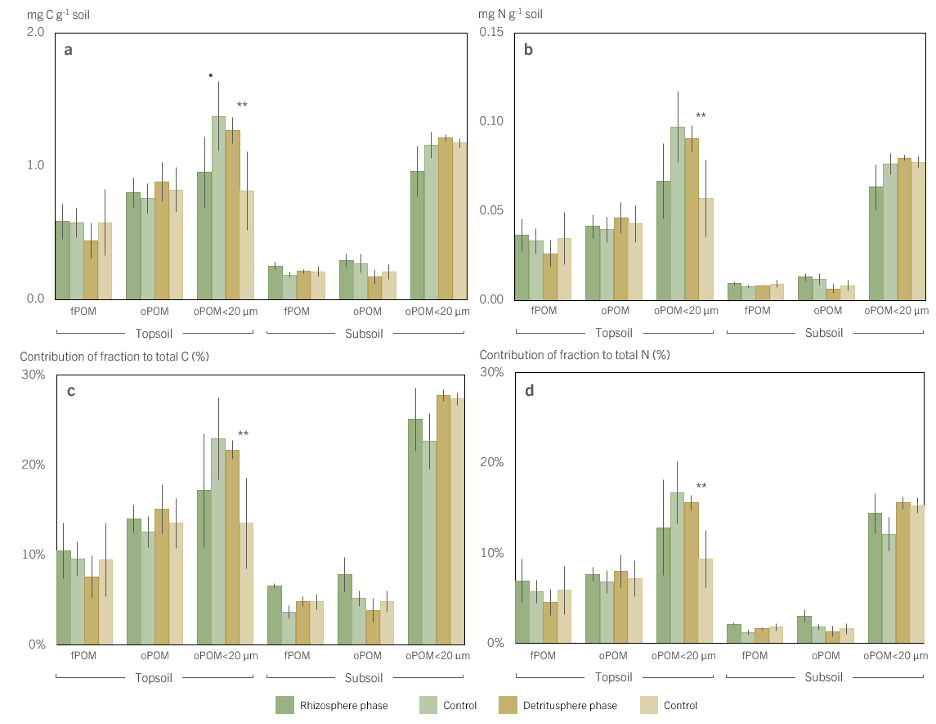
\includegraphics[width=1\textwidth]{img/M5-Figure_1.png}
	\caption{C and N contents in water-stable aggregate size classes. The contents of a) C and b) N (in \si{mg\,\gram^{-1}}\,fraction) in three water-stable aggregate-size classes and the concentrations of c) C and d) N (in \si{mg\,\gram^{-1}}\,soil) in the bulk soil. Green represents a living root phase (rhizosphere) and brown a decaying root phase (detritusphere) together with corresponding controls. Asterisks denote significant differences between rooted and control samples (\(.P < 0.1\), *\(P < 0.05\), **\(P < 0.01\), ***\(P < 0.001\)). Bars represent means \(\pm\)SD (\(n=6\) independent replicates).}
	\label{fig:M5-F1}
\end{figure}

Interestingly, contrary to the topsoil, the root effect was not isolated to macroaggregates in the subsoil, but also resulted in elevated C and N contents in larger microaggregates (\SIrange{53}{250}{\micro\metre}) compared to the corresponding controls (\num{5.49} in rooted samples and \SI{4.84}{mg\,C\,\gram^{-1}}\,soil in controls). In the topsoil, the effects of the living roots extended into the detritusphere phase in larger macroaggregates, with elevated C (\num{5.99} in rooted compared to \SI{5.27}{C\,\gram^{-1}} in controls, \(P=0.041\)) and N (\num{0.52} in rooted compared to \SI{0.45}{N\,\gram^{-1}} in controls, \(P=0.060\); Figure \ref{fig:M5-F1}c and Figure \ref{fig:M5-F1}d). This was not reflected in the subsoil.

\subsection{Elemental distribution in specific organic matter fractions}

Across treatments, the elemental compositions of the separated POM and MAOM fractions remained largely consistent, with almost no notable changes in their C and N contents around living or decaying roots.However, a clear change in the content of C and N (in \si{mg\,\gram^{-1}}\,soil) was observed in the oPOM<\SI{20}{\micro\metre} fraction within the topsoil (Figure \ref{fig:M5-F2}a and Figure \ref{fig:M5-F2}b). In the rhizosphere, the C content in oPOM<\SI{20}{\micro\metre} decreased slightly compared to unplanted controls (from \num{1.37} to \SI{0.95}{mg\,C\,\gram^{-1}}\,soil; \(P= 0.089\)). In the detritusphere, however, C in oPOM<\SI{20}{\micro\metre} was preserved around decaying roots compared to decreasing C contents of the same fractions in controls (\num{1.27} compared to \num{0.81}; \(P=0.025\); Figure \ref{fig:M5-F2}a and Figure \ref{fig:M5-F2}b). This was also reflected in the total amount of C allocated in oPOM<\SI{20}{\micro\metre} in the detritusphere (\num{38.07} compared to \SI{24.44}{mg\,C} in controls; \(P=0.052\)) and further emphasized by the maintained relative C and N contribution of the fraction around decaying roots in topsoil (Figure \ref{fig:M5-F2}c and Figure \ref{fig:M5-F2}d). This pattern was reversed around the living roots; although not significant, the total amount of C in oPOM<\SI{20}{\micro\metre} was slightly lower compared to the controls (\num{28.66} compared to \SI{41.30}{mg\,C}; \(P=0.187\)).

\begin{figure}[H]
	\centering
	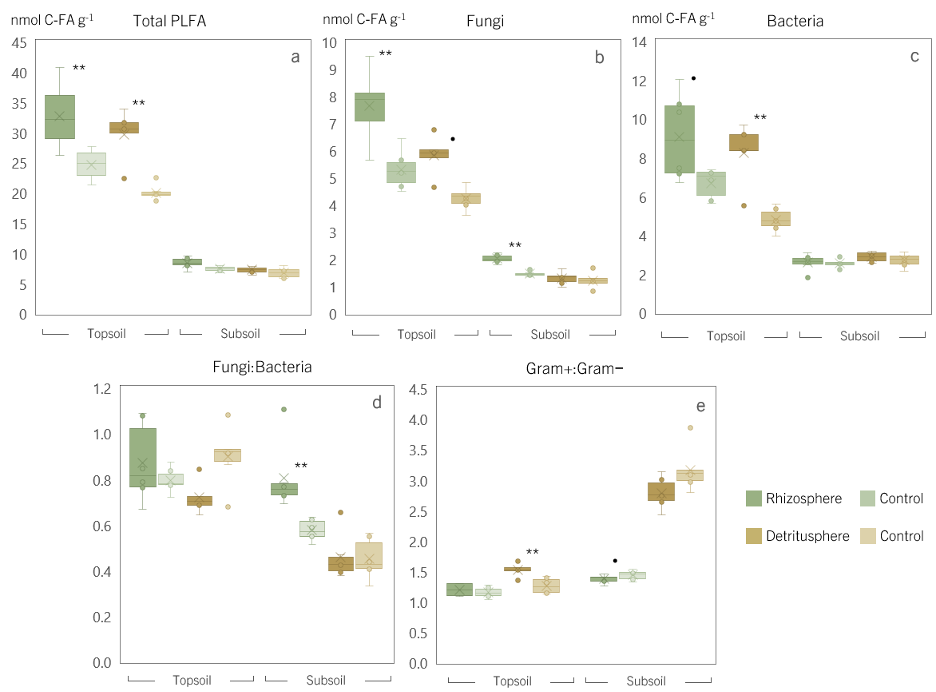
\includegraphics[width=1\textwidth]{img/M5-Figure_2.png}
	\caption{C and N contents in and contributions of particulate organic matter fractions. The content of a) C and b) N (in \si{mg\,\gram^{-1}}\,soil) and the contribution of c) C and d) N to the total stock (in \%) of organic matter fractions (fPOM, oPOM and oPOM<\SI{20}{\micro\metre}). Green represents a living root phase (rhizosphere) and brown a decaying root phase (detritusphere) together with corresponding controls in faded colors. Asterisks denote significant differences between rooted and control samples (\(.P < 0.1\), *\(P < 0.05\), **\(P < 0.01\), ***\(P < 0.001\)). Bars represent means \(\pm\)SD (\(n=3\) independent replicates).}
	\label{fig:M5-F2}
\end{figure}

The changes in the oPOM<\SI{20}{\micro\metre} fractions were not observed in the subsoil. Instead, there was a slight (non-significant) increase in the C contribution of the fPOM fraction in the subsoil rhizosphere (from \SI{3.63 \pm 0.74}{\percent} to \SI{6.59 \pm 0.27}{\percent}; \(P=0.154\); Figure \ref{fig:M5-F2}c). This led to increased C:N ratios of the fPOM fractions around living but also around decaying roots, from \num{24.37} to \num{26.88} in the rhizosphere (\(P=0.053\)) and from \num{22.91} to \num{25.36} in the detritusphere (\(P=0.086\)).

Although not significant, the fPOM fraction in the subsoil rhizosphere was further depleted in \textsuperscript{15}N (from \num{4.44} in controls to \SI{4.00}{\permil} in rooted samples; \(P < 0.001\)). In the detritusphere, this pattern was reversed, with the fraction instead enriched in \textsuperscript{15}N (from \num{4.26} in controls to \SI{4.77}{\permil} in rooted samples; \(P < 0.001\)). In MAOM fractions, we did not determine any significant changes in the isotopic composition across treatments. The chemical composition of the separated POM fractions (determined via \textsuperscript{13}C CP-MAS NMR) showed no differences between treatments, with little to no effect of the living or decaying roots. Further, the integrated regions showed similar chemical composition of the fractions, not only between the incubation phases, but also between the substrates.

\subsection{Phospholipid fatty acid analysis}

Microbially derived FAs increased in the rhizosphere of the topsoil substrate (from \num{24.62} to \SI{32.66}{nmol\,C\text{-}FA\,\gram^{-1}}\,soil; \(P=0.005\)) into the detritusphere phase, with the elevated microbial abundance being maintained in rooted topsoil samples compared to controls (\num{29.64} versus \SI{20.00}{nmol\,C\text{-}FA\,\gram^{-1}}\,soil; \(P=0.002\); Figure \ref{fig:M5-F3}a). Around living roots, both fungi and bacteria increased uniformly in the topsoil (Figure \ref{fig:M5-F3}b and Figure \ref{fig:M5-F3}c), as reflected by the fungi:bacteria ratio, which remained similar to controls despite the overall increase in FAs (Figure \ref{fig:M5-F3}d). However, as decomposition progressed, the fungal abundance around decaying roots decreased, while bacterial abundance was maintained. This was associated with a relative increase in Gram-positive bacteria around the decaying roots, as reflected in the elevated Gram+:Gram- ratio (from \num{0.70} to \num{0.90}; \(P=0.009\); Figure \ref{fig:M5-F3}e). In the subsoil, fungal abundance increased significantly around living roots compared to controls (\(P=0.007\)), similar to the differences observed in topsoil, with a shift in the fungi:bacteria ratio from \num{0.58} to \num{0.75} (\(P=0.005\)). During the detritusphere phase, no difference between roots and controls was observed in the subsoil.


\begin{figure}[H]
	\centering
	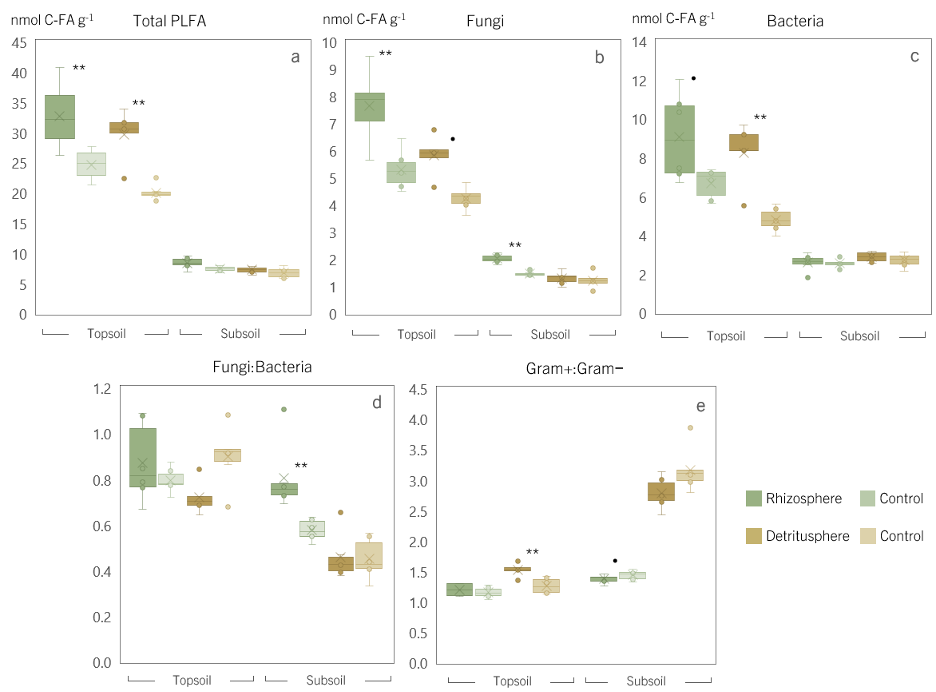
\includegraphics[width=1\textwidth]{img/M5-Figure_3.png}
	\caption{PLFA profiling of microbial community structure. The a) total content of extracted fatty acids (in \si{nmol\,C\text{-}FA\,\gram^{-1}}), the content of markers associated with b) fungi (\si{nmol\,C\text{-}FA\,\gram^{-1}}) and c) bacteria (\si{nmol\,C\text{-}FA\,\gram^{-1}}) and the d) fungi:bacteria ratio and e) Gram+:Gram− ratio in a topsoil and subsoil. Green boxes represent the living root phase (rhizosphere) and brown the decaying root phase (detritusphere) together with corresponding controls in faded colors. Asterisks denote significant differences between rooted and control samples (\(.P < 0.1\), *\(P < 0.05\), **\(P < 0.01\), ***\(P < 0.001\)). Box plots indicate medians (line) and means (x), where the first (Q1) and third (Q3) quartile are represented by the lower, respectively upper bounds of the box. Error bars represent the data range, bounded to \(1.5 \times (\text{Q3}-\text{Q1})\); (\(n = 6\) independent replicates).}
	\label{fig:M5-F3}
\end{figure}

\section{Discussion}

The purpose of this study was to investigate how plant roots drive soil structure formation and SOM build-up during early stages of soil development in a dryland soil system. The experiment was designed to follow the natural undisturbed succession from rhizosphere to detritusphere, aiming at capturing possible legacy effects from the rhizosphere influencing the development of the detritusphere. This allowed for the direct observation of changes in SOM formation, aggregation, and microbial community composition during phases where C inputs were primarily derived from either active rhizodeposition ('rhizosphere phase') or decaying root litter inputs ('detritusphere phase'). We hereby demonstrate how root-microbe-soil interactions change during the transition from rhizosphere to detritusphere, and how these processes are partially constrained—or counterbalanced—depending on the soil substrate in which the roots grow and later decompose.

\subsection{The rhizosphere: rhizodeposition as C input}

In the studied dryland soil, roots induced a shift in soil aggregation in the rhizosphere, leading to an increased contribution of water-stable macroaggregates to the total mass and an increased allocation of C and N to macroaggregates in both topsoil and subsoil (Figure \ref{fig:M5-F1}c and Figure \ref{fig:M5-F4}d; Figure \ref{fig:figure_4a_label}). This root effect is consistent with the well-established consensus that plant roots drive the formation of coarser aggregate structures, for example via root-derived gluing agents or direct entanglement of soil particles \citep{Tisdall1982, Six2004, Angst2018, Gregory2022}.

\begin{figure}[H]
	\centering
	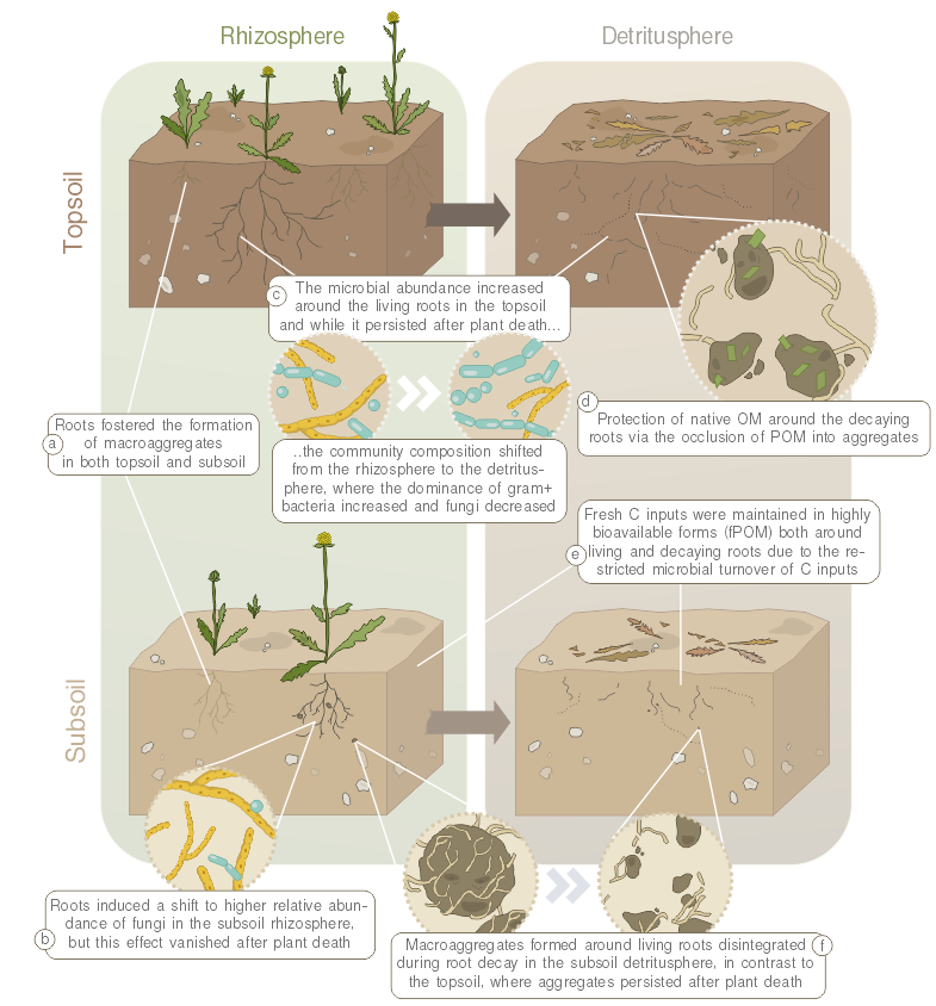
\includegraphics[width=1\textwidth]{img/M5-Figure_4.png}
	\caption{a) Living roots fostered the formation of macroaggregates in both topsoil and subsoil, and b) induced a change in the microbial community composition in the subsoil towards a higher relative abundance of fungi. This was not reflected in the topsoil, where c) the microbial abundance instead increased uniformly in the rhizosphere without structural changes in the community. While the increased total microbial abundance was maintained in the detritusphere, the composition changed as Gram+ bacteria outcompeted fungi. Around decaying roots in the topsoil, d) OM was protected in aggregates via the formation of occluded POM (oPOM<\SI{20}{\micro\metre}) and in the subsoil, e) the slower microbial C turnover resulted in an accumulation of fresh C inputs in highly bioavailable forms (fPOM) around both living and decaying roots. While the root-induced macroaggregates persisted after plant death in the topsoil, f) the aggregates disintegrated in the subsoil around the decaying roots.}
	\label{fig:M5-F4}
\end{figure}

The pioneer plant shaped the composition of the microbial community around the living roots. Driven by the easily available OM from the rhizodeposits, the total microbial abundance increased significantly in the topsoil rhizosphere (Figure \ref{fig:M5-F3}a). Interestingly, both fungi and bacteria increased similarly (Figure \ref{fig:M5-F3}b and Figure \ref{fig:M5-F3}c), meaning that the overall community structure remained unaffected by rooting (Figure \ref{fig:M5-F4}c). In contrast, there was no substantial increase in total microbial abundance in the subsoil rhizosphere. Instead, we determine a pronounced community shift towards a higher relative abundance of fungi in the subsoil (Figure \ref{fig:M5-F3}b), while bacterial abundance remained unaffected by the roots (Figure \ref{fig:M5-F4}b). These findings are in accordance with the widely accepted notion that conditions in the rhizosphere favor fungi over other microbial groups \citep{Butler2003, Brant2006, Denef2009}. This could be due to the lower content and diversity of SOM (including native OM) in the subsoil, where the filamentous growth of the fungal mycelium benefit fungi in gaining access to heterogeneously distributed OM resources, compared to bacteria with rather restricted motility in the soil \citep{DeBoer2005}.

Roots grown in the subsoil were of lower litter quality (higher lignin\textsubscript{NMR}:N ratio) compared to in the topsoil, and as fungi are adapted to assimilate more complex C resources from litter, this may have further amplified the distinction of fungi in the subsoil \citep{Poll2006}. Moreover, it is possible that this shift towards increased fungal dominance in the subsoil contributes not only to root-induced macroaggregation, but also to the observed microaggregation in the subsoil rhizosphere, which was not observed in the topsoil (Figure \ref{fig:M5-F1}a and Figure \ref{fig:M5-F1}b). Fungal hyphae as vectors for macroaggregation have been widely reported (e.g., \citeauthor{Bossuyt2001}, \citeyear{Bossuyt2001}; \citeauthor{Lehmann2020}, \citeyear{Lehmann2020}; \citeauthor{Bucka2021}, \citeyear{Bucka2021}), but evidence for the processes associated with fungal-induced microaggregation remains scarce. \citet{Vidal2018} show how hyphae are in fact closely linked to soil microstructure formation directly at the root-soil interface. \citet{Rillig2006} further point to mycorrhizal fungal mycelial products as drivers of the formation of smaller aggregates. As arbuscular mycorrhizal colonization has been reported for the pioneer species used in this study growing in adjacent study sites (\textit{Helenium aromaticum}; \citeauthor{Dhillion1995}, \citeyear{Dhillion1995}), mycelial byproducts and mutualistic plant-microbial interactions may be a contributing factor to the increased microaggregation in the subsoil. The increased fungal abundance in the subsoil rhizosphere is consistent with the findings of \citet{Baumert2021} and overall emphasizes fungi as key players in the assimilation of root-derived C compounds in the subsoil.

In association with the increased fungal dominance in the subsoil rhizosphere, we determine that the effect of the roots on aggregation was not isolated to macroaggregates in the subsoil but extended to larger microaggregates, where C and N contents were elevated compared to the controls (Figure \ref{fig:M5-F1}a and Figure \ref{fig:M5-F1}b), which further highlights the importance of labile root-derived gluing agents for aggregate formation during early rhizosphere development in C poor subsoils \citep{Baumert2018}.

\subsection{The detritusphere: root litter as C input}

After plant death, as the rhizosphere transitioned to a detritusphere, the initially formed root-induced macroaggregation remained in the topsoil but entirely disintegrated in the subsoil. The overall lack of aggregate stability over time is consistent with observations showing that a continuous input of OM is necessary to maintain aggregate structures, and that the disintegration of macroaggregates begins during early stages of decomposition when available C sources and microbial activity decline (e.g., \citeauthor{Golchin1997}, \citeyear{Golchin1997}; \citeauthor{Helfrich2008}, \citeyear{Helfrich2008}). In the present study, disintegration of newly formed aggregates was indeed particularly pronounced in the C poor subsoil (Figure \ref{fig:M5-F4}f), which is supported by the work of \citet{Bucka2021}, who report low mechanical stability of newly formed macroaggregates after OM addition in initial soils compared to greater retained aggregate stability in mature soils \citep{Felde2020}. This suggests that aggregates initially formed in the rhizosphere are only loosely connected, and that a living root system---or continuous C input---is a prerequisite for aggregate formation and persistence in soil systems with otherwise limited C inputs. Furthermore, these results suggest that a certain 'backbone' of native C, as in the topsoil, is required for long-term aggregate stabilization in arid soil systems. The difference between topsoil and subsoil may have been further amplified by the fact that roots grown in subsoil had lower litter quality (higher C:N and lignin\textsubscript{NMR}:N ratio; Table \ref{tab:M5-T1}; \citeauthor{Walela2014}, \citeyear{Walela2014}) compared to those grown in topsoil, further reinforcing the limiting conditions for microbial activity.

The transition from a living to a decaying root system, and thereby from C inputs dominated by low molecular weight compounds to more complex structural litter-derived C sources, shaped the composition and structure of the microbial community. The relative dominance of Gram+ over Gram- bacteria increased distinctively in the detritusphere of both soil substrates (Figure \ref{fig:M5-F3}e). This was likely driven by the increasing complexity of the litter resources as the decomposition progressed (e.g., as indicated by increasing (Ac/Al)\textsubscript{V} ratios; Table \ref{tab:M5-T1}), favoring Gram+ bacteria which are specialized in the processing of complex C sources \citep{Fanin2019, Denef2009, Butler2003}. This is supported by \citet{Shi2018}, who show how the microbial genetic potential to decompose complex macromolecular compounds increases in the absence of living roots, while root exudates in the rhizosphere instead promote the development of a microbial community with increased capacity to utilize low molecular weight compounds. This underscores how the presence of living and decaying roots modulates litter decomposition through alterations in microbial functionality. Furthermore, \citet{Nuccio2020} specifically describe how both temporal and spatial niche microbial coexistence is fostered in the combined rhizosphere-detritusphere, which opens up important future research opportunities in the transition zone from rhizosphere to detritusphere and highlights need for further research including microbial functional traits.

Interestingly, the shift in the microbiome around decaying roots in the topsoil was not associated with a change in overall abundance---in fact, abundance prevailed from the rhizosphere to the detritusphere phase, while decreasing in the corresponding controls (Figure \ref{fig:M5-F3}a). Consequently, despite the resource-limited conditions as decomposition progressed, litter-derived C inputs were sufficient to maintain microbial abundance, but the conditions favored those microbial groups specialized in utilizing complex C sources.

Another shift in microbial community structure in the detritusphere was observed in fungi, where both total fungal abundance and relative abundance to bacteria decreased, particularly so in the subsoil (Figure \ref{fig:M5-F3}b and Figure \ref{fig:M5-F3}d). The shift towards bacterial dominance in the detritusphere contrasts with the general notion of fungi as key players in litter decomposition \citep{Williams2006, Voriskova2013}. As PLFA profiles were only quantified at one point during the decomposition process in the present study, this represents only a snapshot of the ongoing succession of the microbial community involved in decomposition. \citet{Herman2012} found that fungal dominance during litter decomposition decreased rapidly after 21 days, after which Gram+ and Gram- increased. \citet{Voriskova2013} further emphasized the succession of the fungal community during decomposition, with different fungal taxa being highly abundant only during short periods. Thus, our results do not necessarily exclude fungal involvement in the initial stages of litter decomposition, but rather point to the increasing importance of bacteria during the late stages of decomposition, when labile litter components are depleted. This is supported by \citet{Esperschuetz2011} showing how Gram+ outcompete fungi in litter degradation in resource-limited systems where N is scarce. The retreat of fungi in the developed detritusphere in subsoil equates to the loss of the hyphal networks that enmeshed soil particles, which may cause the disintegration of aggregates around the decaying roots. This underlines the direct involvement of hyphae as a temporary binding agent in the rhizosphere that does not persist into the detritusphere \citep{Six2004}.

\subsection{Elemental composition of rhizosphere and detritusphere}

Contrary to our hypothesis, roots had no notable effects on total C and N contents in the bulk soil in the rhizosphere in either of the two soil substrates. It is possible that root inputs to the system were minor in comparison with other soil C pools, or that the inputs were rapidly processed by the stimulated microbial activity in the vicinity of the roots. Given the enhanced microbial abundance and changed community composition around the roots (Figure \ref{fig:M5-F3}), the second option appeared to be more likely. Nevertheless, it should be noted that the entire, thoroughly rooted pot was considered as 'rhizosphere' in the present study. Indeed, there is no clear definition of the spatial extent of the rhizosphere or where the boundaries of the rhizosphere are, as it depends on the parameters studied \citep{Kuzyakov2019}. However, most root-driven processes are concentrated in the immediate soil volume around the roots and diluted in the surrounding soil. For example, microbial abundance has been shown to be concentrated in the first \SIrange{1}{2}{\milli\metre} around the roots \citep{Marschner2012}, and rhizodeposits may have restricted dispersal potential from the immediate soil volume around the roots \citep{Kuzyakov2019}. This means that certain root effects may have been overseen, or diluted, given the large soil volume representing the rhizosphere. Under these circumstances, \textsuperscript{13}C labeling of the pioneer plants might have facilitated the quantification of small-scale elemental changes, thereby allowing a more detailed understanding of the fate of root-derived C in the soil, both in the rhizosphere and the subsequent detritusphere \citep{Teixeira2024}.

\subsection{Changes in POM around living and decaying roots}

Surprisingly, neither living nor decaying roots affected the composition of POM and MAOM, as evidenced by consistent C and N contents and comparable chemical compositions in all fractions. In the topsoil, however, occluded C as oPOM<\SI{20}{\micro\metre} and the contribution of this fraction to total C and N were clearly affected---albeit in contrasting ways between the rhizosphere and the detritusphere (Figure \ref{fig:M5-F2}). In the soil around the living root system, a slight decrease in occluded C was observed compared to the control, suggesting increased aggregate turnover around the roots \citep{Wang2020}. Root-induced breakdown of aggregates, combined with stimulated microbial activity around the roots resulting in an enhanced rhizosphere priming effect, could be contributing factors to the release and ultimate loss of bioavailable POM in the rhizosphere \citep{Cheng2009}. Around the decaying roots, the pattern was reversed, where instead an accumulation of occluded C (oPOM<\SI{20}{\micro\metre}) was determined (Figure \ref{fig:M5-F4}d). This highlights decaying roots as a prerequisite for the formation of occluded POM and shows how decaying litter surfaces in the detritusphere represent functional components that facilitate aggregate formation, directly contributing to the long-term stabilization of organic C in the soil \citep{Witzgall2021}.

In the subsoil, we observed elevated C:N ratios in the fPOM fractions in both the rhizosphere and detritusphere compared to unplanted controls Figure \ref{fig:M5-F4}e). During the rhizosphere phase, this was further associated with \textsuperscript{15}N depletion, indicating fresh C inputs into the fraction, as the opposite---increasing aliphaticity of OM---would otherwise lead to \textsuperscript{15}N accumulation \citep{Kramer2003}. This means that fresh C inputs remained in highly bioavailable forms (i.e., not occluded into aggregates or associated with mineral surfaces) and did not undergo notable microbial transformation during the course of both incubation phases. This phenomenon was only observed in subsoil, as there was no evidence of fresh C inputs in the fPOM fraction in the topsoil. This difference between the soil substrates can be attributed to restricted microbial abundance in the subsoil, resulting in slower C turnover compared to the topsoil where labile inputs were rapidly transformed. This may, in part, be related to the chemistry of the plant tissue in the subsoil, where roots were of lower biochemical quality compared to those in the topsoil (broader C:N ratios and elevated lignin\textsubscript{NMR}:N ratios; Table \ref{tab:M5-T1}; \citeauthor{Walela2014}, \citeyear{Walela2014}). These findings highlight the limiting conditions for microbial activity and suggest that lower quality litter is less preferred as a nutrient source for microbial decomposers. Collectively, these observations underscore the importance of roots as a critical source of POM in dryland subsoils, with legacy effects that can persist even after plant death \citep{Angst2016}. Furthermore, they emphasize how the litter chemistry of OM inputs shapes microbial community composition, with implications for aggregate formation.

\section{Conclusion}

In this study, we explore the interaction between plant roots, microorganisms, and soil during the succession from a rhizosphere to a root detritusphere in a dryland topsoil and subsoil. Our results highlight the fundamental role of roots in driving soil structure formation, microbial succession, and OM formation during the early stages of soil development. While we found root-induced macroaggregation in the topsoil, the effect of roots was extended to both increased macro- and micro-aggregates in the subsoil, presumably facilitated by fungal hyphae in the subsoil rhizosphere. However, with plant death, as the rhizosphere transitioned to a detritusphere, the newly formed aggregates disintegrated in the subsoil, underscoring the critical importance of continuous OM inputs for maintaining more persistent aggregate structures in C-poor subsoils. The transition to a detritusphere was further associated with a clear decline in fungal abundance and an increased dominance of Gram+ bacteria, emphasizing their role in mineralizing increasingly complex C resources in the developing detritusphere in dryland soils. Conversely, we found legacy effects of living roots imprinted in the topsoil, as macroaggregates formed within the rhizosphere persisted after plant death, and the microbiome developed around living roots was maintained in the detritusphere. While we found no changes in MAOM around the roots, we highlight the build-up of occluded POM facilitated by decaying root litter in the topsoil, underscoring the influence of root residues on SOM formation and persistence within the root detritusphere. Our work thus highlights the intricate interactions of plants, microorganisms, and soil particles in the vicinity of living and decaying roots in dryland soil systems, and how the biogeochemical processes involved are regulated by the soil substrate in which the roots grow and decompose. Our results further underscore the importance of encompassing the \textit{in situ} transition from living to decaying roots to advance our understanding of the dynamics of the legacy from rhizosphere and detritusphere.

\section*{CRediT authorship contribution statement}

\begin{description}
    \item[K. Witzgall:] Writing- review \& editing, Writing- original draft, Visualization, Methodology, Investigation, Formal analysis, Data curation, Conceptualization.
    \item[F.A. Steiner:] Writing- review \& editing, Writing- original draft, Investigation, Formal analysis, Data curation, Conceptualization.
    \item[B.D. Hesse:] Writing- review \& editing, Investigation, Data curation.
    \item[N. Riveras-Mu{\~n}oz:] Writing- review \& editing, Methodology, Data curation.
    \item[V. Rodr{\'\i}guez:] Writing- review \& editing, Methodology, Data curation. % Assuming accent on i
    \item[P.P.C. Teixeira:] Writing- review \& editing, Validation, Investigation.
    \item[M. Li:] Methodology.
    \item[R. Oses:] Writing- review \& editing, Conceptualization.
    \item[O. Seguel:] Writing- review \& editing, Conceptualization.
    \item[S. Seitz:] Writing- review \& editing, Conceptualization.
    \item[D. Wagner:] Writing- review \& editing, Supervision, Conceptualization.
    \item[T. Scholten:] Writing- review \& editing, Supervision, Resources, Funding acquisition, Conceptualization.
    \item[F. Buegger:] Writing- review \& editing, Formal analysis, Data curation.
    \item[G. Angst:] Writing- review \& editing, Supervision, Data curation, Conceptualization.
    \item[C.W. Mueller:] Writing- review \& editing, Validation, Supervision, Project administration, Methodology, Funding acquisition, Conceptualization.
\end{description}

\section*{Declaration of competing interest}

The authors declare that they have no known competing financial interests or personal relationships that could influence the work reported in this paper.

\section*{Data availability}

Data will be made available on request.

\section*{Acknowledgements}

The authors are grateful for the help and support of Maria Greiner and Nina Meschnark who supported the laboratory analyses. 
We also thank Josef Reischenbeck who built the machine used for aggregate fractionation. This work was financially supported by the German Research Foundation (DFG) as part of the 'EarthShape' priority program [grant no. MU3021/6-2; \url{www.earthshape.net}].

\section*{Supplementary data}

Supplementary data to this article can be found online at \url{https://doi.org/10.1016/j.soilbio.2024.109503}.

\bibliographystyle{natbib}
\bibliography{literatur-M5}


% --- Restore Original Chapter Formatting ---
% IMPORTANT: If you have any \chapter commands *after* this point
% (e.g., in \backmatter) that you *want* to have titles printed,
% you MUST restore the original definitions.
\makeatletter
\let\chapterlinesformat\originalchapterlinesformat
\let\chapterlineswithprefixformat\originalchapterlineswithprefixformat
\makeatother
% --- End of Restoration Code ---


% Other potential appendix sections:
% \chapter{Abbreviations \& Glossary}

\begin{longtable}[l]{p{.2\textwidth}p{.75\textwidth}}
% \endfirsthead
\endhead
\endfoot
% \endlastfoot
\textit{Bubble} & A structure in the graph topology that is being formed by variable sequence. It is defined as a closed subgraph with an upstream and downstream anchor \textit{node} and a set of \textit{nodes} in between them that represent variable sequence (\autoref{fig:basictube}). A looser formulation of this concept are \textit{snarls} \citep{Paten2018-qj}. \\
\textit{Core} & Part of a \textit{pan-genome} or \textit{pan-proteome} that is shared by all, or a large fraction of the accessions that are part of it \\
\textit{Core level} & A concept used by \textit{panSV} to describe the sharedness of a \textit{node} in the \textit{pan-genome}. The core level is defined as the number of genomes that contain the sequence stored in this \textit{node} and can differ from the number of \textit{paths} that traverse through it, e.g. in the case of a duplication event. \\
\textit{DAG} & Directed Acyclic Graph - A type of graph that prohibits loops in its structure to go back to previous \textit{nodes}. \\ 
\textit{Edge} & Connective feature of a genome graph that orders and connects the \textit{nodes}. \\
\textit{GFA} & Graphical Fragment Assembly - a file format to store graphs in a human readable form \citep{gfa_2021}. \\
\textit{HDR} & Highly Diverged Region - region in a genome that contains a multitude of smaller variants, above the average of the surrounding sequence. As defined by the pairwise variant detection tool SyRI \citep{Goel2019-rx}. \\
\textit{InDel} & Insertion-Deletion variation events in a reference framework that induces the polarity of sequence being inserted, or deleted from it. This term is slowly being replaced by \textit{PAV}. \\
\textit{Mobilome} & Fraction of the genome that consists of mobile elements such as \textit{TEs}. \\
\textit{MUM} & Maximal Unique Match - largest possible unique alignment between sequences \\
\textit{Node} & Element of a genome graph that stores the sequence. \\
\textit{OG} & Orthogroup - Group of orthologous genes. \\
\textit{Path} & Colored traversal through a set of consecutive \textit{nodes}, and \textit{edges} of a graph. A path represents longer sequences in the graph, such as the input genomes. By following it through the graph the full sequence can be recovered. \\
\textit{Pan-genome} & Combined collection of genetic sequence of multiple individuals to represent a larger population. \\
\textit{Pan-proteome} & Collection of genes, or transcripts from multiple individuals that represent an enriched collection and the frequency of their occurrence in a larger population. \\
\textit{PAV} & Presence-Absence variation events. A type of genetic variation where sequence has been gained or lost. \\
\textit{Private} &Part of a \textit{pan-genome} or \textit{pan-proteome} that is shared by no other, or very few other individuals. \\
\textit{Shell} & Part of a \textit{pan-genome} or \textit{pan-proteome} that is niether \textit{core}, nor \textit{private}. \\
\textit{Snarl} & A structure in the graph topology that represents variable sequence in the graph. In contrast to a \textit{bubble} this structure does not have to be a closed subgraph with up- and downstream anchors, but can have additional connections into it, or lack one of the anchors \citep{Paten2018-qj}. \\
\textit{SNP} & Single-Nucleotide-Polymorphism - Variation between two DNA sequences where a single base is replaced by another single base. \\
\textit{Superbubble} & A large substructure of the graph. It follows the definition of a \textit{bubble}, but contains at least one smaller \textit{bubble} inside. \\
\textit{SV} & Structural Variation - Large sequence variation that alters the structure of the genome, for example PAVs, duplications, or translocations. \\
\textit{TE} & Transposable Element - Mobile elements in the DNA sequence that are able to replicate themselves and insert into the genome. \\
\textit{Traversal} & A collection of consecutive \textit{nodes}, and \textit{edges} in a graph that has a defined start and end \textit{node}. 
\end{longtable}

 % If these use \chapter, their titles would also be suppressed unless placed after restoration
% \include{tex/Glossary}
% \chapter{Supplementary}

\section{Supplementary Figures}

\begin{figure}[h!]
	\centering
	\includegraphics[width=\textwidth]{img/sixRefCoordinates}
	\caption{\textbf{SixRef coordinates} - Geographic locations of the six accessions chosen for assembly.}
	\label{fig:sixRefCoords}
\end{figure}

\begin{figure}[h!]
	\centering
	\includegraphics[width=\textwidth]{img/dotplot}
	\caption{\textbf{Assembly dot-plots} - Synteny representation of the six \textit{de-novo} assemblies, based on \textit{minimap2} alignments with the \textit{TAIR10} reference genome to show the high level of synteny and reveal large scale inversions. Breakpoints are mostly located in the pericentromeric regions, together with a set of inversions.}
	\label{fig:dotplots}
\end{figure}

\begin{figure}[h!]
	\centering
	\includegraphics[width=\textwidth]{img/SyRIrear}
	\caption{\textbf{\textit{SyRI} rearrangements} - Large scale structural rearrangements detected by \textit{SyRI}. The majority of the chromosomes are highly collinear, and differences can mostly be observed in the pericentromeric regions.}
	\label{fig:SyRIrear}
\end{figure}

\begin{figure}[h!]
	\centering
	\includegraphics[width=\textwidth]{img/panSVbubbleCount}
	\caption{\textbf{\textit{panSV} bubbles} - Distribution of core levels of variable regions detected by \textit{panSV}. Most of the regions have core level 7 and only a smaller fraction is nested within them.}
	\label{fig:panSVbubbleCount}
\end{figure}

\begin{figure}[h!]
	\centering
	\includegraphics[width=0.85\textwidth]{img/TEcoverageHeat2}
	\caption{\textbf{TE node coverage} - Heat map of the coverage of nodes ($>$50 bp) that are annotated as containing a TE in at least one accession of the graph.}
	\label{fig:TEcoverageHeat}
\end{figure}

\begin{figure}[h!]
	\centering
	\includegraphics[width=0.85\textwidth]{img/orthogroupPanZscore}
	\caption{\textbf{Orthogroup Z-Score} - Z-Score matrix of the estimated copy numbers of orthogroups, based on the number coverage of the accessions mapped to the graph.}
	\label{fig:orthoPanZ}
\end{figure}

\FloatBarrier

\section{Supplementary Tables}

\begin{table}[h]
	\centering
	\caption{\textbf{Reference based variant calls} - Number and size of reference based variant calls, of the sixRef accessions, in comparison to the \textit{TAIR10} reference genome, made with three different approaches. Short-read based variant calls made as part of the 1001 Genomes Project, pairwise alignment based variants called using \textit{SyRI} from the \textit{de-novo} chromosome scaffolds aligned to the \textit{TAIR10} reference genome, graph based variants, extracted from the graph using \textit{vg deconstruct}. The variants were classified as \textit{SNPs} (one base pair replaced by another base pair), \textit{small variants} ($<$50bp), and \textit{large variants} ($\geq$ 50bp).}
	\resizebox{0.8\textwidth}{!}{
		\begin{tabular}{l|rrrrr}
			& \multicolumn{1}{l}{\# Variants} & \multicolumn{1}{l}{\% Variants} & \multicolumn{1}{l}{Size {[}Mb{]}} & \multicolumn{1}{l}{avg. size} & \multicolumn{1}{l}{median size} \\ \hline
			\multicolumn{6}{c}{Short-read based variants} \\ \hline
			Total & 1,570,148 & 100 & 1.7 & 1.1 & 1 \\
			\textit{SNP} & 1,443,401 & 91.9 & 1.4 & 1 & 1 \\
			\textit{small variant} & 126,747 & 8.1 & 0.2 & 1.8 & 3 \\
			\textit{large variant} & 0 & 0 & 0 & 0 & 0 \\ \hline
			\multicolumn{6}{c}{\textit{Pairwise alignment based variants}} \\ \hline
			Total & 2,589,009 & 100 & 8.2 & 3.2 & 1 \\
			\textit{SNP} & 1,963,863 & 75.9 & 2 & 1 & 1 \\
			\textit{small variant} & 609,648 & 23.6 & 1.5 & 2.5 & 1 \\
			\textit{large variant} & 15,498 & 0.6 & 4.8 & 306.7 & 1 \\ \hline
			\multicolumn{6}{c}{\textit{Graph based variants}} \\ \hline
			Total & 1,869,605 & 1 & 88.6 & 47.4 & 1 \\
			\textit{SNP} & 1,272,633 & 68.1 & 1.3 & 1 & 1 \\
			\textit{small variant} & 539,644 & 0.28.9 & 2.2 & 4 & 2 \\
			\textit{large variant} & 57,328 & 3.1 & 85.2 & 1486.5 & 154
		\end{tabular}
	}
	\label{tab:refGraphCalls}
\end{table}

\begin{table}[h]
	\centering
	\caption{\textbf{Variant call overlap} - Variants that did not intersect with all other sets were overlapped with the remaining variants of the sets. Variants were classified as \textit{small} ($<$50bp) and \textit{large} ($\geq$ 50bp). \textit{SNPs} were excluded.}
	\resizebox{0.8\textwidth}{!}{
		\begin{tabular}{l|rrrrl}
			& \multicolumn{2}{c}{small variants} & \multicolumn{2}{c}{large variants}& \\
			& \multicolumn{1}{l}{\# variants} & \multicolumn{1}{l}{\%Intersection} & \multicolumn{1}{l}{\# variants} & \multicolumn{1}{l}{\% Intersection} & Intersecting Sets \\ \hline
			1001G & 9,873 & 12.3 & \multicolumn{1}{l}{-} & \multicolumn{1}{l}{-} & \textit{SyRI} \\
			1001G & 44,293 & 55.4 & \multicolumn{1}{l}{-} & \multicolumn{1}{l}{-} & \textit{vg deconstruct} \\
			SyRi  & 27,290 & 4.9 & 4,849 & 31.3 & short-reads \\
			SyRi  & 110,919 & 19.7 & 6,904 & 44.6 & \textit{vg deconstruct} \\
			graph & 78,855 & 16 & 11,465 & 20 & short-reads \\
			graph & 112,561 & 22.8 & 11,807 & 20.6 & \textit{SyR}           
		\end{tabular}
	}
	\label{tab:refGraphCallComp}
\end{table}

\begin{sidewaystable}[h]
\centering
\caption{\textbf{\textit{auto-ant} sensitivity} - Features of each annotation intersecting with the annotated features in the \textit{araport11} reference annotation. Some features were removed from the table as they did not intersect with any of the annotations. Those features, and their occurences in \textit{araport11} were: lnc\_RNA (2455), miRNA (427), miRNA\_primary\_transcript (325), pseudogenic\_tRNA (27), rRNA (15), snoRNA (287), snRNA (82), transcript\_region (726), tRNA (689), antisense\_RNA (91)}
\resizebox{\textwidth}{!}{
	\begin{tabular}{l|r|rr|rr|rr|rr|rr|rr}
		& \multicolumn{1}{l}{\textit{araport11}} & \multicolumn{2}{l}{\textit{BUSCO retrained augustus}} & \multicolumn{2}{l}{\textit{LiftOff based augustus}}& \multicolumn{2}{l}{RNA-Seq supported augustus} & \multicolumn{2}{l}{\textit{SNAP}} & \multicolumn{2}{l}{\textit{cufflinks assembly}} & \multicolumn{2}{l}{combined evidenceModeler} \\
		Feature & \multicolumn{1}{l}{Feature count} & \multicolumn{1}{l}{Feature count} & \multicolumn{1}{l}{Sensitivity in \textit{araport11}} & \multicolumn{1}{l}{Feature count} & \multicolumn{1}{l}{Sensitivity in \textit{araport11}} & \multicolumn{1}{l}{Feature count} & \multicolumn{1}{l}{Sensitivity in \textit{araport11}} & \multicolumn{1}{l}{Feature count} & \multicolumn{1}{l}{Sensitivity in \textit{araport11}} & \multicolumn{1}{l}{Feature count} & \multicolumn{1}{l}{Sensitivity in \textit{araport11}} & \multicolumn{1}{l}{Feature count} & \multicolumn{1}{l}{Sensitivity in \textit{araport11}} \\ \hline
		CDS & 286355 & 201840 & 0.7049 & 252047 & 0.8802 & 250829 & 0.8759 & 206895 & 0.7225 & 175032 & 0.6112 & 248384 & 0.8674 \\
		exon & 200542 & 78245 & 0.3902 & 104870 & 0.5229 & 98845 & 0.4929 & 78428 & 0.3911                                       & 87987 & 0.4387 & 92489 & 0.4612 \\
		gene & 33246 & 466 & 0.014 & 438 & 0.0132 & 298 & 0.009 & 586 & 0.0176 & 3 & 0.00009  & 652 & 0.0196 \\
		protein & 48359 & 16652 & 0.3443 & 4897 & 0.1013 & 4963 & 0.1026 & 5308 & 0.1098 & 0 & 0 & 27729 & 0.5734 \\
		three\_prime\_UTR & 41127 & 489 & 0.0119 & 956 & 0.0232 & 869 & 0.0211 & 511 & 0.0124  & 793 & 0.0193 & 627 & 0.0152 \\
		five\_prime\_UTR & 46895 & 283 & 0.006 & 1406 & 0.03 & 1029 & 0.0219 & 301 & 0.0064 & 1010  & 0.0215 & 388 & 0.0083 \\
		mRNA & 52141 & 0 & 0 & 556 & 0.0107 & 355 & 0.0068 & 778 & 0.0149 & 3 & 0.00005 & 919 & 0.0176 \\
		ncRNA & 286 & 0 & 0 & 0 & 0 & 0 & 0 & 0 & 0 & 0 & 0 & 2 & 0.007 \\
		pseudogene & 952 & 4 & 0.0042 & 3 & 0.0032 & 1 & 0.0011 & 11 & 0.0116 & 0 & 0 & 12 & 0.0126 \\
		pseudogenic\_exon & 2058 & 141 & 0.0685 & 178 & 0.0865 & 328 & 0.1594 & 220 & 0.1069 & 261 & 0.1268 & 194 & 0.0943 \\
		pseudogenic\_transcript & 1100 & 4 & 0.0036 & 3 & 0.0027 & 1 & 0.0009 & 11 & 0.01 & 0 & 0 & 12 & 0.0109 \\
		transposable\_element & 31189 & 10 & 0.0003 & 4 & 0.0001 & 5 & 0.0002 & 5 & 0.0002 & 0 & 0 & 8 & 0.0003 \\
		transposable\_element\_gene & 3901 & 72 & 0.0185 & 14 & 0.0036 & 8 & 0.0021 & 155 & 0.0397 & 0 & 0 & 84 & 0.0215 \\
		transposon\_fragment & 34856 & 10 & 0.0003 & 4 & 0.0001 & 5 & 0.0001 & 5 & 0.0001 & 0 & 0 & 8 & 0.0002 \\
		uORF & 111 & 2 & 0.018 & 6 & 0.0541 & 1 & 0.009 & 7 & 0.0631 & 1 & 0.009 & 0 & 0 \\
		antisense\_lncRNA &  1424 & 0 & 0 & 1 & 0.0007 & 0 & 0 & 1 & 0.0007 & 0 & 0 & 0 & 0
	\end{tabular}
}
\label{tab:autoAntSensitivity}
\end{sidewaystable}

\begin{table}[h]
	\centering
	\caption{\textbf{RNA-Seq reads} - Raw count and fraction of RNA sequencing reads for each accession. The fraction always refers to the total number of raw reads.}
	\resizebox{\textwidth}{!}{
		\begin{tabular}{ll|rrrrrr}
			& & \multicolumn{1}{l}{AT1741} & \multicolumn{1}{l}{AT5784} & \multicolumn{1}{l}{AT6909}  & \multicolumn{1}{l}{AT6911} & \multicolumn{1}{l}{AT7186}   & \multicolumn{1}{l}{AT7213} \\ \hline
			Count & Raw Reads & 301,393,206 & 503,865,660 & 312,783,846 & 384,735,390 & 284,003,720 & 244,454,716 \\ \hline
			Fraction & Flower & 22.5 & 11 & 46.6 & 47.8 & 24.7 & 18.4 \\
			& Leaf &  22.8 &  12.4 & 19.4 & 15.1 & 15.1 & 31. \\
			& Roo & 27.4 & 61.9 & 19.4 & 28.2 & 25.8 & 32.2 \\
			& Seedling  & 27.4 & 14.7 &14.5 & 9 & 34.4 & 17.7 \\
			& Trimmed  & 88.3 & 94.5 &  95.3 &  91.6 &  91.7 & 92.6 \\
			& Mapped  & 45.3 & 37.8 & 64.2 & 36 & 51.5 & 58                                                
		\end{tabular}
	}
	\label{tab:RNAseqReads}
\end{table}

\begin{table}[h]
	\centering
	\caption{\textbf{Non-reference \textit{SyRI} intersection} - Intersection of non-reference sequences with calls made by \textit{SyRI}. Multiple events could be contained in one interval. I destinguished regions that were classified as not-aligned by \textit{SyRI} and all other variants $\geq$ 50 bp detected by \textit{SyRI}. The fraction relates to the total number of large non-reference sequences of the accession.}
	\resizebox{\textwidth}{!}{
		\begin{tabular}{l|rrr|rrr}
			& \multicolumn{3}{l}{\textit{SyRI} unaligned} & \multicolumn{3}{l}{\textit{SyRI} SVs} \\
			Accession & \multicolumn{1}{l}{\begin{tabular}[c]{@{}l@{}}non-ref\\ Regions\end{tabular}} & \multicolumn{1}{l}{\textit{SyRI} events} & \multicolumn{1}{l}{\begin{tabular}[c]{@{}l@{}}\% non-ref\\ Regions\end{tabular}} & \multicolumn{1}{l}{\begin{tabular}[c]{@{}l@{}}non-ref\\ Regions\end{tabular}} & \multicolumn{1}{l}{\textit{SyRI} events} & \multicolumn{1}{l}{\begin{tabular}[c]{@{}l@{}}\% non-ref\\ Regions\end{tabular}} \\ \hline
			AT1741 & 268 & 525 & 3.9 & 354 & 668 & 5.2 \\
			AT5784 & 313 & 586 & 4 & 478 & 782 & 6.1 \\
			AT6909 & 30 & 36 & 4.4 & 21 & 62 & 3.1 \\
			AT6911 & 365 & 682 & 3.9 & 503 & 845 & 5.4 \\
			AT7186 & 310 & 537 & 4.1 & 438 & 698 & 5.8 \\
			AT7213 & 303 & 588 & 4.1 & 421 & 748 & 5.60                                                                            
		\end{tabular}
	}
	\label{tab:nonRefSyRIisec}
\end{table}

\begin{table}[h]
	\centering
	\caption{\textbf{Graph mapping test graphs} - Statistics of the graphs used in the graph mapping evaluation. For each graph the sequence length, the sequence based multiple of the \textit{TAIR10} reference genome, the level of compression compared to the combined input genomes are shown. In addition the Number of nodes, and edges, as well as the edge number divided by node number.}
	\resizebox{\textwidth}{!}{
		\begin{tabular}{l|rrrrrr}
			& \multicolumn{1}{l}{Seq. Length {[}Mb{]}} & \multicolumn{1}{l}{Ref Fraction} & \multicolumn{1}{l}{Comp. Level} & \multicolumn{1}{l}{\# Nodes} & \multicolumn{1}{l}{\# Edges} & \multicolumn{1}{l}{Node Degree} \\ \hline
			\textit{Flat graph} & 119.7 & 1 & 0 & 3,829,320 & 3,829,313 & 1 \\
			\textit{VCF graph} & 220.4 & 1.8 & 25.76 & 5,601,134 & 8,307,979 & 1.5 \\
			\textit{Chrom graph} & 197.5 & 1.7 & 23.08 & 6,247,306 & 8,491,456 & 1.4 \\
			\textit{Linear graph}  & 195.5 & 1.6 & 22.86 & 6,282,045 & 8,540,670 & 1.4 \\
			\textit{Complex graph} & 168.80 & 1.4 & 19.73 & 6,694,806 & 9,147,110& 1.4                            
		\end{tabular}
	}
	\label{tab:testGraphs}
\end{table}

\begin{table}[h]
	\centering
	\caption{\textbf{Graph mapping statistics} - Statistics of mappings to the different test graphs using the prepared graphs with increasing complexity. Not all mapping algorithms could be used on all graphs. Either due to the method (\textit{vg inject}, \textit{bwa mem}), or the excessive run time and resource consumption (\textit{vg map}).}
	\resizebox{\textwidth}{!}{
		\begin{tabular}{ll|rrr}
			& & \multicolumn{1}{l}{\begin{tabular}[c]{@{}l@{}}Mapped reads {[}\%{]}\end{tabular}} & \multicolumn{1}{l}{\begin{tabular}[c]{@{}l@{}}Covered graph\\sequence {[}\%{]}\end{tabular}} & \multicolumn{1}{l}{Covered bases {[}Mb{]}} \\ \hline
			\textit{Flat graph} & \textit{bwa mem} & 96.16 & 95.42 & 114.2 \\
			& \textit{vg map} & 96.01 & 95.4 & 114.2 \\
			& \textit{vg giraffe} & 96.1 & 94.9 & 113.6 \\
			& \textit{graphAligner} & 56.79 & 97.1 & 116.2 \\
			& \textit{vg inject} & 96.16 & 95.42 & 114.2 \\ \hline
			\textit{VCF graph} & \textit{bwa mem} & \multicolumn{1}{c}{-} & \multicolumn{1}{c}{-} & \multicolumn{1}{c}{-} \\
			& \textit{vg map} & 96.51 & 61.98 & 136.6 \\
			& \textit{vg giraffe} & 97.46 & 62.01 & 136.7 \\
			& \textit{graphAligner} & 44.44 & 80.39 & 177.2 \\
			& \textit{vg inject} & \multicolumn{1}{c}{-} & \multicolumn{1}{c}{-} & \multicolumn{1}{c}{-} \\ \hline
			\textit{Chrom graph} & \textit{bwa mem} & \multicolumn{1}{c}{-} & \multicolumn{1}{c}{-} & \multicolumn{1}{c}{-} \\
			& \textit{vg map} & 56.24 & 30.49 & 60.2 \\
			& \textit{vg giraffe}   & 97.69 & 68.27 & 134.9 \\
			& \textit{graphAligner} & 43.13 & 77.88 & 153.9 \\
			& \textit{vg inject} & \multicolumn{1}{c}{-} & \multicolumn{1}{c}{-} & \multicolumn{1}{c}{-} \\ \hline
			\textit{Linear graph} & \textit{bwa mem} & \multicolumn{1}{c}{-} & \multicolumn{1}{c}{-} & \multicolumn{1}{c}{-} \\
			& \textit{vg map} & \multicolumn{1}{c}{-} & \multicolumn{1}{c}{-} & \multicolumn{1}{c}{-} \\
			& \textit{vg giraffe} & 97.67 & 68.5 & 133.9 \\
			& \textit{graphAligner} & 43.06 & 78.06 & 152.6 \\
			& \textit{vg inject} & 97.11 & 72.36 & 141.5 \\ \hline
			\textit{Complex graph} & \textit{bwa mem} & \multicolumn{1}{c}{-} & \multicolumn{1}{c}{-} & \multicolumn{1}{c}{-} \\
			& \textit{vg map} & \multicolumn{1}{c}{-} & \multicolumn{1}{c}{-} & \multicolumn{1}{c}{-} \\
			& \textit{vg giraffe} & 73.37 & 42.27 & 71.3 \\
			& \textit{graphAligner} & 41.01 & 81.81 & 138.1 \\
			& \textit{vg inject} & 97.12 & 75.4 & 127.2                                                             
		\end{tabular}
	}
	\label{tab:graphMappingStats}
\end{table}

\begin{table}[h]
	\centering
	\caption{\textbf{Mapping population} - List of all accessions and their admixture group, that are part of the mapping population.}
	\resizebox{\textwidth}{!}{
		\begin{tabular}{rl|rl|rl|rl|rl|rl|rl|rl|rl}
			\multicolumn{1}{l}{ID} & admixture group & \multicolumn{1}{l}{ID} & admixture group & \multicolumn{1}{l}{ID} & admixture group & \multicolumn{1}{l}{ID} & admixture group & \multicolumn{1}{l}{ID} & admixture group         & \multicolumn{1}{l}{ID} & admixture group         & \multicolumn{1}{l}{ID} & admixture group & \multicolumn{1}{l}{ID} & admixture group & ID                       & admixture group \\ \hline
			10022                  & admixed         & 9824                   & admixed         & 5907                   & central\_europe & 9772                   & central\_europe & 6909                   & germany                 & 9646                   & italy\_balkan\_caucasus & 6115                   & south\_sweden   & 9841                   & spain           & \multicolumn{1}{r}{88}   & western\_europe \\
			1313                   & admixed         & 9830                   & admixed         & 5921                   & central\_europe & 9774                   & central\_europe & 6915                   & germany                 & 9647                   & italy\_balkan\_caucasus & 6118                   & south\_sweden   & 9843                   & spain           & \multicolumn{1}{r}{9298} & western\_europe \\
			1317                   & admixed         & 9831                   & admixed         & 5950                   & central\_europe & 9775                   & central\_europe & 6922                   & germany                 & 9648                   & italy\_balkan\_caucasus & 6119                   & south\_sweden   & 9844                   & spain           & \multicolumn{1}{r}{9312} & western\_europe \\
			2016                   & admixed         & 9835                   & admixed         & 5984                   & central\_europe & 9776                   & central\_europe & 6940                   & germany                 & 9649                   & italy\_balkan\_caucasus & 6122                   & south\_sweden   & 9845                   & spain           & \multicolumn{1}{r}{9314} & western\_europe \\
			2202                   & admixed         & 9838                   & admixed         & 5993                   & central\_europe & 9777                   & central\_europe & 6945                   & germany                 & 9651                   & italy\_balkan\_caucasus & 6123                   & south\_sweden   & 9846                   & spain           & \multicolumn{1}{r}{932}  & western\_europe \\
			2276                   & admixed         & 9839                   & admixed         & 6008                   & central\_europe & 9778                   & central\_europe & 6982                   & germany                 & 9653                   & italy\_balkan\_caucasus & 6124                   & south\_sweden   & 9848                   & spain           & \multicolumn{1}{r}{9503} & western\_europe \\
			2317                   & admixed         & 9849                   & admixed         & 6296                   & central\_europe & 9779                   & central\_europe & 6997                   & germany                 & 9655                   & italy\_balkan\_caucasus & 6134                   & south\_sweden   & 9850                   & spain           & \multicolumn{1}{r}{9517} & western\_europe \\
			265                    & admixed         & 9858                   & admixed         & 6390                   & central\_europe & 9780                   & central\_europe & 7000                   & germany                 & 9656                   & italy\_balkan\_caucasus & 6141                   & south\_sweden   & 9852                   & spain           & \multicolumn{1}{r}{9569} & western\_europe \\
			5151                   & admixed         & 9877                   & admixed         & 6396                   & central\_europe & 9781                   & central\_europe & 7002                   & germany                 & 9657                   & italy\_balkan\_caucasus & 6149                   & south\_sweden   & 9855                   & spain           & \multicolumn{1}{r}{9571} & western\_europe \\
			5165                   & admixed         & 9881                   & admixed         & 6424                   & central\_europe & 9782                   & central\_europe & 7008                   & germany                 & 9658                   & italy\_balkan\_caucasus & 6191                   & south\_sweden   & 9856                   & spain           & \multicolumn{1}{r}{9578} & western\_europe \\
			5720                   & admixed         & 9890                   & admixed         & 6445                   & central\_europe & 9784                   & central\_europe & 7014                   & germany                 & 9659                   & italy\_balkan\_caucasus & 6192                   & south\_sweden   & 9857                   & spain           & \multicolumn{1}{r}{9585} & western\_europe \\
			5757                   & admixed         & 9892                   & admixed         & 6903                   & central\_europe & 9785                   & central\_europe & 7031                   & germany                 & 9660                   & italy\_balkan\_caucasus & 6203                   & south\_sweden   & 9859                   & spain           & \multicolumn{1}{r}{9590} & western\_europe \\
			5768                   & admixed         & 9894                   & admixed         & 6919                   & central\_europe & 9786                   & central\_europe & 7033                   & germany                 & 9661                   & italy\_balkan\_caucasus & 6413                   & south\_sweden   & 9860                   & spain           & \multicolumn{1}{r}{9599} & western\_europe \\
			5772                   & admixed         & 9897                   & admixed         & 6951                   & central\_europe & 9787                   & central\_europe & 7036                   & germany                 & 9697                   & italy\_balkan\_caucasus & 6974                   & south\_sweden   & 9861                   & spain           & \multicolumn{1}{r}{9809} & western\_europe \\
			5784                   & admixed         & 9906                   & admixed         & 6956                   & central\_europe & 9788                   & central\_europe & 7062                   & germany                 & 9698                   & italy\_balkan\_caucasus & 7013                   & south\_sweden   & 9864                   & spain           & \multicolumn{1}{r}{9823} & western\_europe \\
			5811                   & admixed         & 9924                   & admixed         & 6957                   & central\_europe & 9789                   & central\_europe & 7094                   & germany                 & 9699                   & italy\_balkan\_caucasus & 7164                   & south\_sweden   & 9866                   & spain           & \multicolumn{1}{r}{9826} & western\_europe \\
			5822                   & admixed         & 9932                   & admixed         & 6975                   & central\_europe & 9790                   & central\_europe & 7102                   & germany                 & 9700                   & italy\_balkan\_caucasus & 7343                   & south\_sweden   & 9867                   & spain           & \multicolumn{1}{r}{9827} & western\_europe \\
			6042                   & admixed         & 9933                   & admixed         & 6976                   & central\_europe & 9791                   & central\_europe & 7117                   & germany                 & 9701                   & italy\_balkan\_caucasus & 7346                   & south\_sweden   & 9868                   & spain           & \multicolumn{1}{r}{9828} & western\_europe \\
			6434                   & admixed         & 14312                  & asia            & 6979                   & central\_europe & 9792                   & central\_europe & 7119                   & germany                 & 9703                   & italy\_balkan\_caucasus & 7354                   & south\_sweden   & 9870                   & spain           & \multicolumn{1}{r}{9847} & western\_europe \\
			6830                   & admixed         & 14313                  & asia            & 6984                   & central\_europe & 9793                   & central\_europe & 7125                   & germany                 & 9704                   & italy\_balkan\_caucasus & 8234                   & south\_sweden   & 9873                   & spain           & \multicolumn{1}{r}{9851} & western\_europe \\
			6898                   & admixed         & 14314                  & asia            & 7025                   & central\_europe & 9794                   & central\_europe & 7133                   & germany                 & 9705                   & italy\_balkan\_caucasus & 8237                   & south\_sweden   & 9874                   & spain           & \multicolumn{1}{r}{9853} & western\_europe \\
			6907                   & admixed         & 14315                  & asia            & 7103                   & central\_europe & 9795                   & central\_europe & 7143                   & germany                 & 9706                   & italy\_balkan\_caucasus & 8307                   & south\_sweden   & 9876                   & spain           & \multicolumn{1}{r}{9854} & western\_europe \\
			6920                   & admixed         & 14318                  & asia            & 7106                   & central\_europe & 9796                   & central\_europe & 7160                   & germany                 & 9707                   & italy\_balkan\_caucasus & 8326                   & south\_sweden   & 9878                   & spain           & \multicolumn{1}{r}{9862} & western\_europe \\
			6932                   & admixed         & 14319                  & asia            & 7120                   & central\_europe & 9797                   & central\_europe & 7161                   & germany                 & 9708                   & italy\_balkan\_caucasus & 8426                   & south\_sweden   & 9880                   & spain           & \multicolumn{1}{r}{9875} & western\_europe \\
			6981                   & admixed         & 15560                  & asia            & 7158                   & central\_europe & 9798                   & central\_europe & 7162                   & germany                 & 9709                   & italy\_balkan\_caucasus & 8427                   & south\_sweden   & 9882                   & spain           & \multicolumn{1}{r}{9908} & western\_europe \\
			6987                   & admixed         & 18694                  & asia            & 7177                   & central\_europe & 9799                   & central\_europe & 7165                   & germany                 & 9710                   & italy\_balkan\_caucasus & 9339                   & south\_sweden   & 9883                   & spain           & \multicolumn{1}{r}{9909} & western\_europe \\
			6990                   & admixed         & 18696                  & asia            & 7203                   & central\_europe & 9800                   & central\_europe & 7192                   & germany                 & 9711                   & italy\_balkan\_caucasus & 9353                   & south\_sweden   & 9885                   & spain           & \multicolumn{1}{r}{9910} & western\_europe \\
			6992                   & admixed         & 1890                   & asia            & 7207                   & central\_europe & 9801                   & central\_europe & 7199                   & germany                 & 9712                   & italy\_balkan\_caucasus & 9369                   & south\_sweden   & 9886                   & spain           & \multicolumn{1}{r}{9911} & western\_europe \\
			7003                   & admixed         & 6929                   & asia            & 7223                   & central\_europe & 9802                   & central\_europe & 7202                   & germany                 & 9713                   & italy\_balkan\_caucasus & 9370                   & south\_sweden   & 9888                   & spain           & \multicolumn{1}{r}{9912} & western\_europe \\
			7028                   & admixed         & 6931                   & asia            & 7236                   & central\_europe & 9803                   & central\_europe & 7208                   & germany                 & 9714                   & italy\_balkan\_caucasus & 9380                   & south\_sweden   & 9891                   & spain           & \multicolumn{1}{r}{9917} & western\_europe \\
			7061                   & admixed         & 6938                   & asia            & 7296                   & central\_europe & 9804                   & central\_europe & 7231                   & germany                 & 9716                   & italy\_balkan\_caucasus & 9392                   & south\_sweden   & 9895                   & spain           & \multicolumn{1}{r}{9918} & western\_europe \\
			7072                   & admixed         & 6963                   & asia            & 7298                   & central\_europe & 9805                   & central\_europe & 7244                   & germany                 & 9717                   & italy\_balkan\_caucasus & 9413                   & south\_sweden   & 9898                   & spain           & \multicolumn{1}{r}{9921} & western\_europe \\
			7096                   & admixed         & 7183                   & asia            & 7333                   & central\_europe & 9806                   & central\_europe & 7248                   & germany                 & 9718                   & italy\_balkan\_caucasus & 9436                   & south\_sweden   & 9899                   & spain           & \multicolumn{1}{r}{9925} & western\_europe \\
			7126                   & admixed         & 7323                   & asia            & 7347                   & central\_europe & 9807                   & central\_europe & 7250                   & germany                 & 9719                   & italy\_balkan\_caucasus & 991                    & south\_sweden   & 9900                   & spain           & \multicolumn{1}{r}{9926} & western\_europe \\
			7127                   & admixed         & 763                    & asia            & 7349                   & central\_europe & 9808                   & central\_europe & 7255                   & germany                 & 9720                   & italy\_balkan\_caucasus & 6933                   & spain           & 9901                   & spain           & \multicolumn{1}{r}{9927} & western\_europe \\
			7138                   & admixed         & 765                    & asia            & 7350                   & central\_europe & 9810                   & central\_europe & 7258                   & germany                 & 9721                   & italy\_balkan\_caucasus & 6961                   & spain           & 9902                   & spain           & \multicolumn{1}{r}{9928} & western\_europe \\
			7147                   & admixed         & 766                    & asia            & 7372                   & central\_europe & 9811                   & central\_europe & 7276                   & germany                 & 9722                   & italy\_balkan\_caucasus & 6970                   & spain           & 9903                   & spain           & \multicolumn{1}{r}{9929} & western\_europe \\
			7163                   & admixed         & 768                    & asia            & 7411                   & central\_europe & 9812                   & central\_europe & 7280                   & germany                 & 9723                   & italy\_balkan\_caucasus & 6971                   & spain           & 9904                   & spain           & \multicolumn{1}{r}{9935} & western\_europe \\
			7169                   & admixed         & 772                    & asia            & 7424                   & central\_europe & 9813                   & central\_europe & 7282                   & germany                 & 9725                   & italy\_balkan\_caucasus & 7081                   & spain           & 108                    & western\_europe & \multicolumn{1}{r}{9937} & western\_europe \\
			7181                   & admixed         & 8354                   & asia            & 7427                   & central\_europe & 9814                   & central\_europe & 7287                   & germany                 & 9726                   & italy\_balkan\_caucasus & 7327                   & spain           & 139                    & western\_europe & \multicolumn{1}{r}{9938} & western\_europe \\
			7209                   & admixed         & 8424                   & asia            & 7460                   & central\_europe & 9815                   & central\_europe & 7337                   & germany                 & 9749                   & italy\_balkan\_caucasus & 8264                   & spain           & 159                    & western\_europe &                          &                 \\
			7218                   & admixed         & 9125                   & asia            & 7520                   & central\_europe & 9816                   & central\_europe & 7356                   & germany                 & 9755                   & italy\_balkan\_caucasus & 8357                   & spain           & 350                    & western\_europe &                          &                 \\
			7268                   & admixed         & 9128                   & asia            & 7521                   & central\_europe & 9914                   & central\_europe & 7358                   & germany                 & 9757                   & italy\_balkan\_caucasus & 9507                   & spain           & 351                    & western\_europe &                          &                 \\
			7305                   & admixed         & 9130                   & asia            & 8235                   & central\_europe & 9915                   & central\_europe & 7359                   & germany                 & 9759                   & italy\_balkan\_caucasus & 9509                   & spain           & 4779                   & western\_europe &                          &                 \\
			7314                   & admixed         & 9131                   & asia            & 8236                   & central\_europe & 9930                   & central\_europe & 7377                   & germany                 & 1254                   & north\_sweden           & 9510                   & spain           & 4807                   & western\_europe &                          &                 \\
			7316                   & admixed         & 9133                   & asia            & 8284                   & central\_europe & 1612                   & germany         & 7416                   & germany                 & 1257                   & north\_sweden           & 9511                   & spain           & 4826                   & western\_europe &                          &                 \\
			7319                   & admixed         & 9134                   & asia            & 8285                   & central\_europe & 1622                   & germany         & 7419                   & germany                 & 1552                   & north\_sweden           & 9512                   & spain           & 4840                   & western\_europe &                          &                 \\
			7342                   & admixed         & 9607                   & asia            & 8290                   & central\_europe & 1651                   & germany         & 742                    & germany                 & 5860                   & north\_sweden           & 9514                   & spain           & 4884                   & western\_europe &                          &                 \\
			7344                   & admixed         & 9608                   & asia            & 8311                   & central\_europe & 1652                   & germany         & 7461                   & germany                 & 6010                   & north\_sweden           & 9515                   & spain           & 4900                   & western\_europe &                          &                 \\
			7353                   & admixed         & 9609                   & asia            & 8365                   & central\_europe & 1676                   & germany         & 7475                   & germany                 & 6011                   & north\_sweden           & 9518                   & spain           & 4958                   & western\_europe &                          &                 \\
			7378                   & admixed         & 9610                   & asia            & 8386                   & central\_europe & 1684                   & germany         & 7515                   & germany                 & 6153                   & north\_sweden           & 9519                   & spain           & 5023                   & western\_europe &                          &                 \\
			7382                   & admixed         & 9611                   & asia            & 8419                   & central\_europe & 1757                   & germany         & 7523                   & germany                 & 6214                   & north\_sweden           & 9520                   & spain           & 5210                   & western\_europe &                          &                 \\
			7384                   & admixed         & 9612                   & asia            & 9644                   & central\_europe & 1793                   & germany         & 7525                   & germany                 & 6221                   & north\_sweden           & 9521                   & spain           & 5236                   & western\_europe &                          &                 \\
			7394                   & admixed         & 9615                   & asia            & 9645                   & central\_europe & 1797                   & germany         & 7530                   & germany                 & 6235                   & north\_sweden           & 9522                   & spain           & 5249                   & western\_europe &                          &                 \\
			7404                   & admixed         & 9616                   & asia            & 9664                   & central\_europe & 1819                   & germany         & 7566                   & germany                 & 6237                   & north\_sweden           & 9524                   & spain           & 5253                   & western\_europe &                          &                 \\
			7418                   & admixed         & 9617                   & asia            & 9665                   & central\_europe & 1820                   & germany         & 7568                   & germany                 & 6969                   & north\_sweden           & 9525                   & spain           & 5276                   & western\_europe &                          &                 \\
			7430                   & admixed         & 9619                   & asia            & 9666                   & central\_europe & 1829                   & germany         & 7717                   & germany                 & 8227                   & north\_sweden           & 9526                   & spain           & 5349                   & western\_europe &                          &                 \\
			7471                   & admixed         & 9620                   & asia            & 9667                   & central\_europe & 1834                   & germany         & 7757                   & germany                 & 8351                   & north\_sweden           & 9528                   & spain           & 5353                   & western\_europe &                          &                 \\
			7477                   & admixed         & 9621                   & asia            & 9668                   & central\_europe & 1851                   & germany         & 7767                   & germany                 & 8376                   & north\_sweden           & 9531                   & spain           & 5577                   & western\_europe &                          &                 \\
			7514                   & admixed         & 9624                   & asia            & 9669                   & central\_europe & 1852                   & germany         & 7917                   & germany                 & 9332                   & north\_sweden           & 9532                   & spain           & 5644                   & western\_europe &                          &                 \\
			8343                   & admixed         & 9625                   & asia            & 9670                   & central\_europe & 1853                   & germany         & 7947                   & germany                 & 9363                   & north\_sweden           & 9534                   & spain           & 5717                   & western\_europe &                          &                 \\
			8366                   & admixed         & 9626                   & asia            & 9671                   & central\_europe & 1872                   & germany         & 801                    & germany                 & 6911                   & relict                  & 9535                   & spain           & 5726                   & western\_europe &                          &                 \\
			9058                   & admixed         & 9627                   & asia            & 9672                   & central\_europe & 1925                   & germany         & 8037                   & germany                 & 9533                   & relict                  & 9537                   & spain           & 5741                   & western\_europe &                          &                 \\
			9336                   & admixed         & 9628                   & asia            & 9673                   & central\_europe & 1954                   & germany         & 8057                   & germany                 & 9542                   & relict                  & 9539                   & spain           & 5779                   & western\_europe &                          &                 \\
			9343                   & admixed         & 9629                   & asia            & 9676                   & central\_europe & 2017                   & germany         & 8077                   & germany                 & 9543                   & relict                  & 9540                   & spain           & 630                    & western\_europe &                          &                 \\
			9381                   & admixed         & 9630                   & asia            & 9677                   & central\_europe & 2031                   & germany         & 8132                   & germany                 & 9545                   & relict                  & 9541                   & spain           & 6680                   & western\_europe &                          &                 \\
			9383                   & admixed         & 9631                   & asia            & 9678                   & central\_europe & 2053                   & germany         & 8171                   & germany                 & 9549                   & relict                  & 9544                   & spain           & 6897                   & western\_europe &                          &                 \\
			9506                   & admixed         & 9632                   & asia            & 9679                   & central\_europe & 2057                   & germany         & 8233                   & germany                 & 9550                   & relict                  & 9546                   & spain           & 6904                   & western\_europe &                          &                 \\
			9508                   & admixed         & 9633                   & asia            & 9680                   & central\_europe & 2081                   & germany         & 8238                   & germany                 & 9554                   & relict                  & 9547                   & spain           & 6908                   & western\_europe &                          &                 \\
			9513                   & admixed         & 9634                   & asia            & 9681                   & central\_europe & 2108                   & germany         & 8239                   & germany                 & 9555                   & relict                  & 9553                   & spain           & 6923                   & western\_europe &                          &                 \\
			9523                   & admixed         & 9635                   & asia            & 9682                   & central\_europe & 2171                   & germany         & 8246                   & germany                 & 9574                   & relict                  & 9556                   & spain           & 6924                   & western\_europe &                          &                 \\
			9527                   & admixed         & 9636                   & asia            & 9683                   & central\_europe & 2191                   & germany         & 8312                   & germany                 & 9583                   & relict                  & 9557                   & spain           & 6926                   & western\_europe &                          &                 \\
			9529                   & admixed         & 9637                   & asia            & 9684                   & central\_europe & 2212                   & germany         & 8420                   & germany                 & 9598                   & relict                  & 9560                   & spain           & 6943                   & western\_europe &                          &                 \\
			9530                   & admixed         & 9638                   & asia            & 9685                   & central\_europe & 2239                   & germany         & 8464                   & germany                 & 9600                   & relict                  & 9562                   & spain           & 6944                   & western\_europe &                          &                 \\
			9536                   & admixed         & 9639                   & asia            & 9686                   & central\_europe & 2240                   & germany         & 8483                   & germany                 & 9606                   & relict                  & 9564                   & spain           & 6958                   & western\_europe &                          &                 \\
			9551                   & admixed         & 9640                   & asia            & 9687                   & central\_europe & 2278                   & germany         & 854                    & germany                 & 9832                   & relict                  & 9567                   & spain           & 6959                   & western\_europe &                          &                 \\
			9552                   & admixed         & 9641                   & asia            & 9689                   & central\_europe & 2285                   & germany         & 867                    & germany                 & 9837                   & relict                  & 9568                   & spain           & 6960                   & western\_europe &                          &                 \\
			9558                   & admixed         & 9642                   & asia            & 9690                   & central\_europe & 2286                   & germany         & 868                    & germany                 & 9869                   & relict                  & 9573                   & spain           & 6966                   & western\_europe &                          &                 \\
			9559                   & admixed         & 9643                   & asia            & 9692                   & central\_europe & 484                    & germany         & 870                    & germany                 & 9871                   & relict                  & 9577                   & spain           & 6967                   & western\_europe &                          &                 \\
			9561                   & admixed         & 9737                   & asia            & 9693                   & central\_europe & 504                    & germany         & 9027                   & germany                 & 9879                   & relict                  & 9582                   & spain           & 6986                   & western\_europe &                          &                 \\
			9565                   & admixed         & 9745                   & asia            & 9694                   & central\_europe & 5104                   & germany         & 915                    & germany                 & 9887                   & relict                  & 9584                   & spain           & 6989                   & western\_europe &                          &                 \\
			9576                   & admixed         & 9758                   & asia            & 9695                   & central\_europe & 531                    & germany         & 9920                   & germany                 & 9905                   & relict                  & 9586                   & spain           & 7026                   & western\_europe &                          &                 \\
			9579                   & admixed         & 9766                   & asia            & 9696                   & central\_europe & 544                    & germany         & 7068                   & italy\_balkan\_caucasus & 1006                   & south\_sweden           & 9587                   & spain           & 7064                   & western\_europe &                          &                 \\
			9581                   & admixed         & 10020                  & central\_europe & 9727                   & central\_europe & 546                    & germany         & 7077                   & italy\_balkan\_caucasus & 1061                   & south\_sweden           & 9588                   & spain           & 7071                   & western\_europe &                          &                 \\
			9591                   & admixed         & 10027                  & central\_europe & 9728                   & central\_europe & 5486                   & germany         & 9067                   & italy\_balkan\_caucasus & 1062                   & south\_sweden           & 9589                   & spain           & 7092                   & western\_europe &                          &                 \\
			9592                   & admixed         & 15591                  & central\_europe & 9729                   & central\_europe & 5748                   & germany         & 9085                   & italy\_balkan\_caucasus & 1063                   & south\_sweden           & 9593                   & spain           & 7107                   & western\_europe &                          &                 \\
			9595                   & admixed         & 15592                  & central\_europe & 9730                   & central\_europe & 5800                   & germany         & 9091                   & italy\_balkan\_caucasus & 1158                   & south\_sweden           & 9594                   & spain           & 7109                   & western\_europe &                          &                 \\
			9596                   & admixed         & 15593                  & central\_europe & 9731                   & central\_europe & 6252                   & germany         & 9099                   & italy\_balkan\_caucasus & 1166                   & south\_sweden           & 9597                   & spain           & 7130                   & western\_europe &                          &                 \\
			9622                   & admixed         & 19949                  & central\_europe & 9732                   & central\_europe & 6739                   & germany         & 9100                   & italy\_balkan\_caucasus & 5836                   & south\_sweden           & 9601                   & spain           & 7217                   & western\_europe &                          &                 \\
			9663                   & admixed         & 19950                  & central\_europe & 9733                   & central\_europe & 6740                   & germany         & 9102                   & italy\_balkan\_caucasus & 5865                   & south\_sweden           & 9602                   & spain           & 7306                   & western\_europe &                          &                 \\
			9691                   & admixed         & 19951                  & central\_europe & 9735                   & central\_europe & 6744                   & germany         & 9103                   & italy\_balkan\_caucasus & 6022                   & south\_sweden           & 9817                   & spain           & 7307                   & western\_europe &                          &                 \\
			9736                   & admixed         & 403                    & central\_europe & 9739                   & central\_europe & 6749                   & germany         & 9104                   & italy\_balkan\_caucasus & 6077                   & south\_sweden           & 9819                   & spain           & 7320                   & western\_europe &                          &                 \\
			9738                   & admixed         & 410                    & central\_europe & 9741                   & central\_europe & 6750                   & germany         & 9105                   & italy\_balkan\_caucasus & 6087                   & south\_sweden           & 9820                   & spain           & 7332                   & western\_europe &                          &                 \\
			9743                   & admixed         & 424                    & central\_europe & 9747                   & central\_europe & 680                    & germany         & 9106                   & italy\_balkan\_caucasus & 6091                   & south\_sweden           & 9821                   & spain           & 7383                   & western\_europe &                          &                 \\
			9744                   & admixed         & 428                    & central\_europe & 9756                   & central\_europe & 6805                   & germany         & 9111                   & italy\_balkan\_caucasus & 6094                   & south\_sweden           & 9822                   & spain           & 7387                   & western\_europe &                          &                 \\
			9748                   & admixed         & 430                    & central\_europe & 9761                   & central\_europe & 6806                   & germany         & 9113                   & italy\_balkan\_caucasus & 6095                   & south\_sweden           & 9825                   & spain           & 8214                   & western\_europe &                          &                 \\
			9754                   & admixed         & 5837                   & central\_europe & 9768                   & central\_europe & 681                    & germany         & 9114                   & italy\_balkan\_caucasus & 6096                   & south\_sweden           & 9833                   & spain           & 8243                   & western\_europe &                          &                 \\
			9762                   & admixed         & 5874                   & central\_europe & 9769                   & central\_europe & 6814                   & germany         & 9115                   & italy\_balkan\_caucasus & 6101                   & south\_sweden           & 9834                   & spain           & 8244                   & western\_europe &                          &                 \\
			9764                   & admixed         & 5890                   & central\_europe & 9770                   & central\_europe & 685                    & germany         & 9121                   & italy\_balkan\_caucasus & 6105                   & south\_sweden           & 9836                   & spain           & 8297                   & western\_europe &                          &                 \\
			9783                   & admixed         & 5893                   & central\_europe & 9771                   & central\_europe & 687                    & germany         & 9613                   & italy\_balkan\_caucasus & 6109                   & south\_sweden           & 9840                   & spain           & 8337                   & western\_europe &                          &                
		\end{tabular}
	}
	\label{tab:mappingPopulation}
\end{table}

\begin{table}[h]
	\centering
	\caption{\textbf{Graph coverage} - Amount of sequence covered by accessions mapped to the graph, separated by their admixture group, or the producing lab. The sequence is represented as mega bases.}
	\resizebox{\textwidth}{!}{
		\begin{tabular}{ll|rrrrr}
			&                         & \multicolumn{1}{l}{Mean Length} & \multicolumn{1}{l}{Median Length} & \multicolumn{1}{l}{\begin{tabular}[c]{@{}l@{}}Shortest\\ Sequence\end{tabular}} & \multicolumn{1}{l}{\begin{tabular}[c]{@{}l@{}}Longest\\ Sequence\end{tabular}} & \multicolumn{1}{l}{\begin{tabular}[c]{@{}l@{}}Number of\\ Accessions\end{tabular}} \\ \hline
			\multirow{10}{*}{\begin{tabular}[c]{@{}l@{}}Admixture\\ Group\end{tabular}} & admixed & 119.9  & 120.2 & 110.2 & 132.2 & 118 \\
			& asia & 120.5 & 120 & 111.1 & 135.3 & 65 \\
			& central\_europe & 121.6 & 121.3 & 112 & 133.4 & 162 \\
			& germany & 120.6 & 120.4 & 110.2 & 132.1 & 137 \\
			& italy\_balkan\_caucasus & 120 & 120.1 & 109.1 & 127.4 & 62 \\
			& north\_sweden & 124.9 & 125.2 & 118.7 & 129.4 & 17 \\
			& relict & 122.5 & 123.4 & 113.1 & 129.8 & 21 \\
			& south\_sweden & 124.7 & 125.4 & 112.3 & 129.6 & 52  \\
			& spain & 121.7 & 121.8 & 112.4 & 136.7 & 104 \\
			& western\_europe & 120.8 & 120.6 & 106.4 & 134.6 & 102 \\ \hline
			\multirow{4}{*}{\begin{tabular}[c]{@{}l@{}}Producing\\ Lab\end{tabular}} & Monsanto  & 120.8 & 121.1 & 106.4 & 127.4 & 482 \\
			& Salk & 120.2 & 118.9 & 109.1 & 136.7 & 202 \\
			& MPI & 120.9 & 120.7 & 113.3 & 129.3 & 77 \\
			& GMI & 125.4 & 125.3 & 118.7 & 132.9 & 90
		\end{tabular}
	}
	\label{tab:graphCoverage}
\end{table}

\begin{table}[h]
	\centering
	\caption{\textbf{Pan-genome comparison} -Comparison of the pan genomes of the six accessions in the graph with the pan genome as represented by the 840 short read accessions mapped to the graph. The fractions of the overlap have been calculated from both directions, and based on the number of nodes and the amount of sequence they represent in the graph. The core category of the mappings entail all nodes that are mapped to by at least 90\% of the accessions, while the private category contains all nodes that are mapped to by 10\% or fewer of the accessions.}
	\resizebox{\textwidth}{!}{
		\begin{tabular}{l|rrrr|rrrr}
			& \multicolumn{4}{c}{Nodes in the Graph}                                                                            & \multicolumn{4}{c}{Sequence in the Graph {[}Mb{]}}                                                                \\
			& \multicolumn{1}{l}{\textit{core}} & \multicolumn{1}{l}{\textit{shell}} & \multicolumn{1}{l}{\textit{private}} & \multicolumn{1}{l}{unmapped} & \multicolumn{1}{l}{\textit{core}} & \multicolumn{1}{l}{\textit{shell}} & \multicolumn{1}{l}{\textit{private}} & \multicolumn{1}{l}{unmapped} \\ \hline
			\textit{core} & 1,365,373 & 1,149,616 & 304,244 & 2,776 & 57.4 & 10 & 2.2 & 0.3 \\
			\textit{shell} & 555,212 & 1,674,585 & 238,854 & 2,116 & 22.8 & 21.6 & 2.8 & 0.4 \\
			\textit{private} & 334,727 & 664,794 & 390,159 & 12,350 & 13.1 & 18.8 & 11.9 & 7.7 \\ \hline
			& \multicolumn{8}{c}{As fraction of nodes covered in the mapping population} \\ \hline
			\textit{core} & 60.5 & 33 & 32.6 & 0.161 & 61.5 & 19.8 & 12.9 & 3.8 \\
			\textit{shell} & 24.6 & 48 & 25.6 & 0.1227 & 24.4 & 42.9 & 16.6 & 4.9 \\
			\textit{private} & 14.8 & 19.1 & 41.8 & 0.7163 & 14.1 & 37.3 & 70.5 & 91.2 \\ \hline
			& \multicolumn{8}{c}{As fraction node in the graph} \\ \hline
			\textit{core} & 48.4 & 40.7 & 10.8 & 0.1 & 82.2 & 14.3 & 3.1 & 0.5 \\
			\textit{shell} & 22.5 & 67.8 & 9.7 & 0.1 & 47.9 & 45.4 & 5.9 & 0.9 \\
			\textit{private} & 23.9 & 47.4 & 27.8 & 0.9 & 25.5 & 36.5 & 23.1 & 14.9                        
		\end{tabular}
	}
	\label{tab:panComp}
\end{table}

\backmatter

\end{document}